%==================================================================
% Ini adalah lampiran
%==================================================================

%% DILARANG EDIT BAGIAN INI
\appendix
\chapter*{LAMPIRAN}
\addcontentsline{toc}{chapter}{LAMPIRAN}
%% DILARANG EDIT BAGIAN INI

%isi lampiran kode program disini
%% edit bagian ini
\phantomsection
\section*{Fungsi \textit{Benchmark}}
Fungsi-fungsi yang disajikan berikut ini merupakan bagian dari kumpulan fungsi yang tersedia di CECO.\ Fungsi-fungsi tersebut dirancang untuk digunakan dalam proses \textit{benchmarking} dan pengujian performa berbagai algoritma optimasi. Pada bagian selanjutnya, fungsi-fungsi ini akan digunakan sebagai fungsi evaluasi untuk mengukur efektivitas dan efisiensi algoritma yang diuji dalam menyelesaikan berbagai permasalahan optimasi.
\subsection*{Fungsi Congress on Evolutionary Computation}
% \vspace*{-4.5em}
\begin{flalign*}
  &D: \text{dimensi}&&\\
  &\mathrm{x}=[x_1, x_2, \ldots, x_D]: \text{input}&&\\
  &\mathrm{o}=[o_1, o_2, \ldots, o_D]: \text{shift}&&\\
  &R: \text{Matriks rotasi}&&\\
  &\mathrm{z}=R\times (\mathrm{x}-\mathrm{o}): \text{Matriks rotasi}&&\\
  &f_{\text{bias}}: \text{bias}&&
\end{flalign*}

\subsubsection*{Ackley}
\noindent Properti:
\begin{packed_item}
  \item multimodal
  \item non-separable
  \item non-convex
\end{packed_item}
\begin{figure}[H]
	\centering
	\begin{subfigure}[b]{0.4\textwidth}
		\centering
		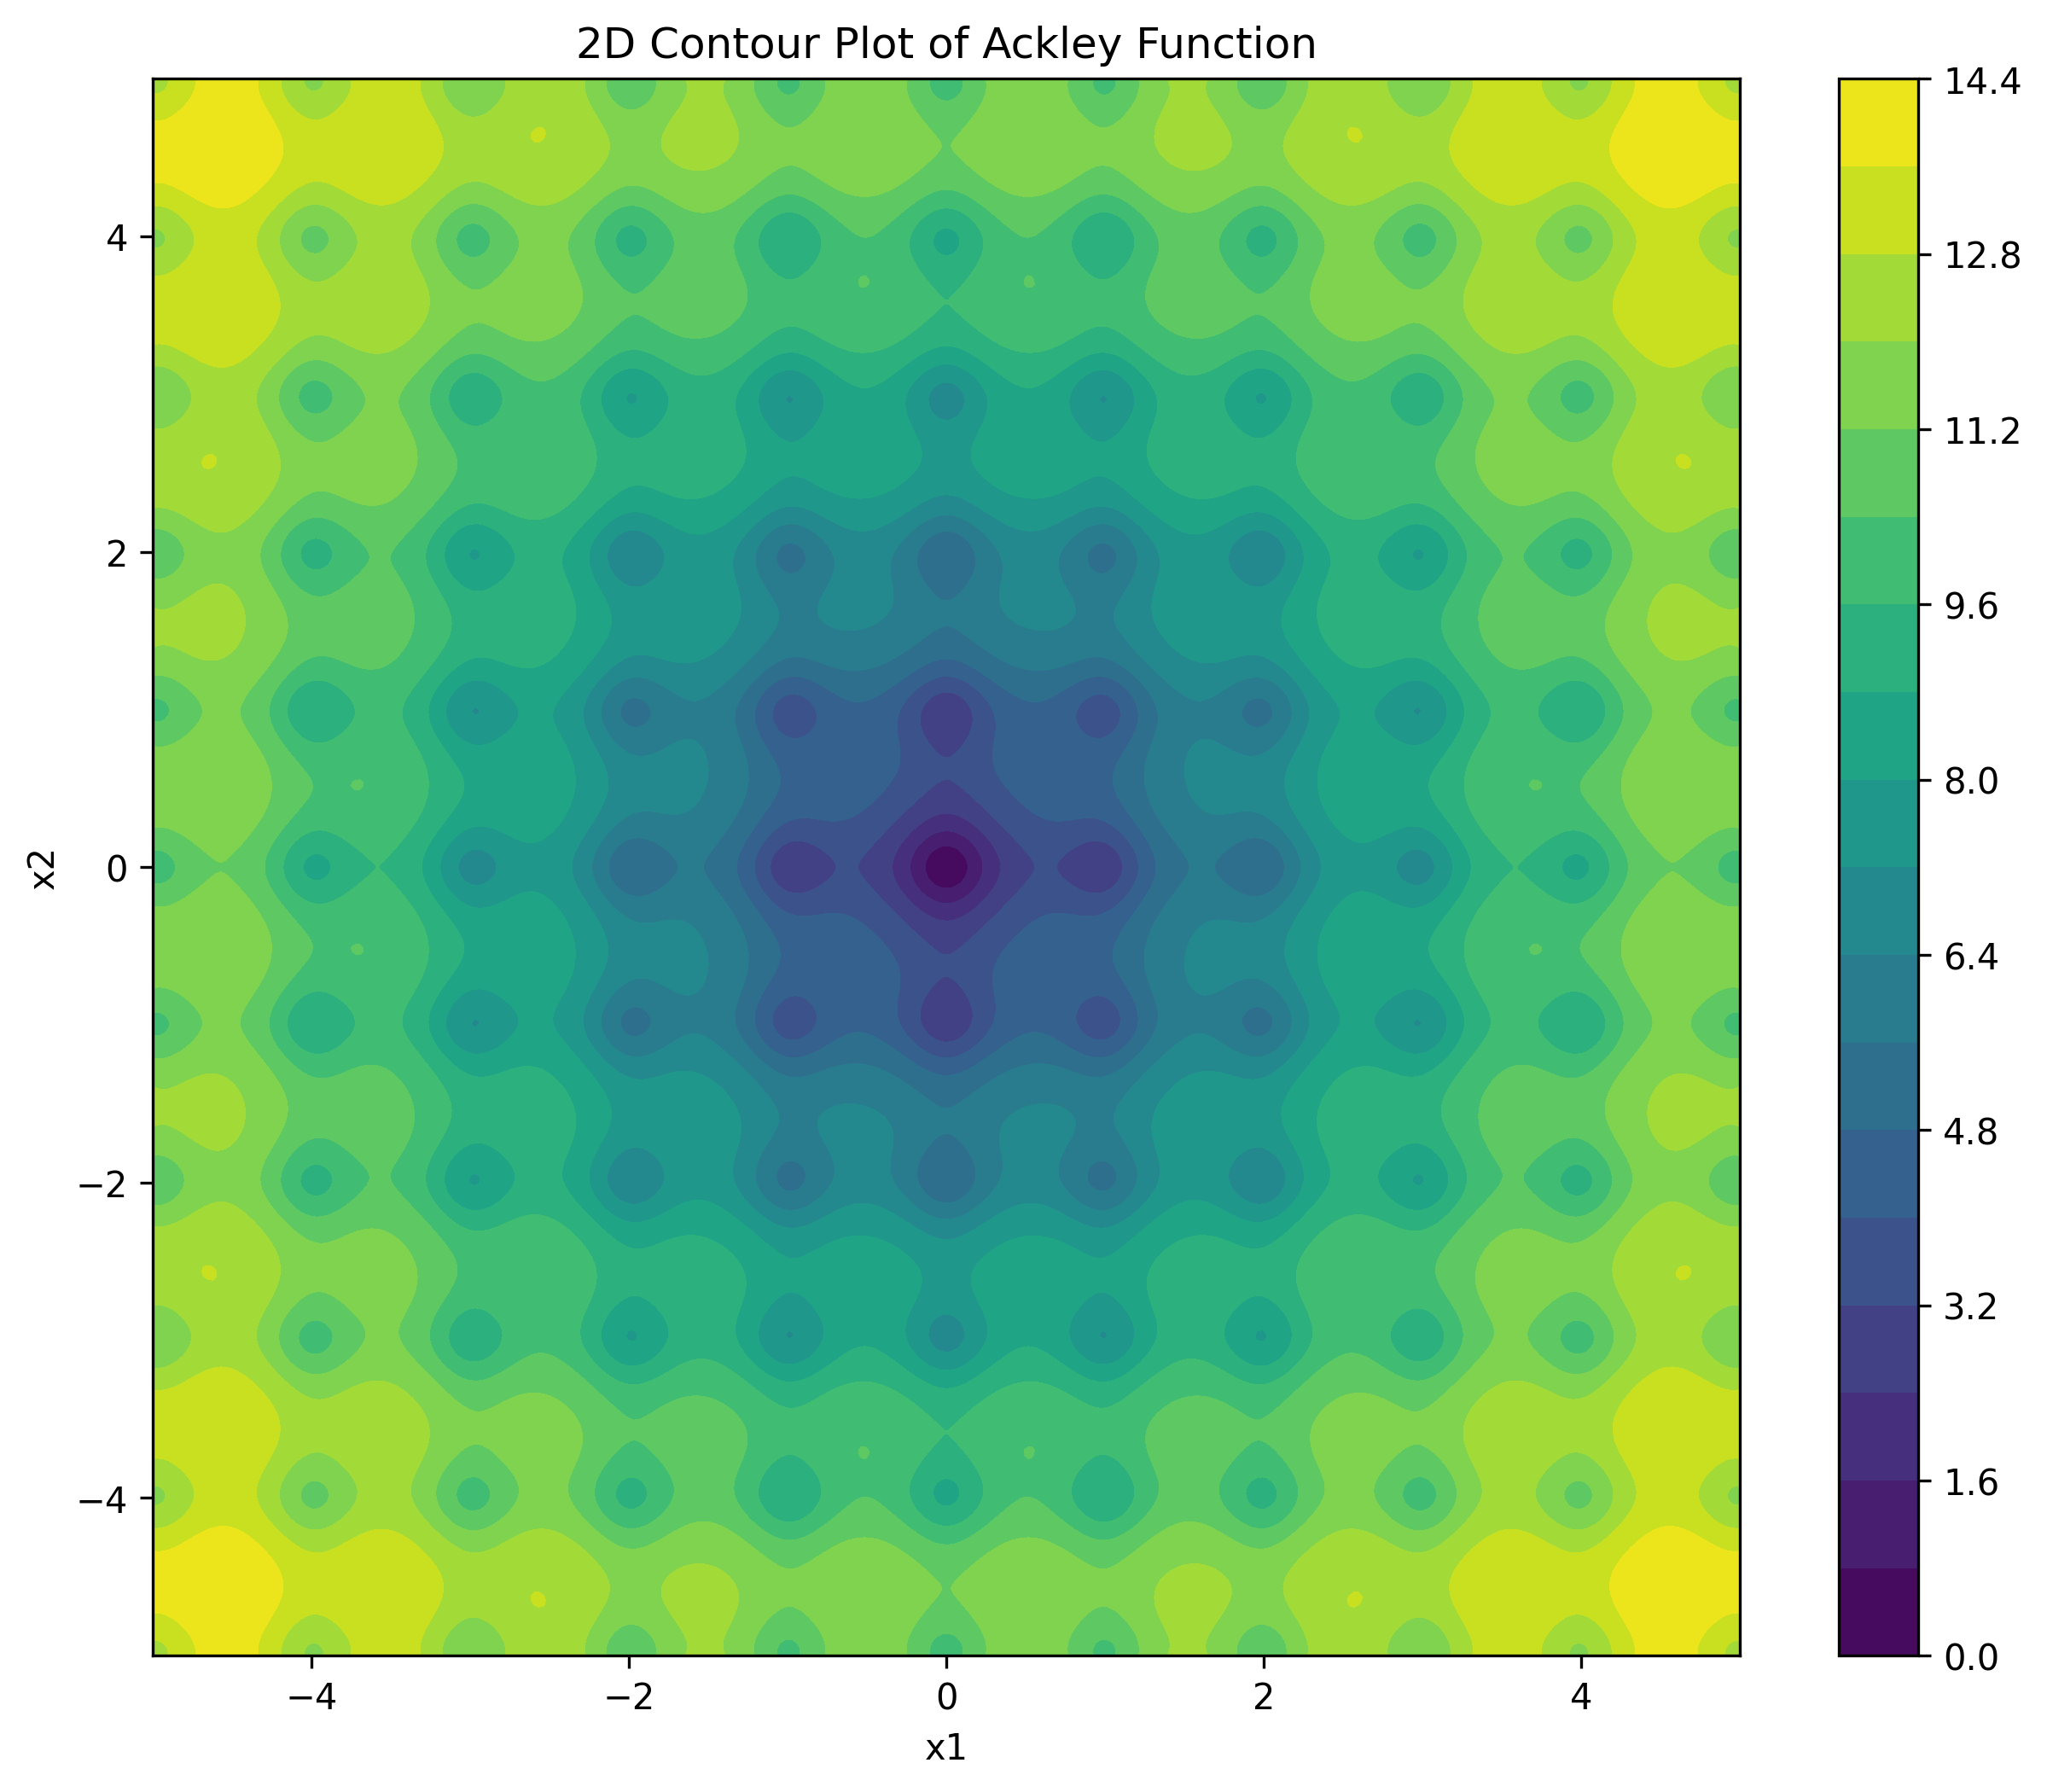
\includegraphics[width=\linewidth]{cec/ackley_2d.png}
		\caption{Dimensi 2}
		\label{fig:ackley-2d}
	\end{subfigure}
	\hfill
	\begin{subfigure}[b]{0.4\textwidth}
		\centering
		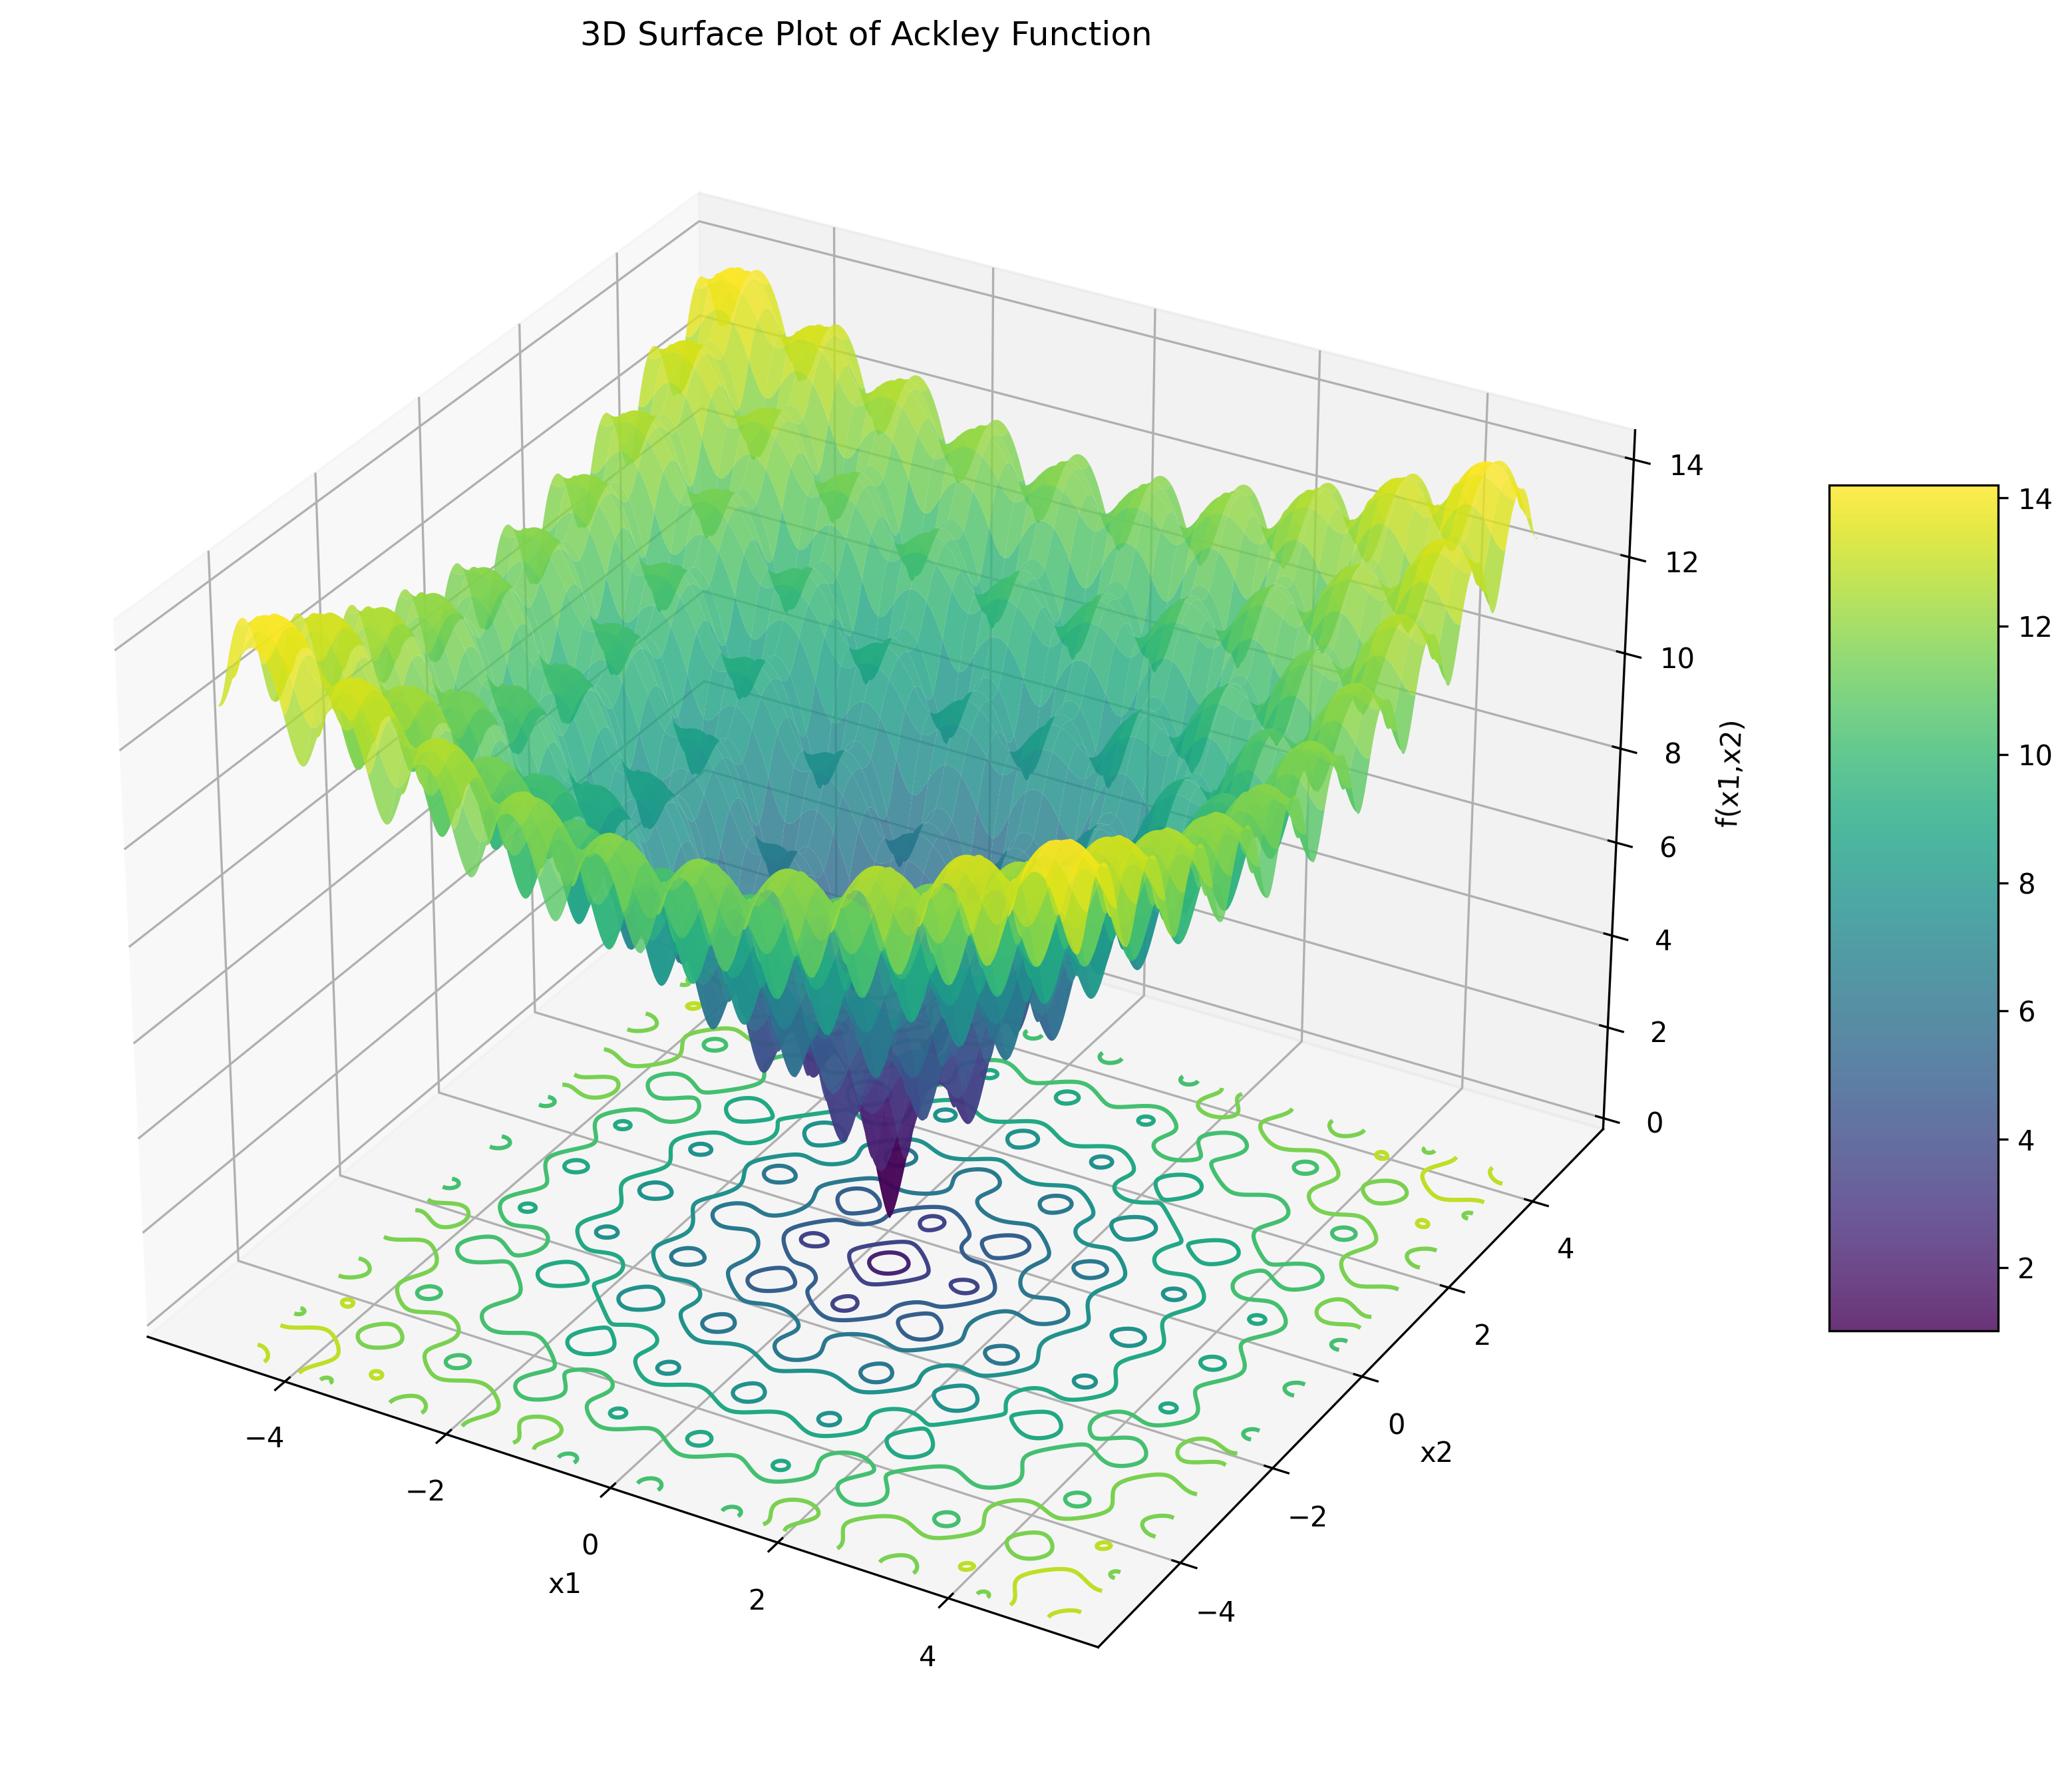
\includegraphics[width=\linewidth]{cec/ackley_3d.png}
		\caption{Dimensi 3}
		\label{fig:ackley-3d}
	\end{subfigure}
	\caption{Tampilan grafik fungsi Ackley pada dimensi dua (\cref{fig:ackley-2d}) dan tiga (\cref{fig:ackley-3d})}
	\label{fig:ackley}
\end{figure}
\begin{equation}
  f_{\text{Ackley}}(\mathrm{x})=-20\exp\left(-0.2\sqrt{\frac{1}{D}\sum_{i=1}^{D}z_i^2} \right)-\exp\left( \frac{1}{D}\sum_{i=1}^{D}\cos\left(2\pi z_i \right) \right) + 20 + e +f_{\text{bias}}
\end{equation}

\subsubsection*{Bent Cigar}
\noindent Properti:
\begin{packed_item}
  \item unimodal
  \item non-separable
  \item convex
\end{packed_item}
\begin{figure}[H]
	\centering
	\begin{subfigure}[b]{0.4\textwidth}
		\centering
		\includegraphics[width=\linewidth]{cec/bent_cigar_2d.png}
		\caption{Dimensi 2}
		\label{fig:bentcigar-2d}
	\end{subfigure}
	\hfill
	\begin{subfigure}[b]{0.4\textwidth}
		\centering
		\includegraphics[width=\linewidth]{cec/bent_cigar_3d.png}
		\caption{Dimensi 3}
		\label{fig:bentcigar-3d}
	\end{subfigure}
	\caption{Tampilan grafik fungsi Bent Cigar pada dimensi dua (\cref{fig:bentcigar-2d}) dan tiga (\cref{fig:bentcigar-3d})}
	\label{fig:bentcigar}
\end{figure}
\begin{equation}
  f_{\text{Bent cigar}}(\mathrm{x})=z_1^2+10^6\sum_{i=2}^{D}z_i^2+f_{\text{bias}}
\end{equation}

\subsubsection*{Different Power}
\noindent Properti:
\begin{packed_item}
  \item unimodal
  \item separable
  \item convex
\end{packed_item}
\begin{figure}[H]
	\centering
	\begin{subfigure}[b]{0.4\textwidth}
		\centering
		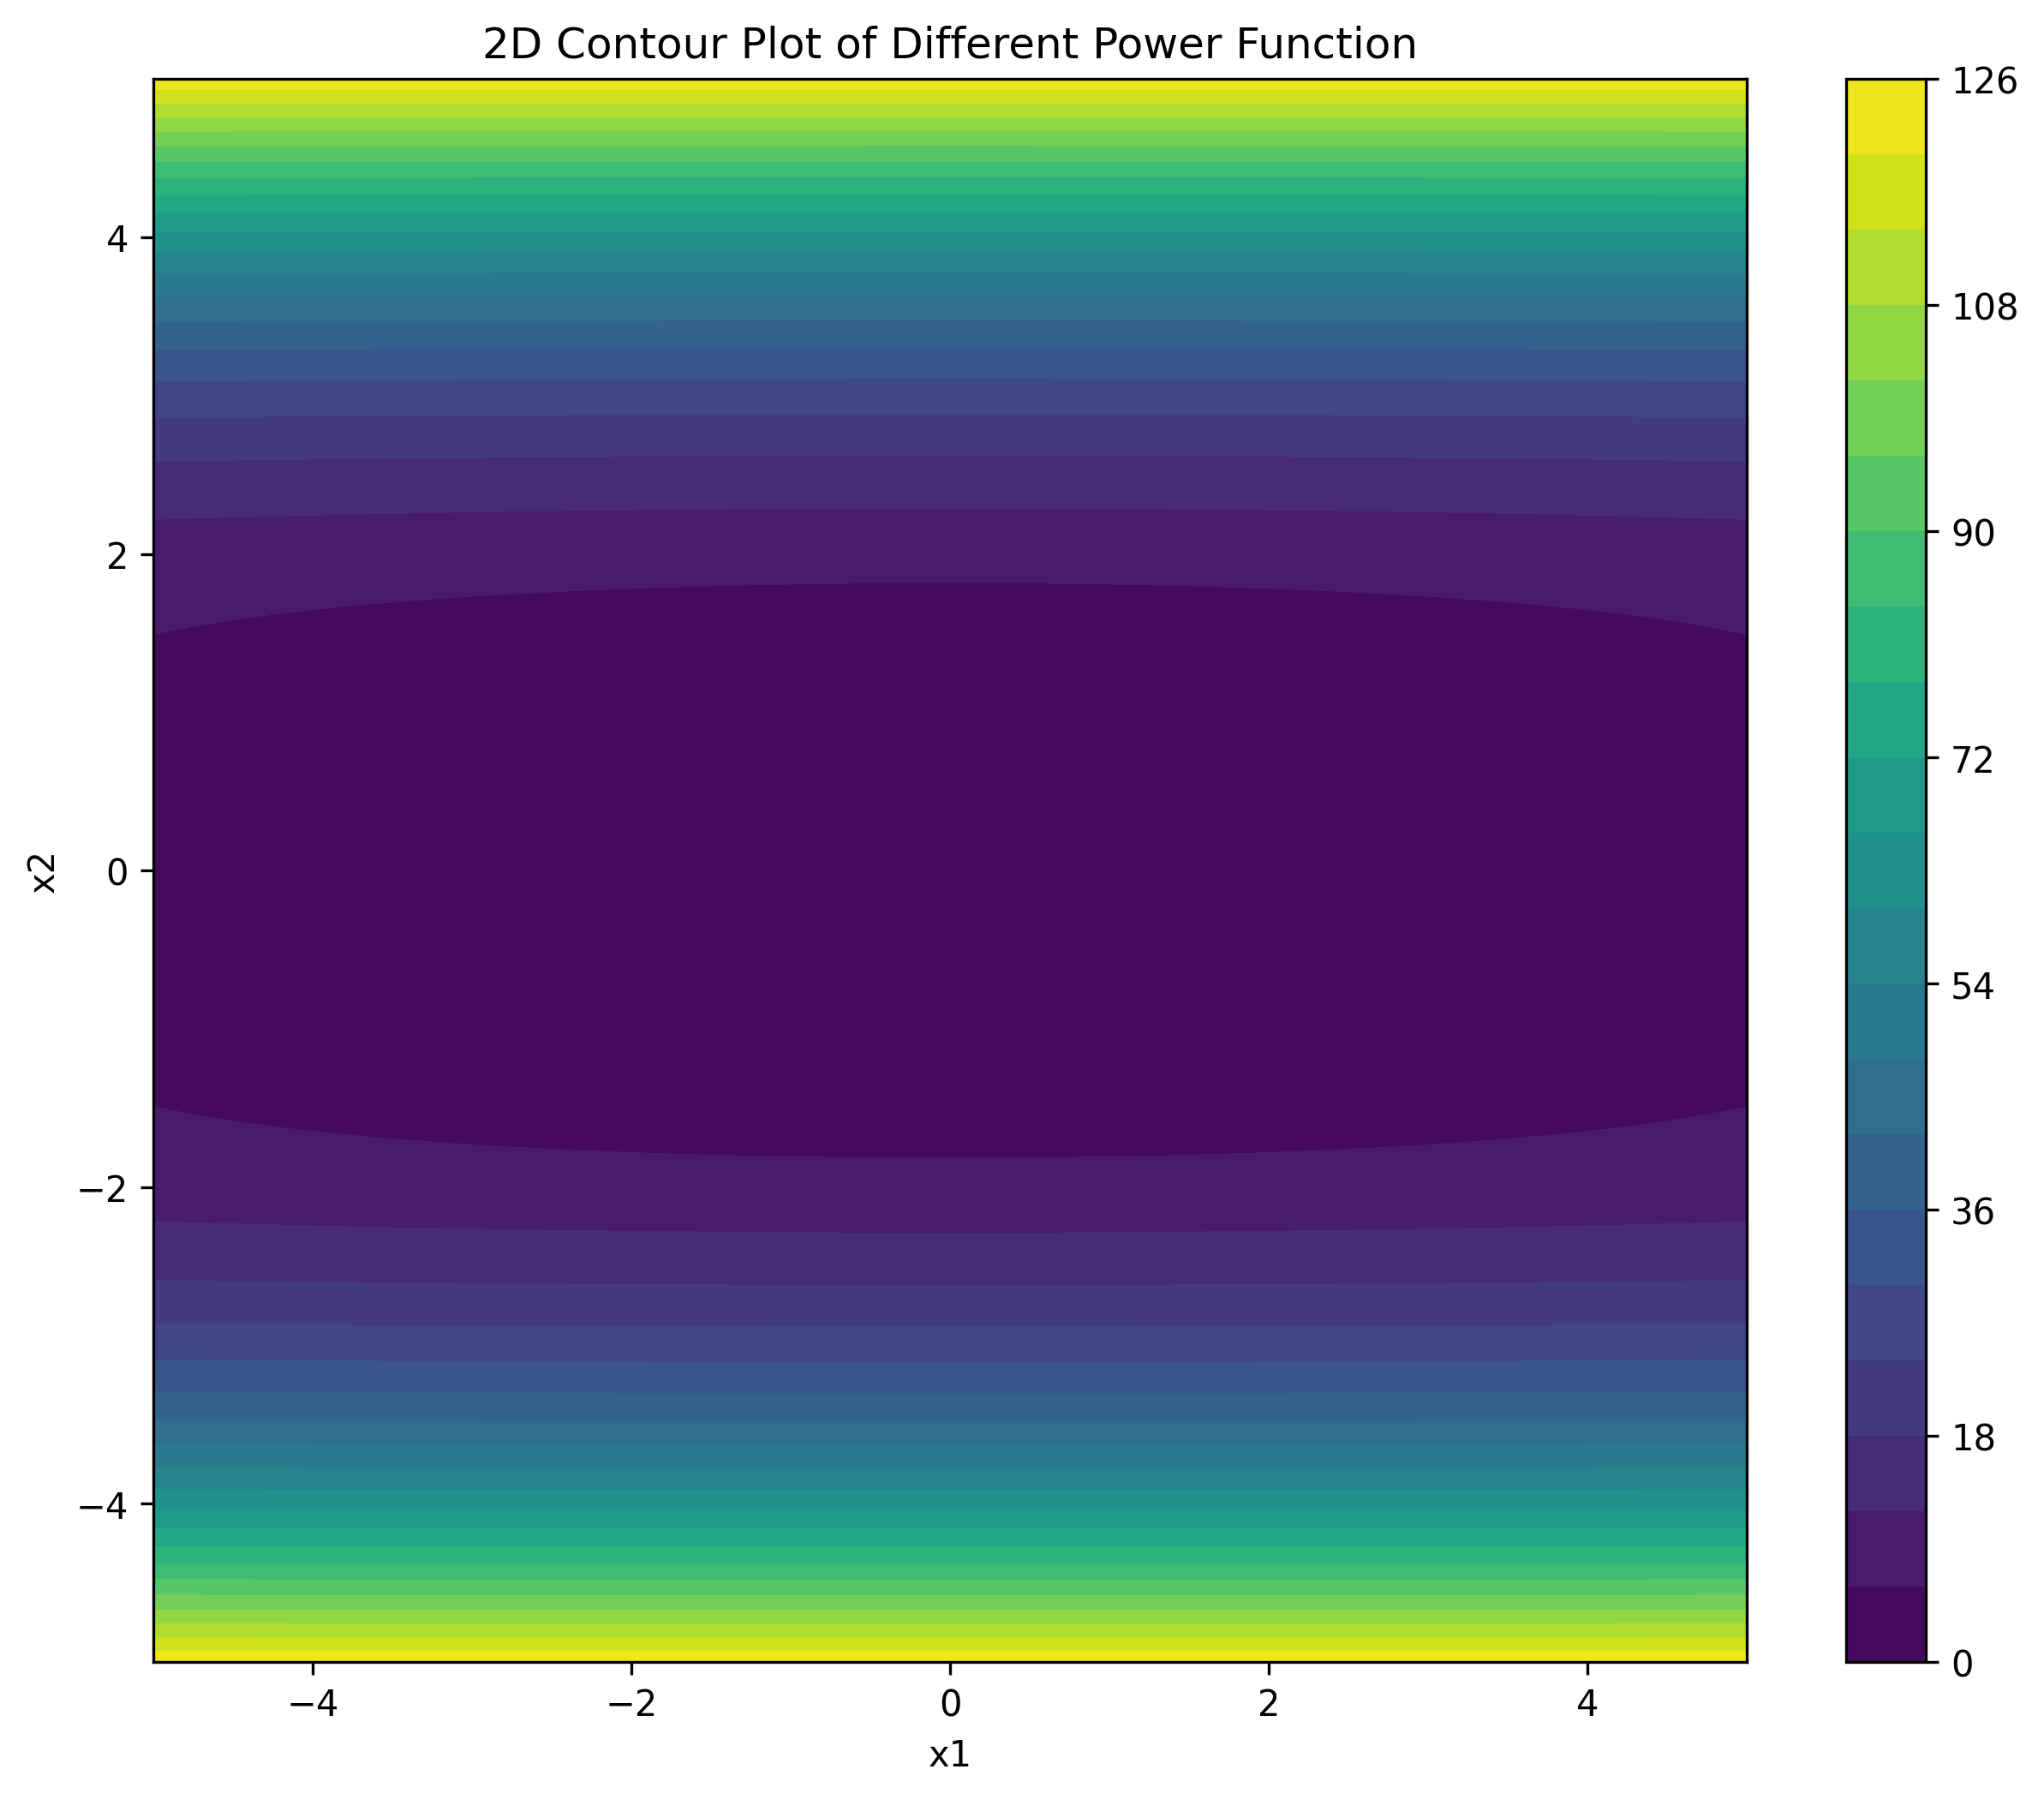
\includegraphics[width=\linewidth]{cec/different_power_2d.png}
		\caption{Dimensi 2}
		\label{fig:diffpower-2d}
	\end{subfigure}
	\hfill
	\begin{subfigure}[b]{0.4\textwidth}
		\centering
		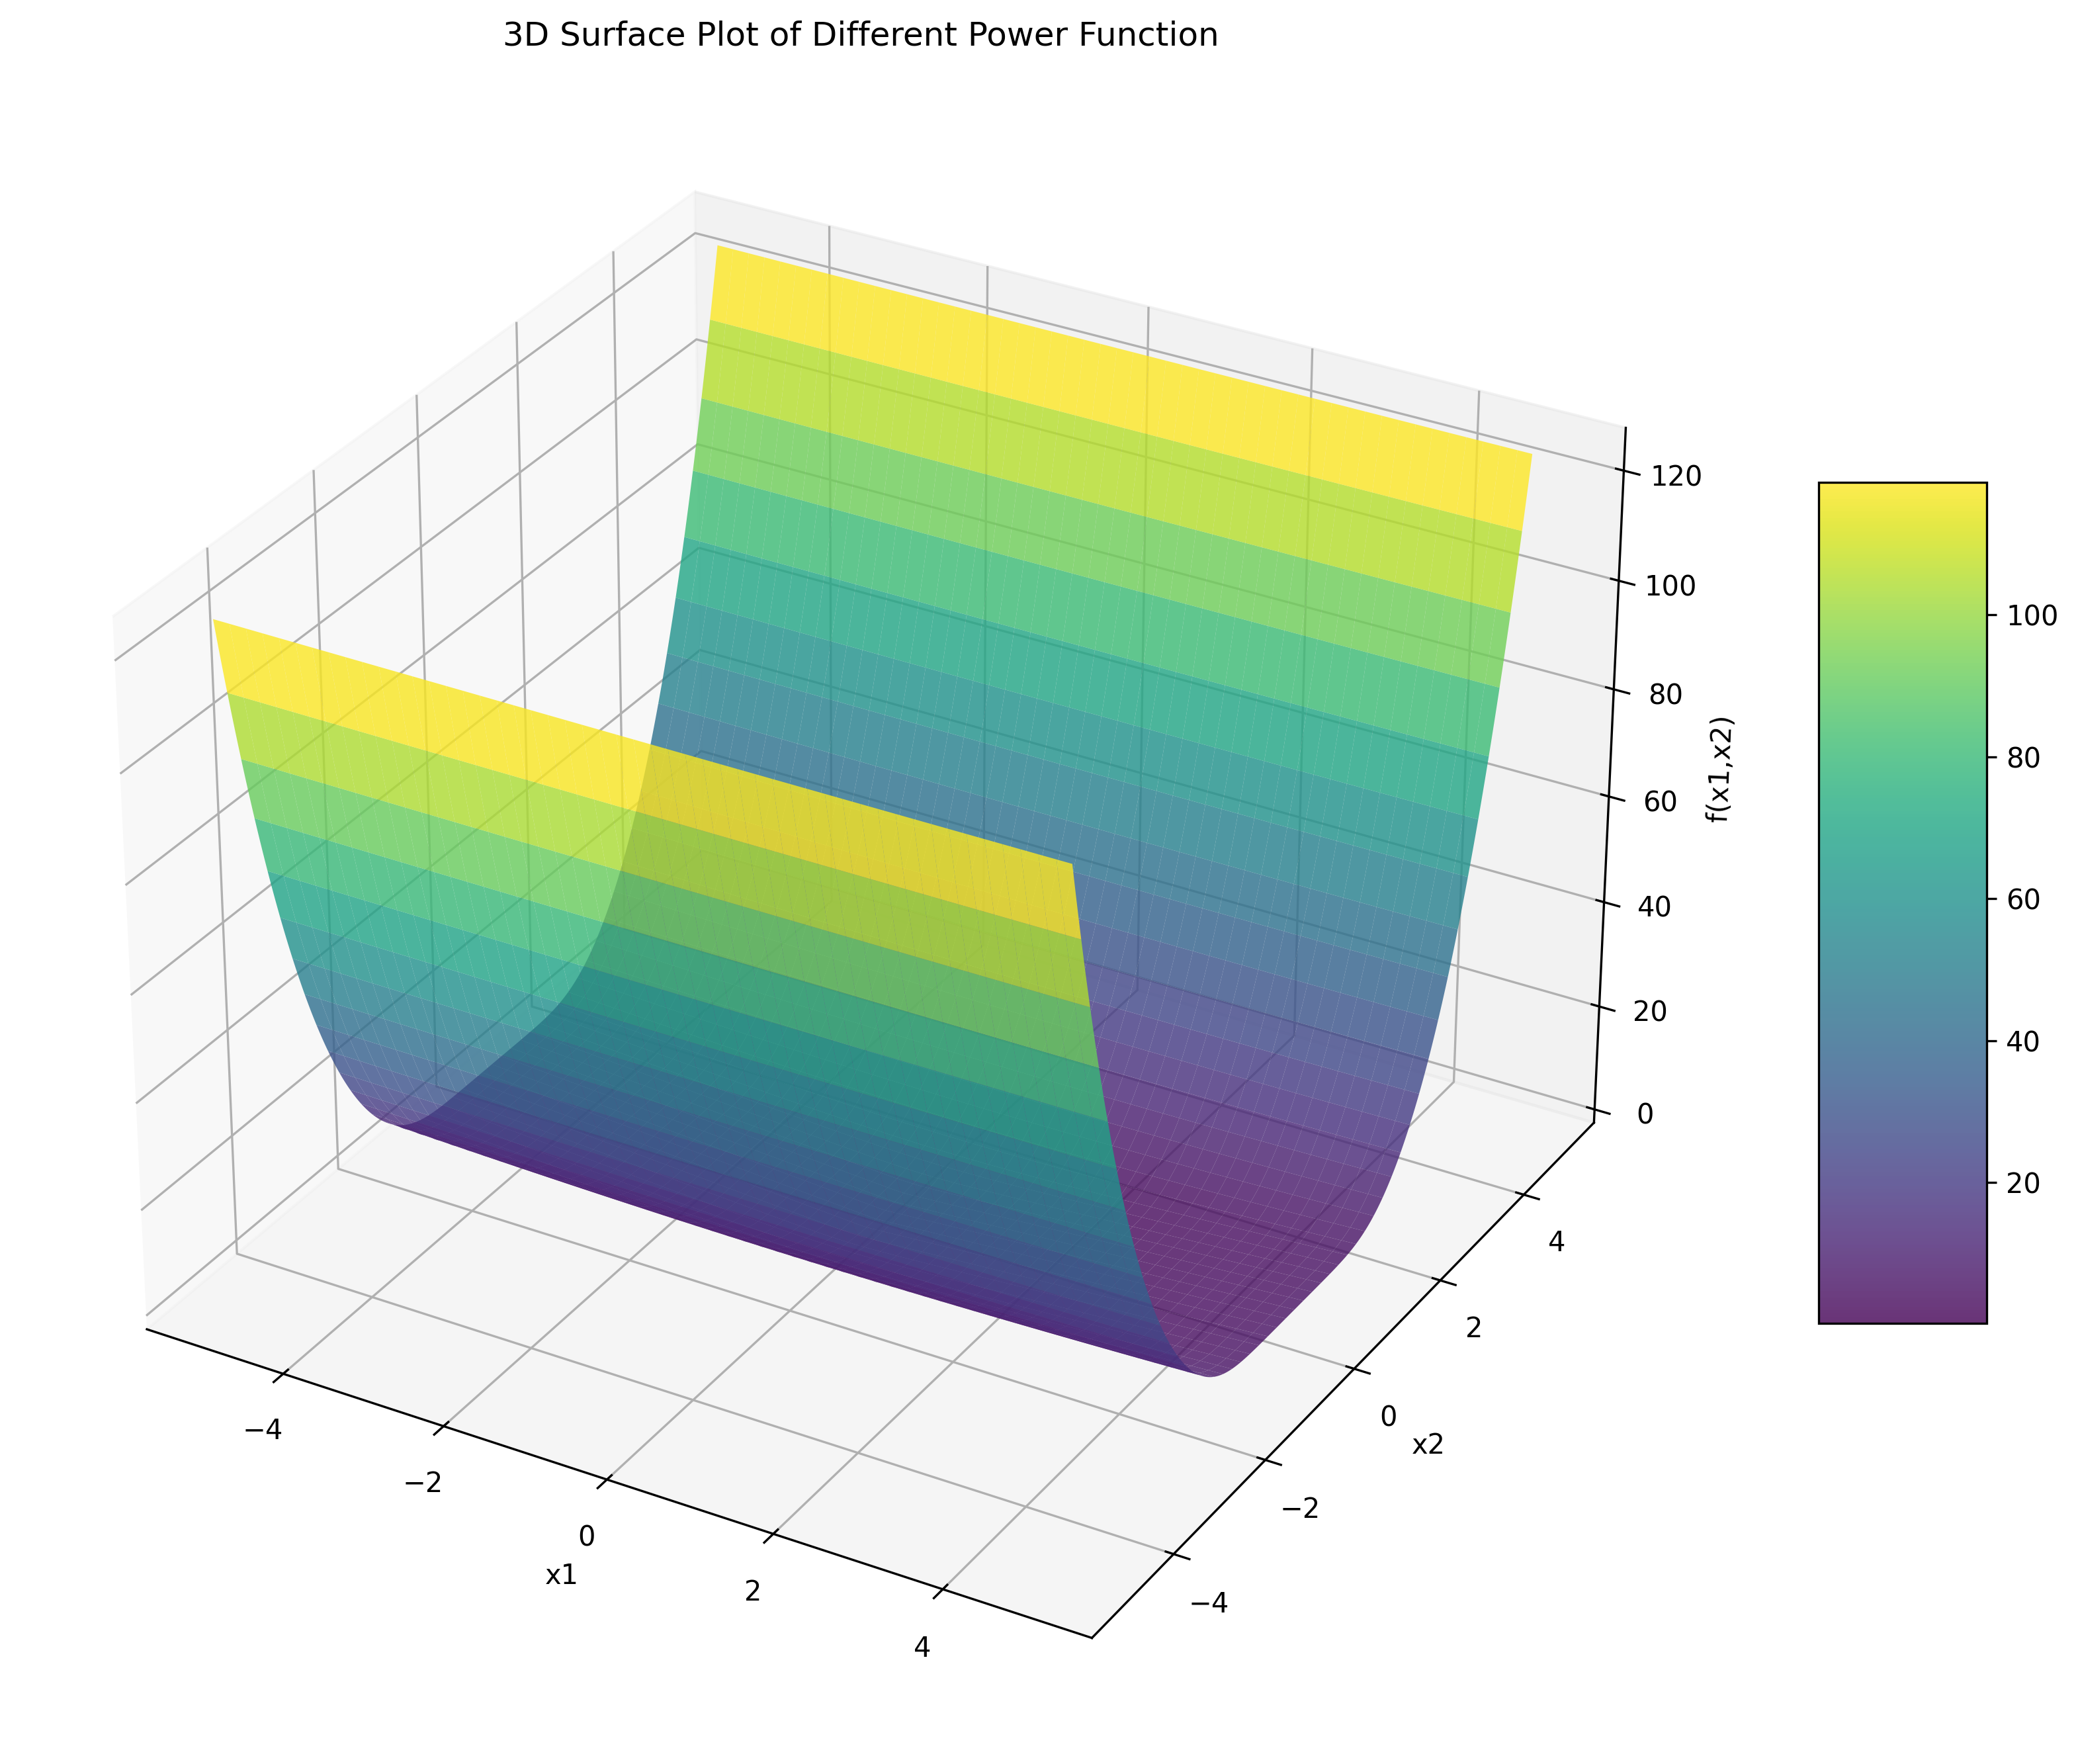
\includegraphics[width=\linewidth]{cec/different_power_3d.png}
		\caption{Dimensi 3}
		\label{fig:diffpower-3d}
	\end{subfigure}
	\caption{Tampilan grafik fungsi Different Power pada dimensi dua (\cref{fig:diffpower-2d}) dan tiga (\cref{fig:diffpower-3d})}
	\label{fig:diffpower}
\end{figure}
\begin{equation}
  f_{\text{Different power}}(\mathrm{x})=\sqrt{\sum_{i=1}^{D}\left| z_i \right|^{2+4\frac{i-1}{D-1}} }+f_{\text{bias}}
\end{equation}

\subsubsection*{Discus}
\noindent Properti:
\begin{packed_item}
  \item unimodal
  \item non-separable
  \item convex
\end{packed_item}
\begin{figure}[H]
	\centering
	\begin{subfigure}[b]{0.4\textwidth}
		\centering
		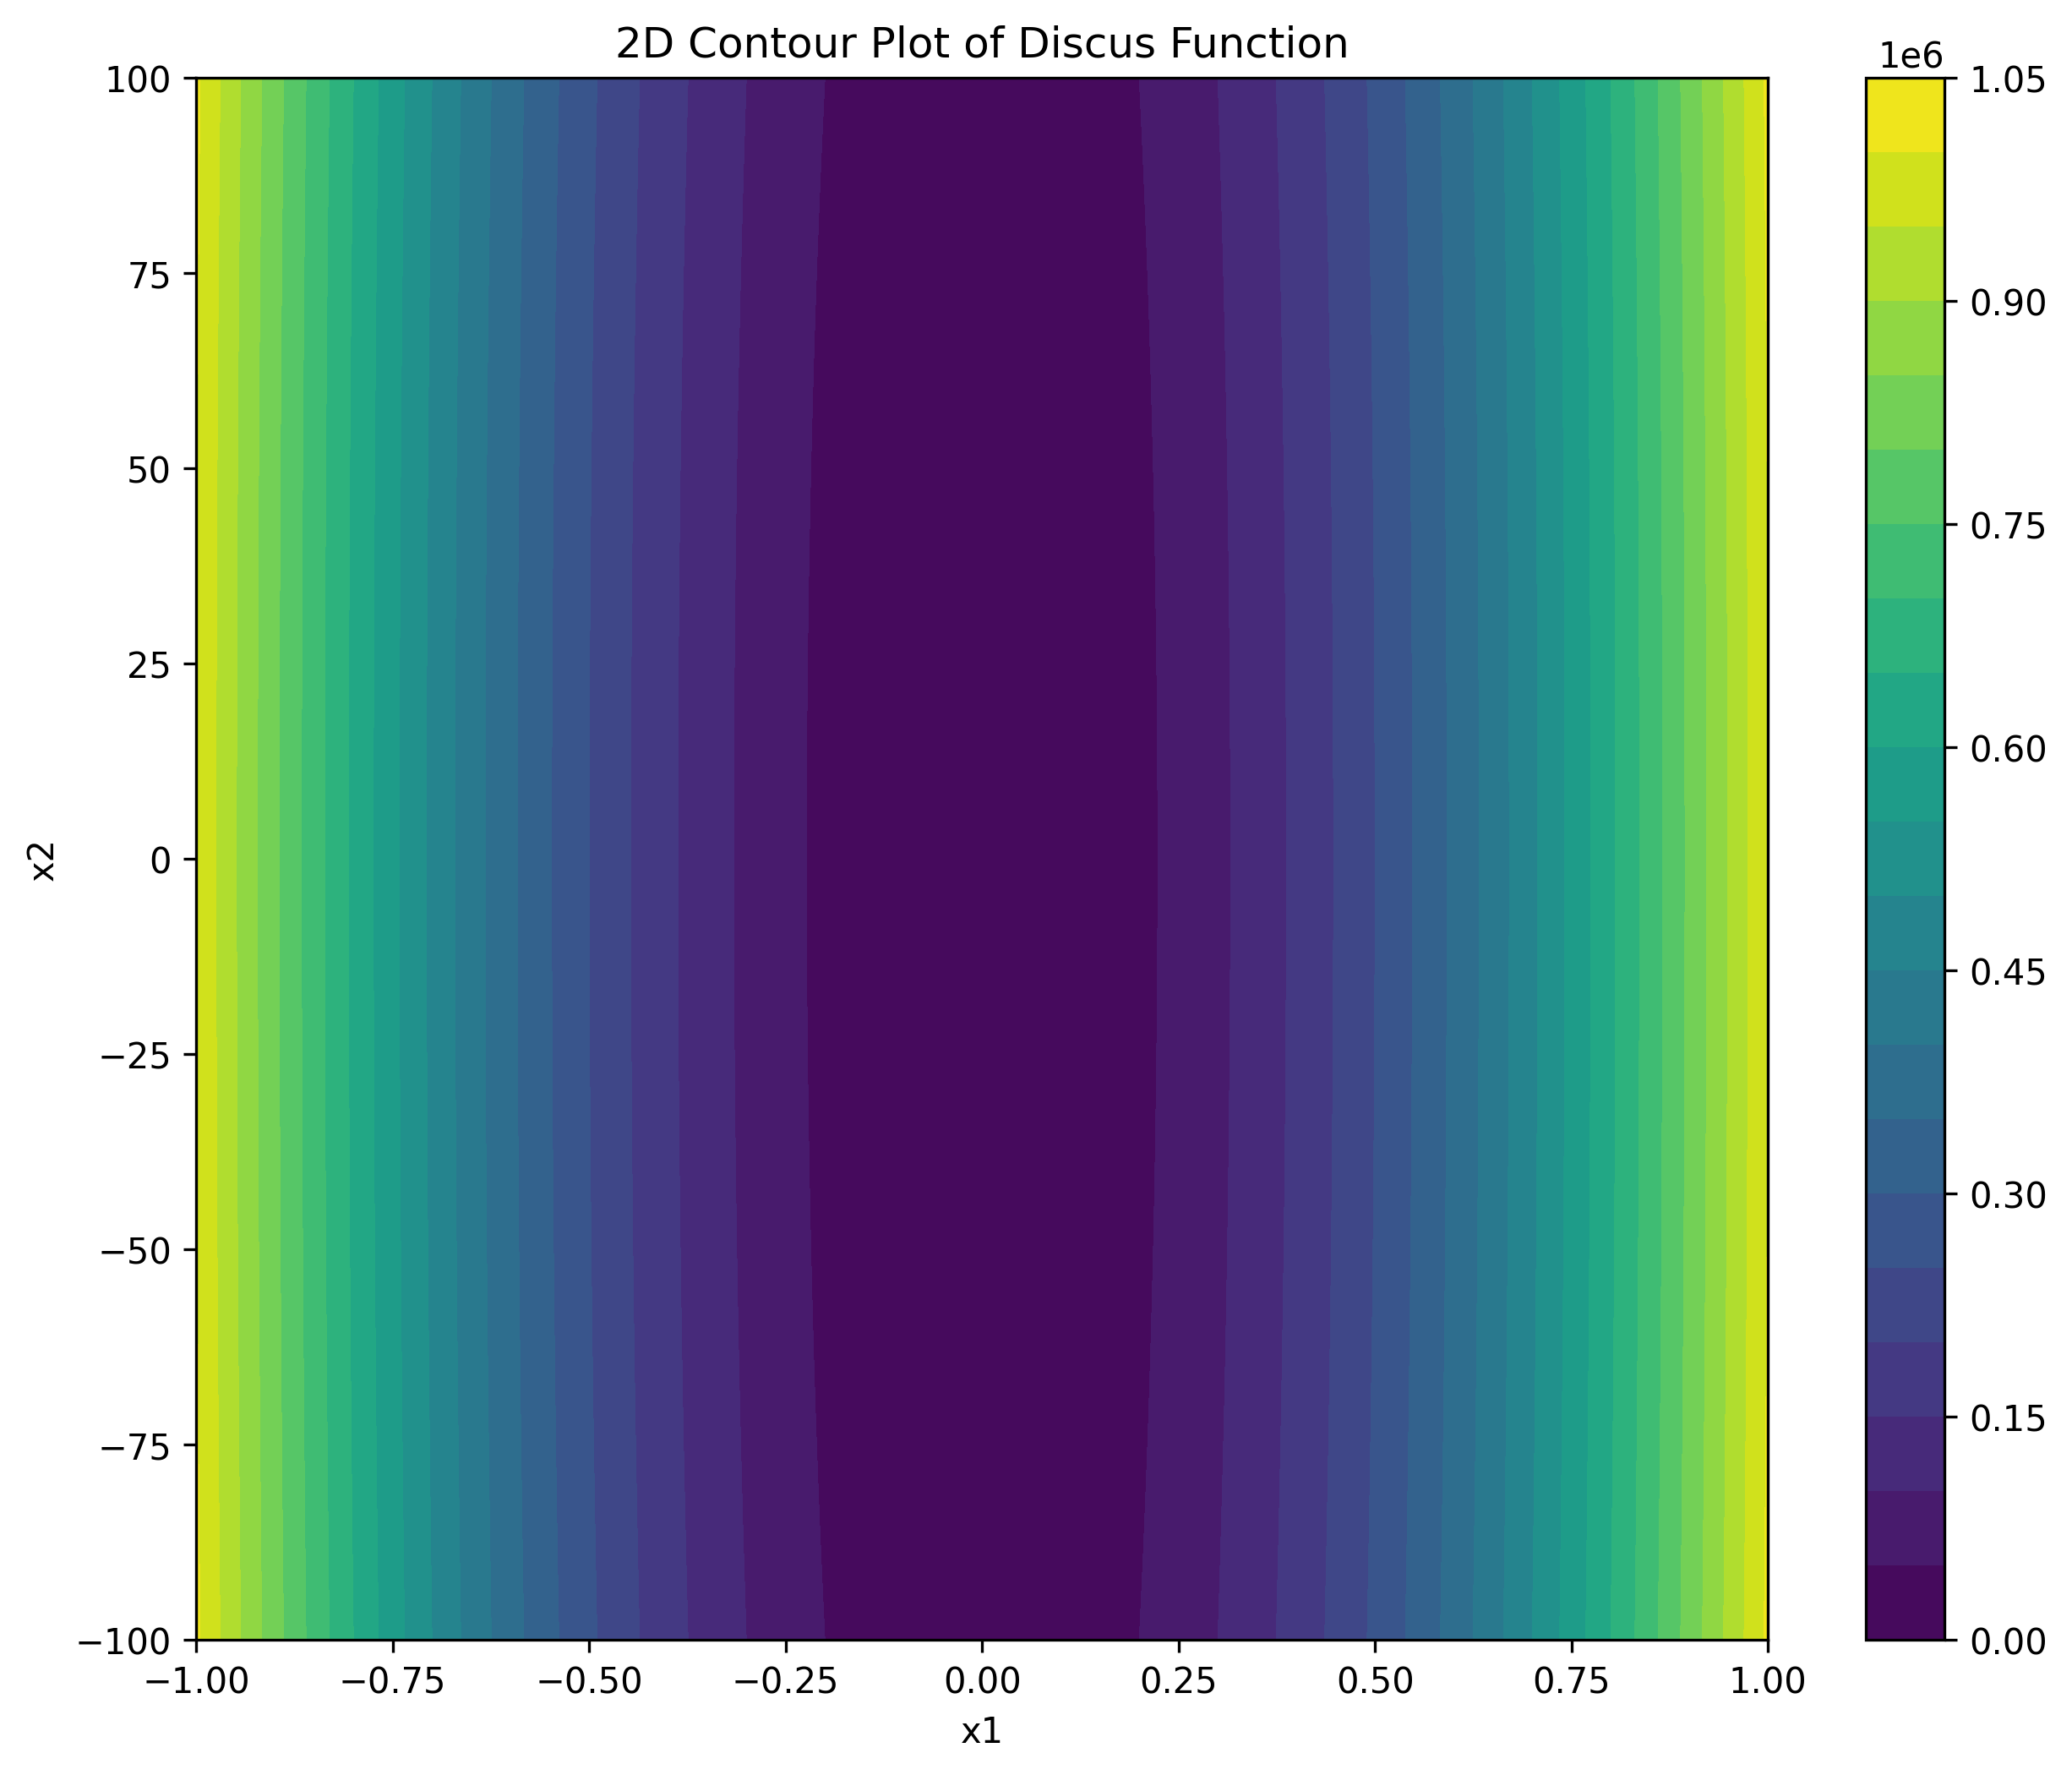
\includegraphics[width=\linewidth]{cec/discus_2d.png}
		\caption{Dimensi 2}
		\label{fig:discus-2d}
	\end{subfigure}
	\hfill
	\begin{subfigure}[b]{0.4\textwidth}
		\centering
		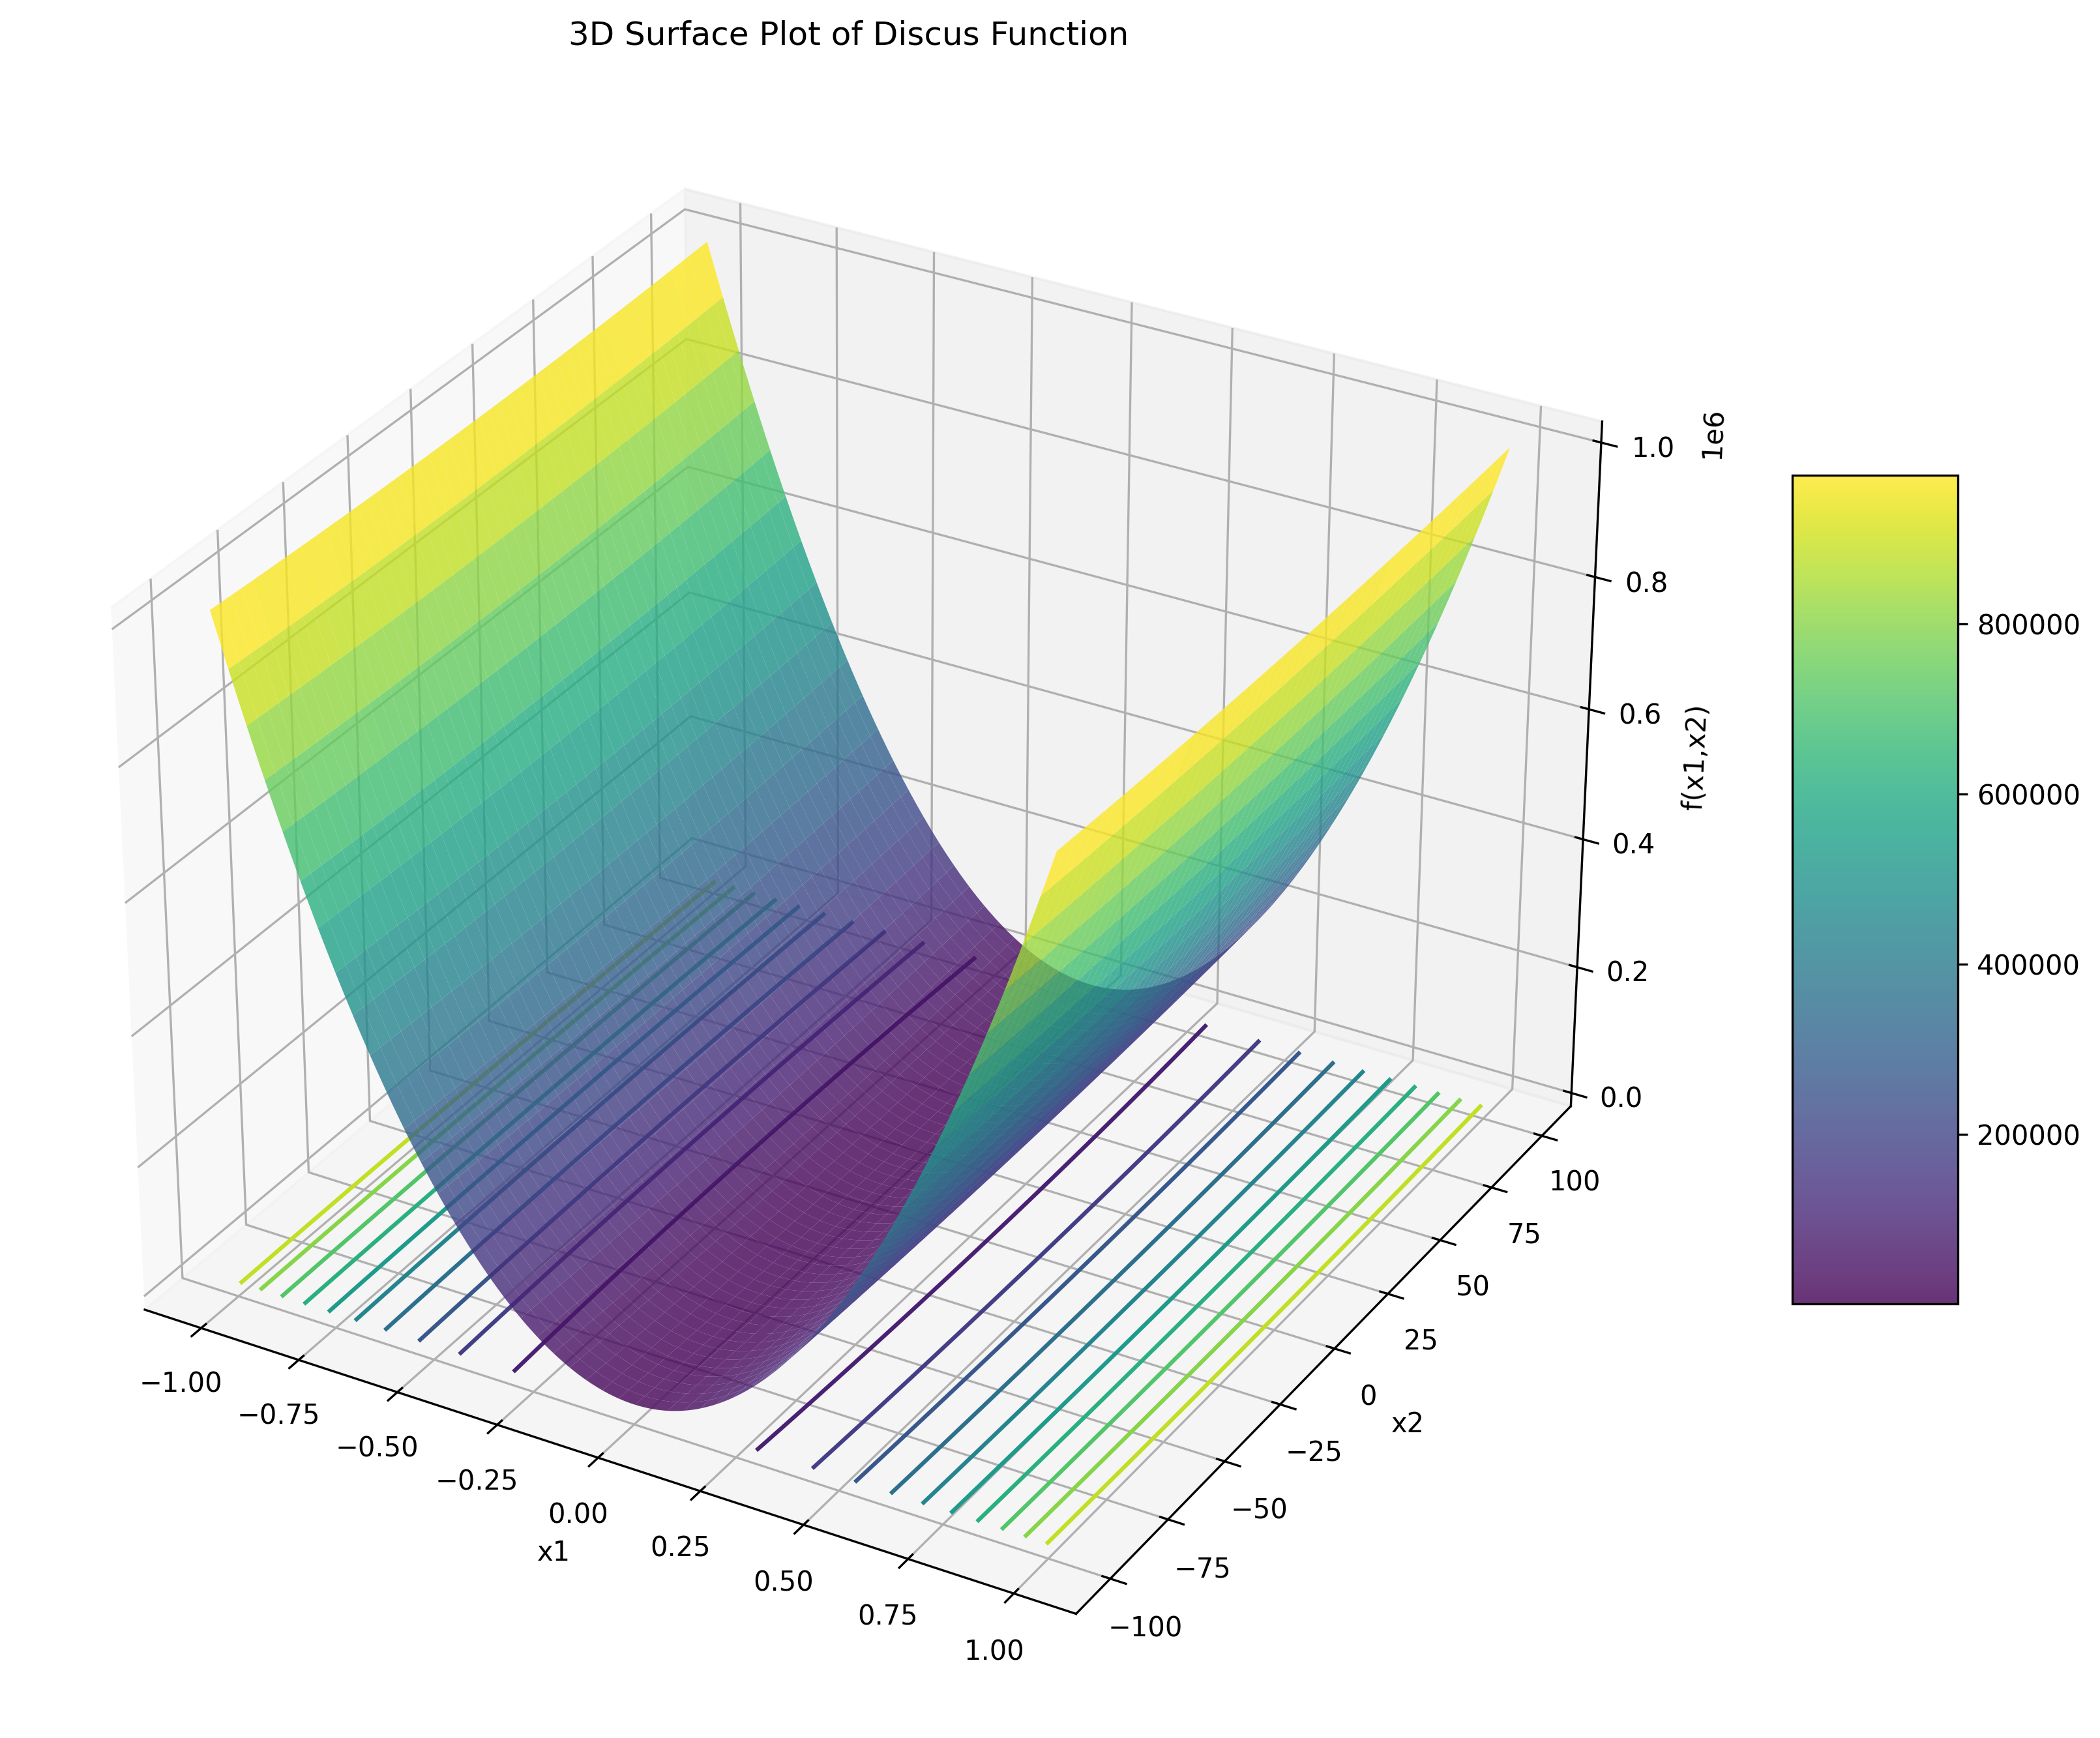
\includegraphics[width=\linewidth]{cec/discus_3d.png}
		\caption{Dimensi 3}
		\label{fig:discus-3d}
	\end{subfigure}
	\caption{Tampilan grafik fungsi Discus pada dimensi dua (\cref{fig:discus-2d}) dan tiga (\cref{fig:discus-3d})}
	\label{fig:discus}
\end{figure}
\begin{equation}
  f_{\text{Discus}}(\mathrm{x})=10^6z_1^2+\sum_{i=2}^{D}z_i^2+f_{\text{bias}}
\end{equation}

\subsubsection*{Ellipsoid}
\noindent Properti:
\begin{packed_item}
  \item unimodal
  \item convex
\end{packed_item}
\begin{figure}[H]
	\centering
	\begin{subfigure}[b]{0.4\textwidth}
		\centering
		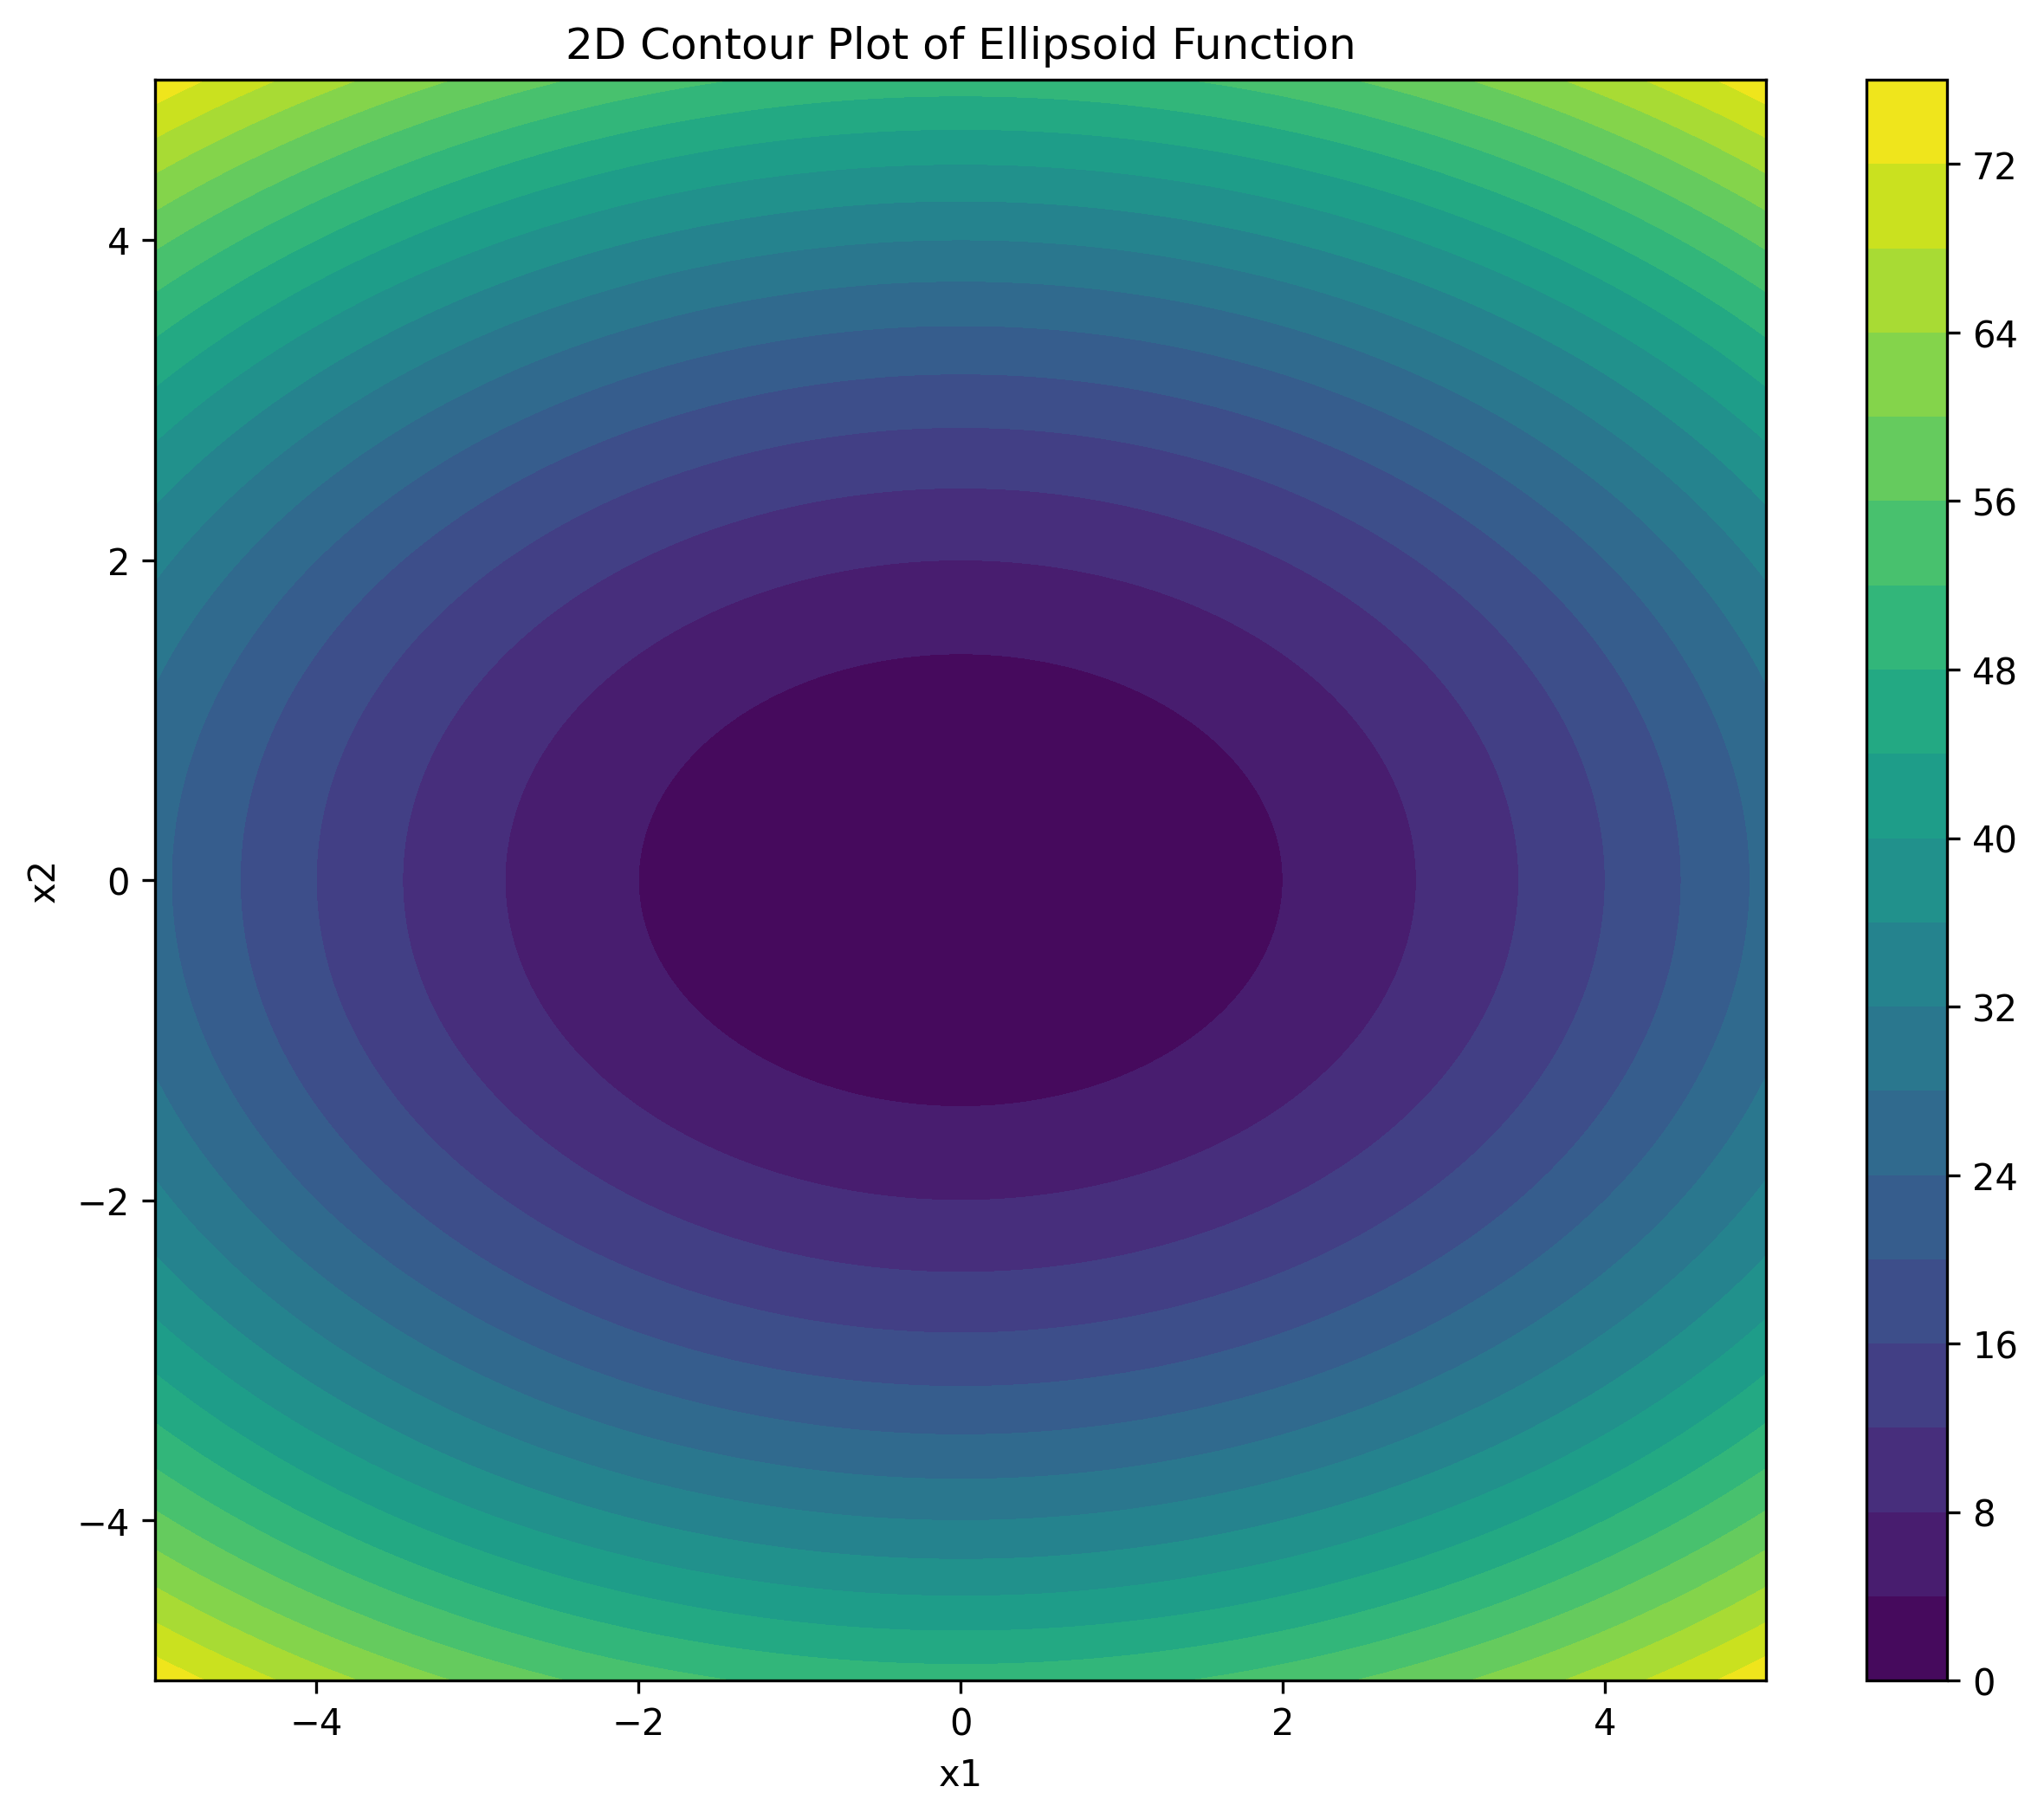
\includegraphics[width=\linewidth]{cec/ellipsoid_2d.png}
		\caption{Dimensi 2}
		\label{fig:ellipsoid-2d}
	\end{subfigure}
	\hfill
	\begin{subfigure}[b]{0.4\textwidth}
		\centering
		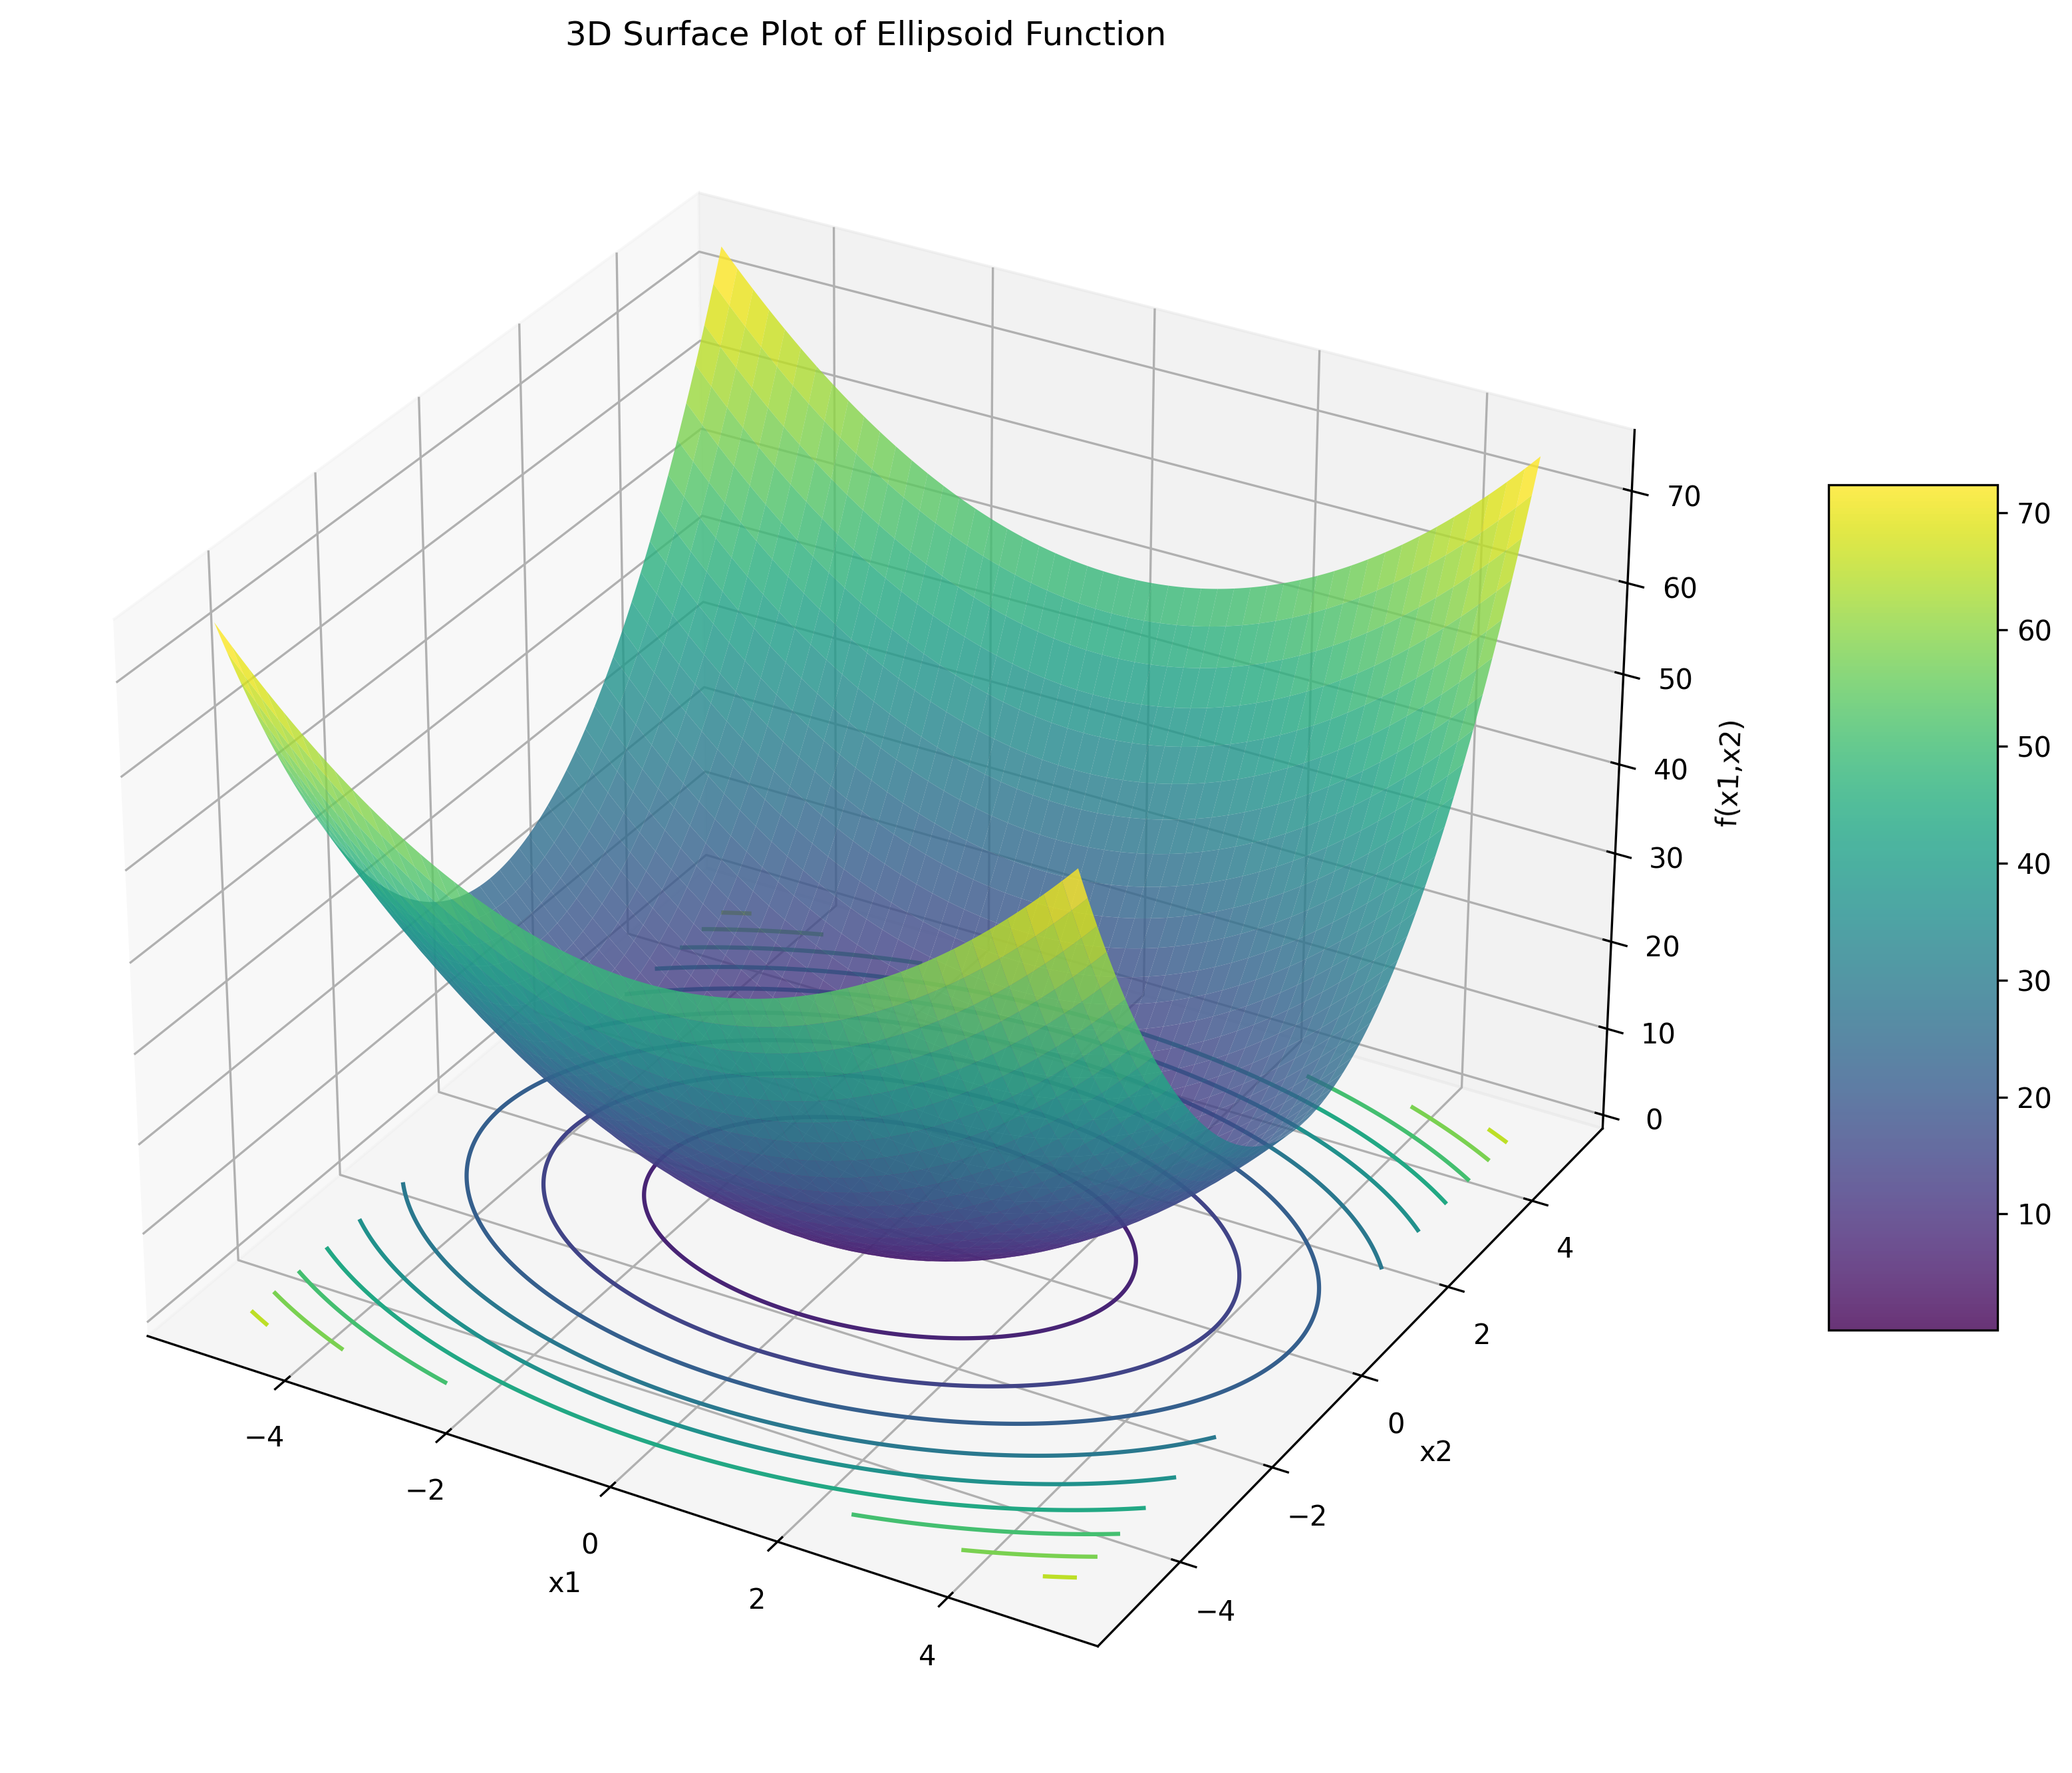
\includegraphics[width=\linewidth]{cec/ellipsoid_3d.png}
		\caption{Dimensi 3}
		\label{fig:ellipsoid-3d}
	\end{subfigure}
	\caption{Tampilan grafik fungsi Ellipsoid pada dimensi dua (\cref{fig:ellipsoid-2d}) dan tiga (\cref{fig:ellipsoid-3d})}
	\label{fig:ellipsoid}
\end{figure}
\begin{equation}
  f_{\text{Ellipsoid}}(\mathrm{x})=\sum_{i=1}^{D}iz_i^2  +f_{\text{bias}}
\end{equation}

\subsubsection*{Elliptic}
\noindent Properti:
\begin{packed_item}
  \item unimodal
  \item convex
  \item non-separable
  \item quadric ill-conditioned
  \item smooth local irregularities
\end{packed_item}
\begin{figure}[H]
	\centering
	\begin{subfigure}[b]{0.4\textwidth}
		\centering
		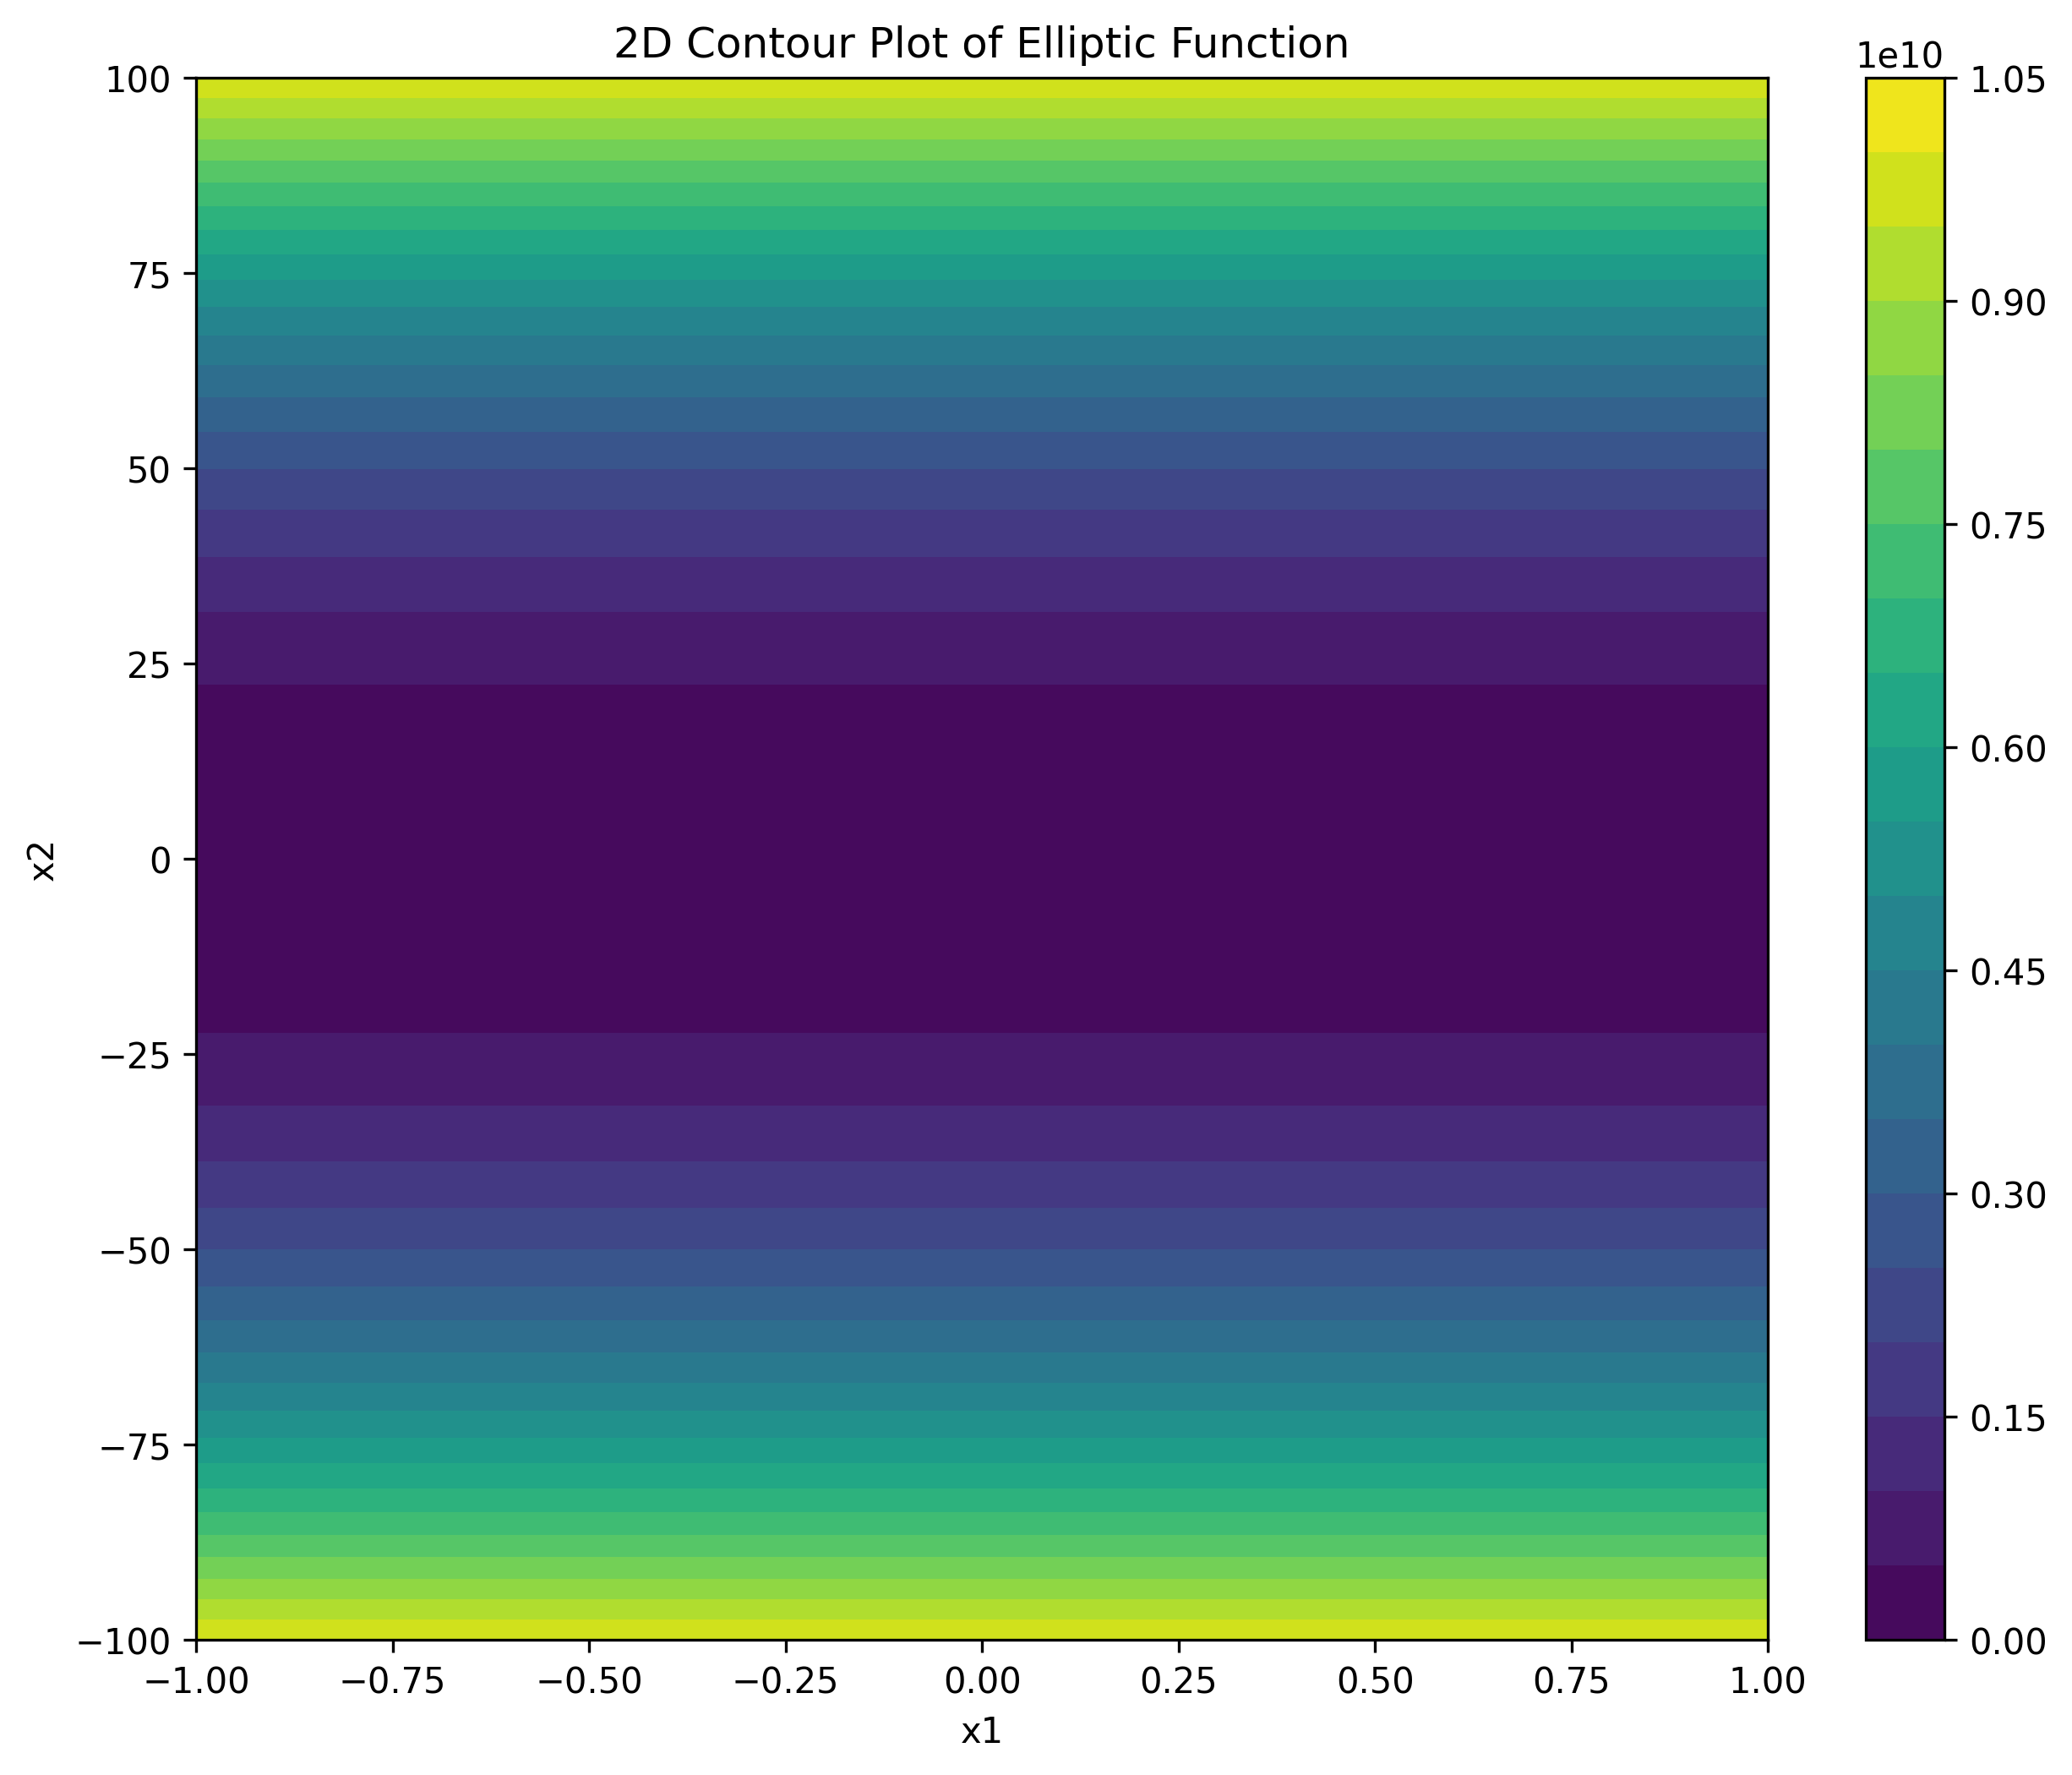
\includegraphics[width=\linewidth]{cec/elliptic_2d.png}
		\caption{Dimensi 2}
		\label{fig:elliptic-2d}
	\end{subfigure}
	\hfill
	\begin{subfigure}[b]{0.4\textwidth}
		\centering
		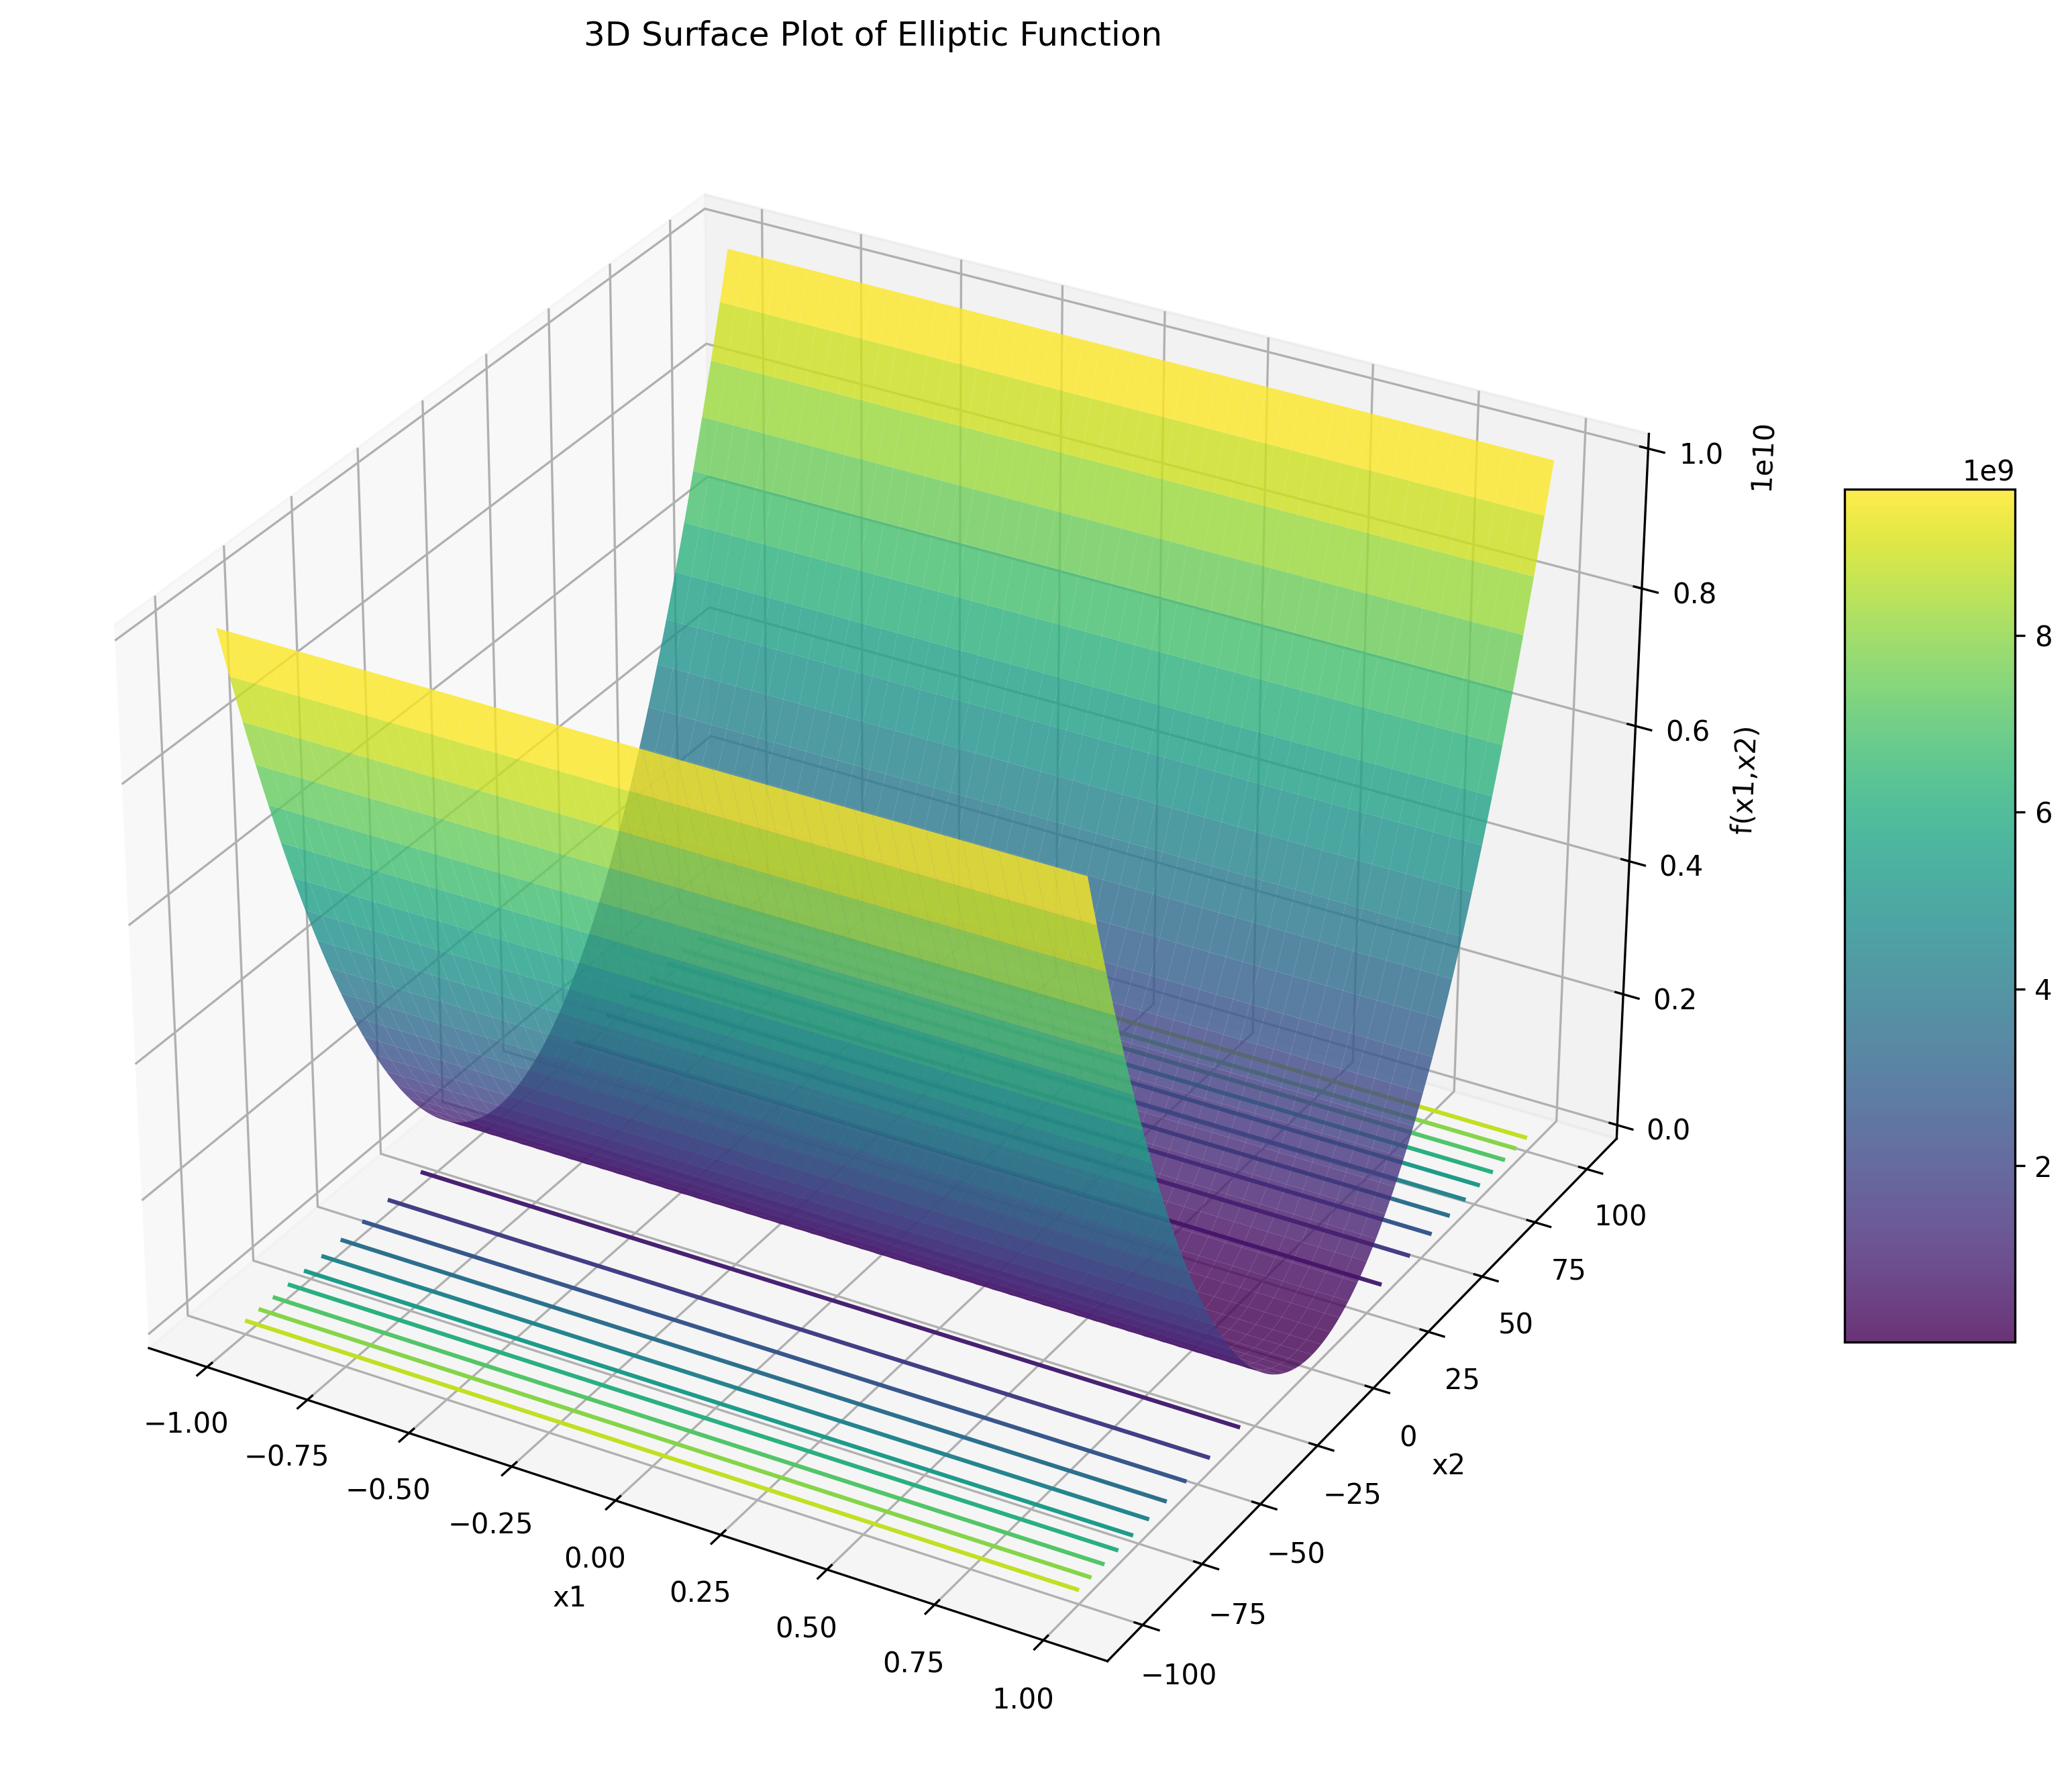
\includegraphics[width=\linewidth]{cec/elliptic_3d.png}
		\caption{Dimensi 3}
		\label{fig:elliptic-3d}
	\end{subfigure}
	\caption{Tampilan grafik fungsi Elliptic pada dimensi dua (\cref{fig:elliptic-2d}) dan tiga (\cref{fig:elliptic-3d})}
	\label{fig:elliptic}
\end{figure}
\begin{equation}
  f_{\text{Elliptic}}(\mathrm{x})= \sum_{i=1}^{D} \left( 10^6\right)^{\frac{i-1}{D-1}} z_i^2 +f_{\text{bias}}
\end{equation}

\subsubsection*{Expanded schaffer f6}
\noindent Properti:
\begin{packed_item}
  \item multimodal
  \item non-convex
  \item non-separable
\end{packed_item}
\begin{figure}[H]
	\centering
	\begin{subfigure}[b]{0.4\textwidth}
		\centering
		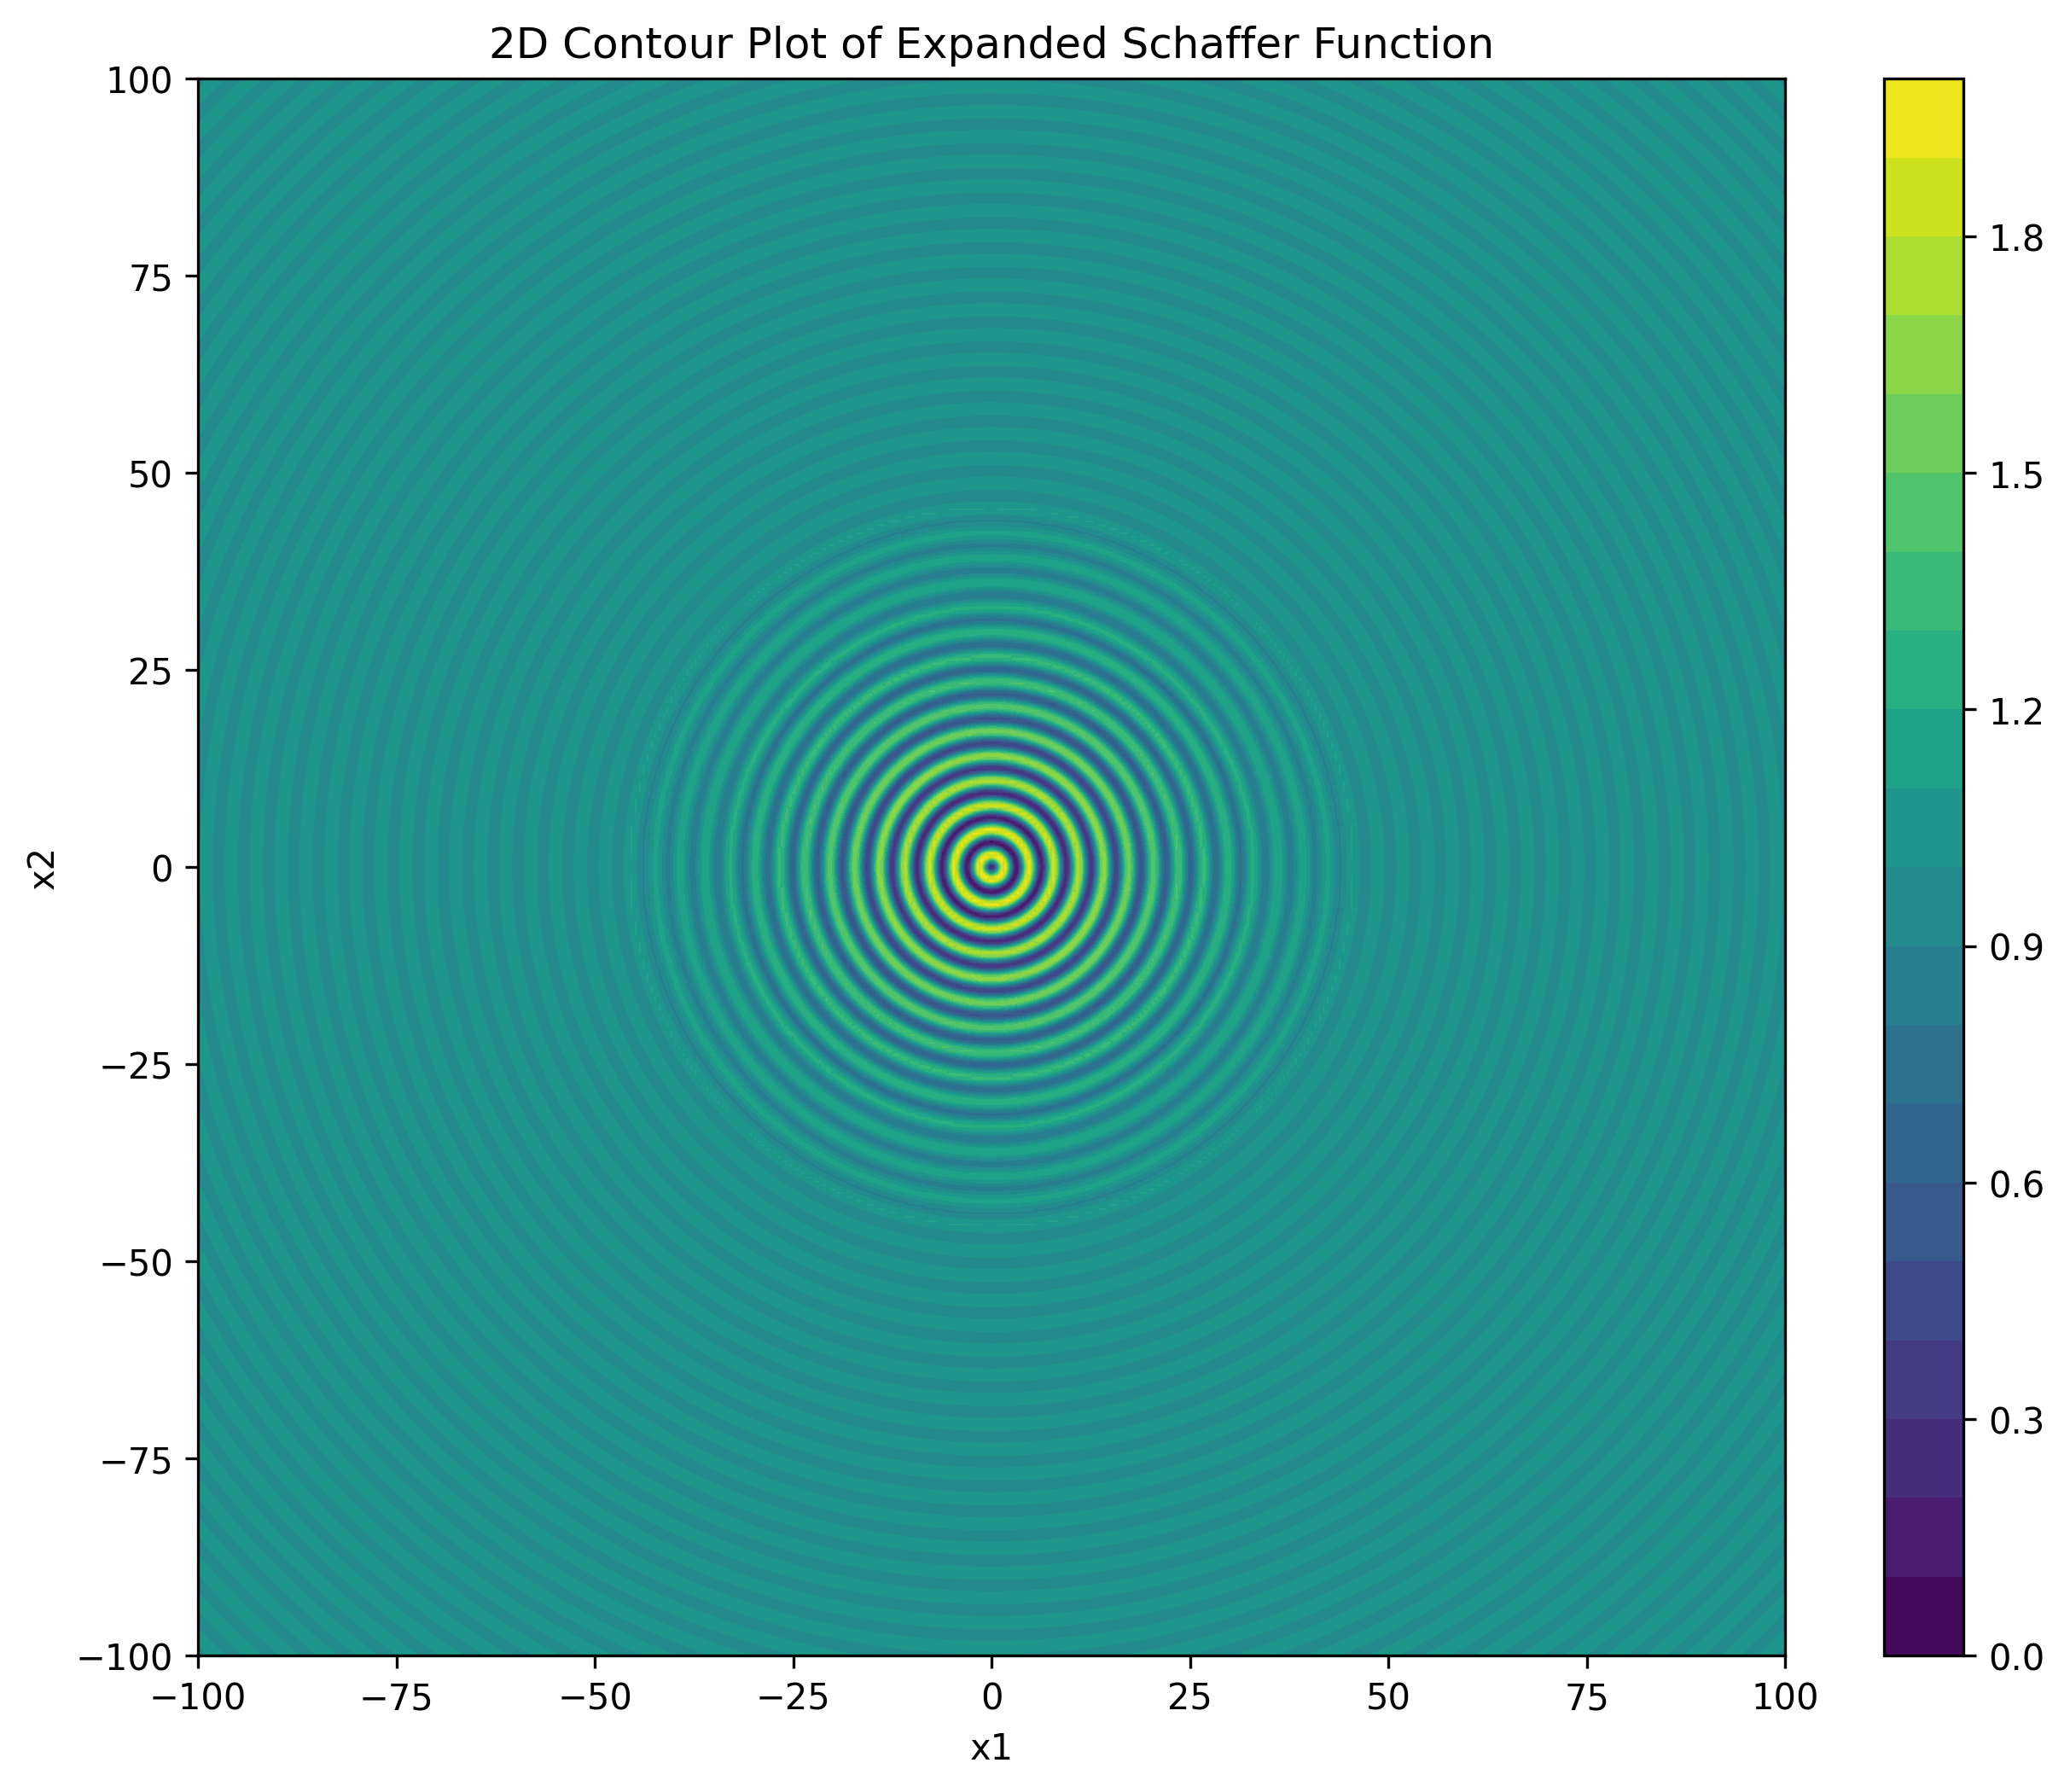
\includegraphics[width=\linewidth]{cec/expanded_schaffer_2d.png}
		\caption{Dimensi 2}
		\label{fig:schaffer-2d}
	\end{subfigure}
	\hfill
	\begin{subfigure}[b]{0.4\textwidth}
		\centering
		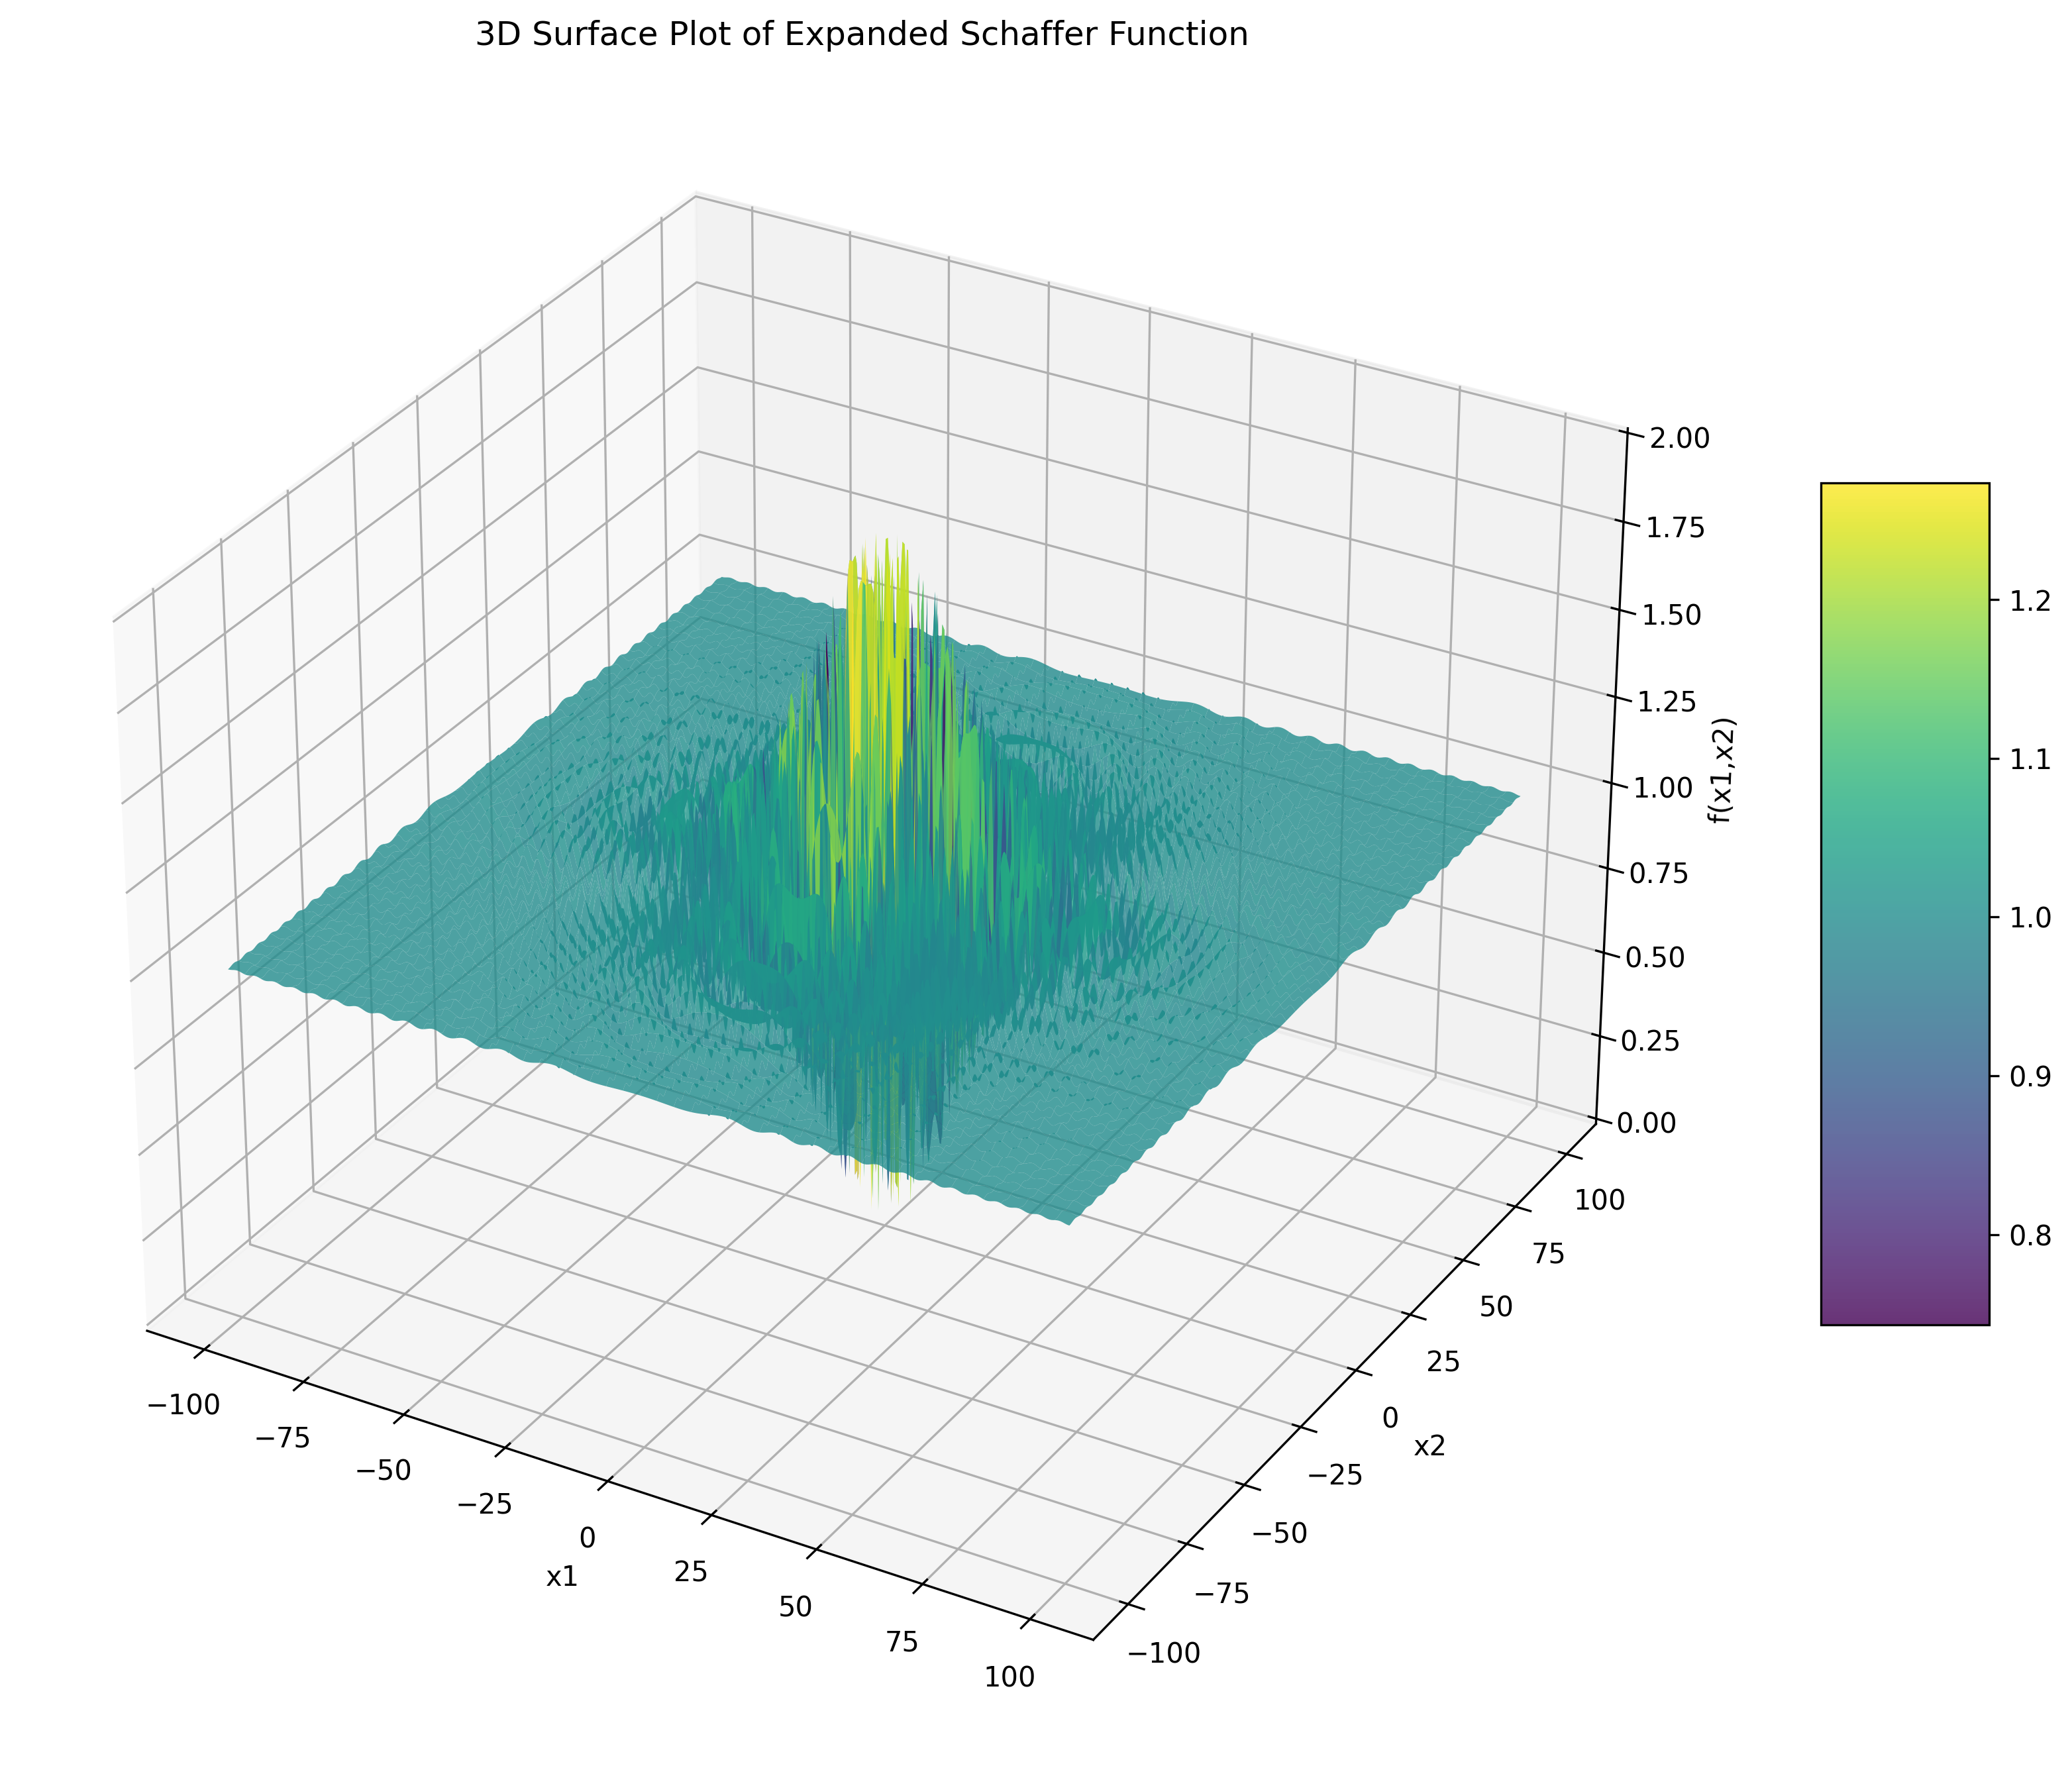
\includegraphics[width=\linewidth]{cec/expanded_schaffer_3d.png}
		\caption{Dimensi 3}
		\label{fig:schaffer-3d}
	\end{subfigure}
	\caption{Tampilan grafik fungsi Expanded schaffer f6 pada dimensi dua (\cref{fig:schaffer-2d}) dan tiga (\cref{fig:schaffer-3d})}
	\label{fig:schaffer}
\end{figure}
\begin{equation}
  \begin{split}
    g\left(x,y \right) &= 0.5+\frac{\sin^2\left(\sqrt{x^2+y^2} \right)-0.5 }{\left( 1+0.0001\left(x^2+y^2 \right) \right)^2 }\\
    f_{\text{Expanded schaffer f6}}(\mathrm{x}) &= g\left(z_1,z_2 \right)+\cdots+g\left(z_D,z_1 \right)+f_{\text{bias}}
  \end{split}
\end{equation}

\subsubsection*{Griewank}
\noindent Properti:
\begin{packed_item}
  \item multimodal
  \item non-convex
  \item non-separable
  \item scalable
\end{packed_item}
\begin{figure}[H]
	\centering
	\begin{subfigure}[b]{0.4\textwidth}
		\centering
		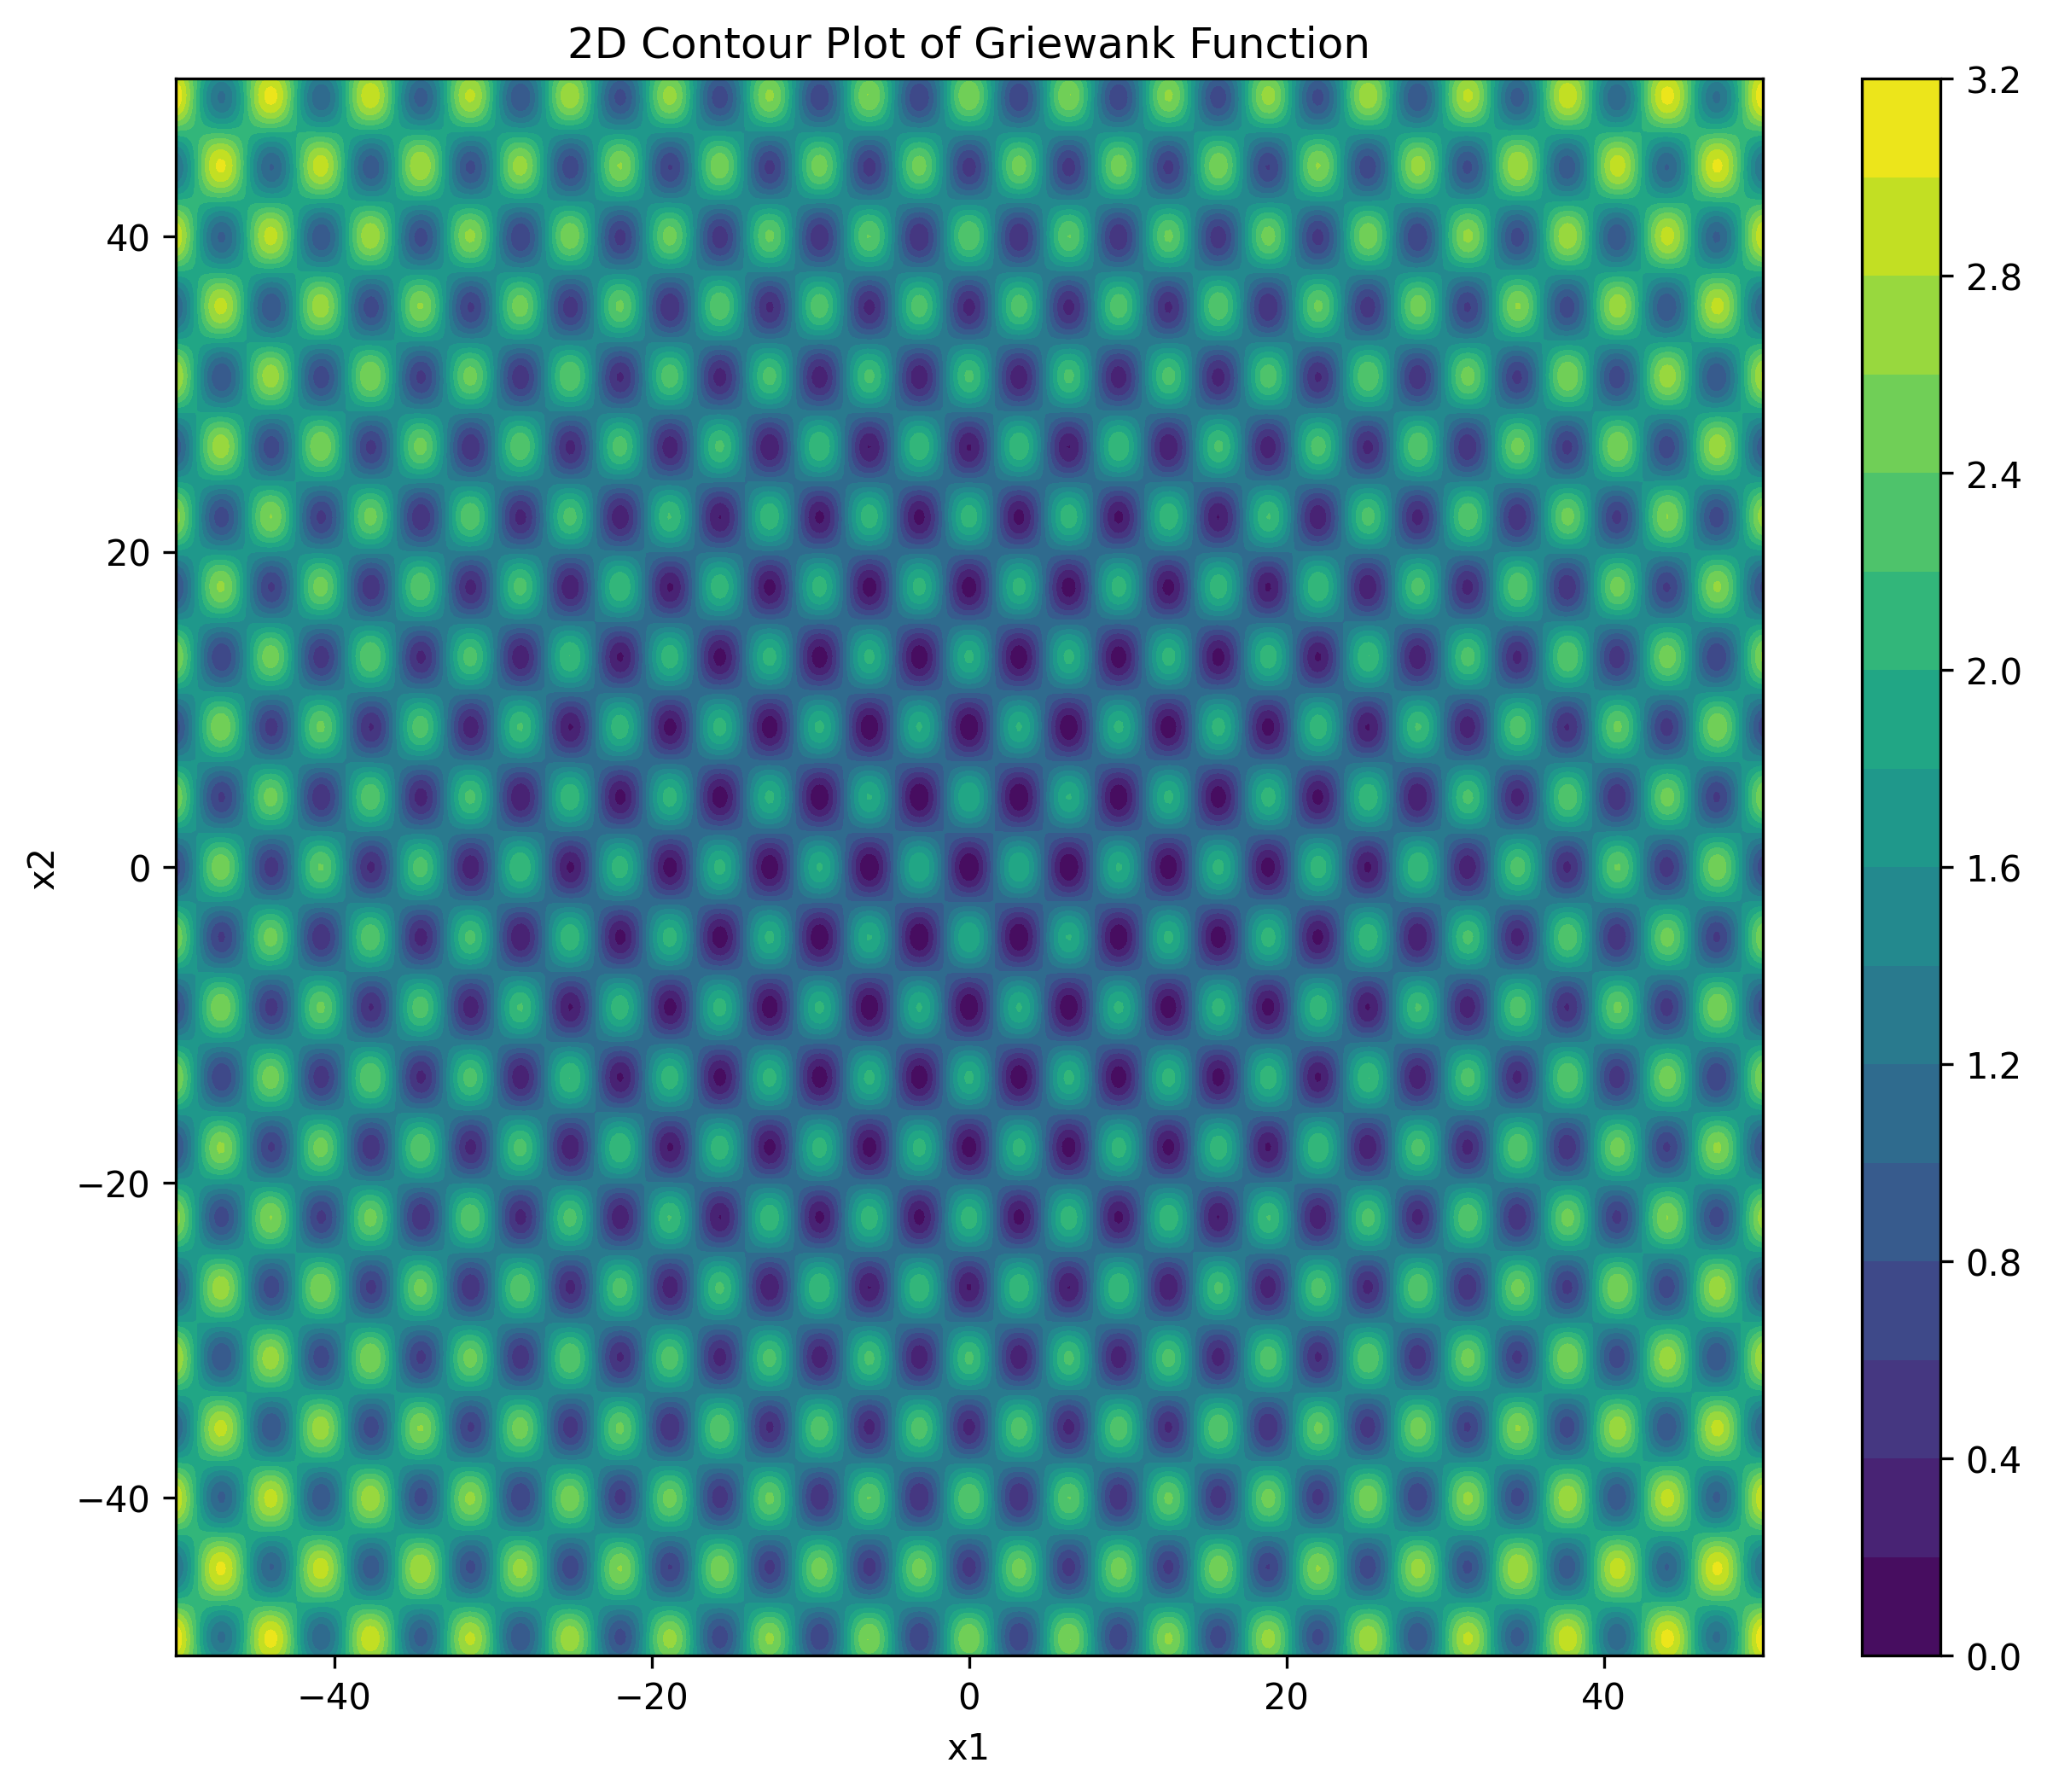
\includegraphics[width=\linewidth]{cec/griewank_2d.png}
		\caption{Dimensi 2}
		\label{fig:griewank-2d}
	\end{subfigure}
	\hfill
	\begin{subfigure}[b]{0.4\textwidth}
		\centering
		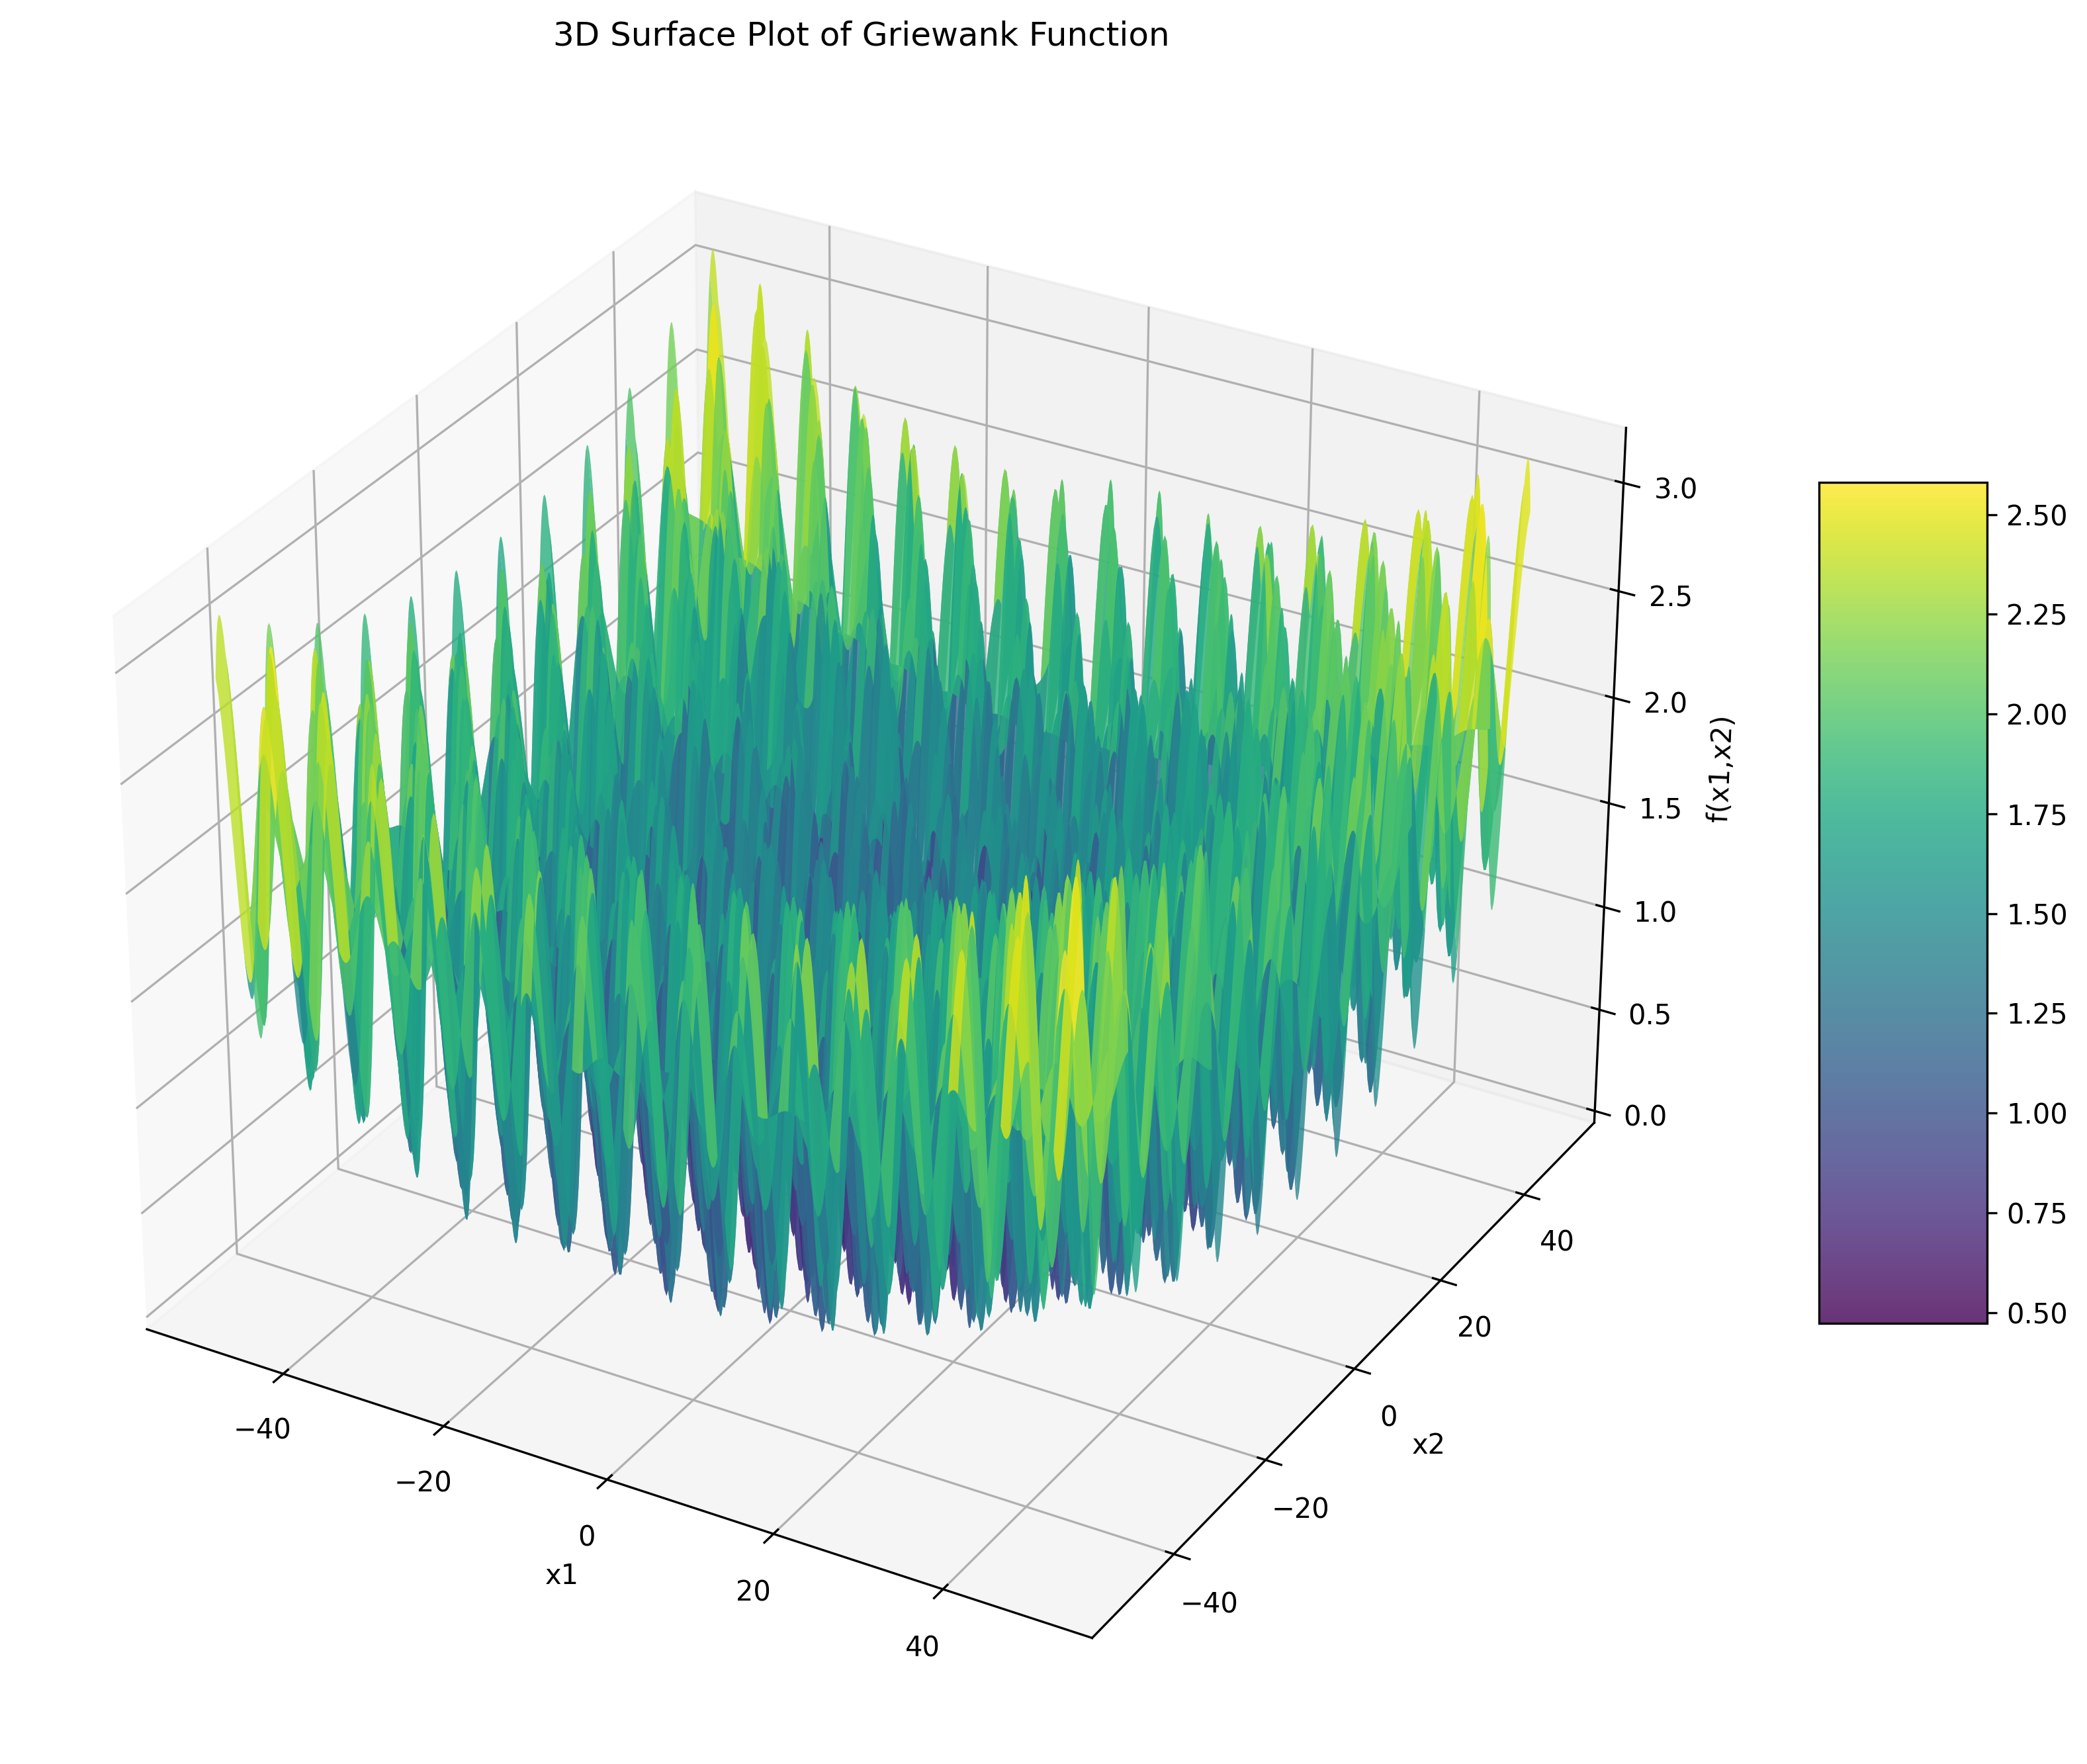
\includegraphics[width=\linewidth]{cec/griewank_3d.png}
		\caption{Dimensi 3}
		\label{fig:griewank-3d}
	\end{subfigure}
	\caption{Tampilan grafik fungsi Griewank pada dimensi dua (\cref{fig:griewank-2d}) dan tiga (\cref{fig:griewank-3d})}
	\label{fig:griewank}
\end{figure}
\begin{equation}
  f_{\text{Griewank}}(\mathrm{x})=\sum_{i=1}^{D}\frac{z_i^2}{4000}-\prod_{i=1}^{D}\cos\left( \frac{z_i}{\sqrt{i}}\right)+1 +f_{\text{bias}}
\end{equation}

\subsubsection*{Happycat}
\noindent Properti:
\begin{packed_item}
  \item multimodal
  \item non-convex
  \item non-separable
\end{packed_item}
\begin{figure}[H]
	\centering
	\begin{subfigure}[b]{0.4\textwidth}
		\centering
		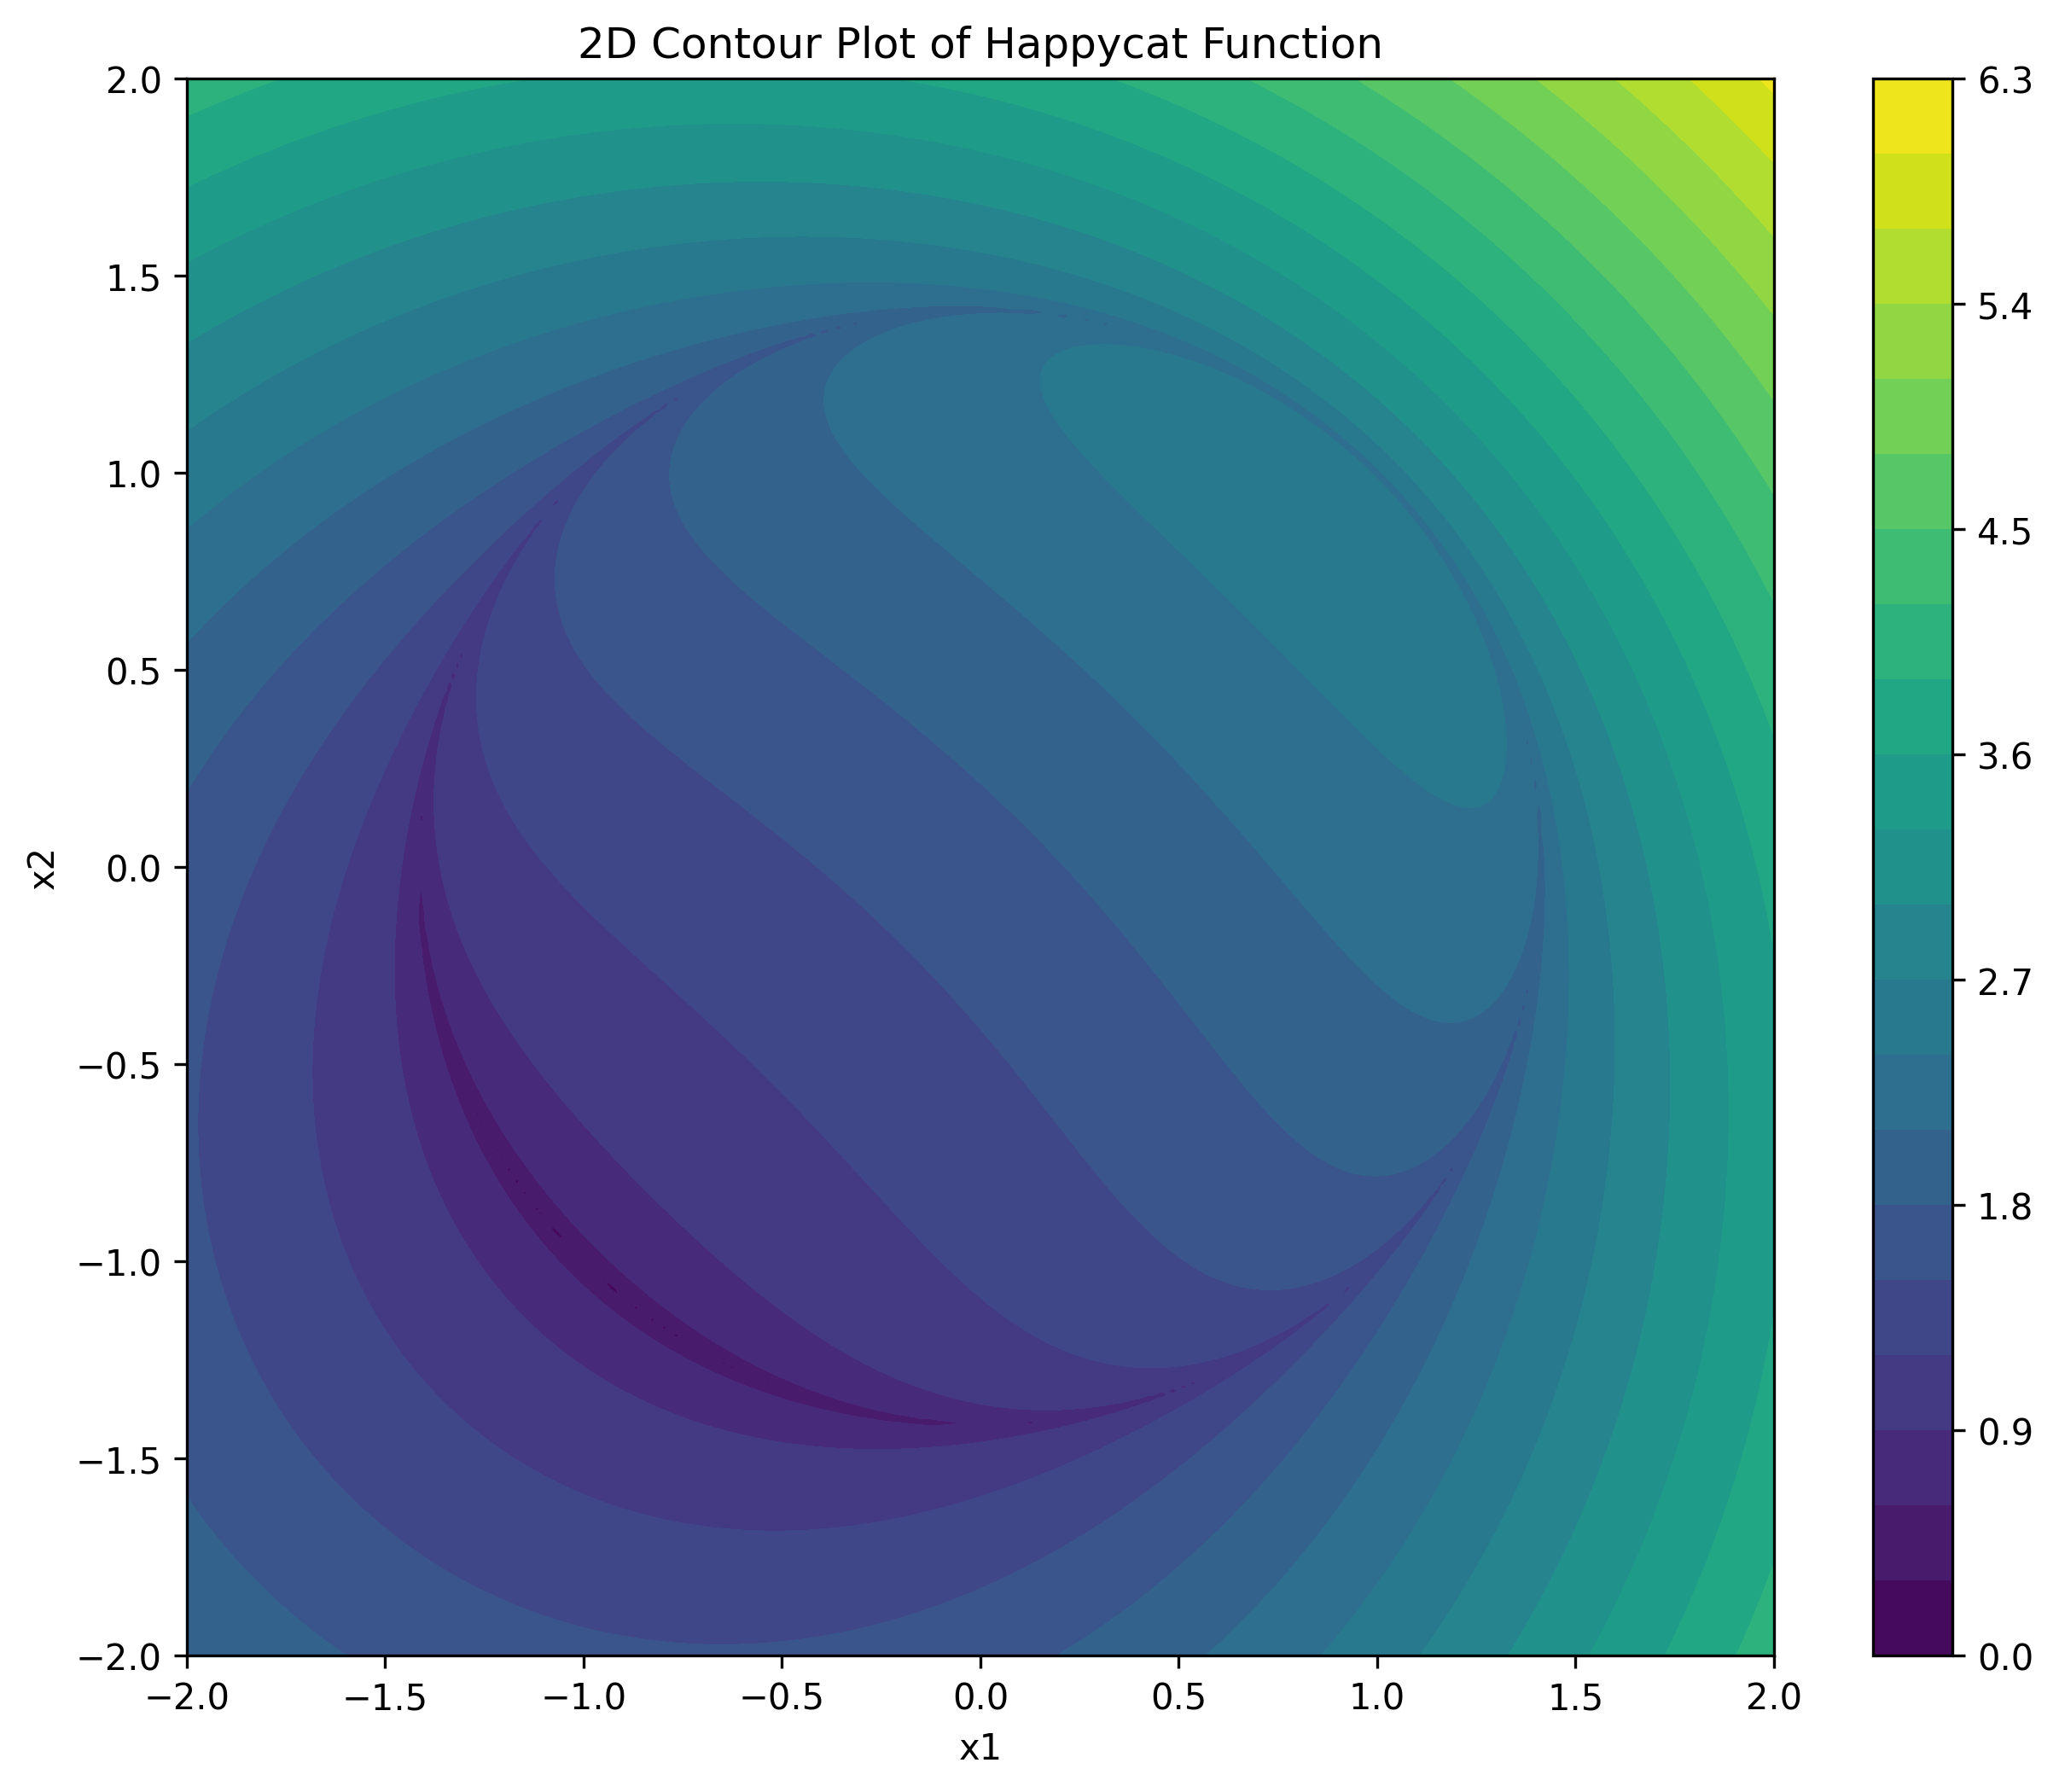
\includegraphics[width=\linewidth]{cec/happycat_2d.png}
		\caption{Dimensi 2}
		\label{fig:happycat-2d}
	\end{subfigure}
	\hfill
	\begin{subfigure}[b]{0.4\textwidth}
		\centering
		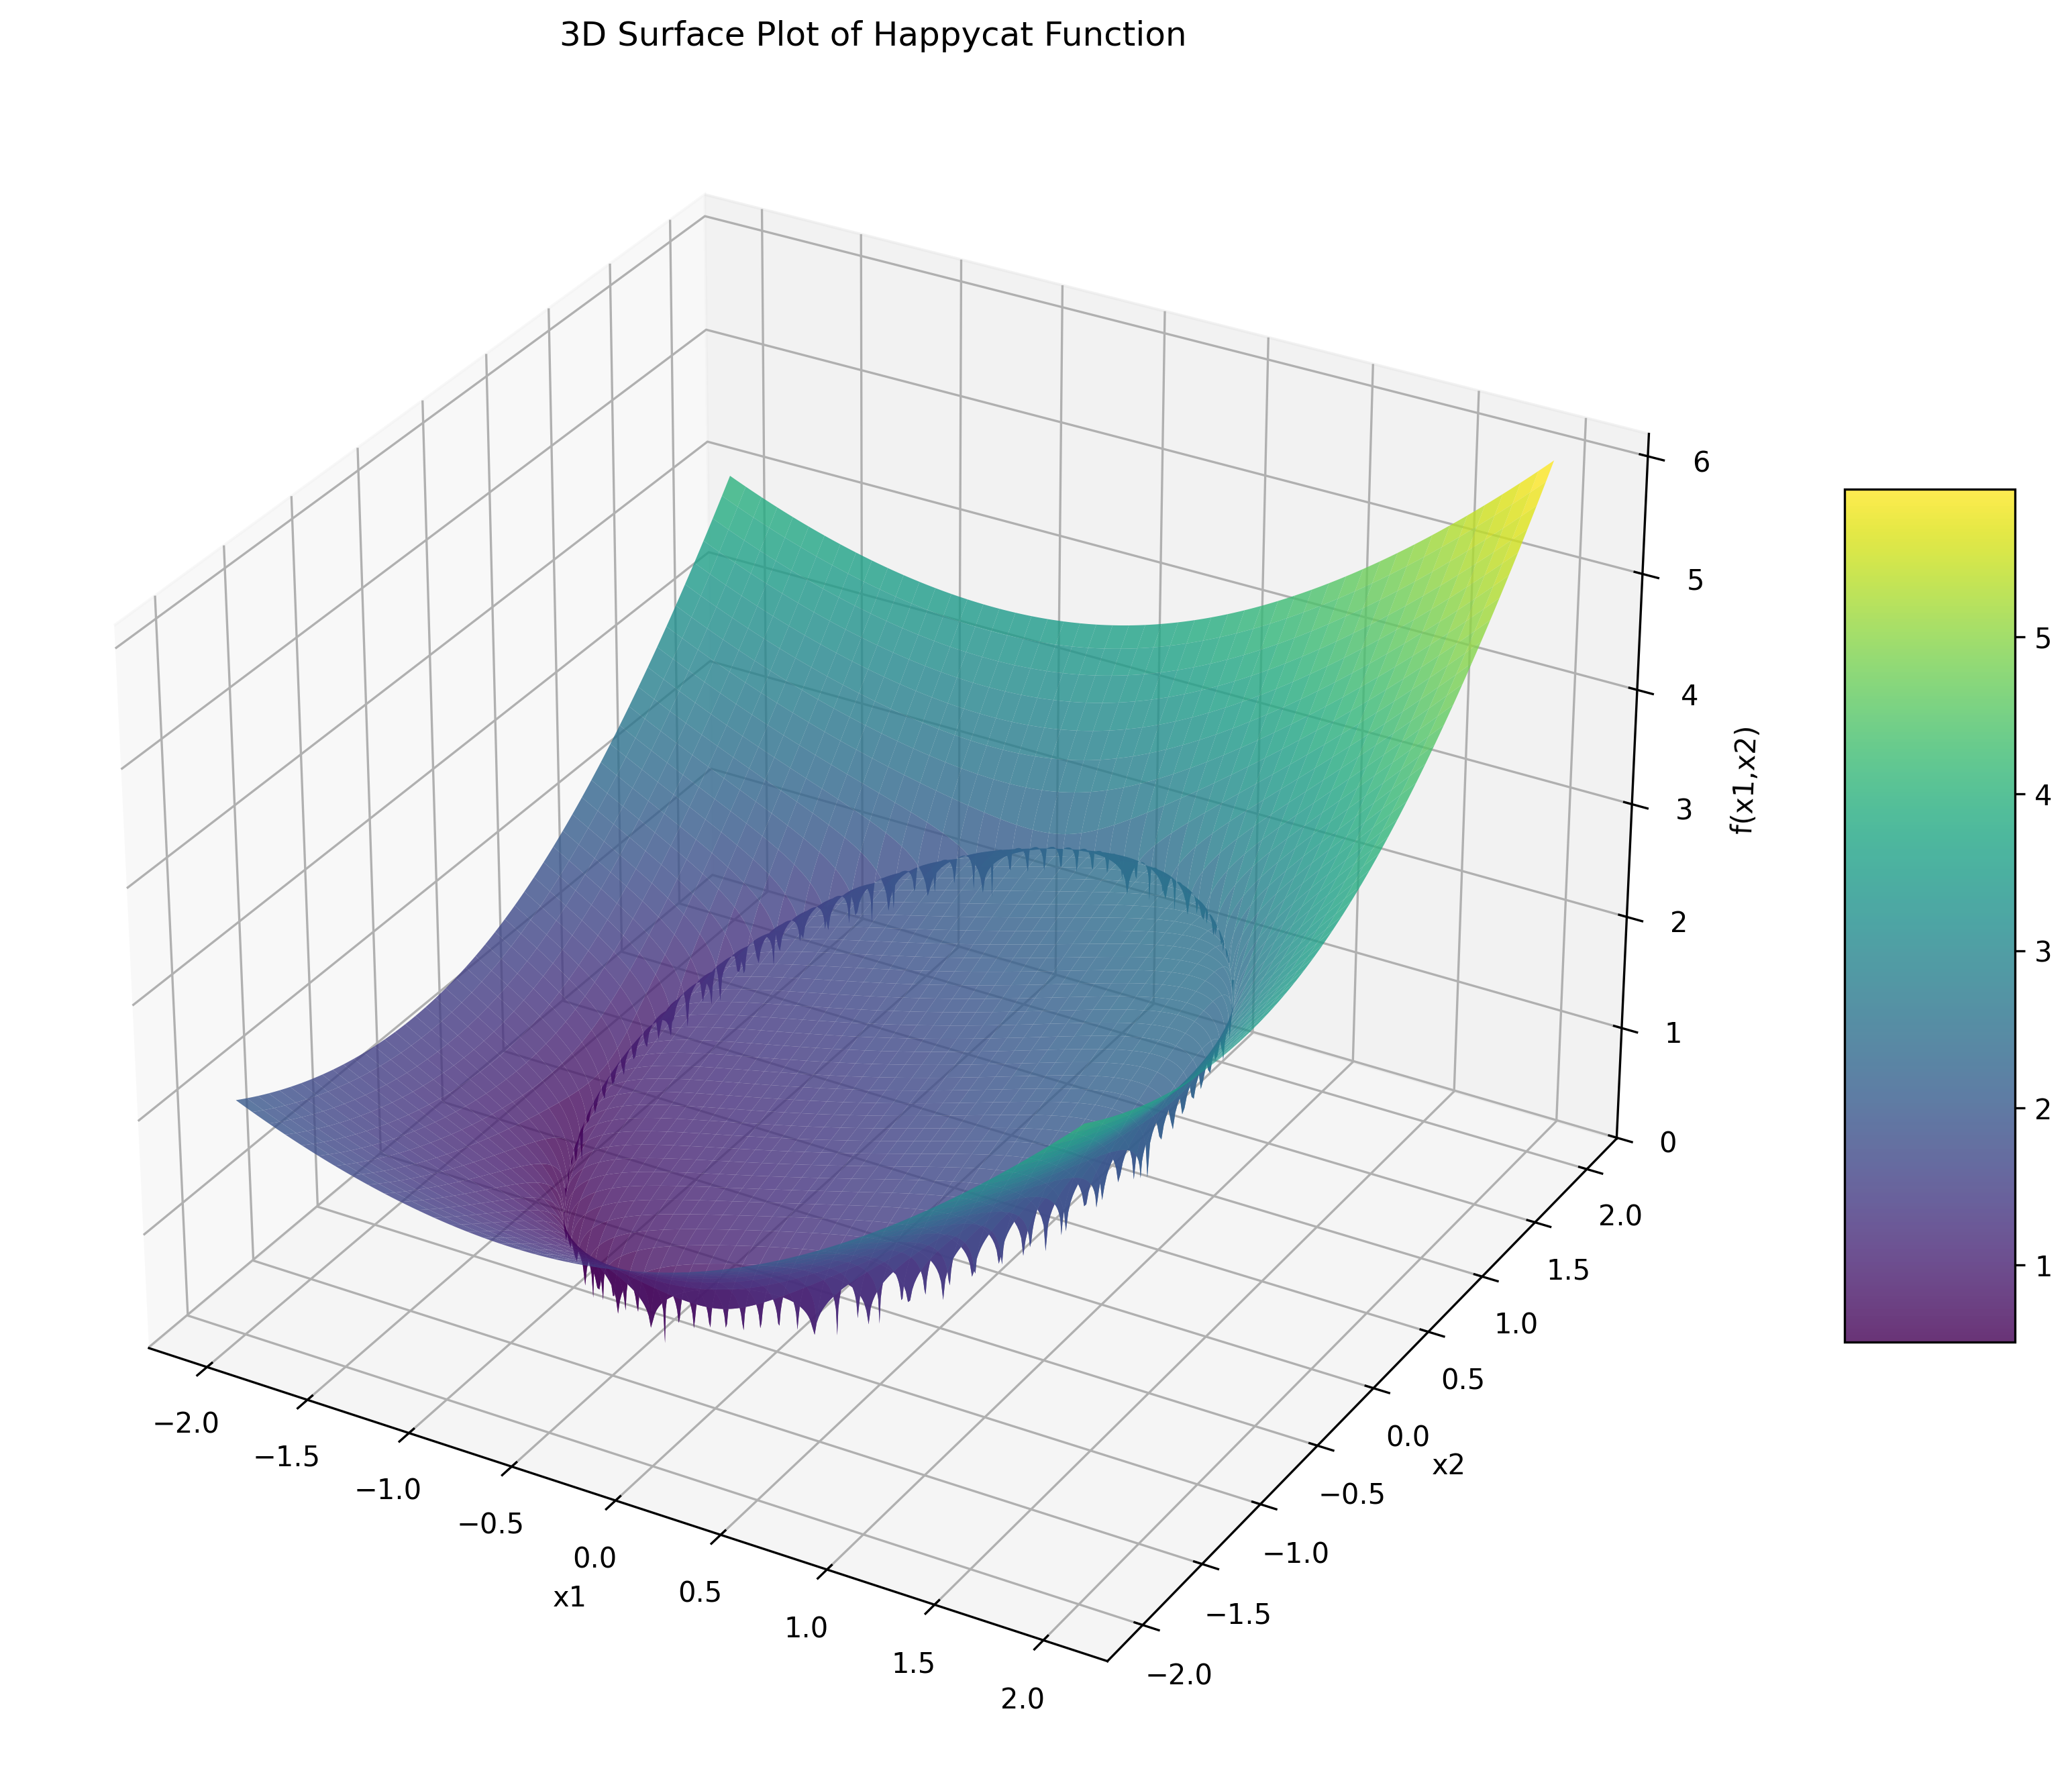
\includegraphics[width=\linewidth]{cec/happycat_3d.png}
		\caption{Dimensi 3}
		\label{fig:happycat-3d}
	\end{subfigure}
	\caption{Tampilan grafik fungsi Happycat pada dimensi dua (\cref{fig:happycat-2d}) dan tiga (\cref{fig:happycat-3d})}
	\label{fig:happycat}
\end{figure}
\begin{equation}
  f_{\text{Happycat}}(\mathrm{x})=\left|\sum_{i=1}^{D}z_i^2-D \right|^{1/4}+\left(0.5\sum_{i=1}^{D}z_i+\sum_{i=1}^{D}z_i \right)/D+0.5+f_{\text{bias}}
\end{equation}

\subsubsection*{HGbat}
\noindent Properti:
\begin{packed_item}
  \item multimodal
  \item non-convex
  \item non-separable
\end{packed_item}
\begin{figure}[H]
	\centering
	\begin{subfigure}[b]{0.4\textwidth}
		\centering
		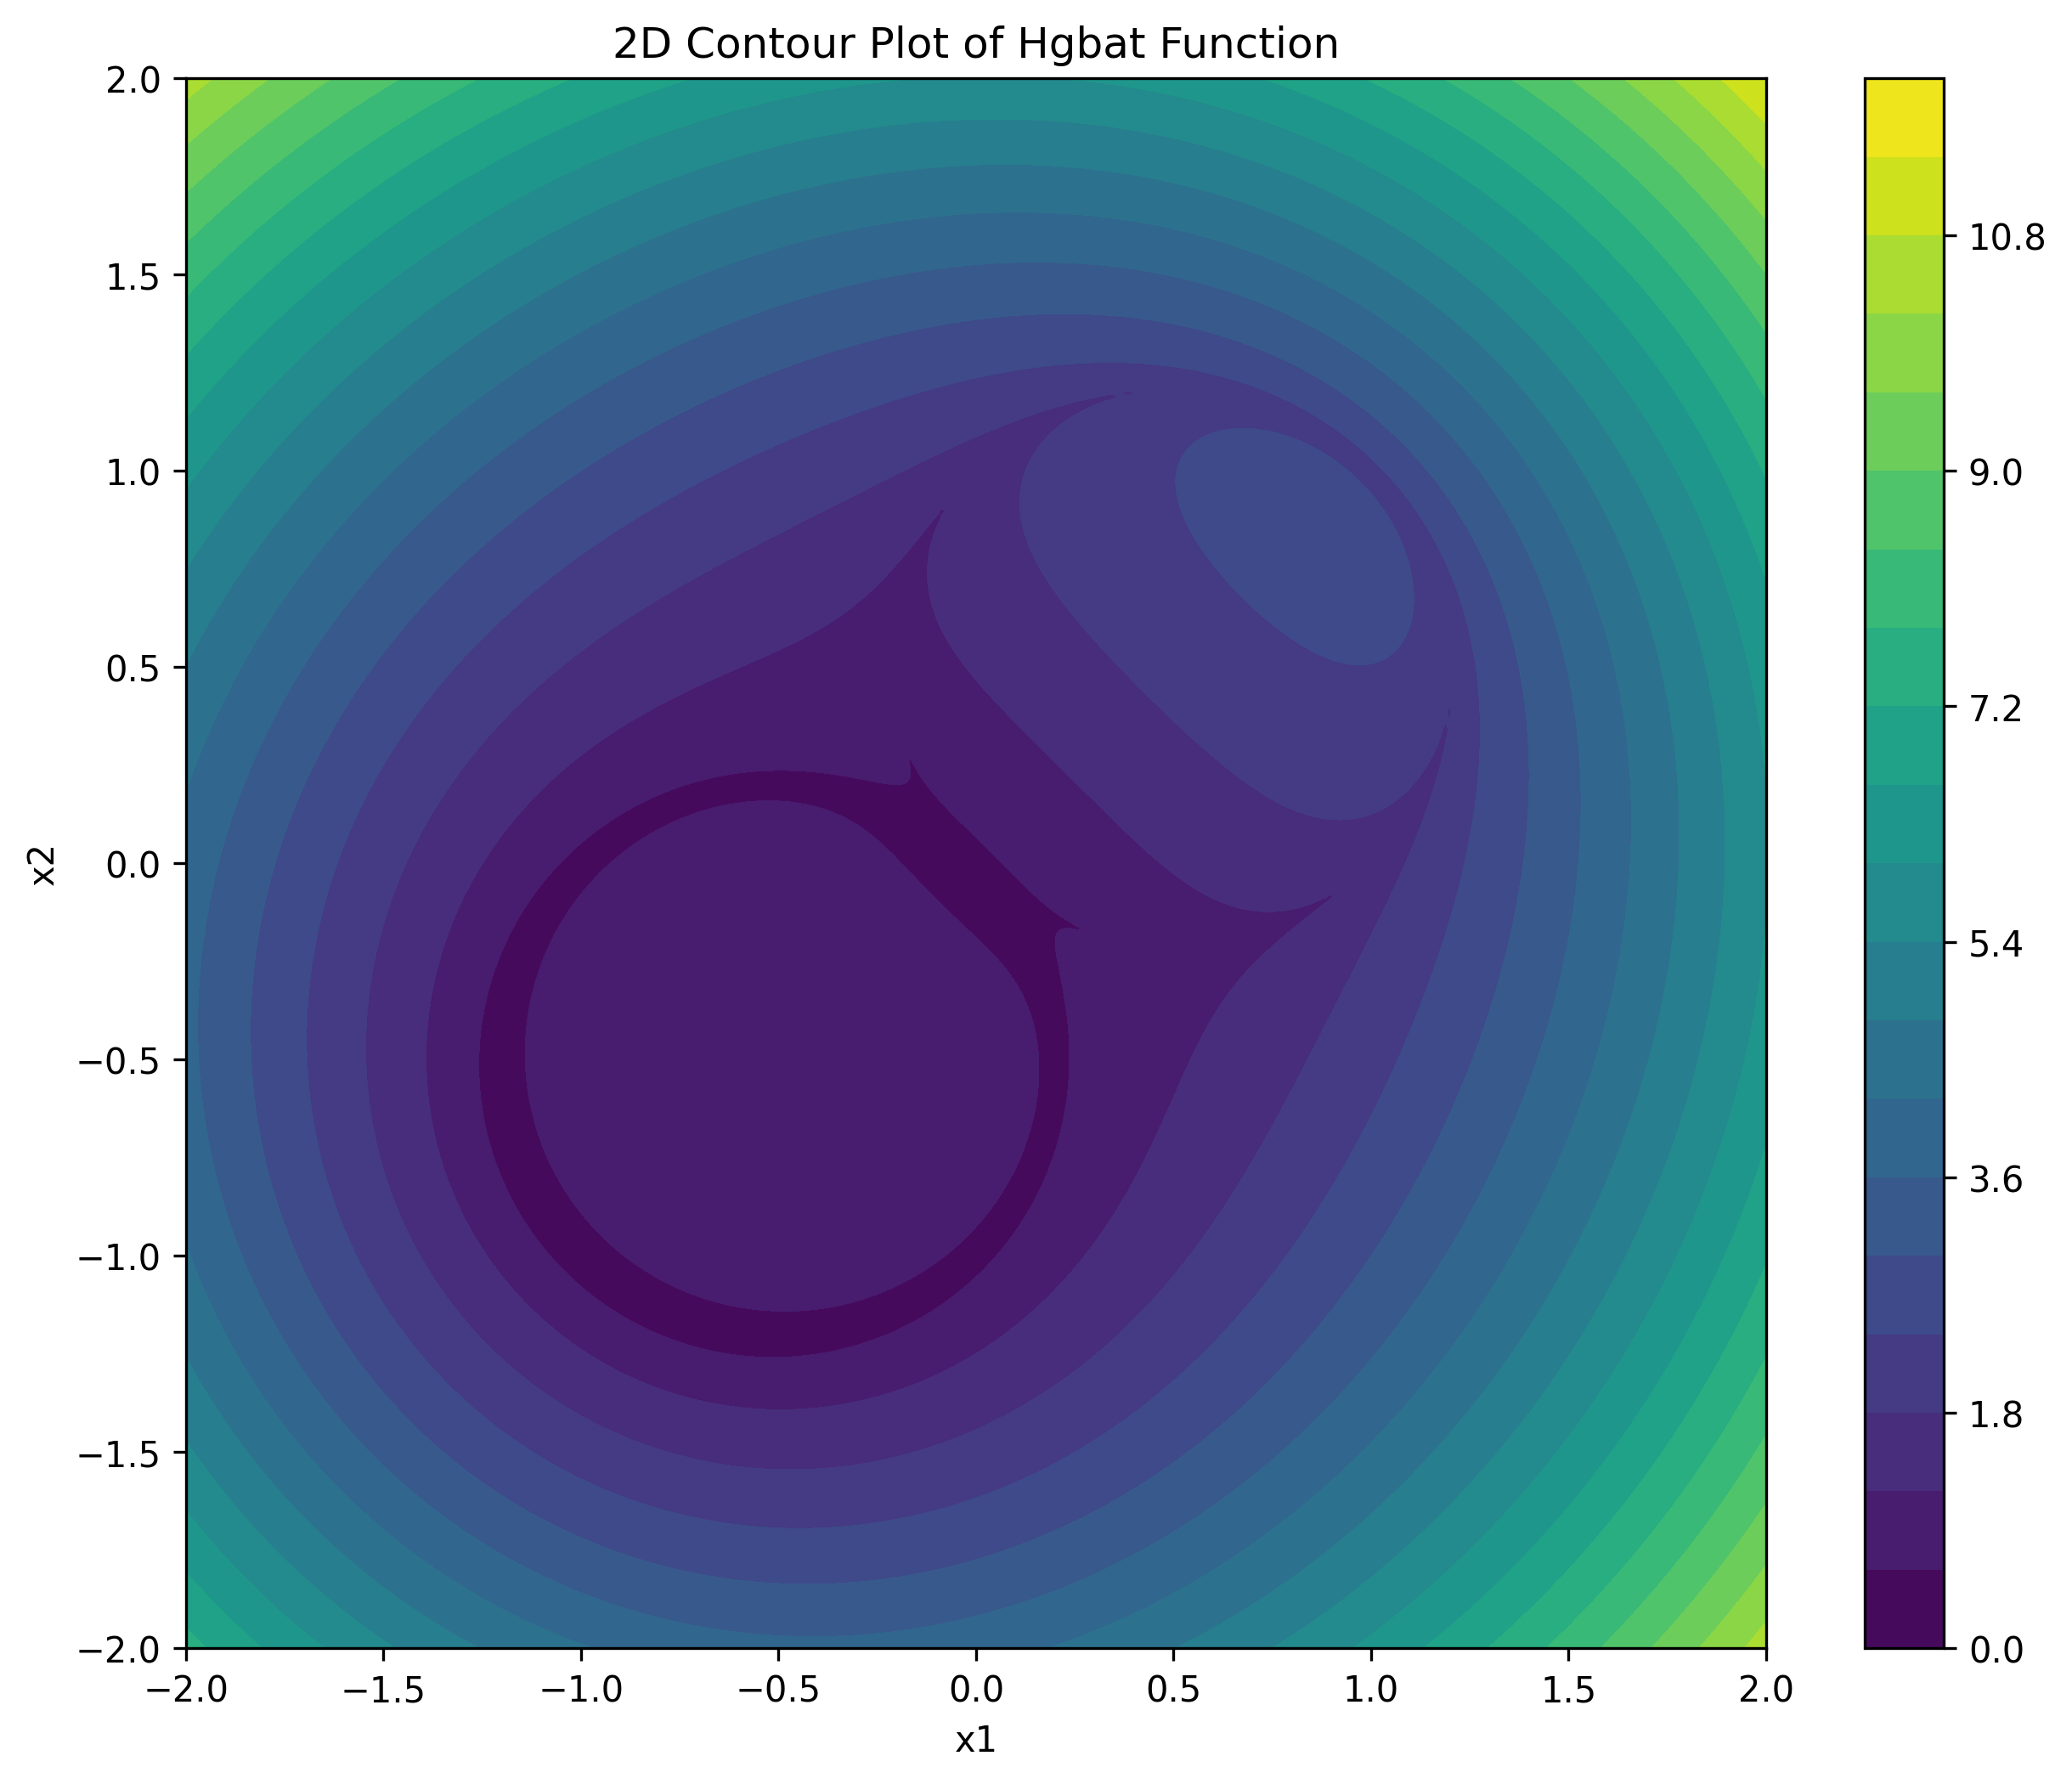
\includegraphics[width=\linewidth]{cec/hgbat_2d.png}
		\caption{Dimensi 2}
		\label{fig:hgbat-2d}
	\end{subfigure}
	\hfill
	\begin{subfigure}[b]{0.4\textwidth}
		\centering
		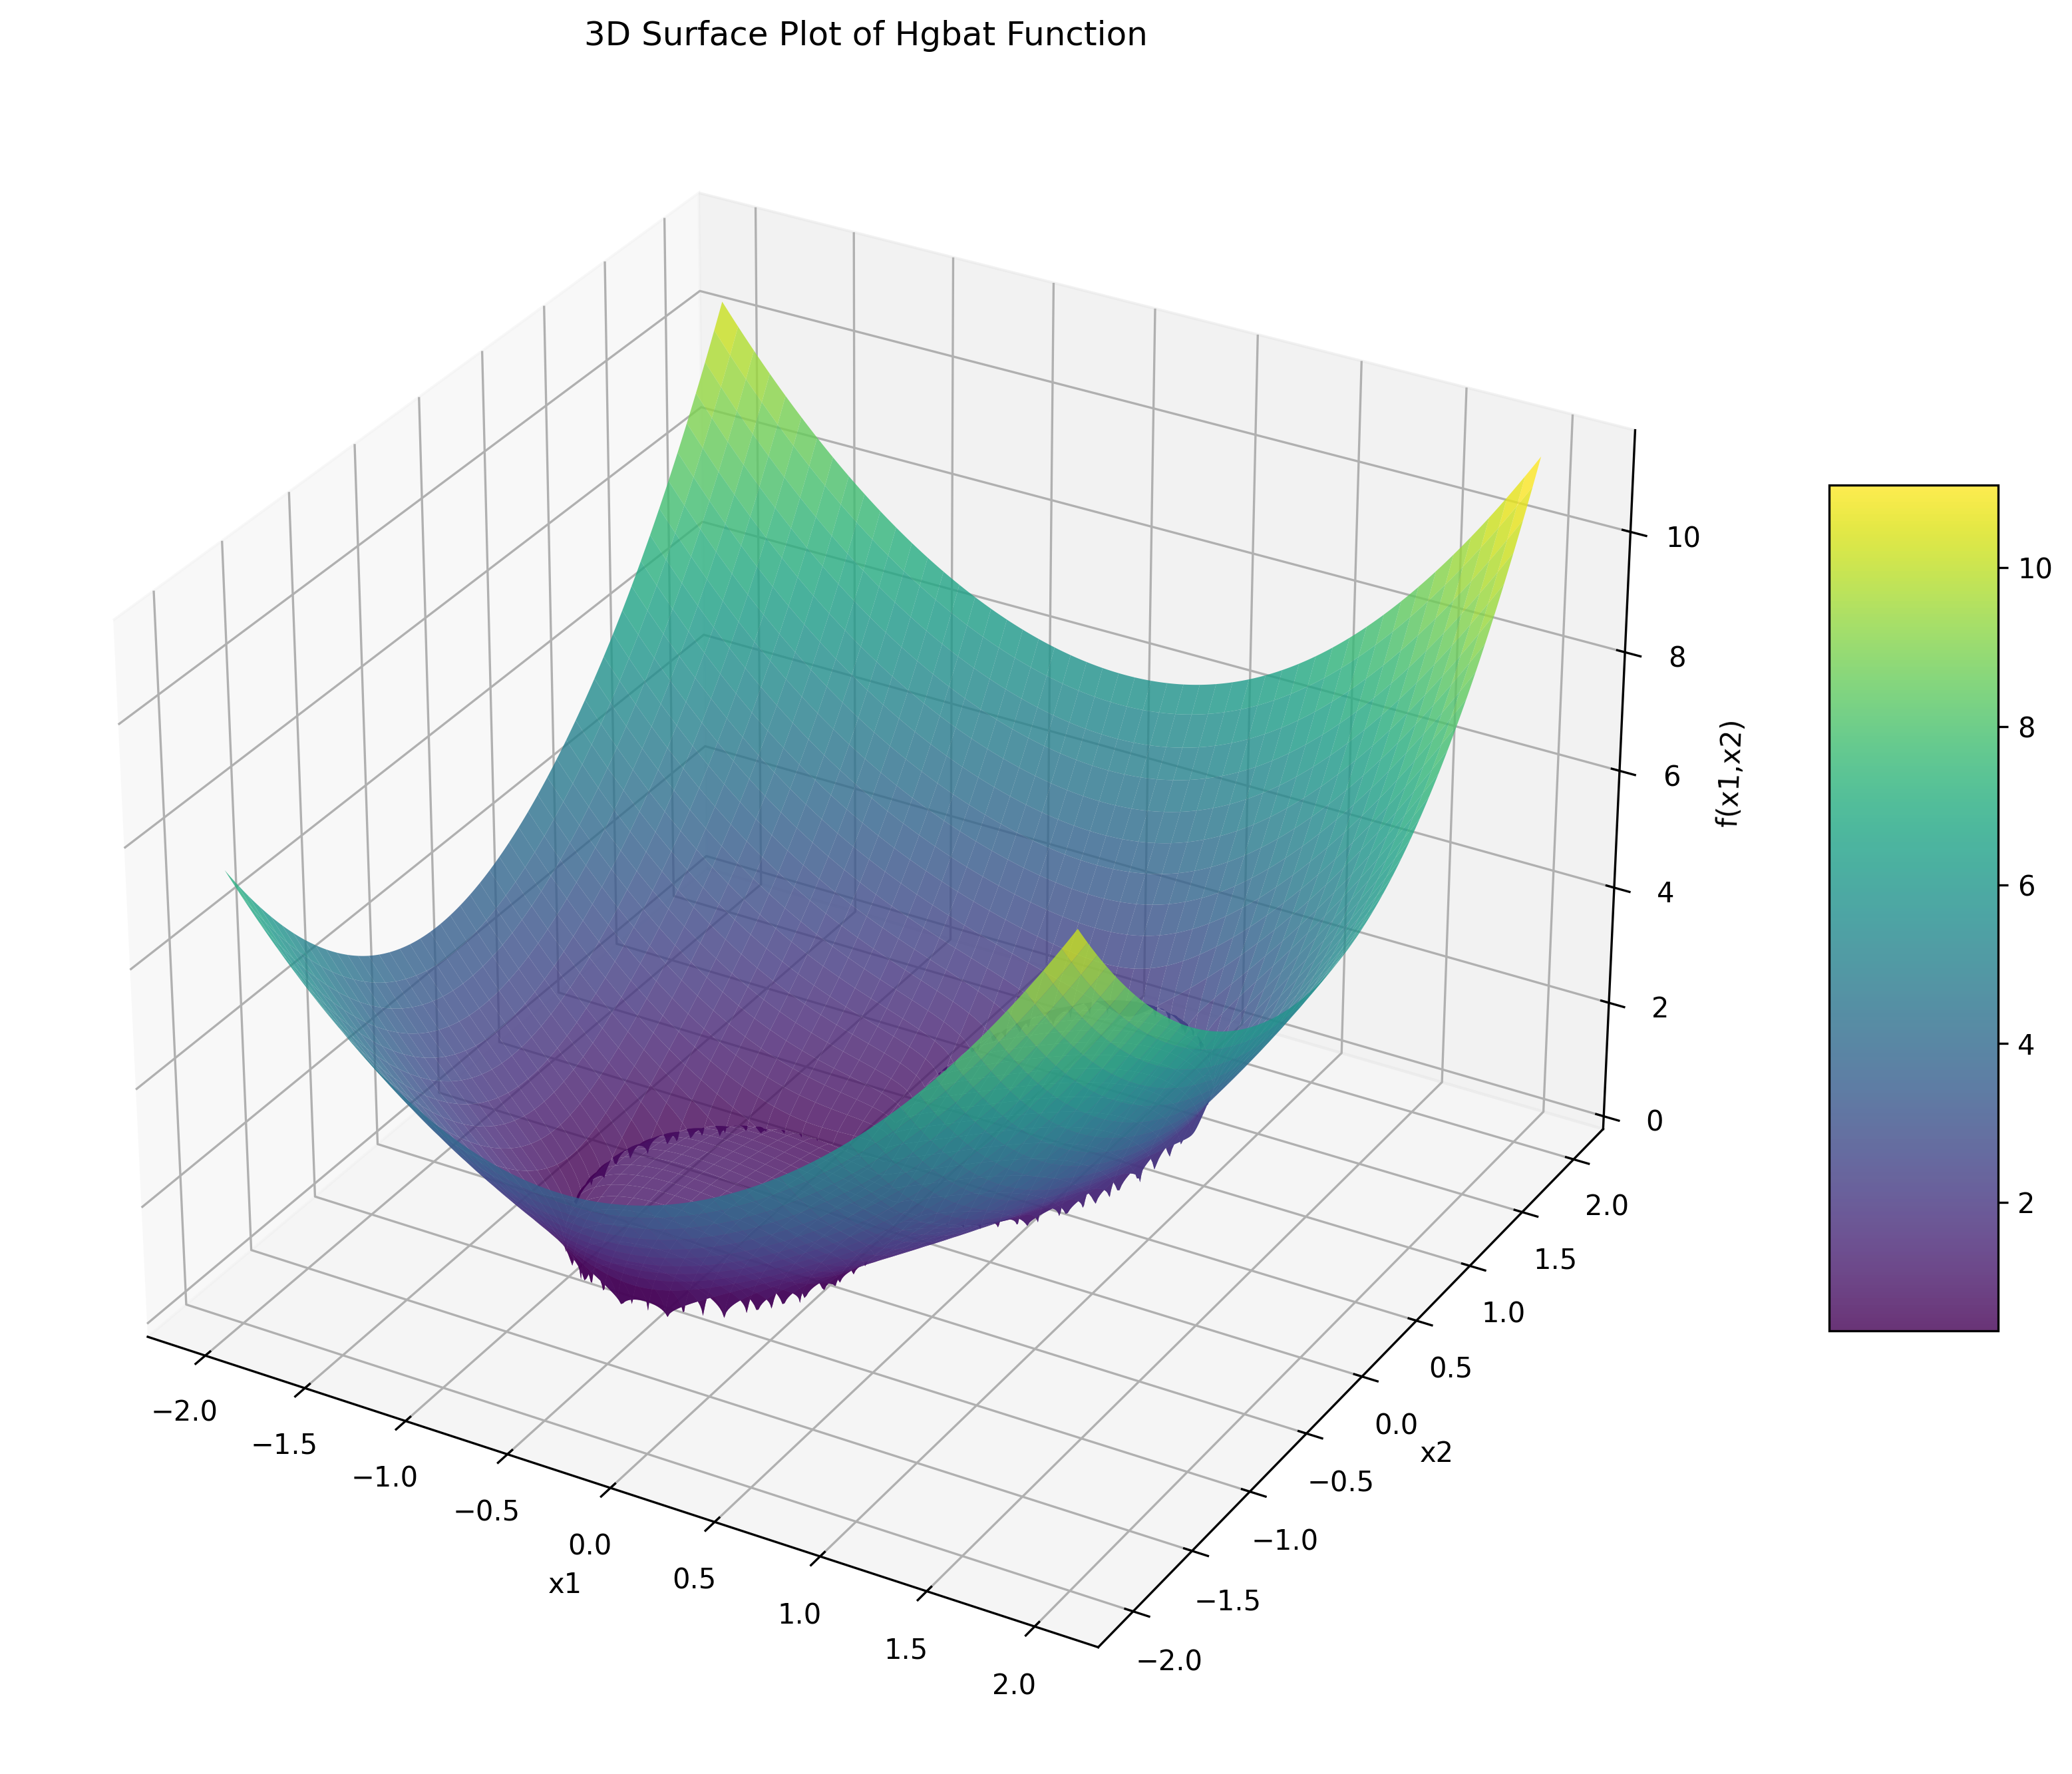
\includegraphics[width=\linewidth]{cec/hgbat_3d.png}
		\caption{Dimensi 3}
		\label{fig:hgbat-3d}
	\end{subfigure}
	\caption{Tampilan grafik fungsi HGbat pada dimensi dua (\cref{fig:hgbat-2d}) dan tiga (\cref{fig:hgbat-3d})}
	\label{fig:hgbat}
\end{figure}
\begin{equation}
  f_{\text{HGbat}}(\mathrm{x})=\left|\left( \sum_{i=1}^{D}z_i^2\right)^2-\left(\sum_{i=1}^{D}z_i \right)^2  \right|^{1/2}+\left(0.5\sum_{i=1}^{D}z_i+\sum_{i=1}^{D}z_i \right)/D+0.5+f_{\text{bias}}
\end{equation}

\subsubsection*{Katsuura}
\noindent Properti:
\begin{packed_item}
  \item multimodal
  \item non-convex
  \item non-separable
  \item Continuous everywhere yet differentiable nowhere
\end{packed_item}
\begin{figure}[H]
	\centering
	\begin{subfigure}[b]{0.4\textwidth}
		\centering
		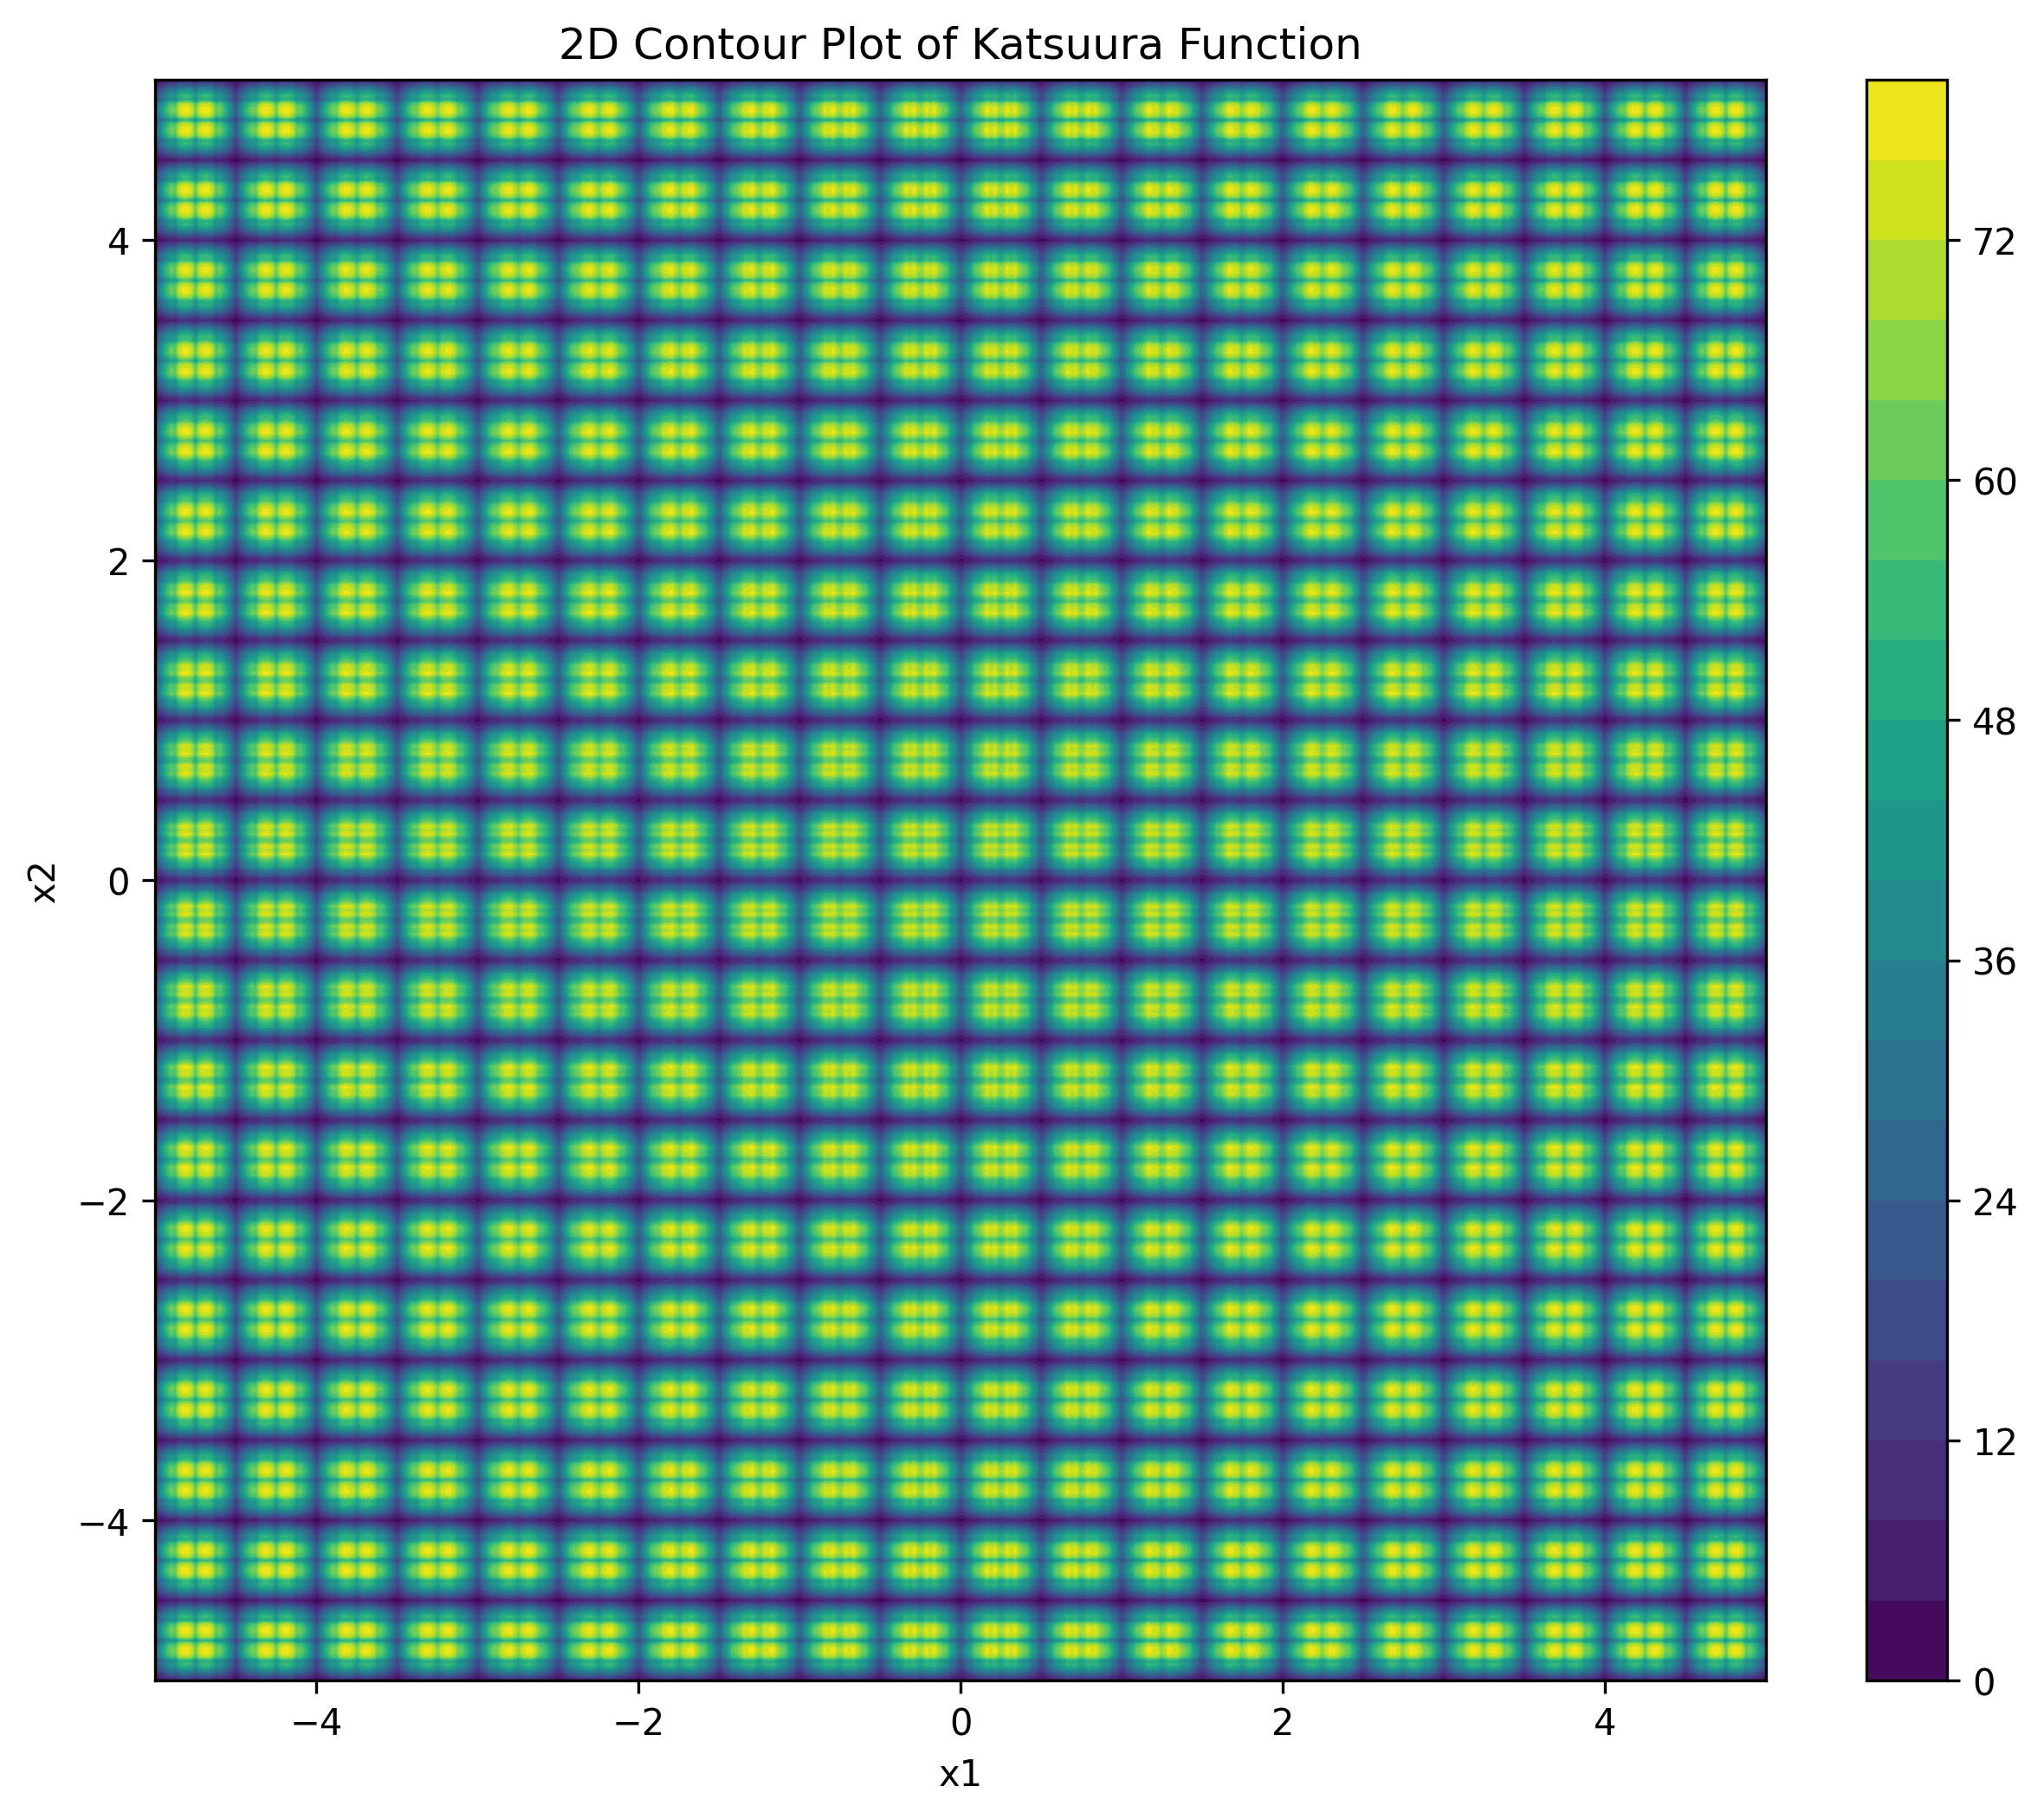
\includegraphics[width=\linewidth]{cec/katsuura_2d.png}
		\caption{Dimensi 2}
		\label{fig:katsuura-2d}
	\end{subfigure}
	\hfill
	\begin{subfigure}[b]{0.4\textwidth}
		\centering
		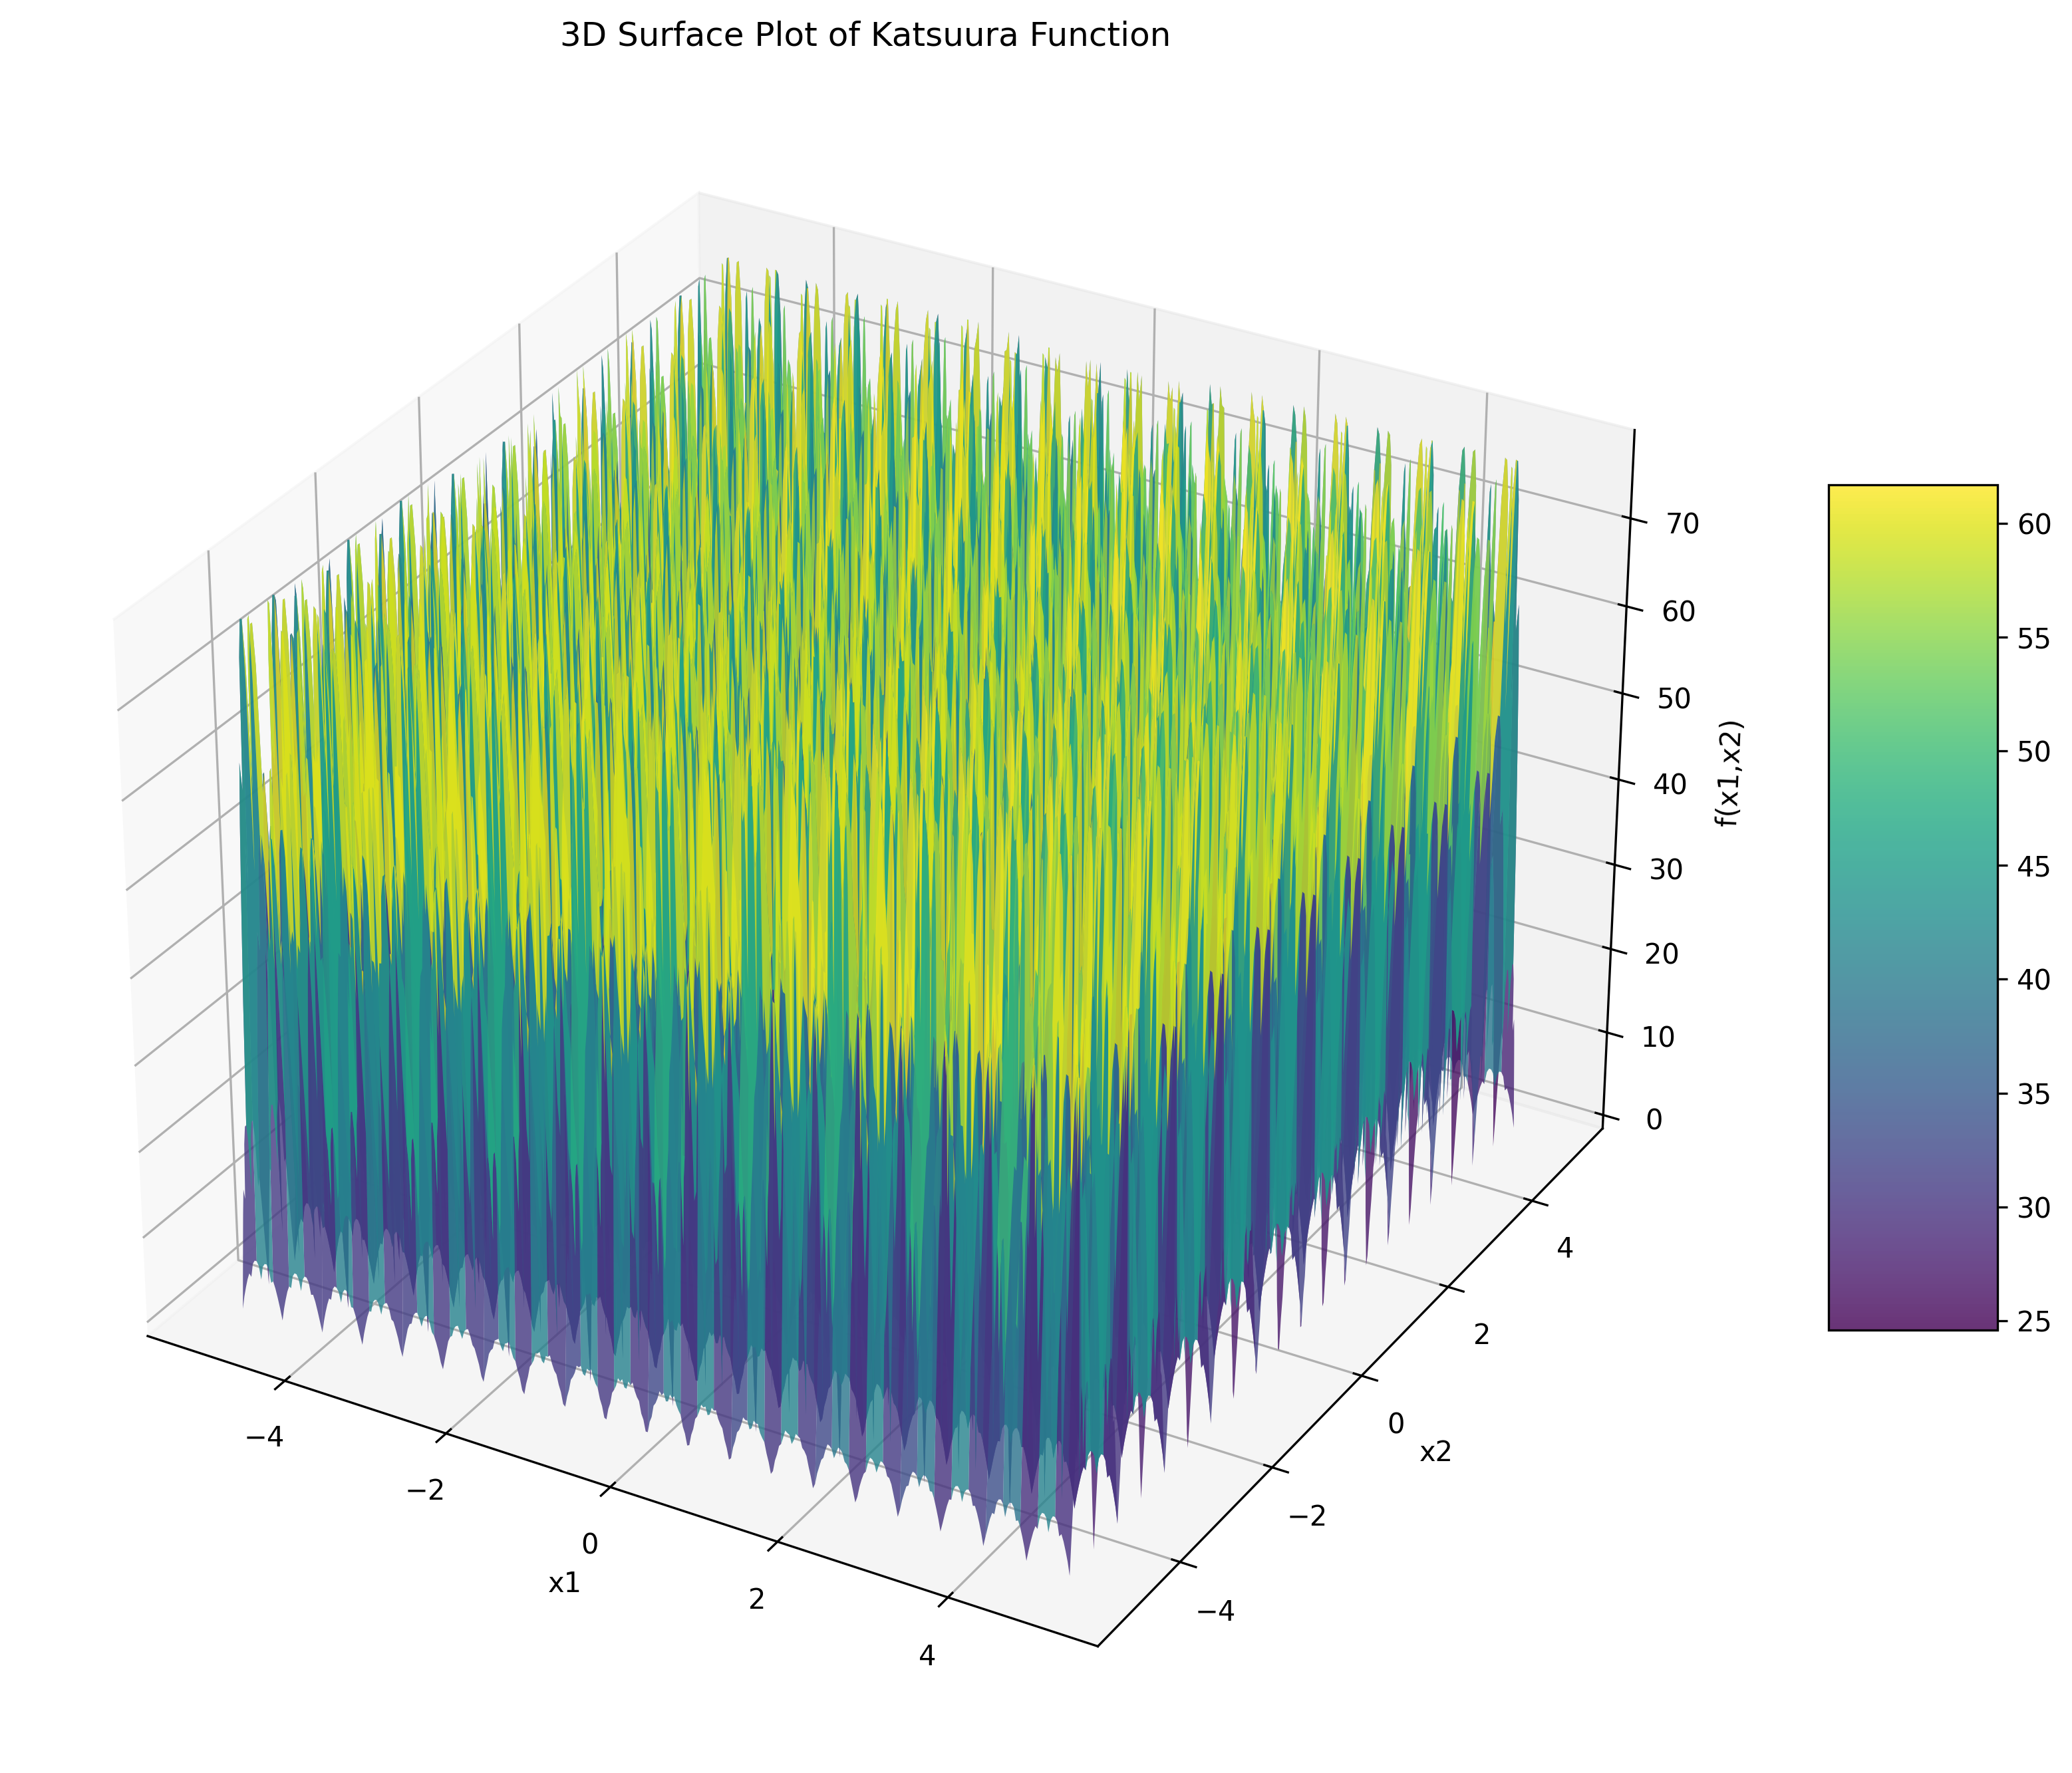
\includegraphics[width=\linewidth]{cec/katsuura_3d.png}
		\caption{Dimensi 3}
		\label{fig:katsuura-3d}
	\end{subfigure}
	\caption{Tampilan grafik fungsi Katsuura pada dimensi dua (\cref{fig:katsuura-2d}) dan tiga (\cref{fig:katsuura-3d})}
	\label{fig:katsuura}
\end{figure}
\begin{equation}
  f_{\text{Katsuura}}(\mathrm{x})=\frac{10}{D^2}\prod_{i=1}^{D}\left( 1+i\sum_{j=1}^{32}\frac{\left|2^j z_i-\text{round}\left( 2^jz_i\right)  \right| }{2^j}\right)^{\frac{10}{D^{1.2}}}+f_{\text{bias}}
\end{equation}

\subsubsection*{Levy}
\noindent Properti:
\begin{packed_item}
  \item multimodal
  \item non-convex
  \item non-separable
  \item Local optima's number is huge
\end{packed_item}
\begin{figure}[H]
	\centering
	\begin{subfigure}[b]{0.4\textwidth}
		\centering
		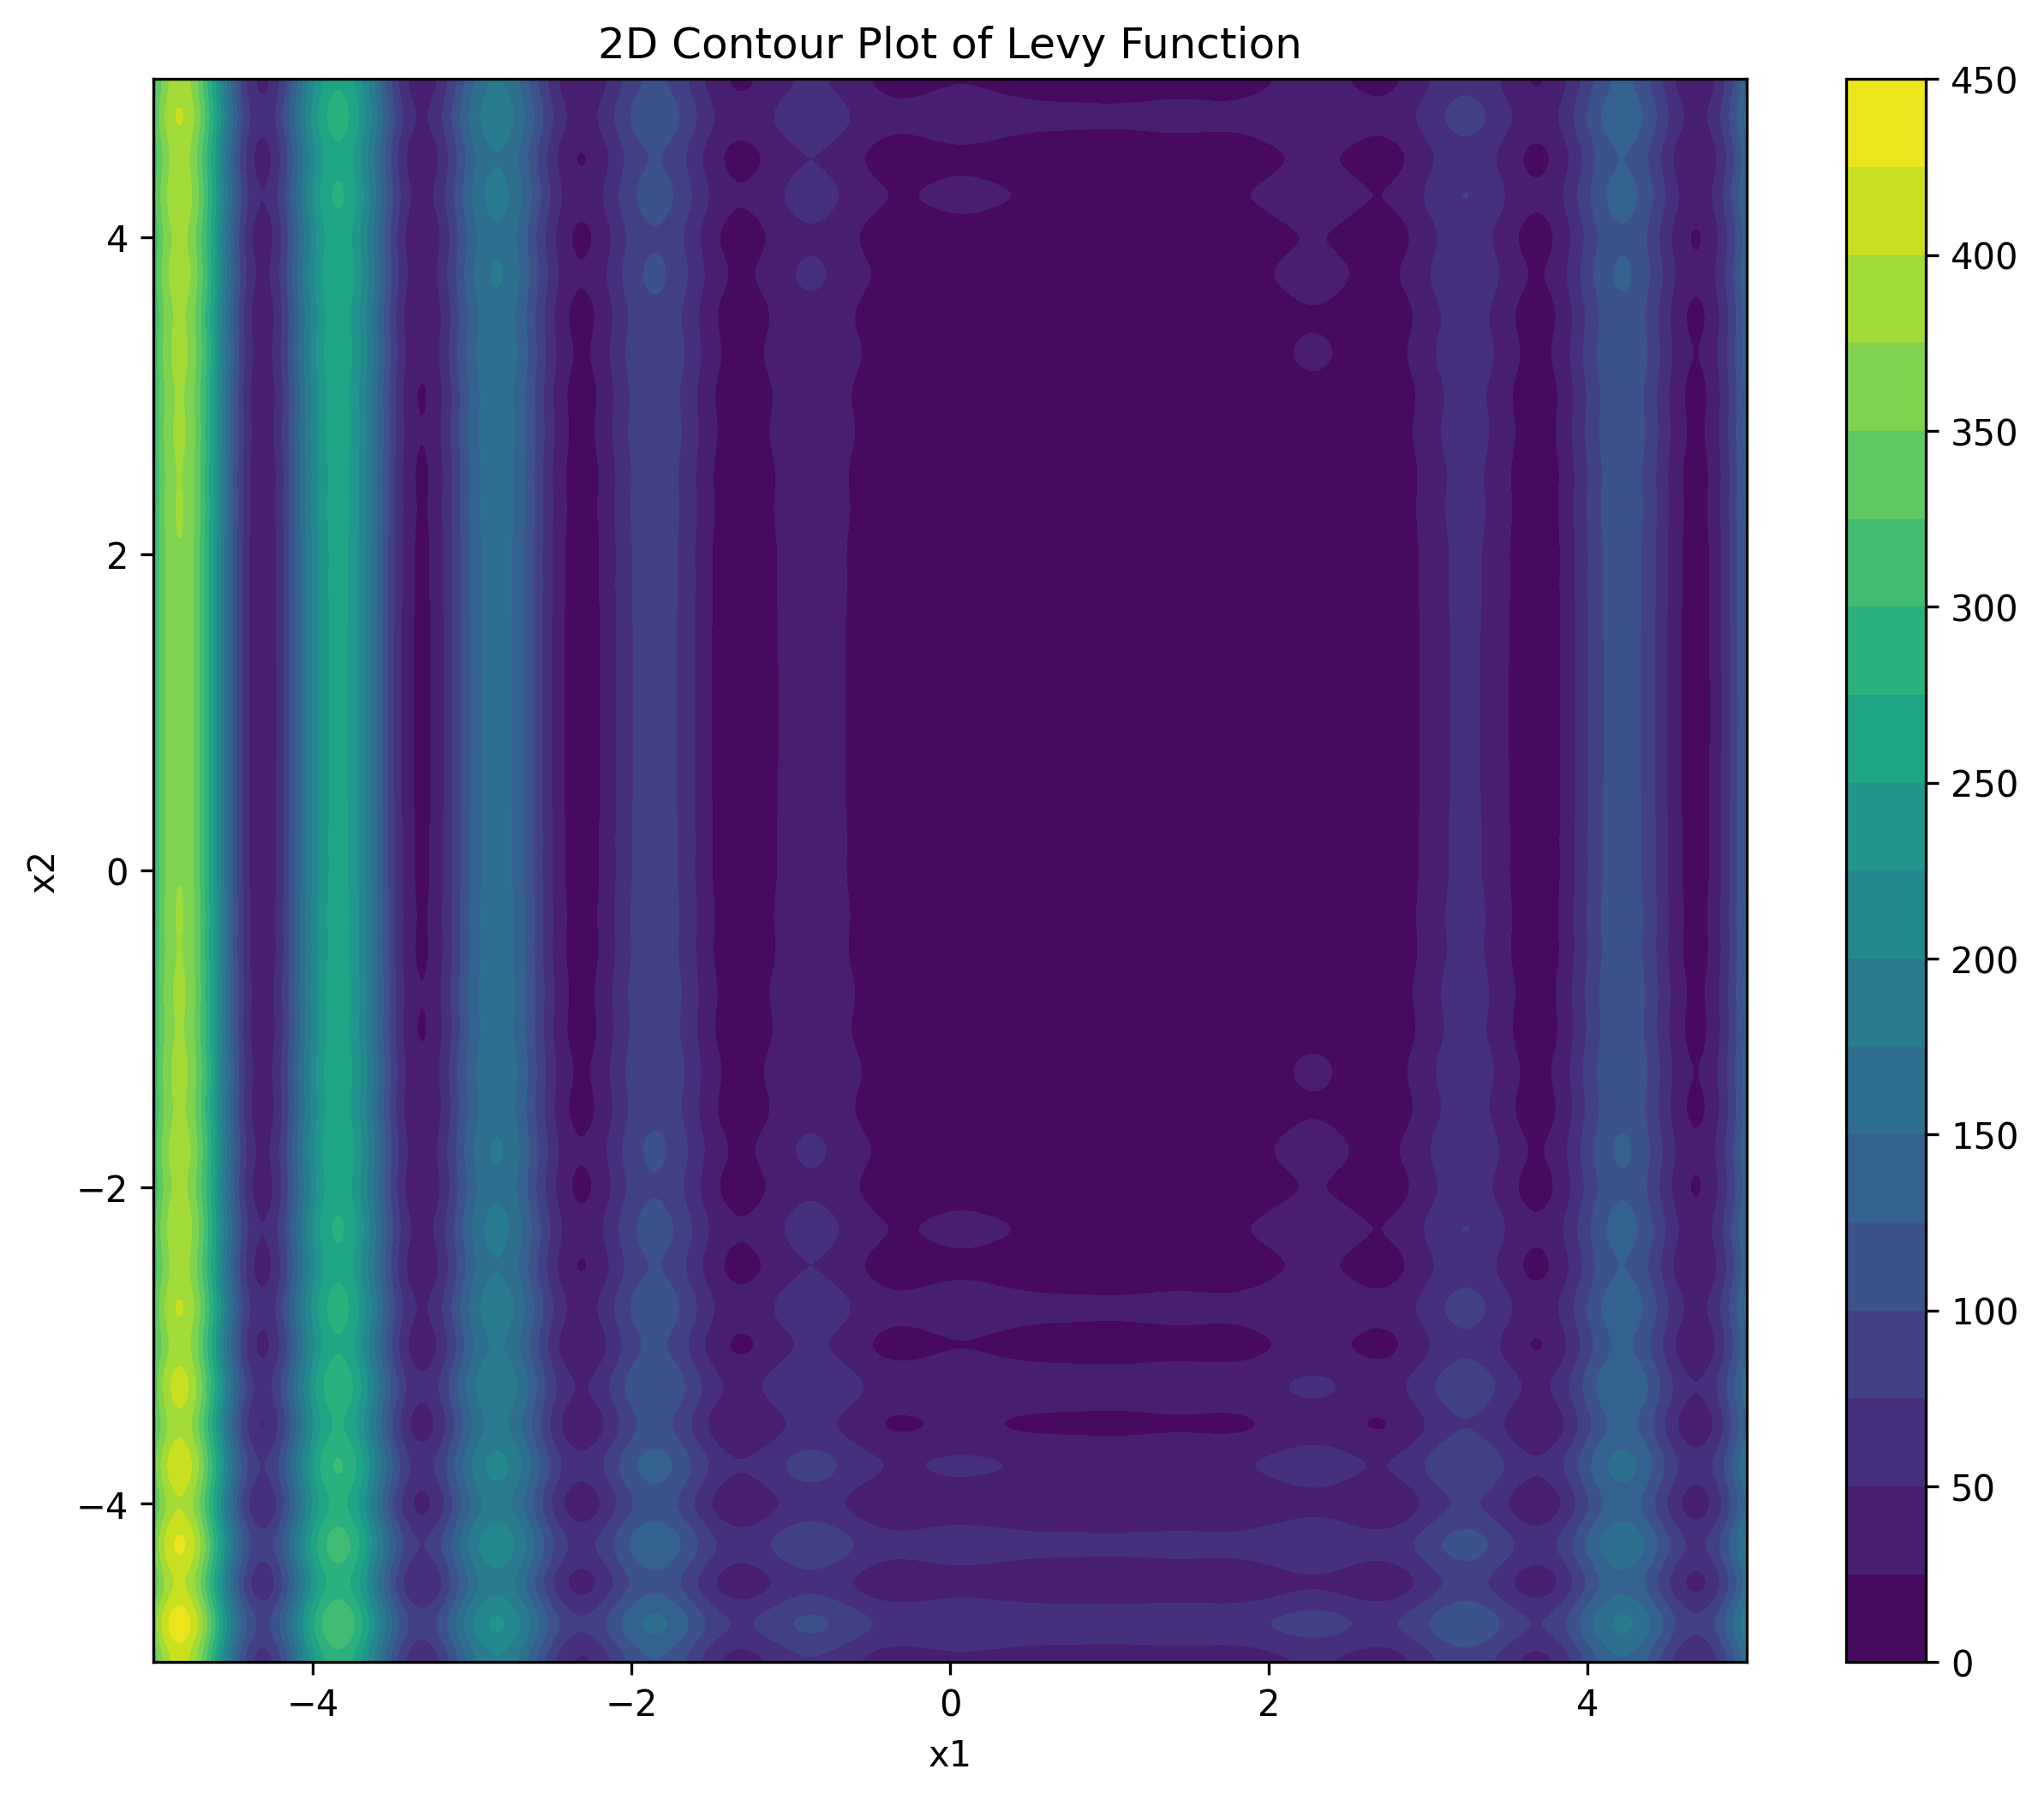
\includegraphics[width=\linewidth]{cec/levy_2d.png}
		\caption{Dimensi 2}
		\label{fig:levy-2d}
	\end{subfigure}
	\hfill
	\begin{subfigure}[b]{0.4\textwidth}
		\centering
		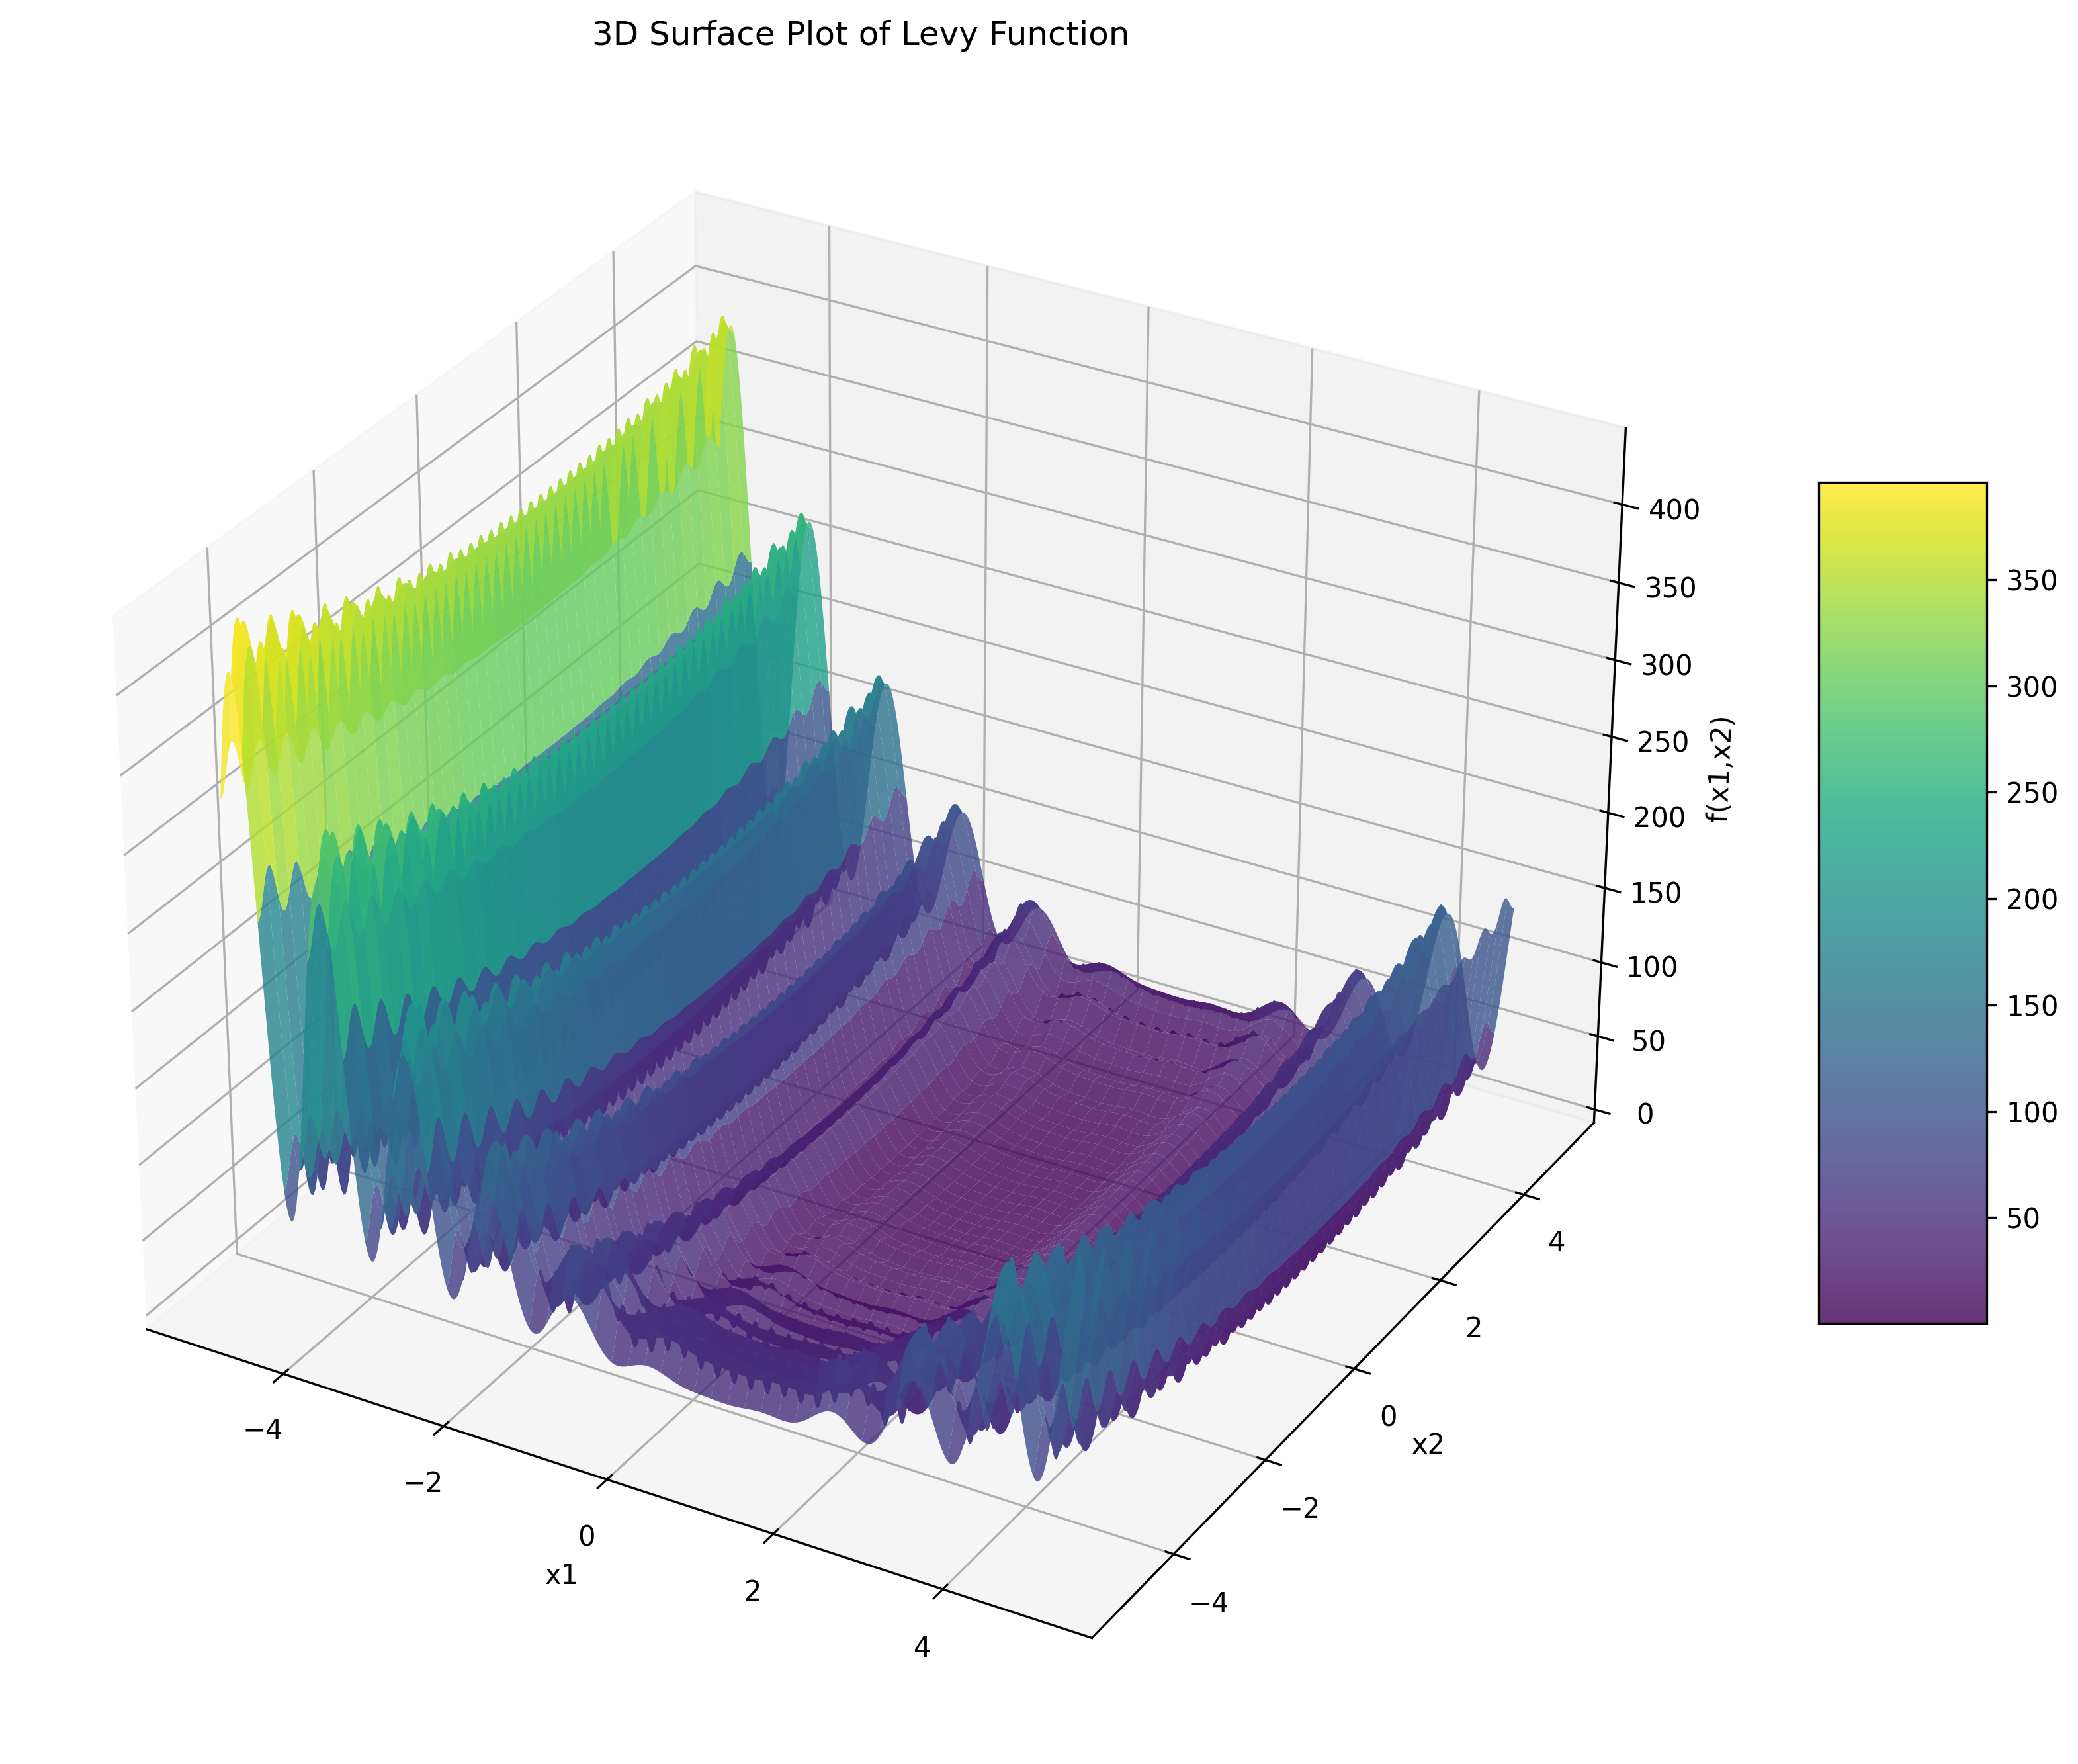
\includegraphics[width=\linewidth]{cec/levy_3d.png}
		\caption{Dimensi 3}
		\label{fig:levy-3d}
	\end{subfigure}
	\caption{Tampilan grafik fungsi Levy pada dimensi dua (\cref{fig:levy-2d}) dan tiga (\cref{fig:levy-3d})}
	\label{fig:levy}
\end{figure}
\begin{equation}
  f_{\text{Levy}}(\mathrm{x})=\sin^2\left(\pi w_1 \right)+\sum_{i=1}^{D-1}\left(w_i-1 \right)^2\left[1+10\sin^2\left( \pi w_i+1\right)\right]+\left(w_D-1 \right)\left[1+\sin^2\left( 2\pi w_D\right)  \right]+f_{\text{bias}}
\end{equation}
dimana $w_i=1+\frac{z_i-1}{4},\forall i=1,\ldots,D$

\subsubsection*{Rastrigin}
\noindent Properti:
\begin{packed_item}
  \item multimodal
  \item non-convex
  \item non-separable
  \item Local optima's number is huge
\end{packed_item}
\begin{figure}[H]
	\centering
	\begin{subfigure}[b]{0.4\textwidth}
		\centering
		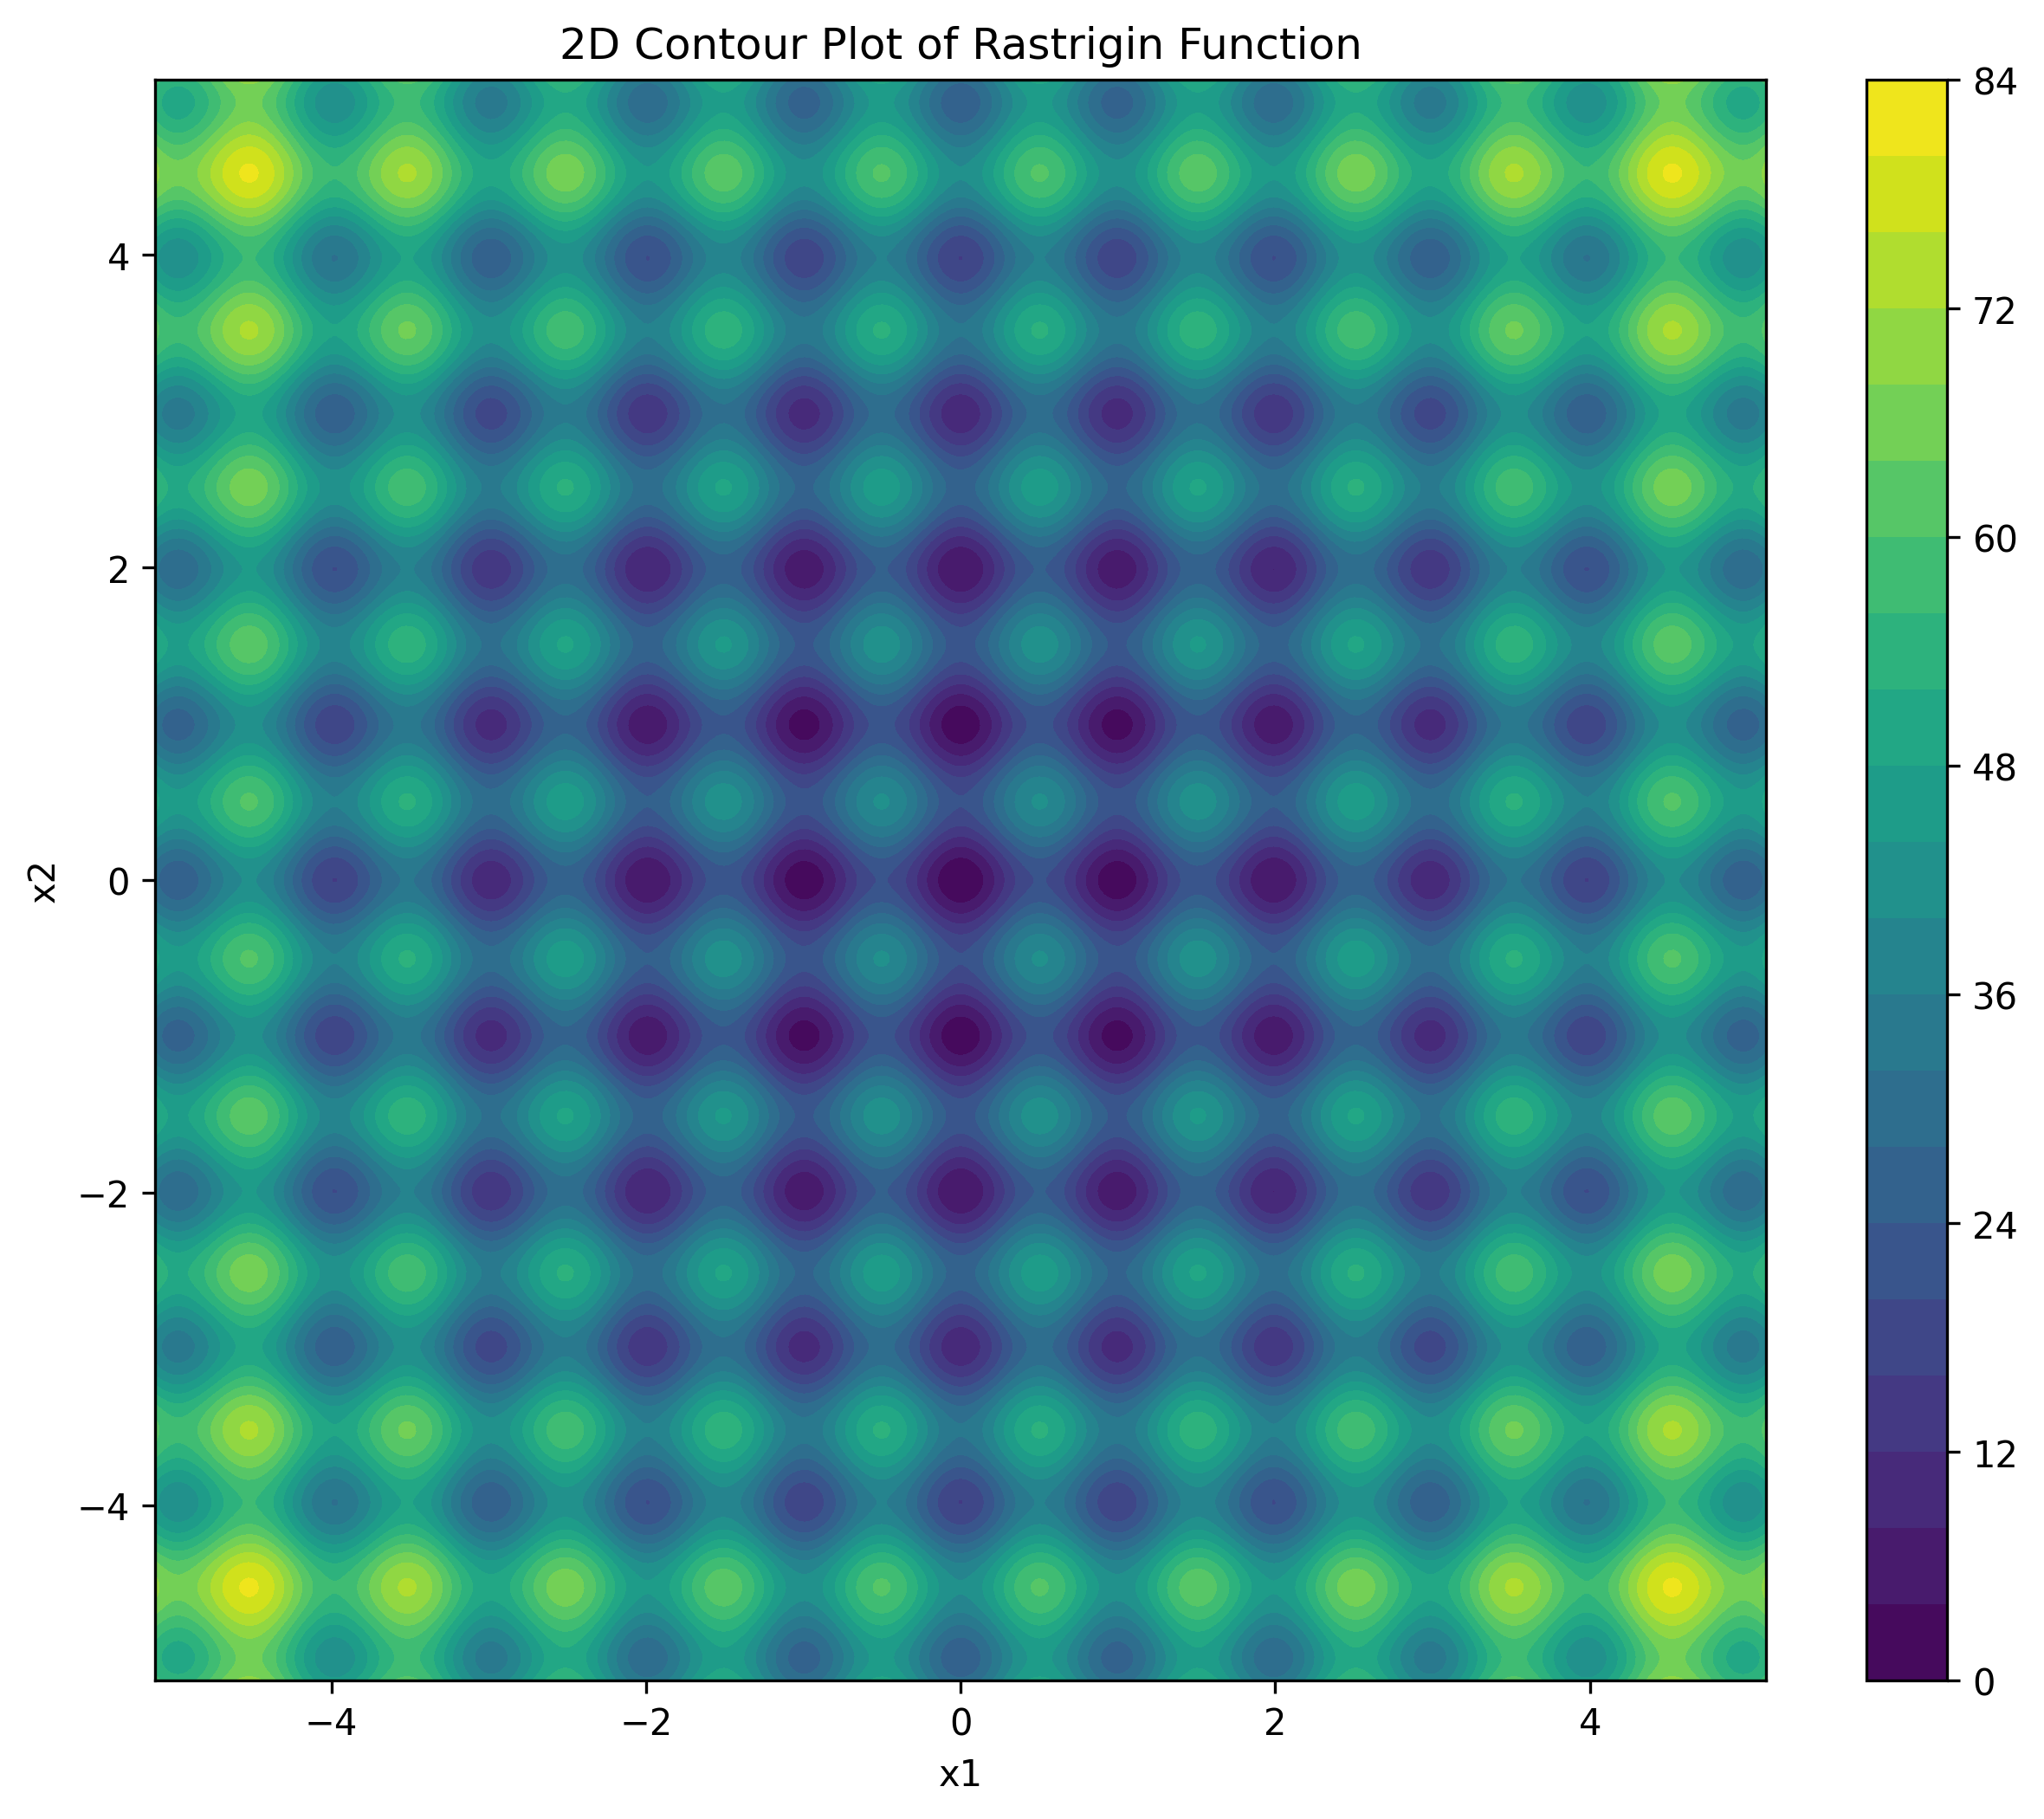
\includegraphics[width=\linewidth]{cec/rastrigin_2d.png}
		\caption{Dimensi 2}
		\label{fig:rastrigin-2d}
	\end{subfigure}
	\hfill
	\begin{subfigure}[b]{0.4\textwidth}
		\centering
		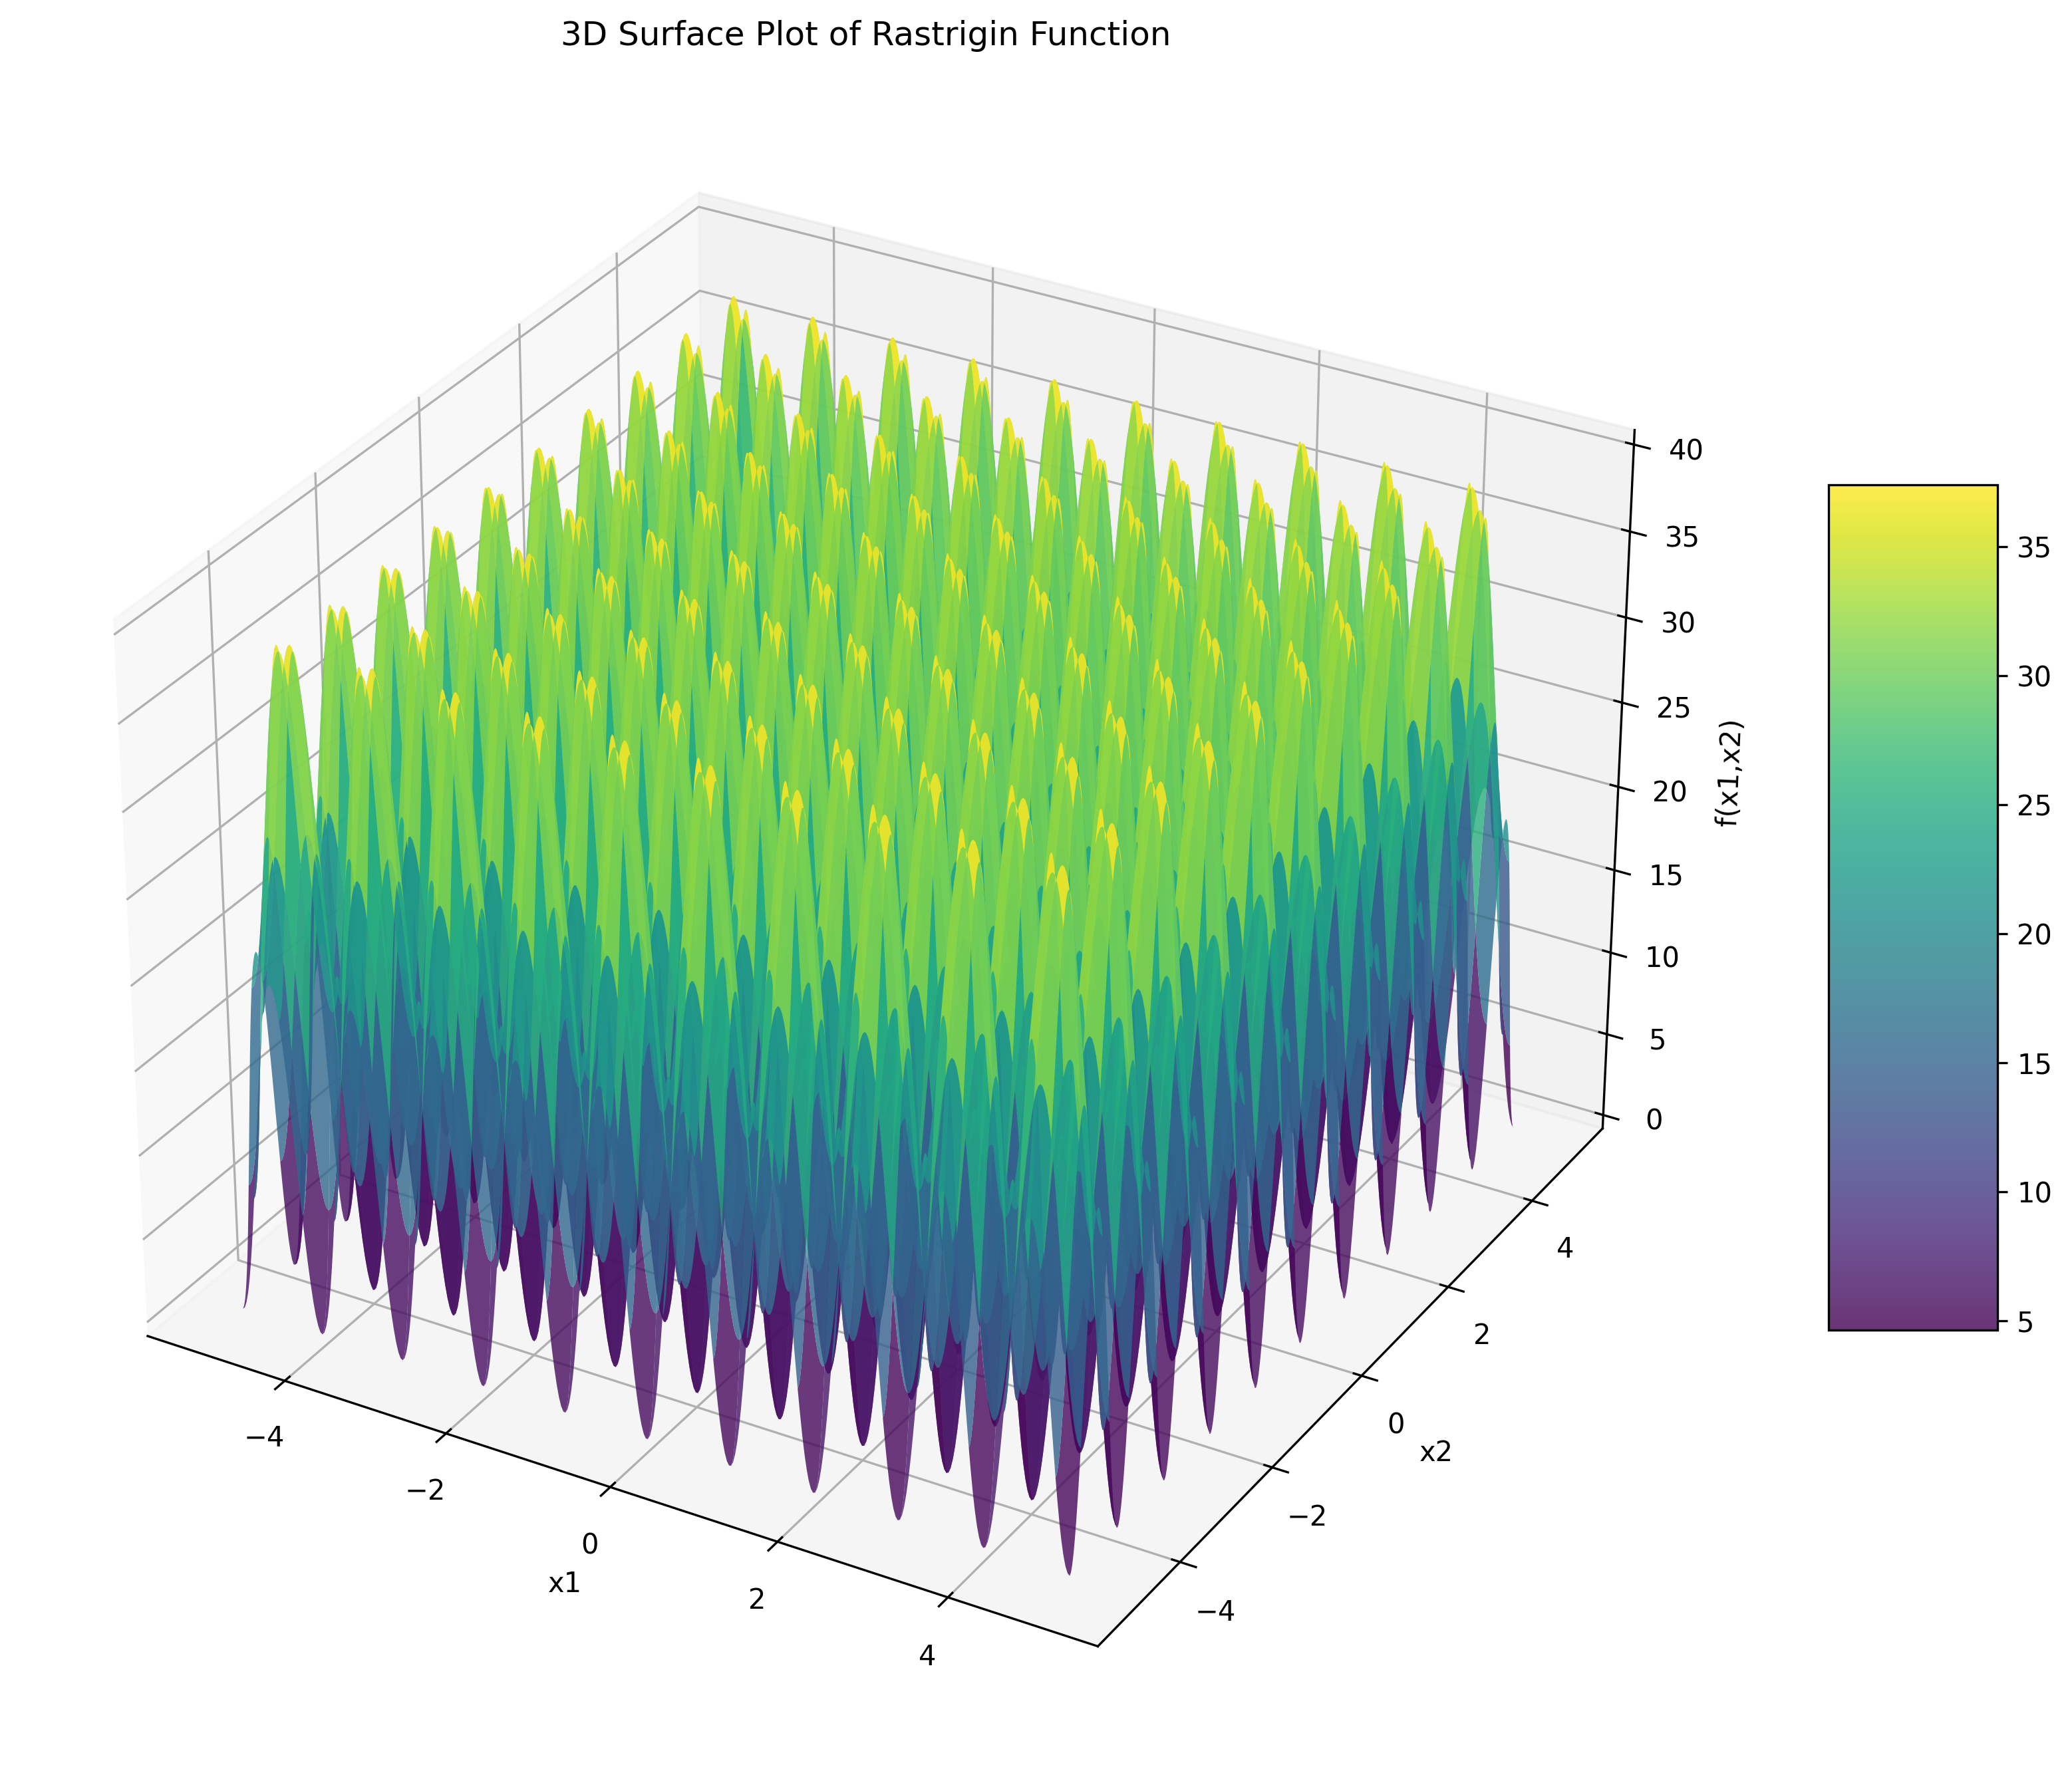
\includegraphics[width=\linewidth]{cec/rastrigin_3d.png}
		\caption{Dimensi 3}
		\label{fig:rastrigin-3d}
	\end{subfigure}
	\caption{Tampilan grafik fungsi Rastrigin pada dimensi dua (\cref{fig:rastrigin-2d}) dan tiga (\cref{fig:rastrigin-3d})}
	\label{fig:rastrigin}
\end{figure}
\begin{equation}
  f_{\text{Rastrigin}}(\mathrm{x})=\sum_{i=1}^{D}\left(z_i^2-10\cos\left(2\pi z_i \right)+10\right) +f_{\text{bias}}
\end{equation}

\subsubsection*{Rosenbrock}
\noindent Properti:
\begin{packed_item}
  \item multimodal
  \item non-convex
  \item non-separable
  \item Local optima's number is huge
\end{packed_item}
\begin{figure}[H]
	\centering
	\begin{subfigure}[b]{0.4\textwidth}
		\centering
		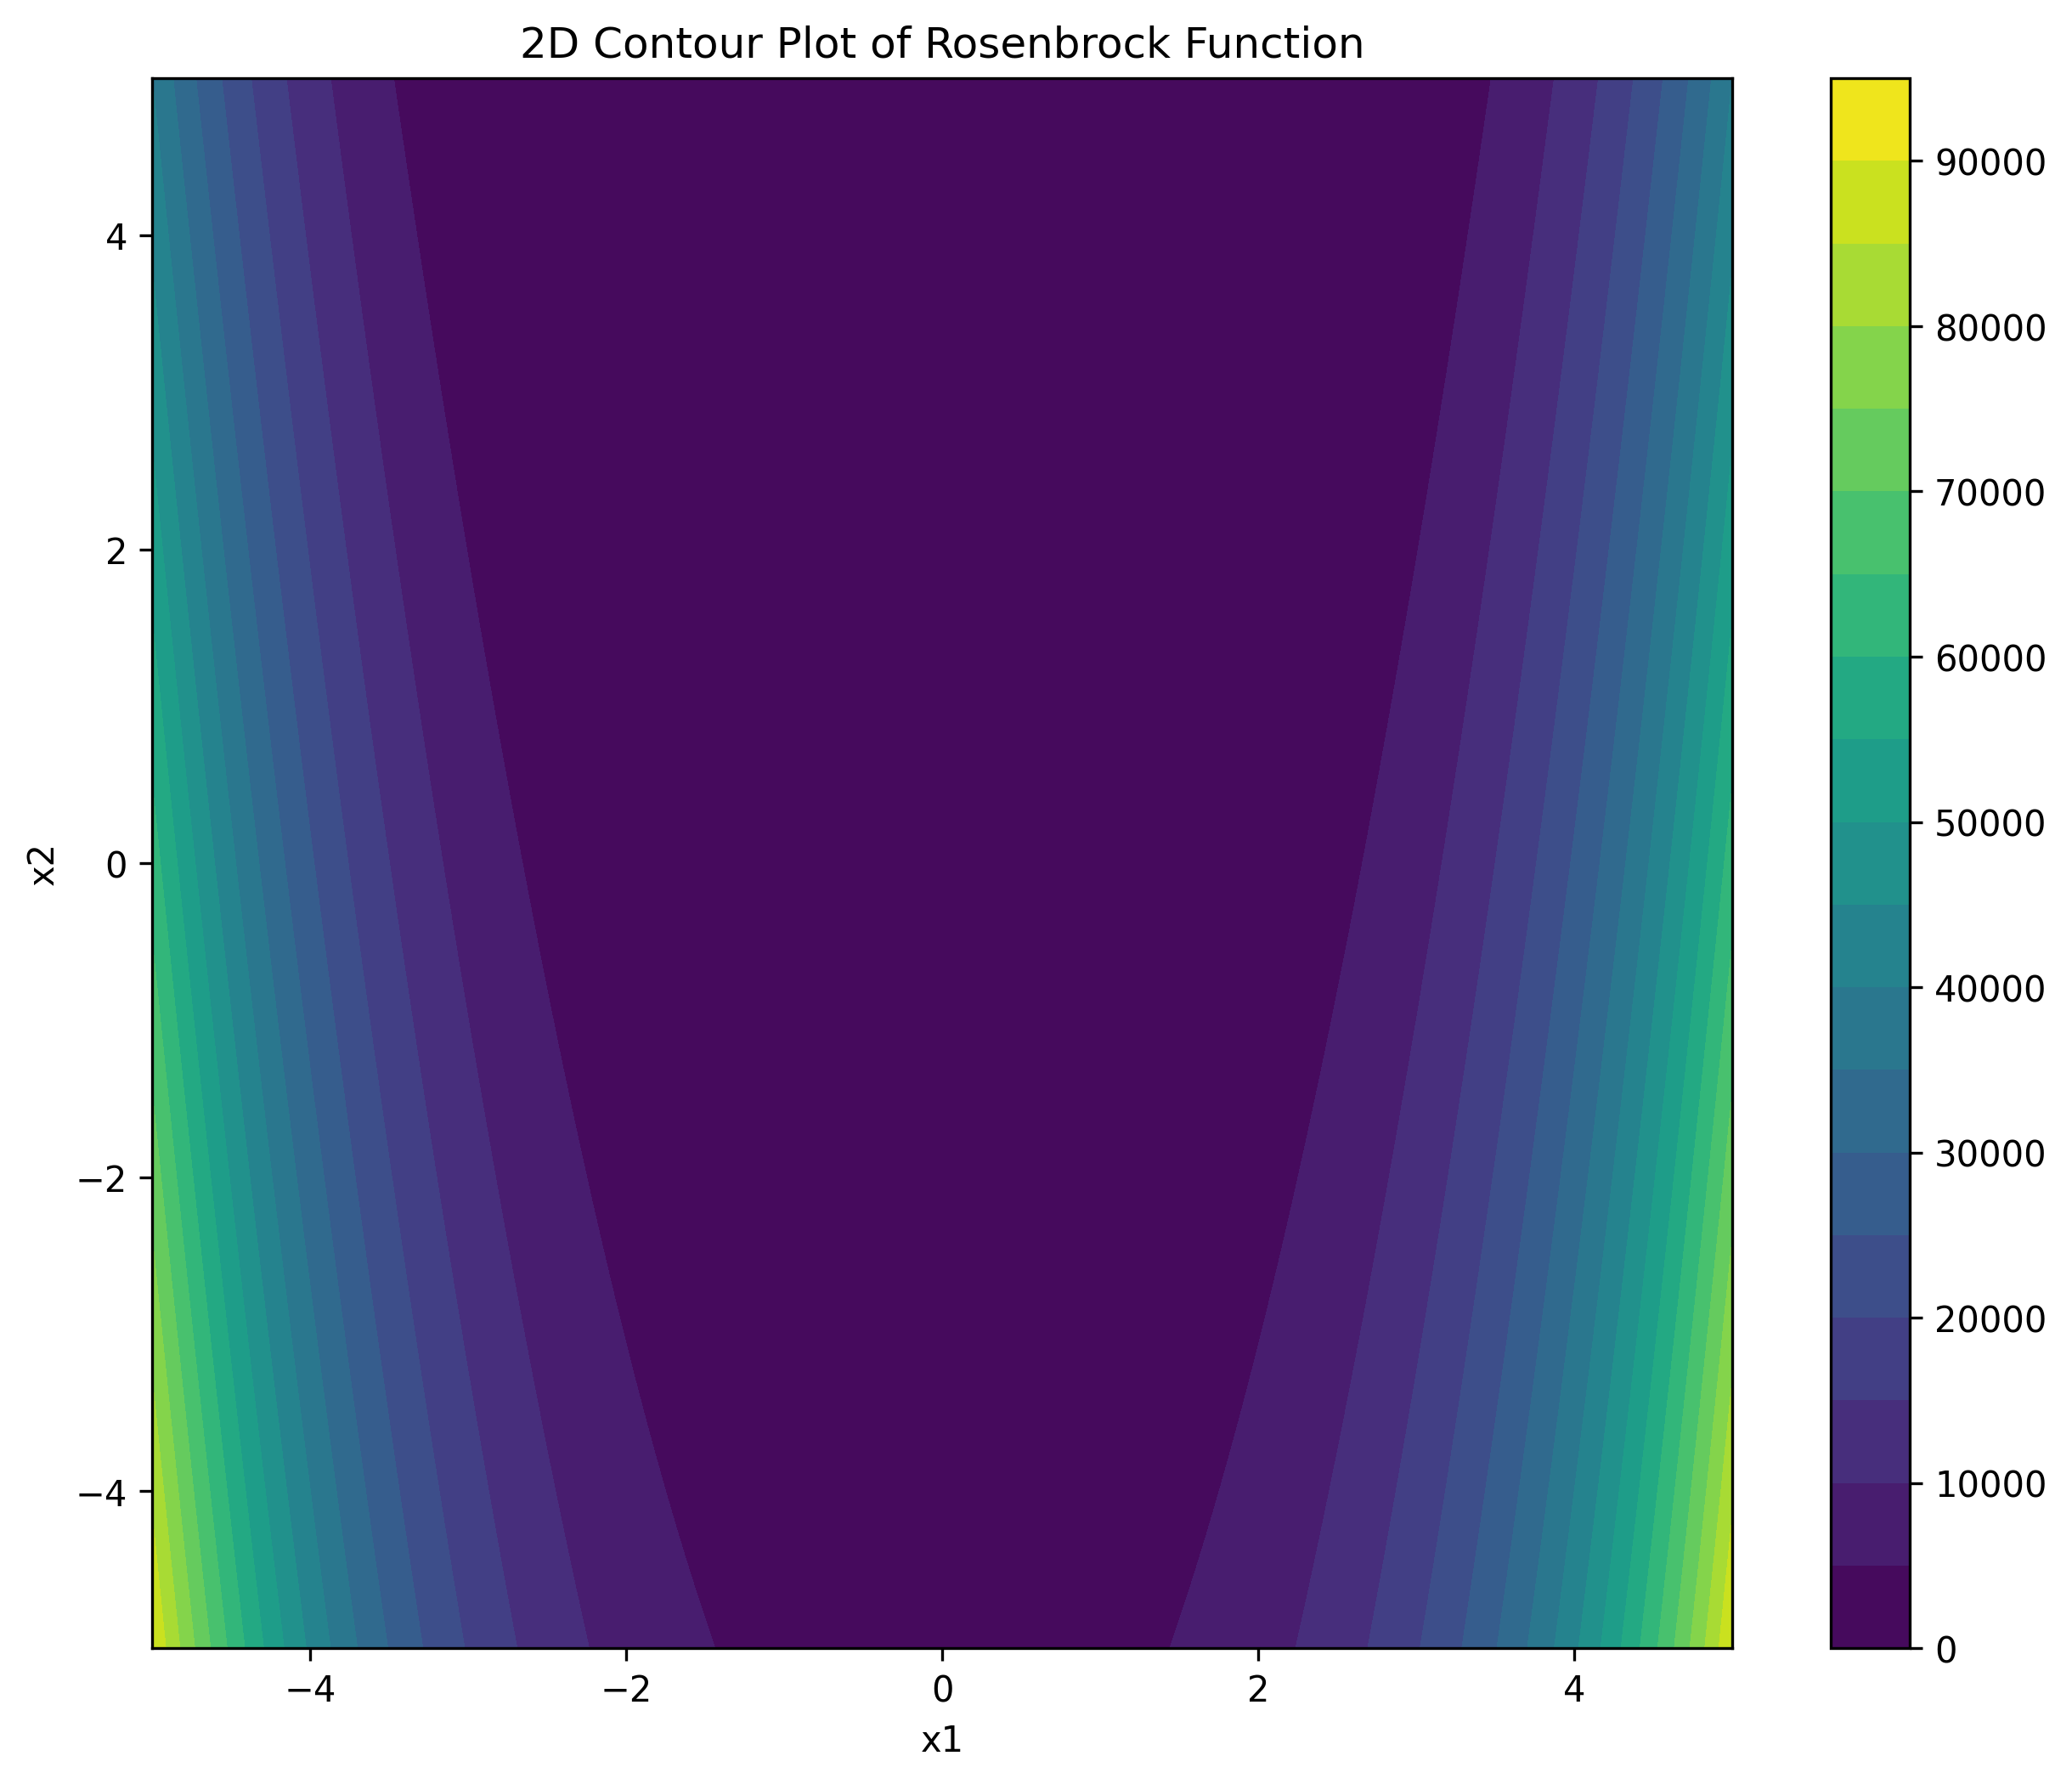
\includegraphics[width=\linewidth]{cec/rosenbrock_2d.png}
		\caption{Dimensi 2}
		\label{fig:rosenbrock-2d}
	\end{subfigure}
	\hfill
	\begin{subfigure}[b]{0.4\textwidth}
		\centering
		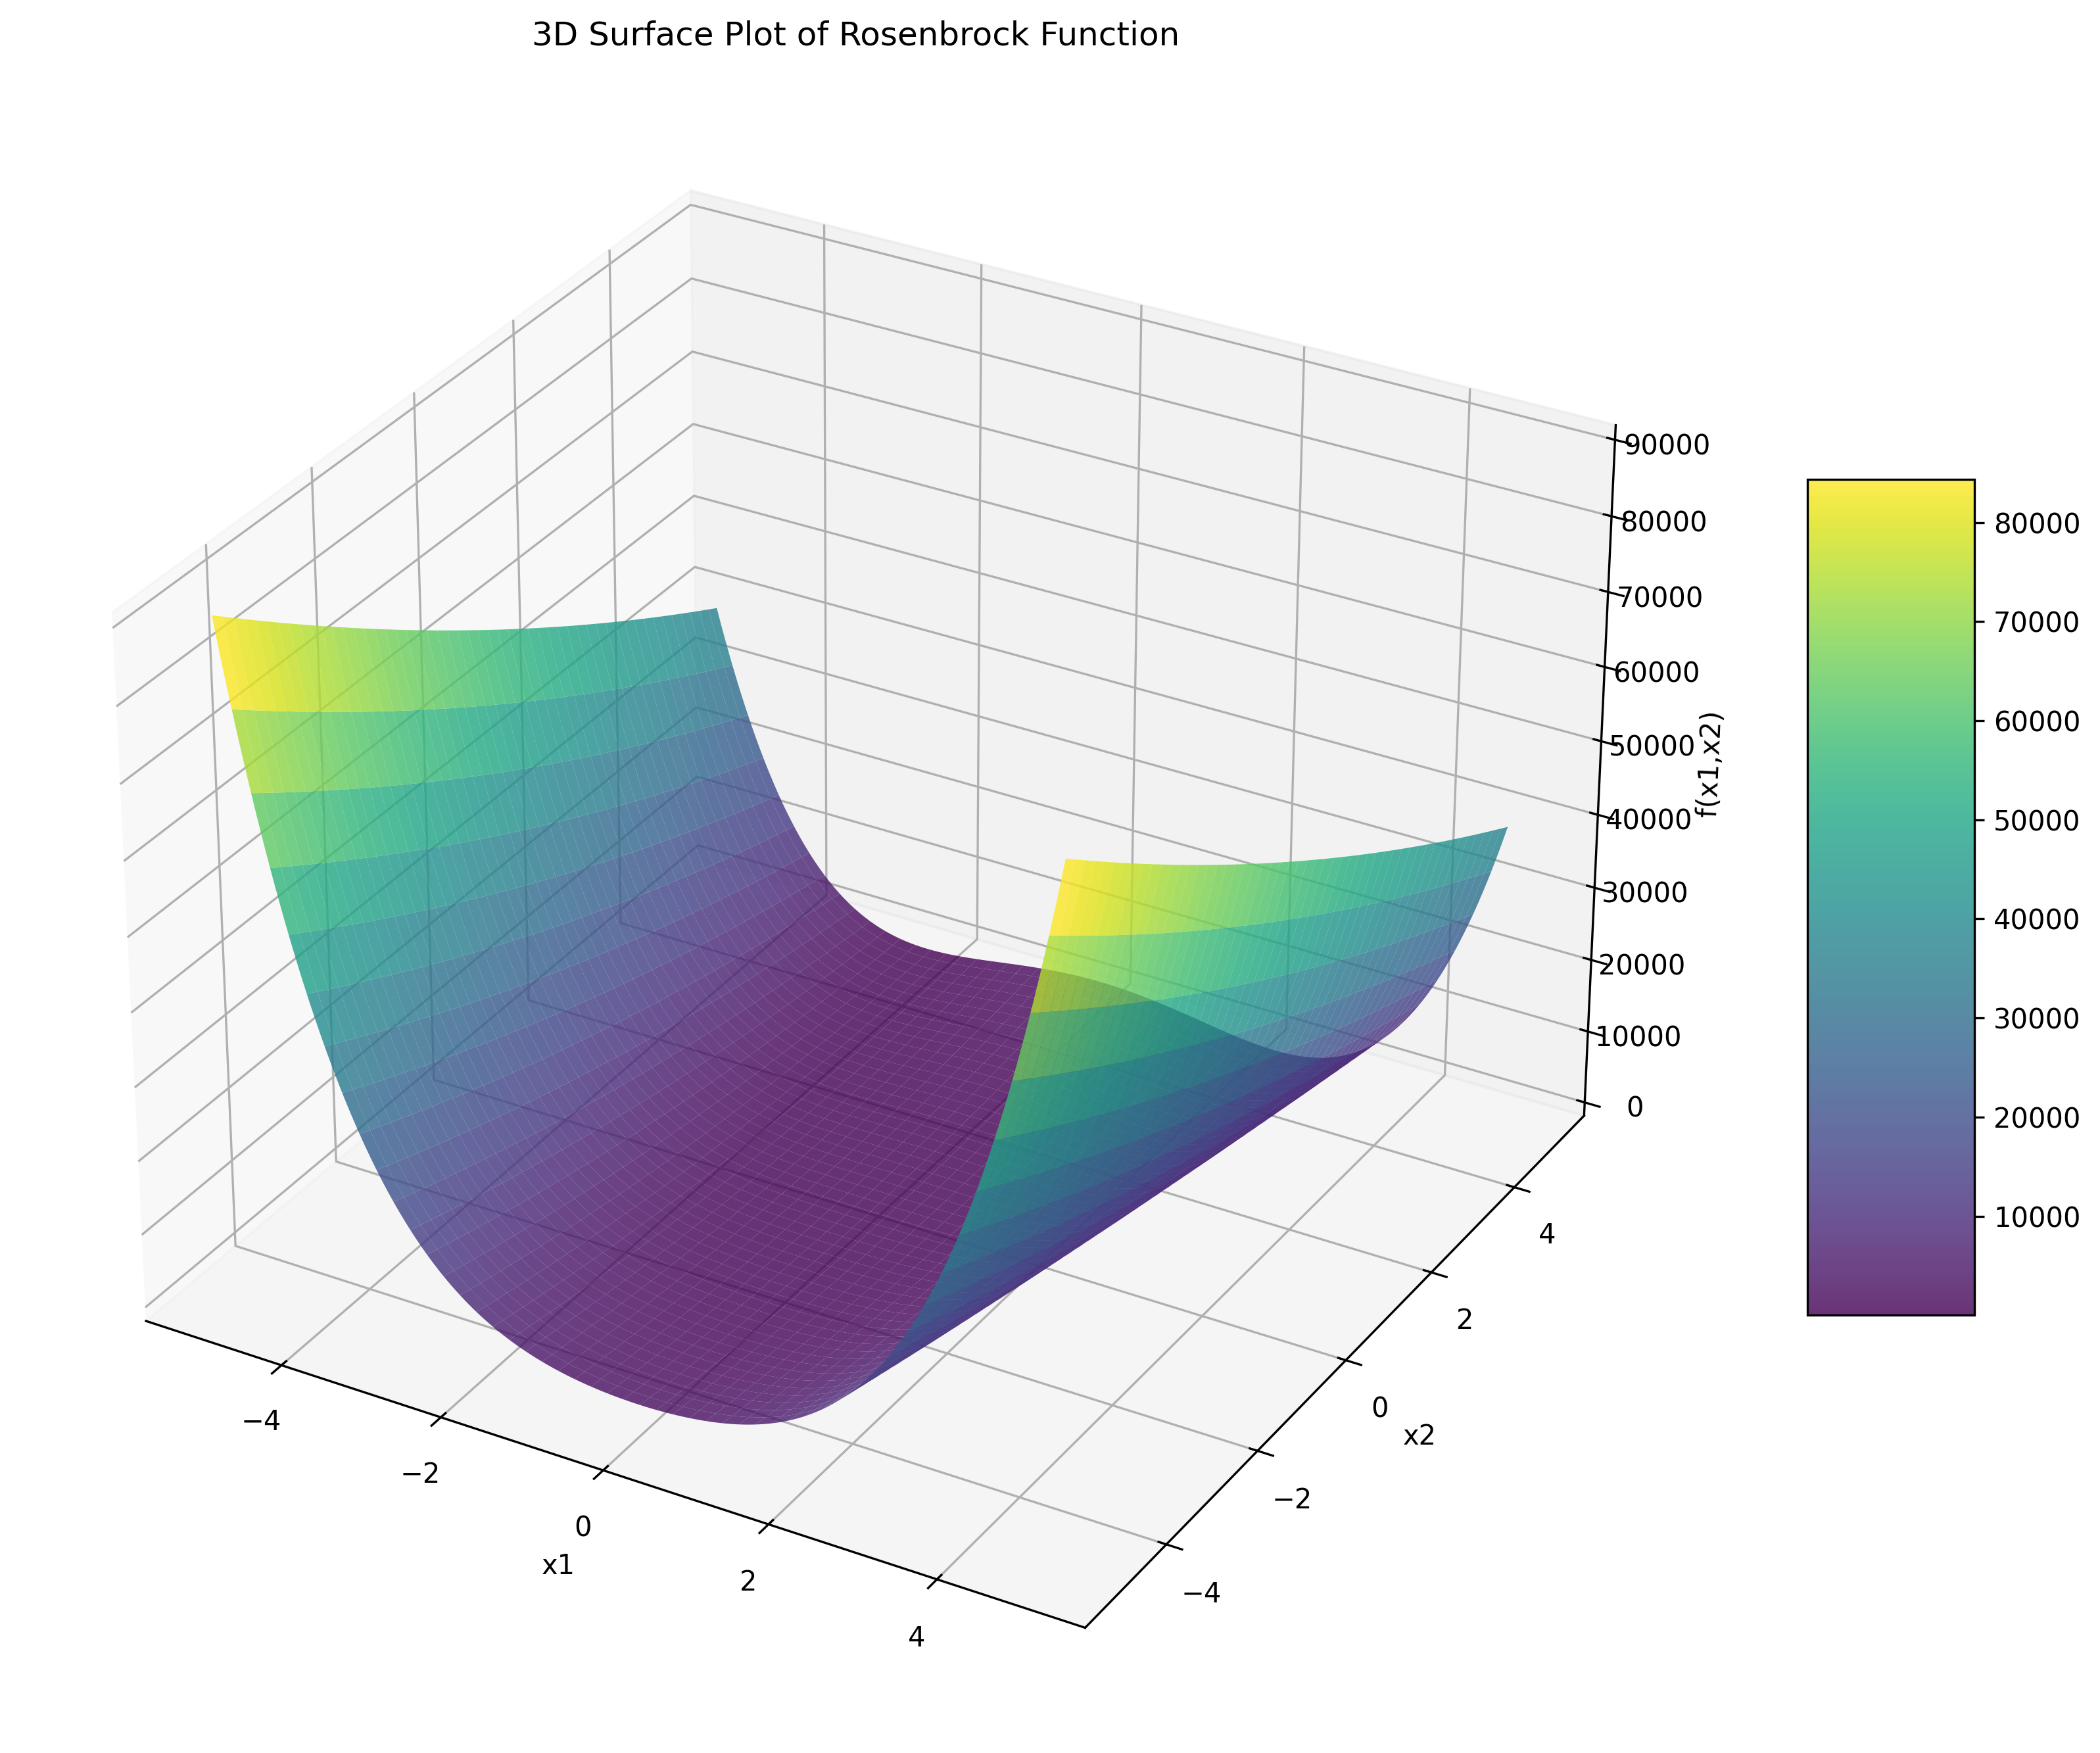
\includegraphics[width=\linewidth]{cec/rosenbrock_3d.png}
		\caption{Dimensi 3}
		\label{fig:rosenbrock-3d}
	\end{subfigure}
	\caption{Tampilan grafik fungsi Rosenbrock pada dimensi dua (\cref{fig:rosenbrock-2d}) dan tiga (\cref{fig:rosenbrock-3d})}
	\label{fig:rosenbrock}
\end{figure}
\begin{equation}
  f_{\text{Rosenbrock}}(\mathrm{x})=\sum_{i=1}^{D-1}\left(100\left(z_i^2-z_{i+1} \right)^2+\left( z_i-1\right)^2 \right) +f_{\text{bias}}
\end{equation}

\subsubsection*{Schwefel 1.2 Problem}
\noindent Properti:
\begin{packed_item}
  \item unimodal
  \item convex
  \item non-separable
  \item scalable
\end{packed_item}
\begin{figure}[H]
	\centering
	\begin{subfigure}[b]{0.4\textwidth}
		\centering
		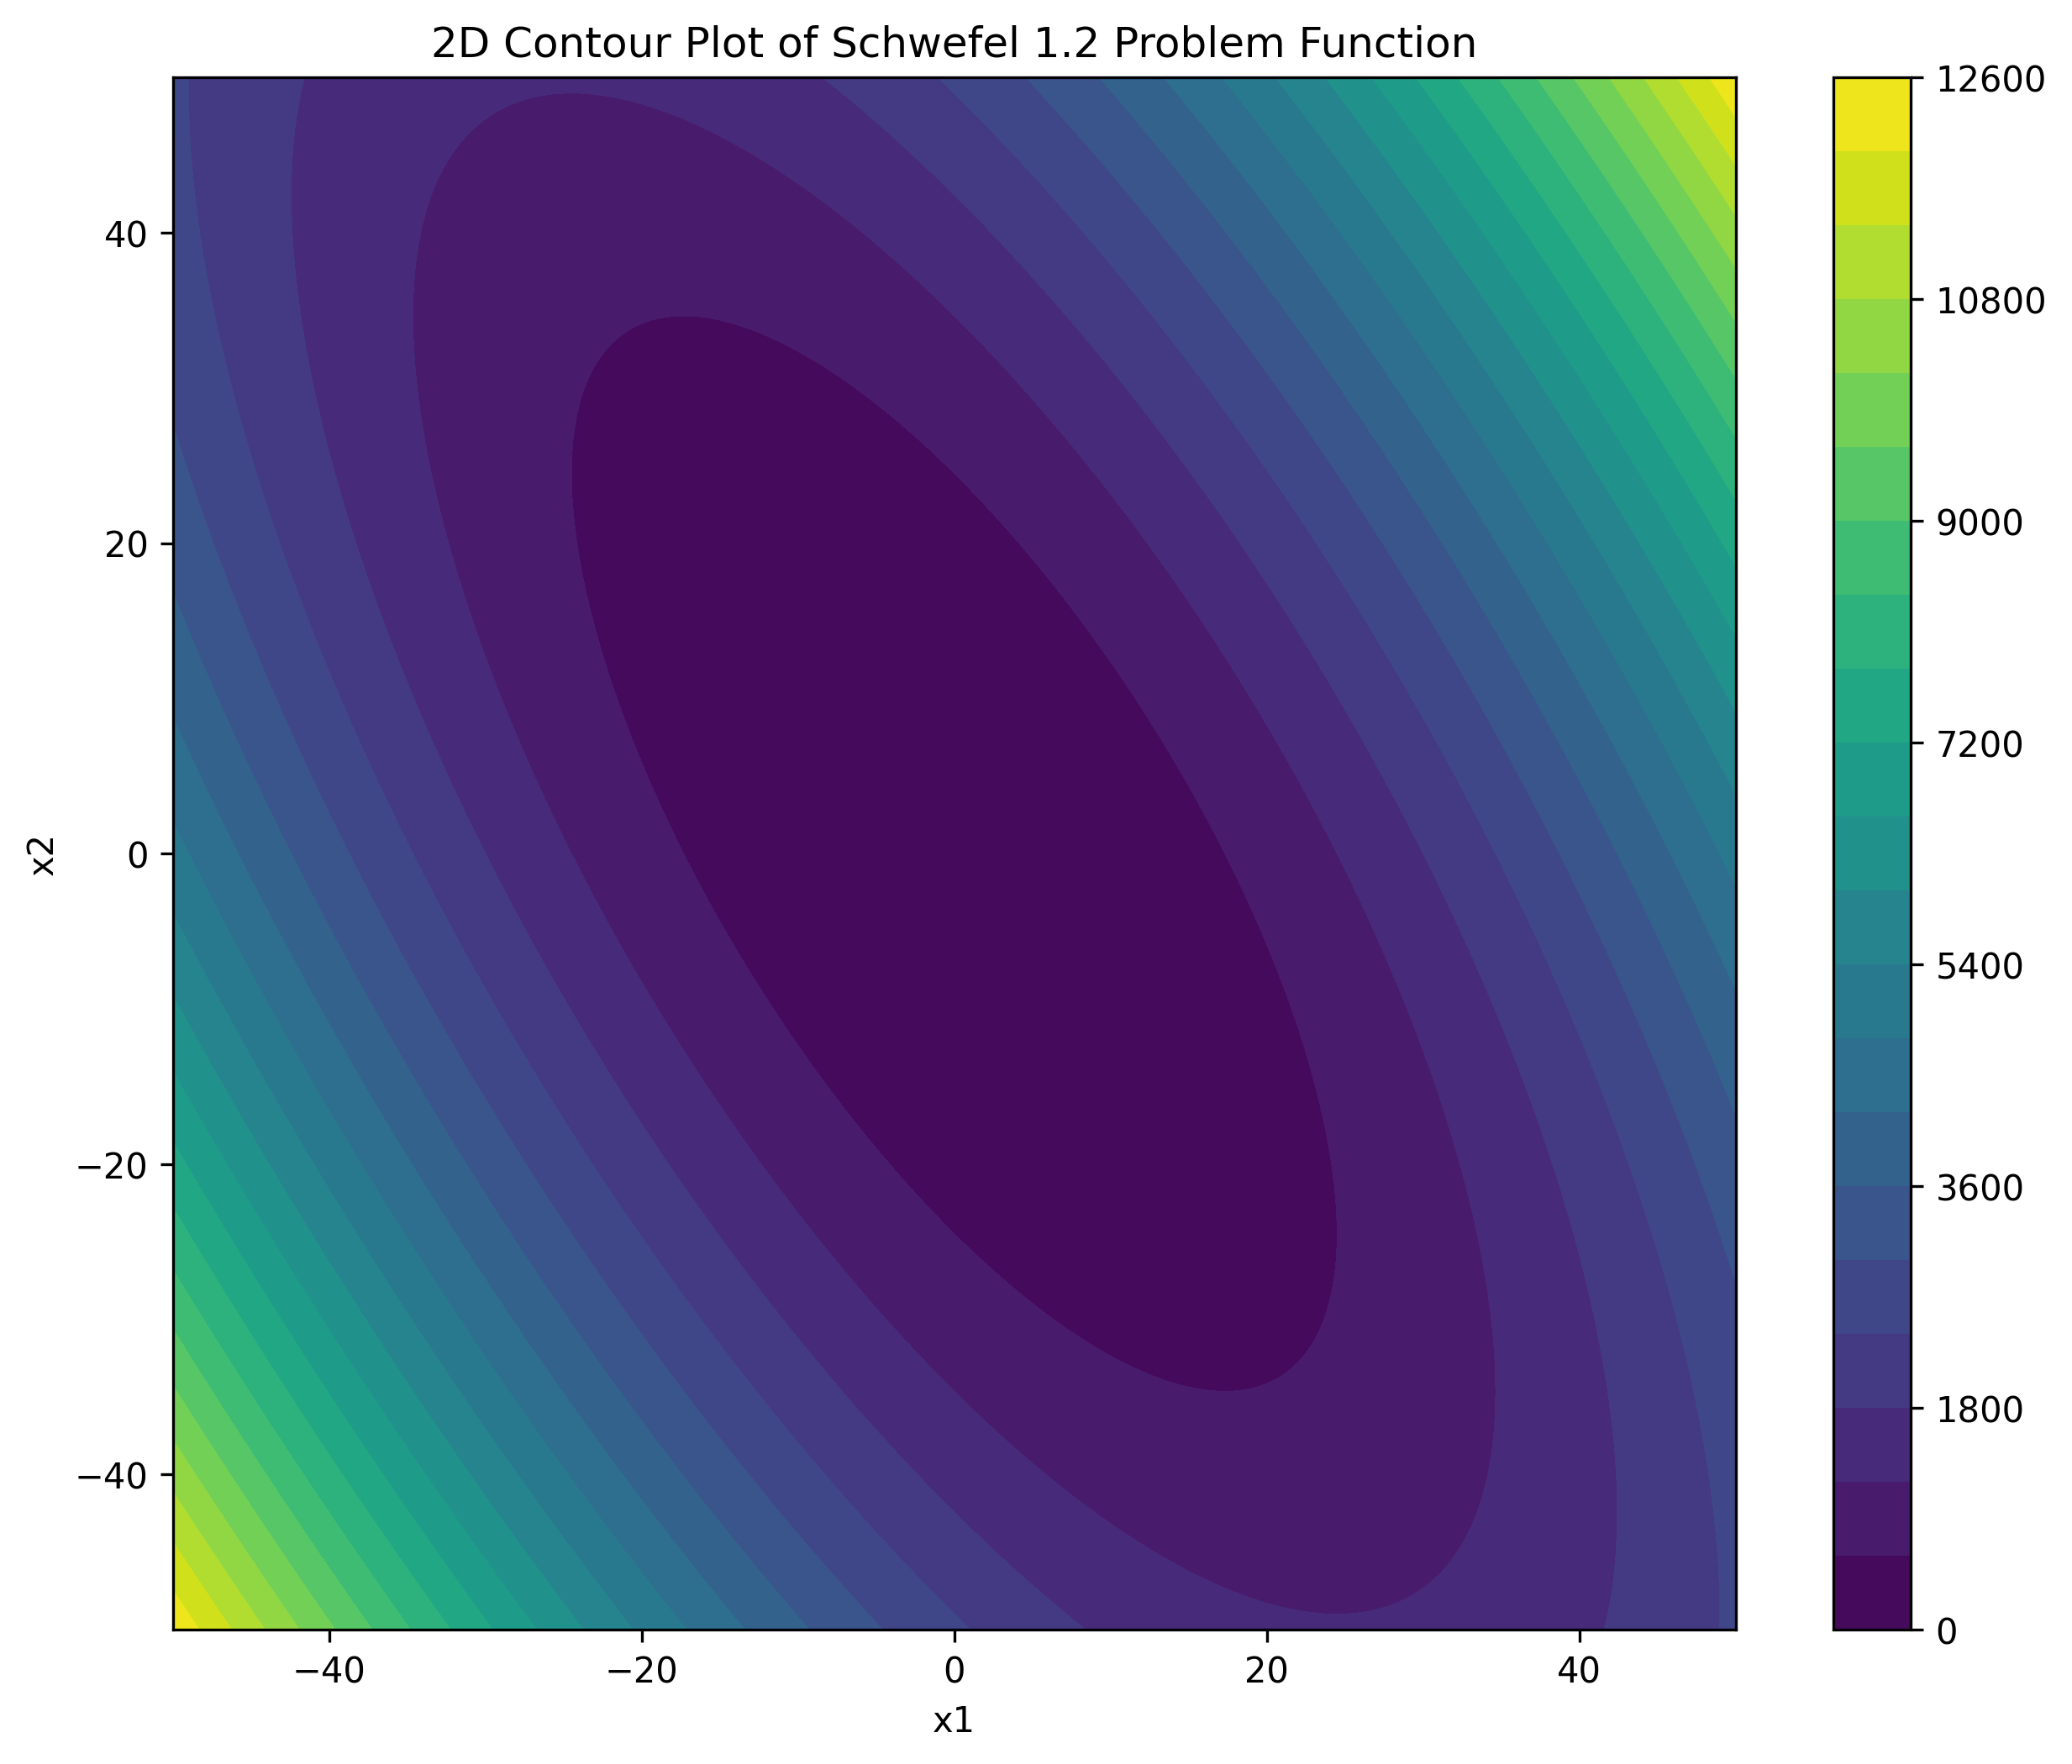
\includegraphics[width=\linewidth]{cec/schwefel1_2_2d.png}
		\caption{Dimensi 2}
		\label{fig:schwefel1_2-2d}
	\end{subfigure}
	\hfill
	\begin{subfigure}[b]{0.4\textwidth}
		\centering
		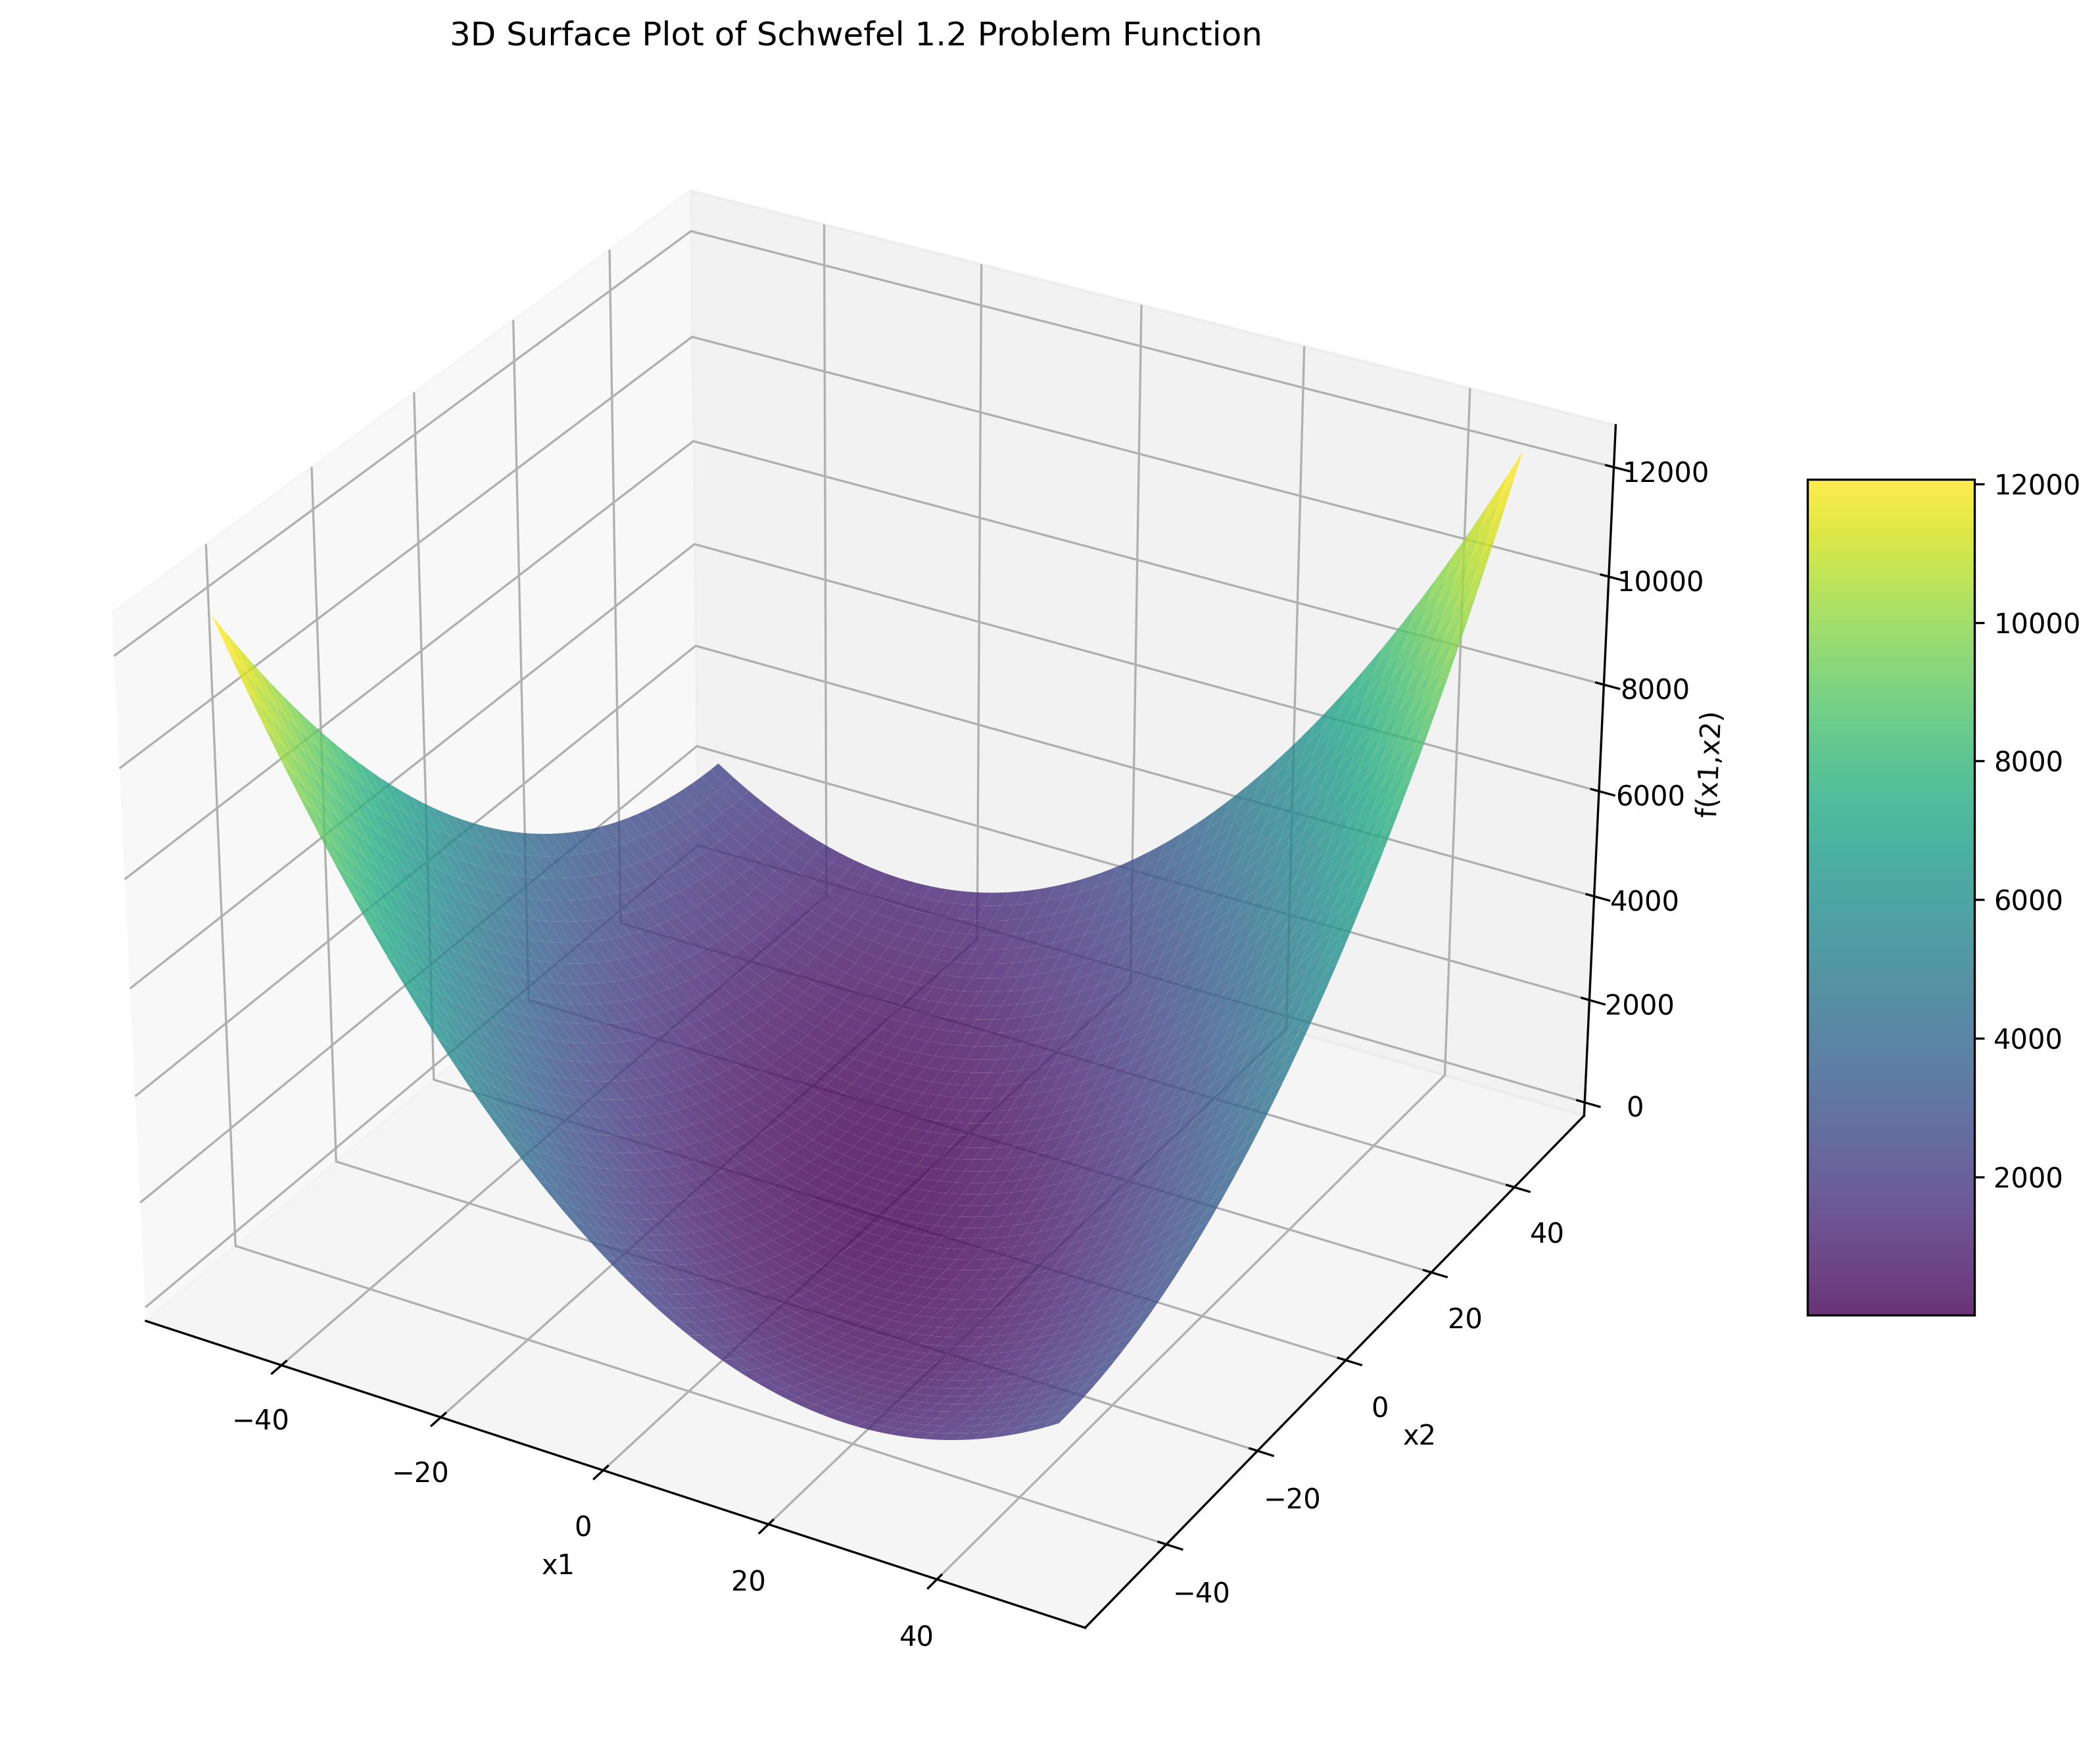
\includegraphics[width=\linewidth]{cec/schwefel1_2_3d.png}
		\caption{Dimensi 3}
		\label{fig:schwefel1_2-3d}
	\end{subfigure}
	\caption{Tampilan grafik fungsi Schwefel 1.2 Problem pada dimensi dua (\cref{fig:schwefel1_2-2d}) dan tiga (\cref{fig:schwefel1_2-3d})}
	\label{fig:schwefel1_2}
\end{figure}
\begin{equation}
  f_{\text{Schwefel 1.2}}(\mathrm{x})=\sum_{i=1}^{D}\left(\sum_{j=1}^{i}z_j \right)^2 +f_{\text{bias}}
\end{equation}

\subsubsection*{Schwefel 2.13 Problem}
\noindent Properti:
\begin{packed_item}
  \item multimodal
  \item non-convex
  \item non-separable
  \item scalable
\end{packed_item}
\begin{figure}[H]
	\centering
	\begin{subfigure}[b]{0.4\textwidth}
		\centering
		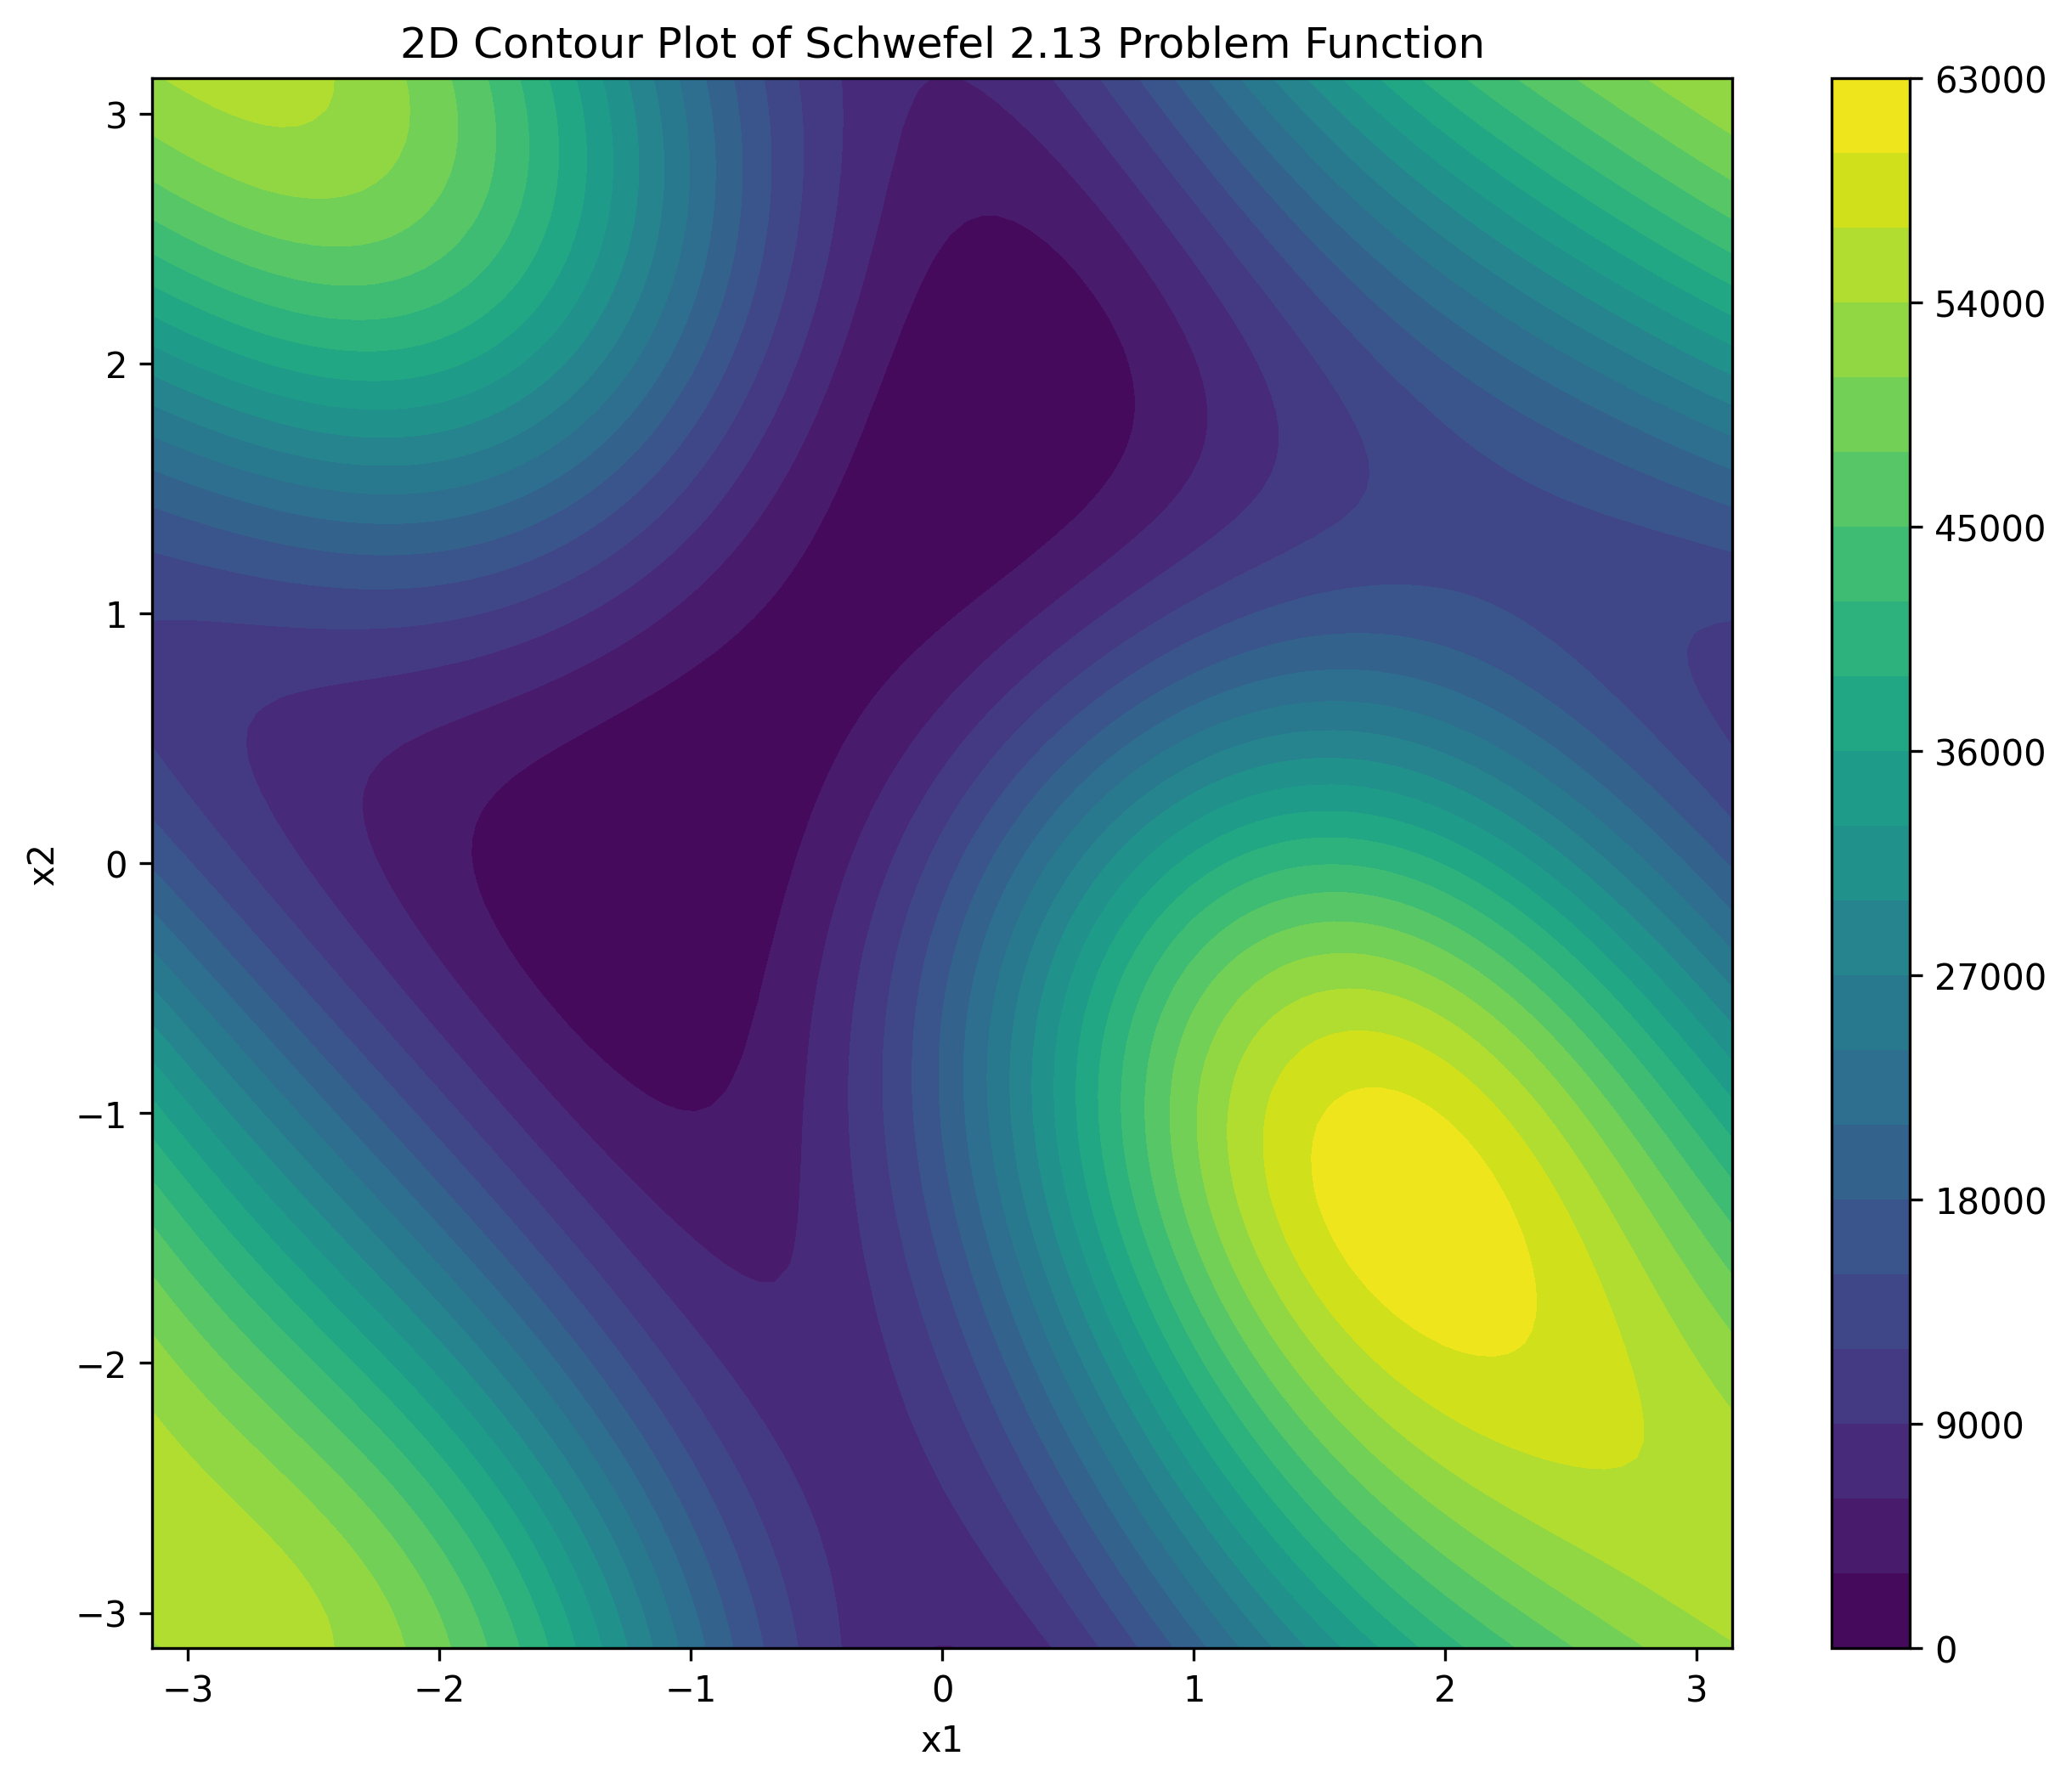
\includegraphics[width=\linewidth]{cec/schwefel2_13_2d.png}
		\caption{Dimensi 2}
		\label{fig:schwefel2_13-2d}
	\end{subfigure}
	\hfill
	\begin{subfigure}[b]{0.4\textwidth}
		\centering
		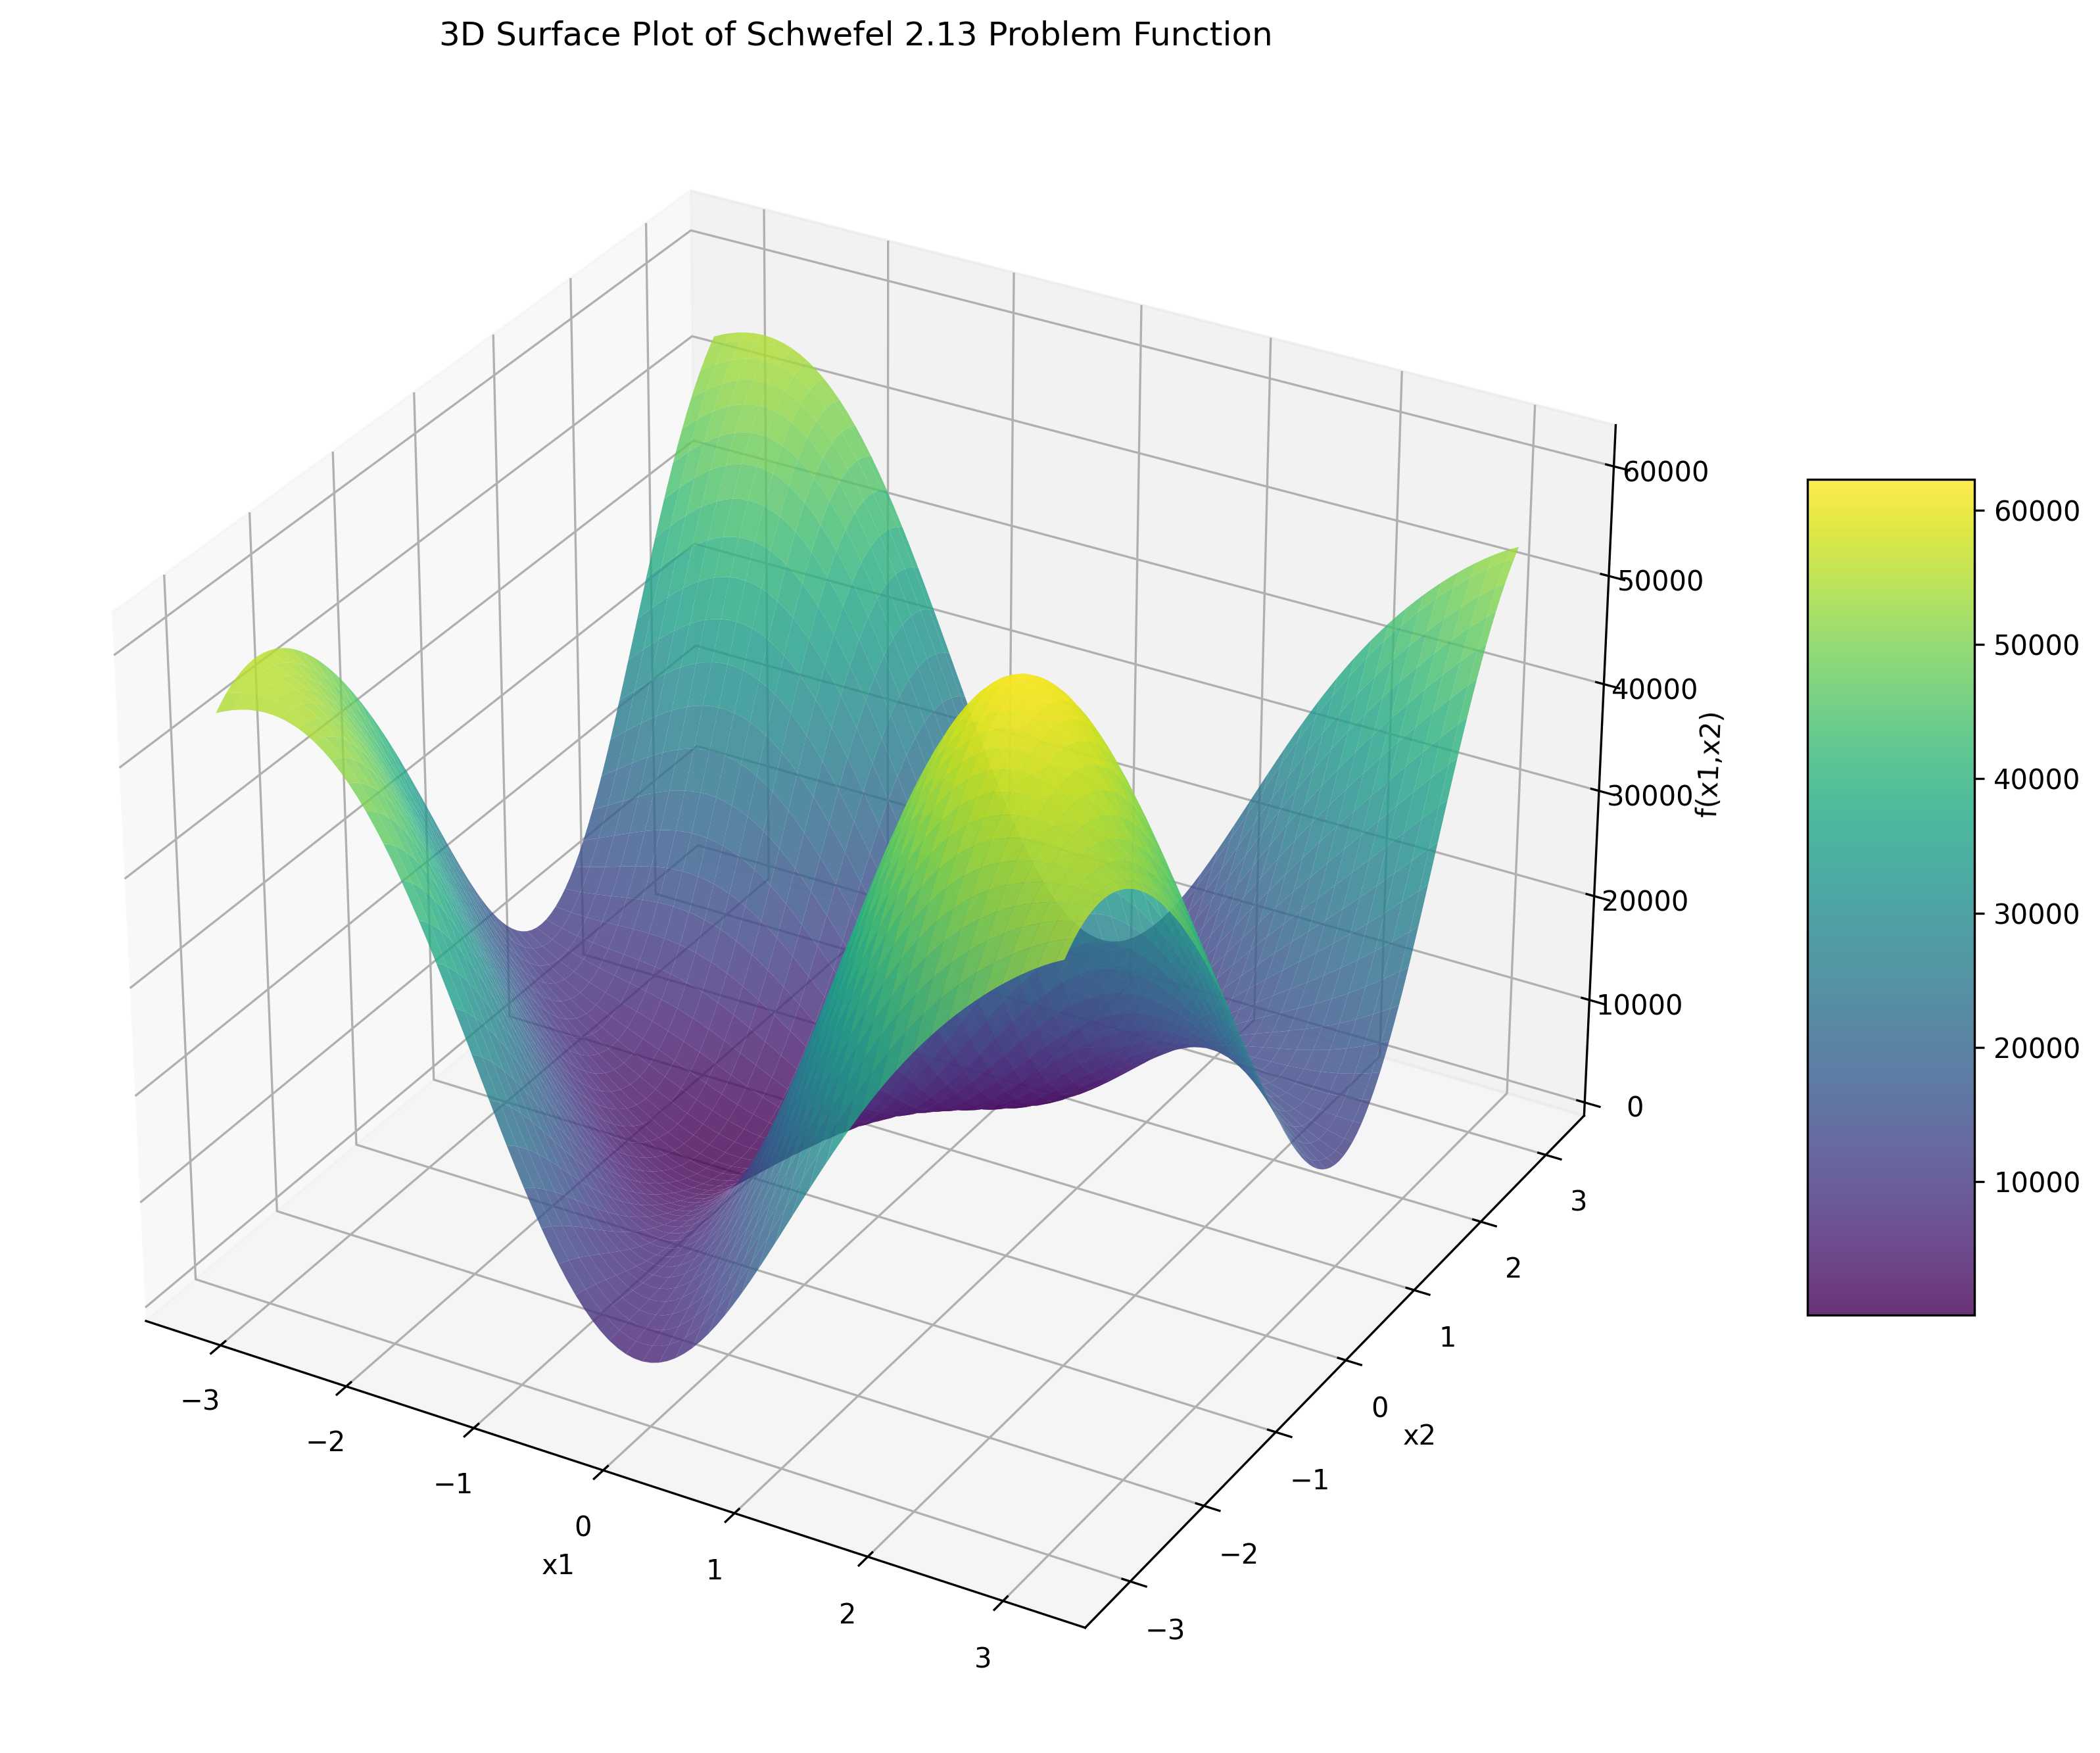
\includegraphics[width=\linewidth]{cec/schwefel2_13_3d.png}
		\caption{Dimensi 3}
		\label{fig:schwefel2_13-3d}
	\end{subfigure}
	\caption{Tampilan grafik fungsi Schwefel 2.13 Problem pada dimensi dua (\cref{fig:schwefel2_13-2d}) dan tiga (\cref{fig:schwefel2_13-3d})}
	\label{fig:schwefel2_13}
\end{figure}
\begin{flalign}
  f_{\text{Schwefel 2.13}}(\mathrm{x})=\sum_{i=1}^{D}\left(\mathrm{A}_i-\mathrm{B}_i\left(z \right)\right)^2 +f_{\text{bias}}
\end{flalign}
$\mathrm{A}_i=\sum_{j=1}^{D}\left(a_{ij}\sin\alpha_j+b_{ij}\cos\alpha_j \right),\mathrm{B}_i\left(z \right)=\sum_{j=1}^{D}\left(a_{ij}\sin z_j+b_{ij}\cos z_j \right)$, untuk $i=1,\ldots,D$\\
$\mathrm{A}, \mathrm{B}$ adalah dua $D*D$ matriks, $a_{ij}$, $b_{ij}$ adalah bilangan bulat acak dalam rentang $\left[-100,100 \right]$\\
$\alpha=\left[\alpha_1,\alpha_2,\ldots,\alpha_D \right],\alpha_j$ adalah angka acak dalam rentang $\left[ -\pi,\pi\right]$

\subsubsection*{Shubert}
\noindent Properti:
\begin{packed_item}
  \item multimodal
  \item non-convex
\end{packed_item}
\begin{figure}[H]
	\centering
	\begin{subfigure}[b]{0.4\textwidth}
		\centering
		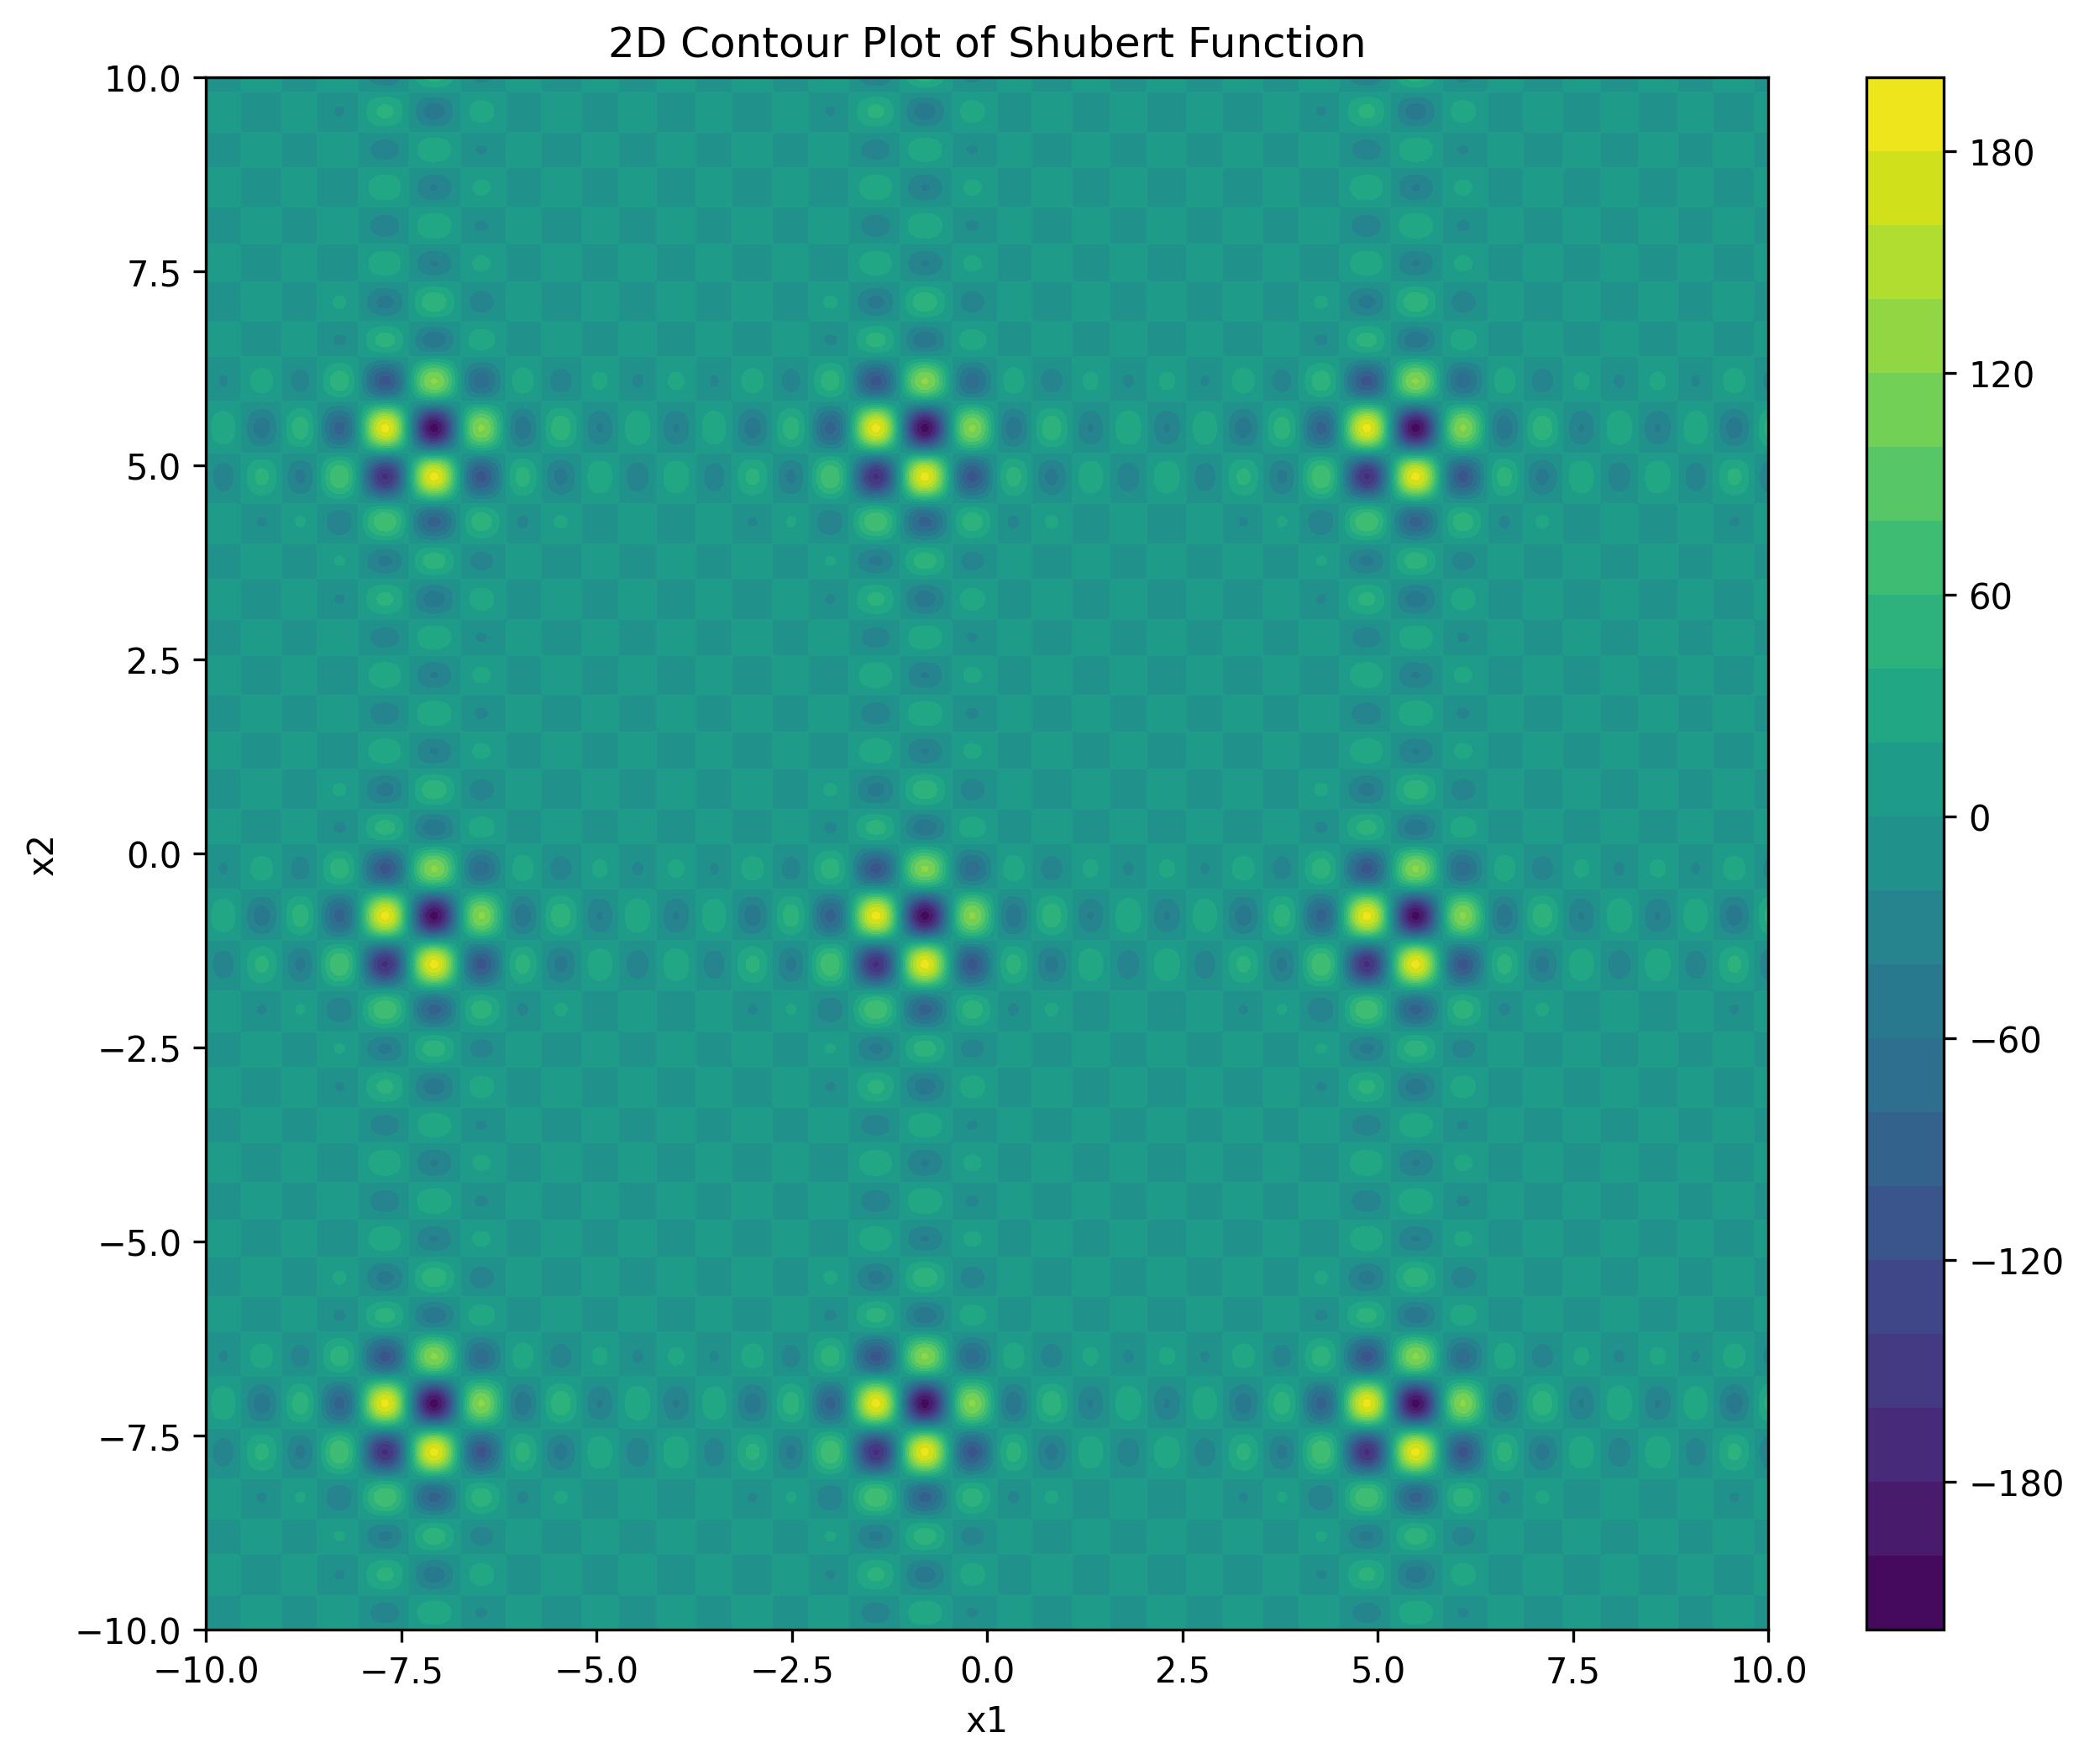
\includegraphics[width=\linewidth]{cec/shubert_2d.png}
		\caption{Dimensi 2}
		\label{fig:shubert-2d}
	\end{subfigure}
	\hfill
	\begin{subfigure}[b]{0.4\textwidth}
		\centering
		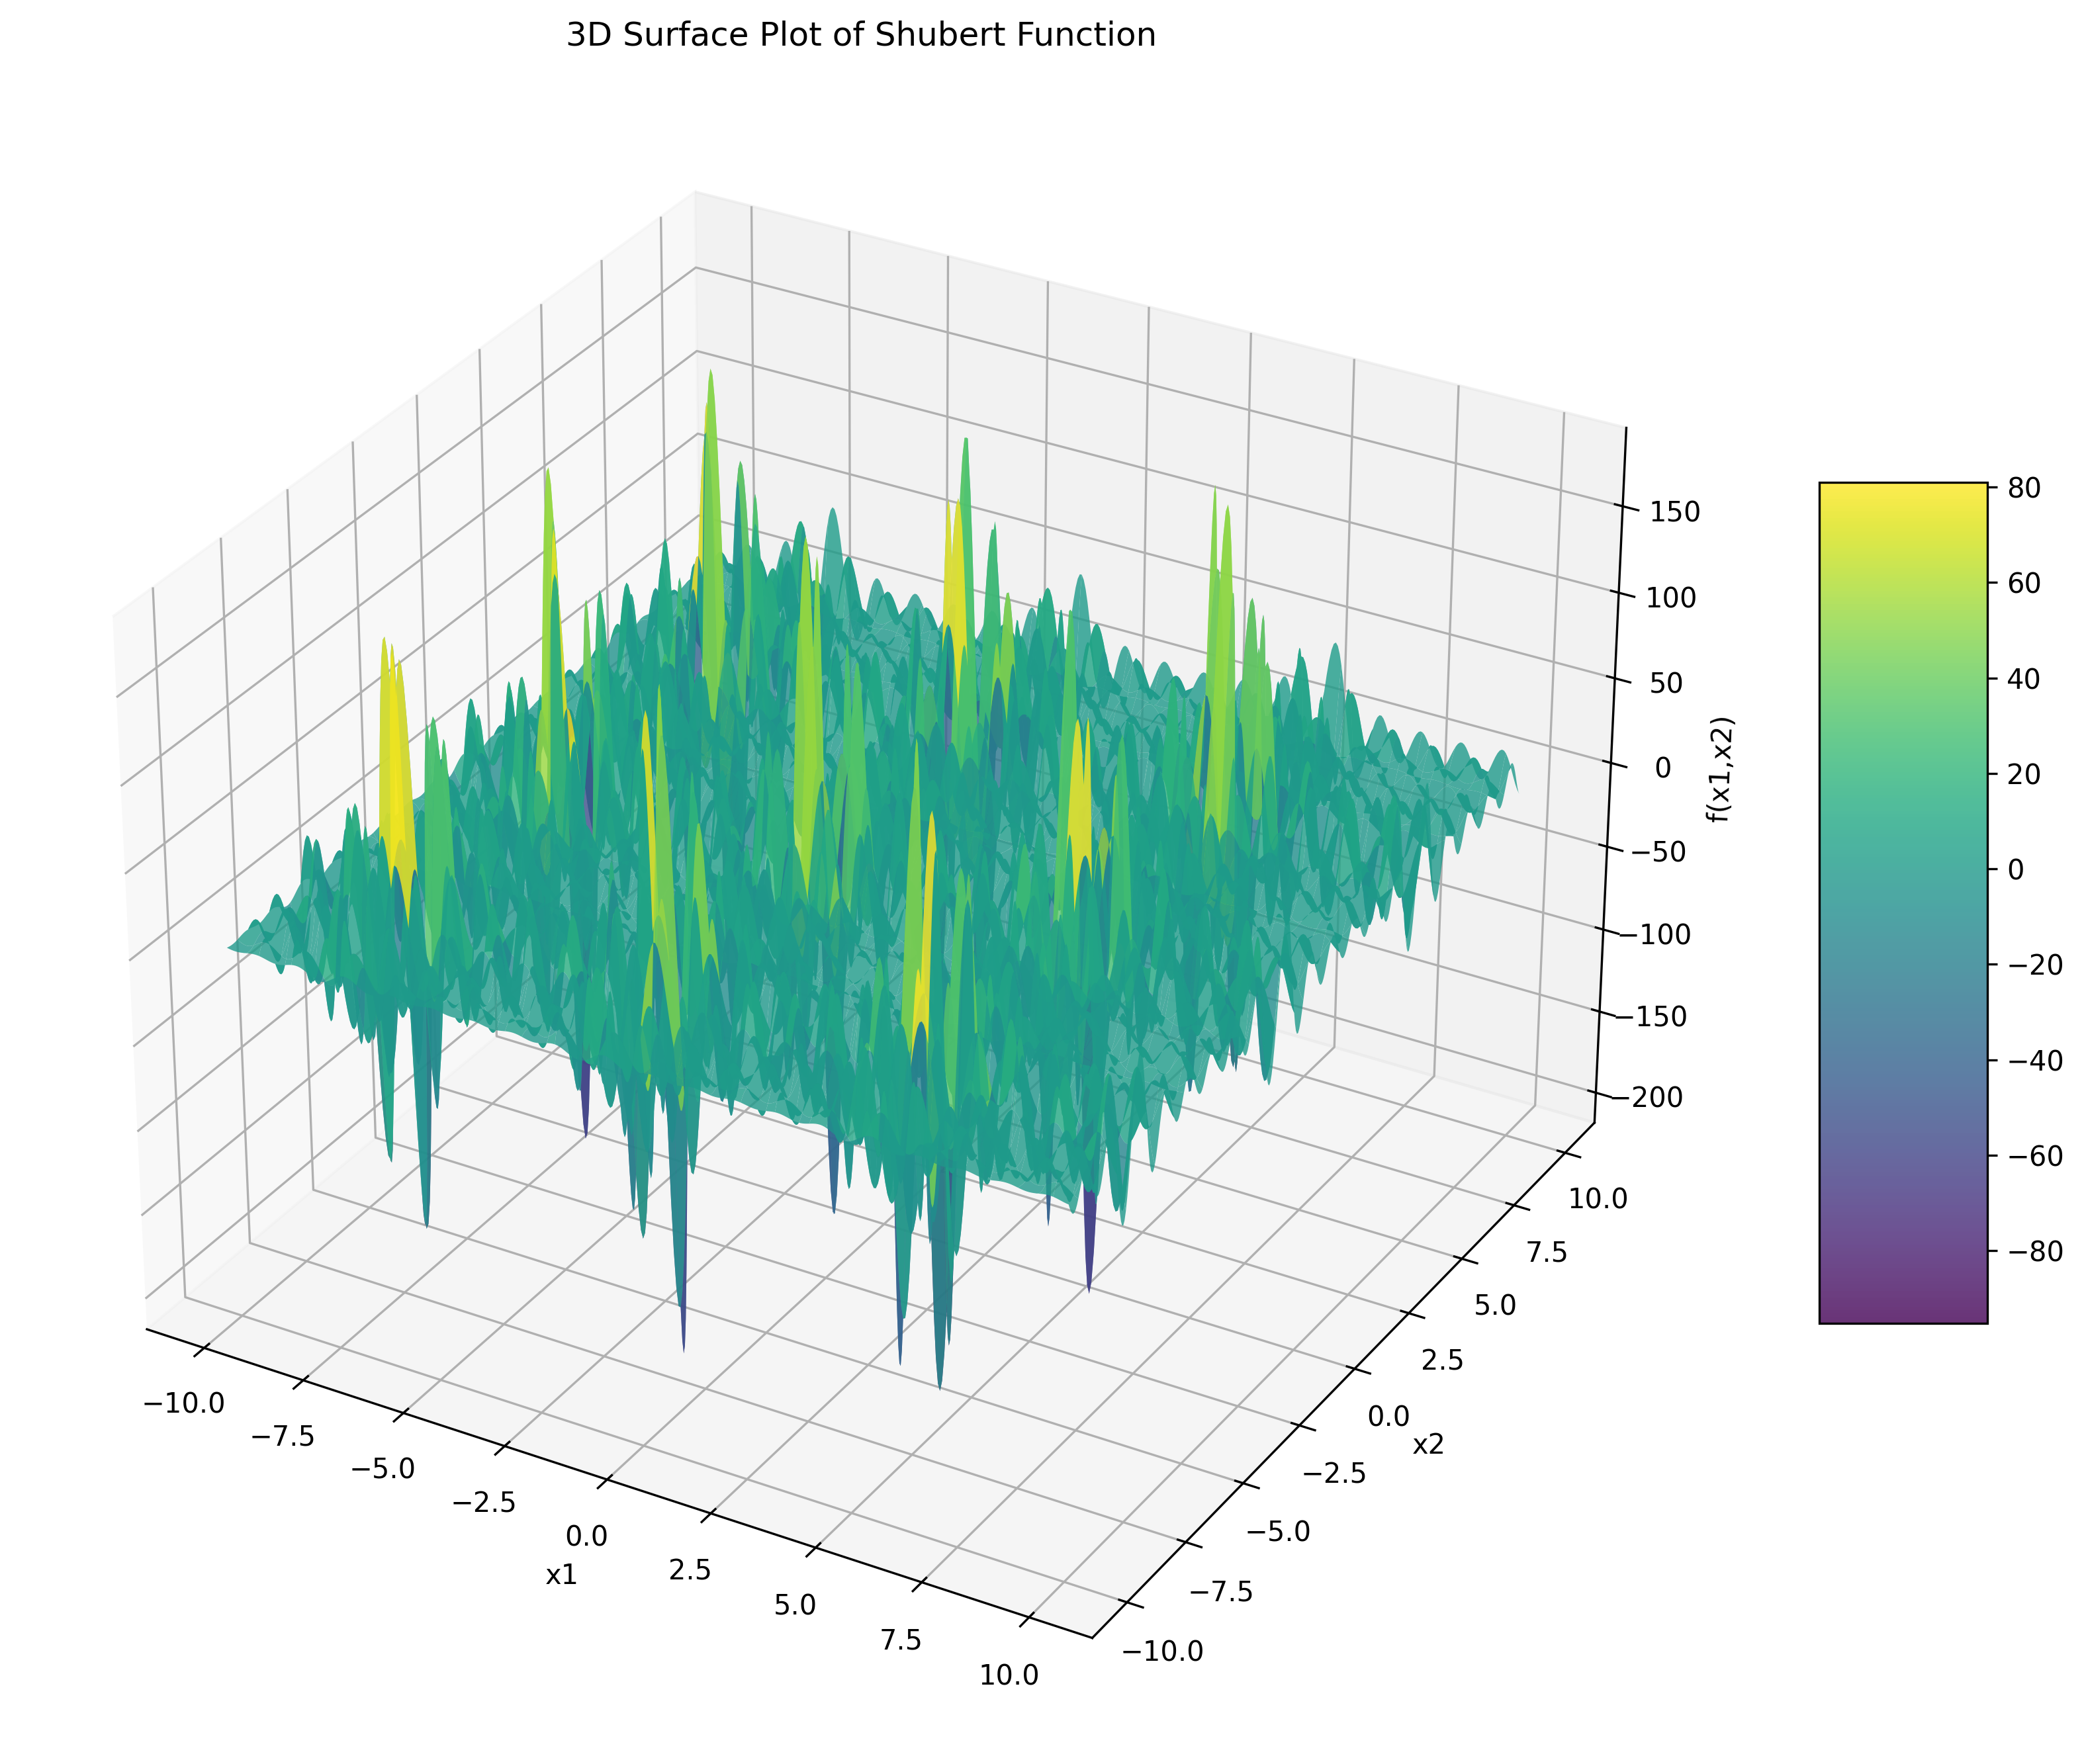
\includegraphics[width=\linewidth]{cec/shubert_3d.png}
		\caption{Dimensi 3}
		\label{fig:shubert-3d}
	\end{subfigure}
	\caption{Tampilan grafik fungsi Shubert pada dimensi dua (\cref{fig:shubert-2d}) dan tiga (\cref{fig:shubert-3d})}
	\label{fig:shubert}
\end{figure}
\begin{equation}
  f_{\text{Shubert}}(\mathrm{x})=-\prod_{i=1}^{D}\sum_{j=i}^{5}j\cos\left[\left(j+1 \right)z_i+j  \right]  +f_{\text{bias}}
\end{equation}

\subsubsection*{Sphere}
\noindent Properti:
\begin{packed_item}
  \item unimodal
  \item convex
  \item separable
\end{packed_item}
\begin{figure}[H]
	\centering
	\begin{subfigure}[b]{0.4\textwidth}
		\centering
		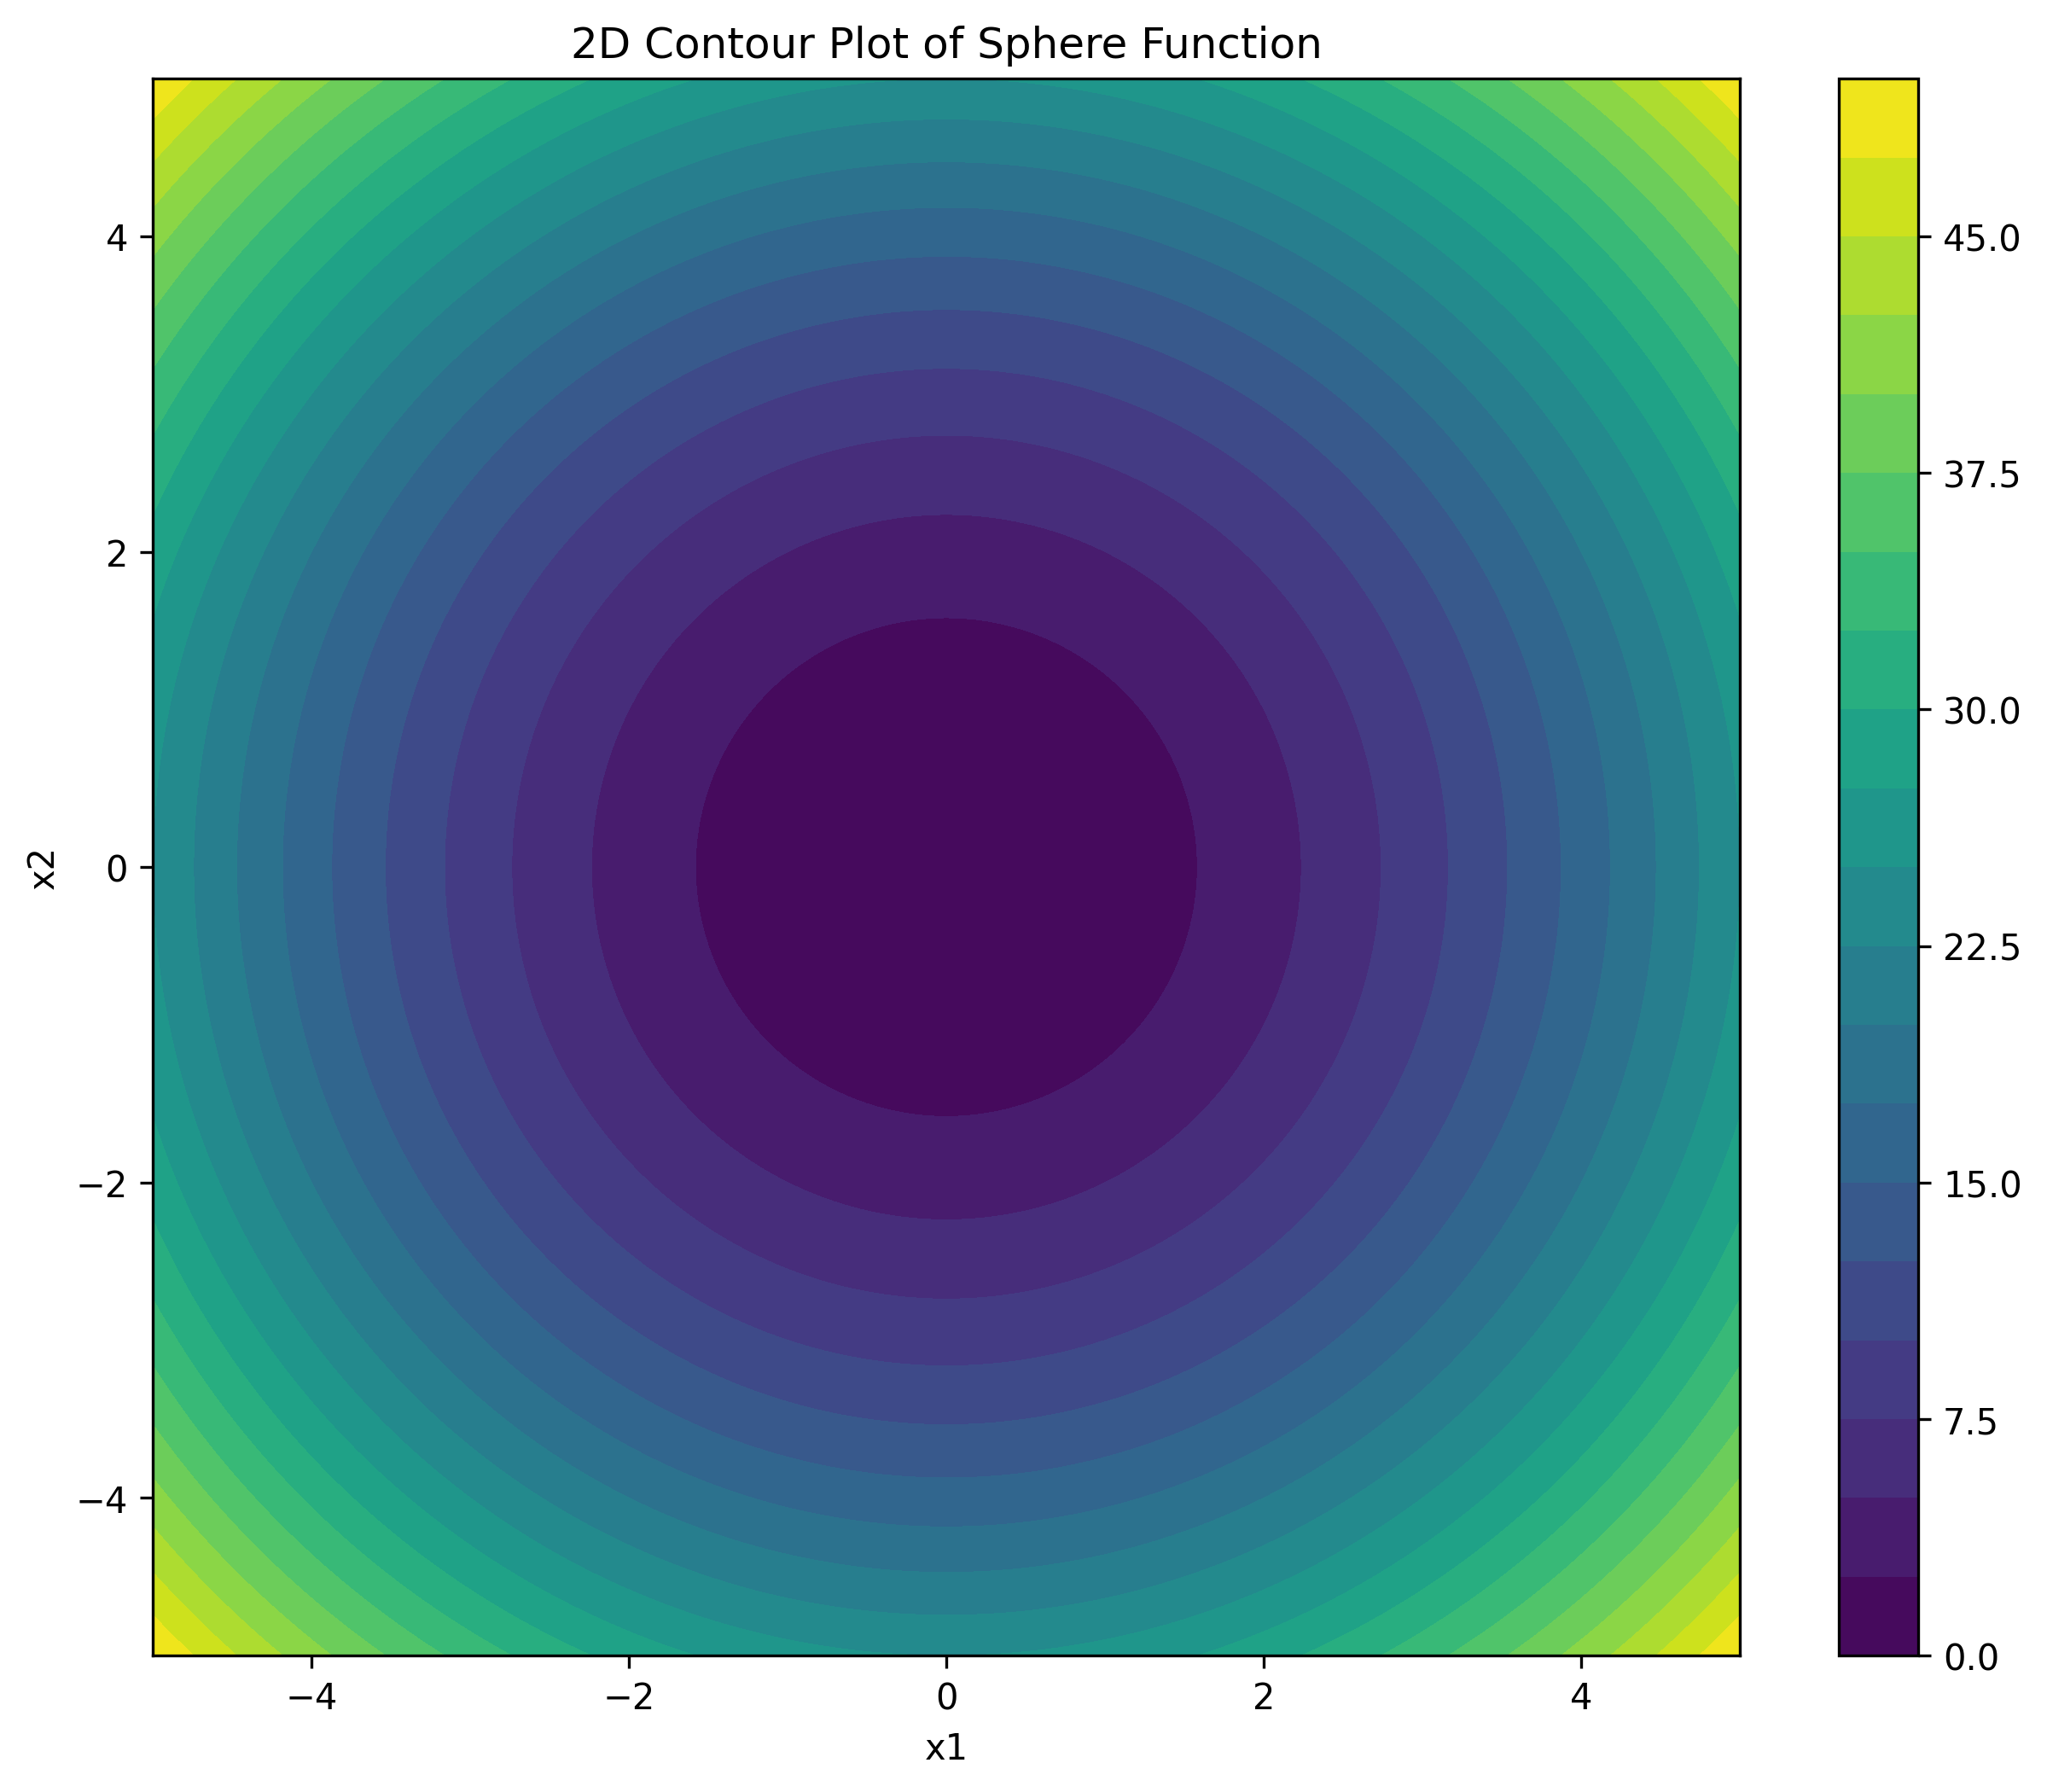
\includegraphics[width=\linewidth]{cec/sphere_2d.png}
		\caption{Dimensi 2}
		\label{fig:sphere-2d}
	\end{subfigure}
	\hfill
	\begin{subfigure}[b]{0.4\textwidth}
		\centering
		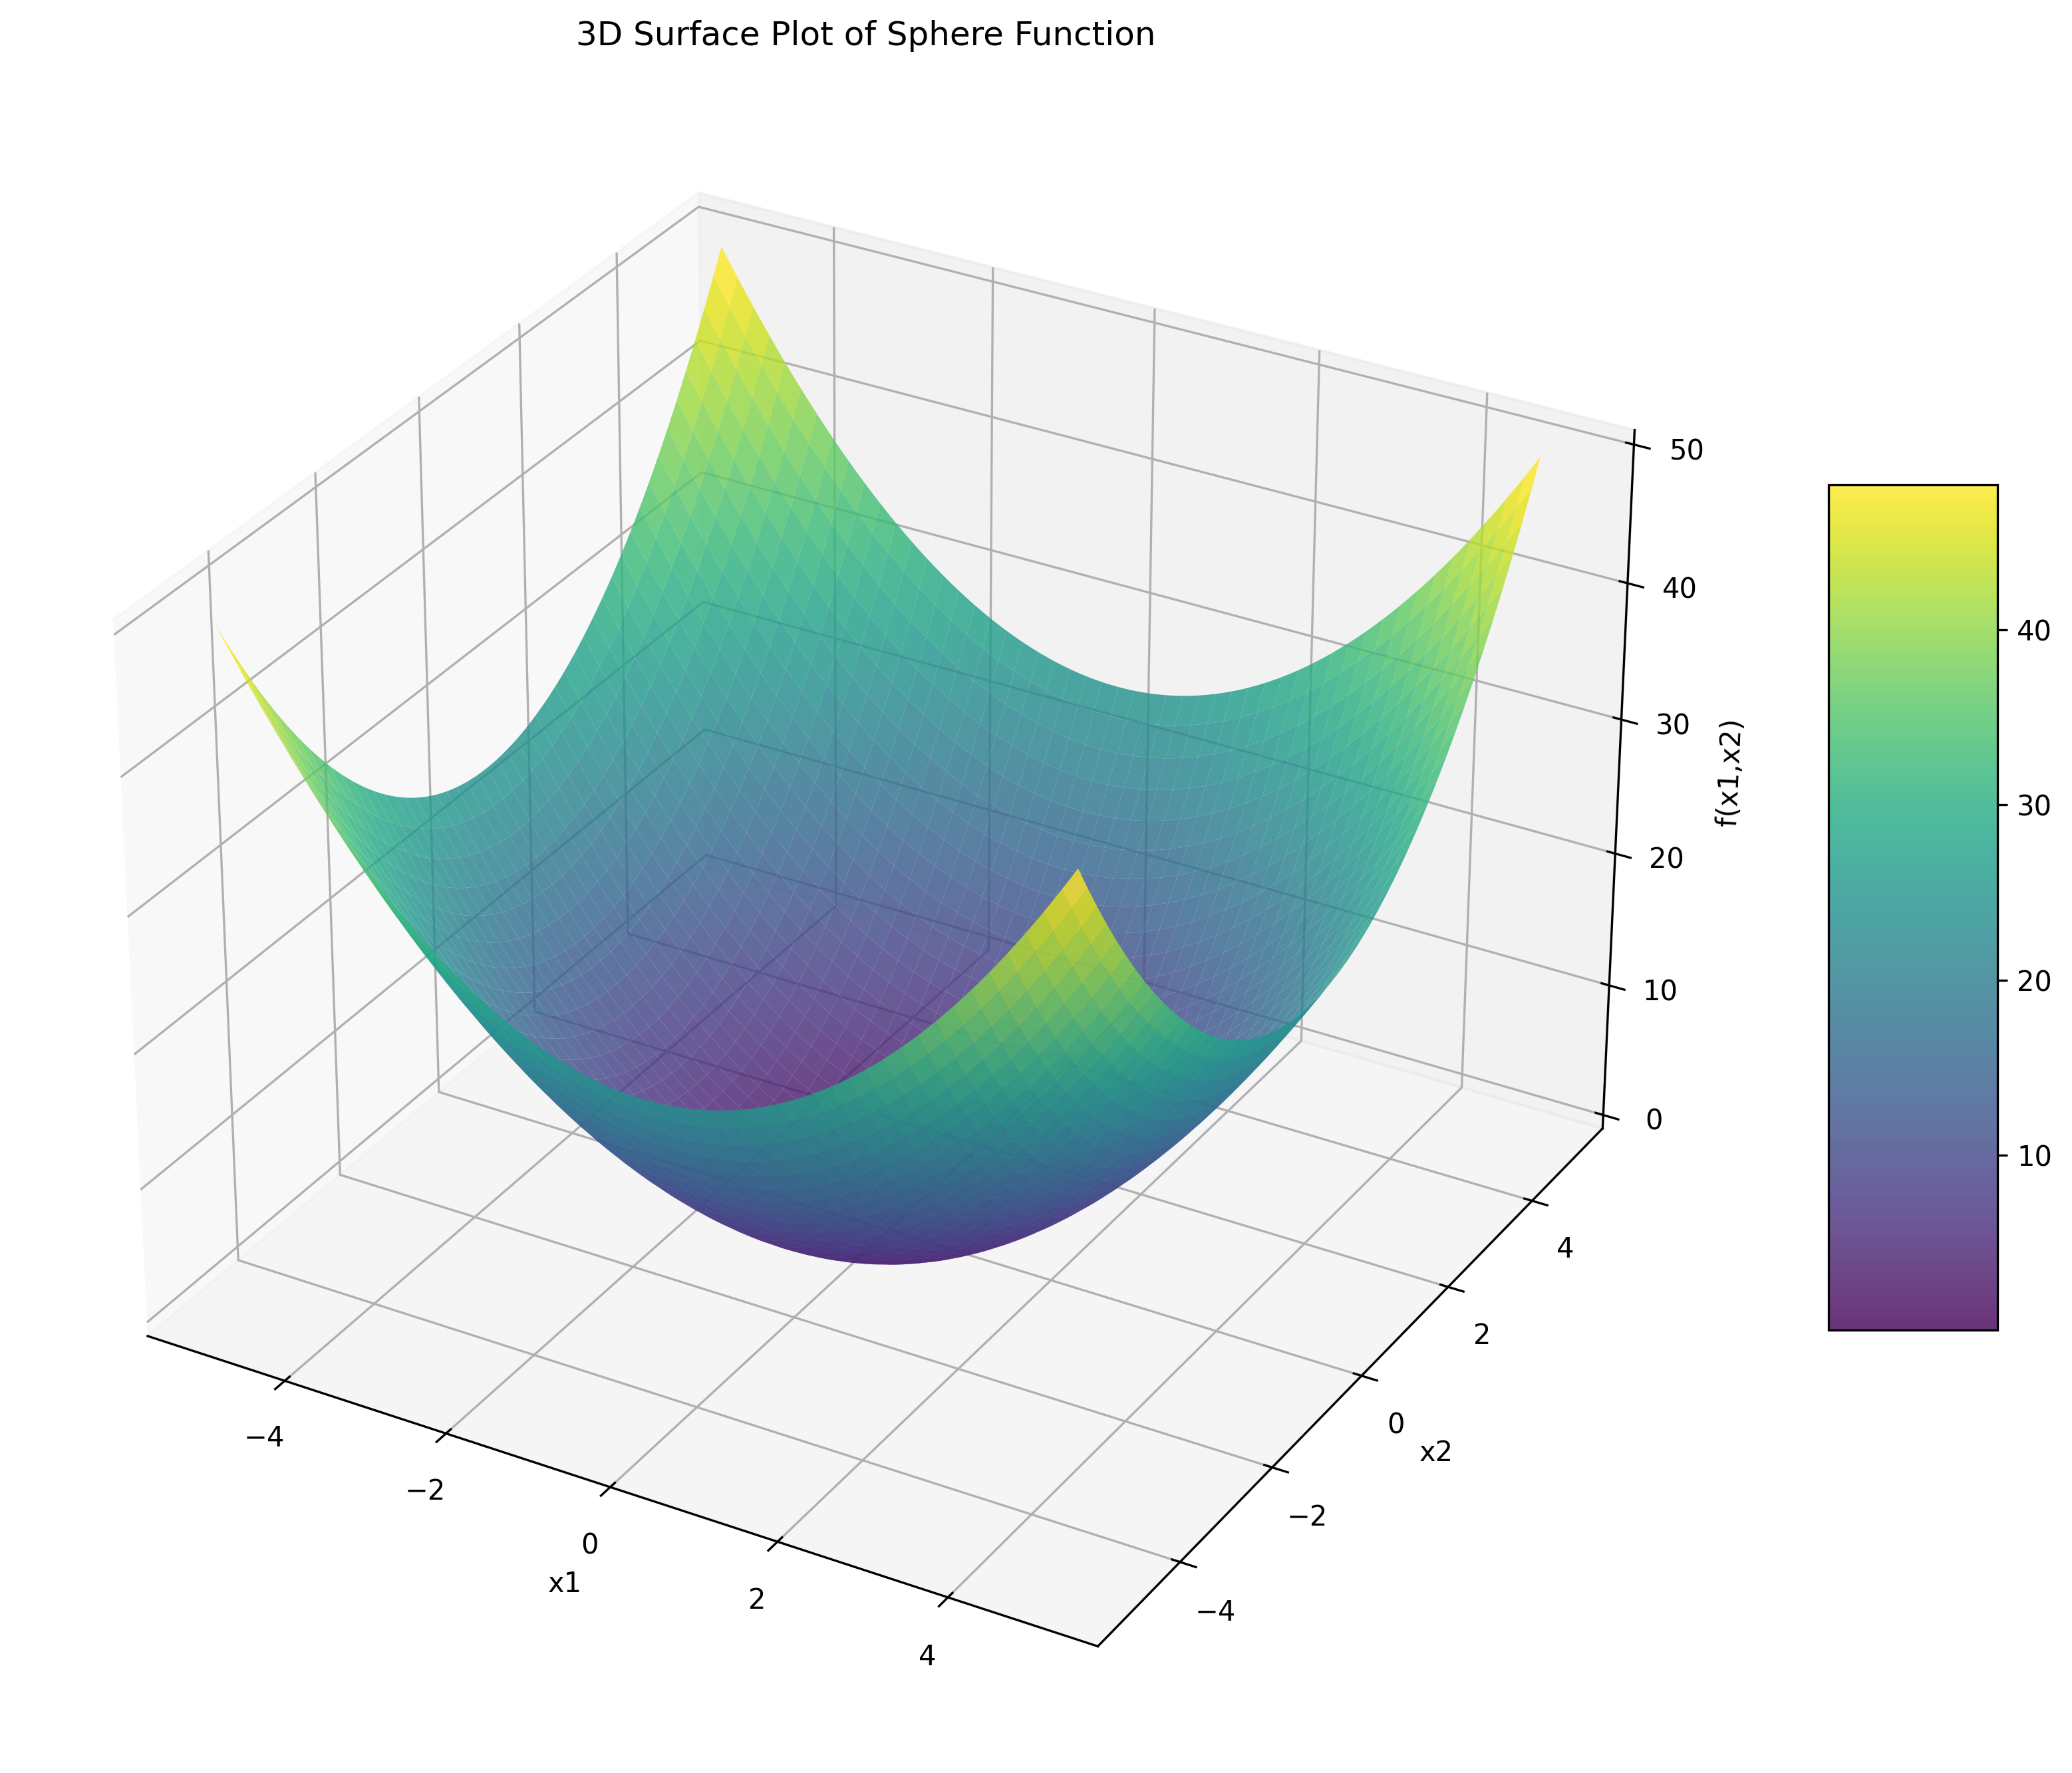
\includegraphics[width=\linewidth]{cec/sphere_3d.png}
		\caption{Dimensi 3}
		\label{fig:sphere-3d}
	\end{subfigure}
	\caption{Tampilan grafik fungsi Sphere pada dimensi dua (\cref{fig:sphere-2d}) dan tiga (\cref{fig:sphere-3d})}
	\label{fig:sphere}
\end{figure}
\begin{equation}
  f_{\text{Sphere}}(\mathrm{x})=\sum_{i=1}^{D}z_i^2+f_{\text{bias}}
\end{equation}

\subsubsection*{Step Function}
\noindent Properti:
\begin{packed_item}
  \item unimodal
  \item convex
\end{packed_item}
\begin{figure}[H]
	\centering
	\begin{subfigure}[b]{0.4\textwidth}
		\centering
		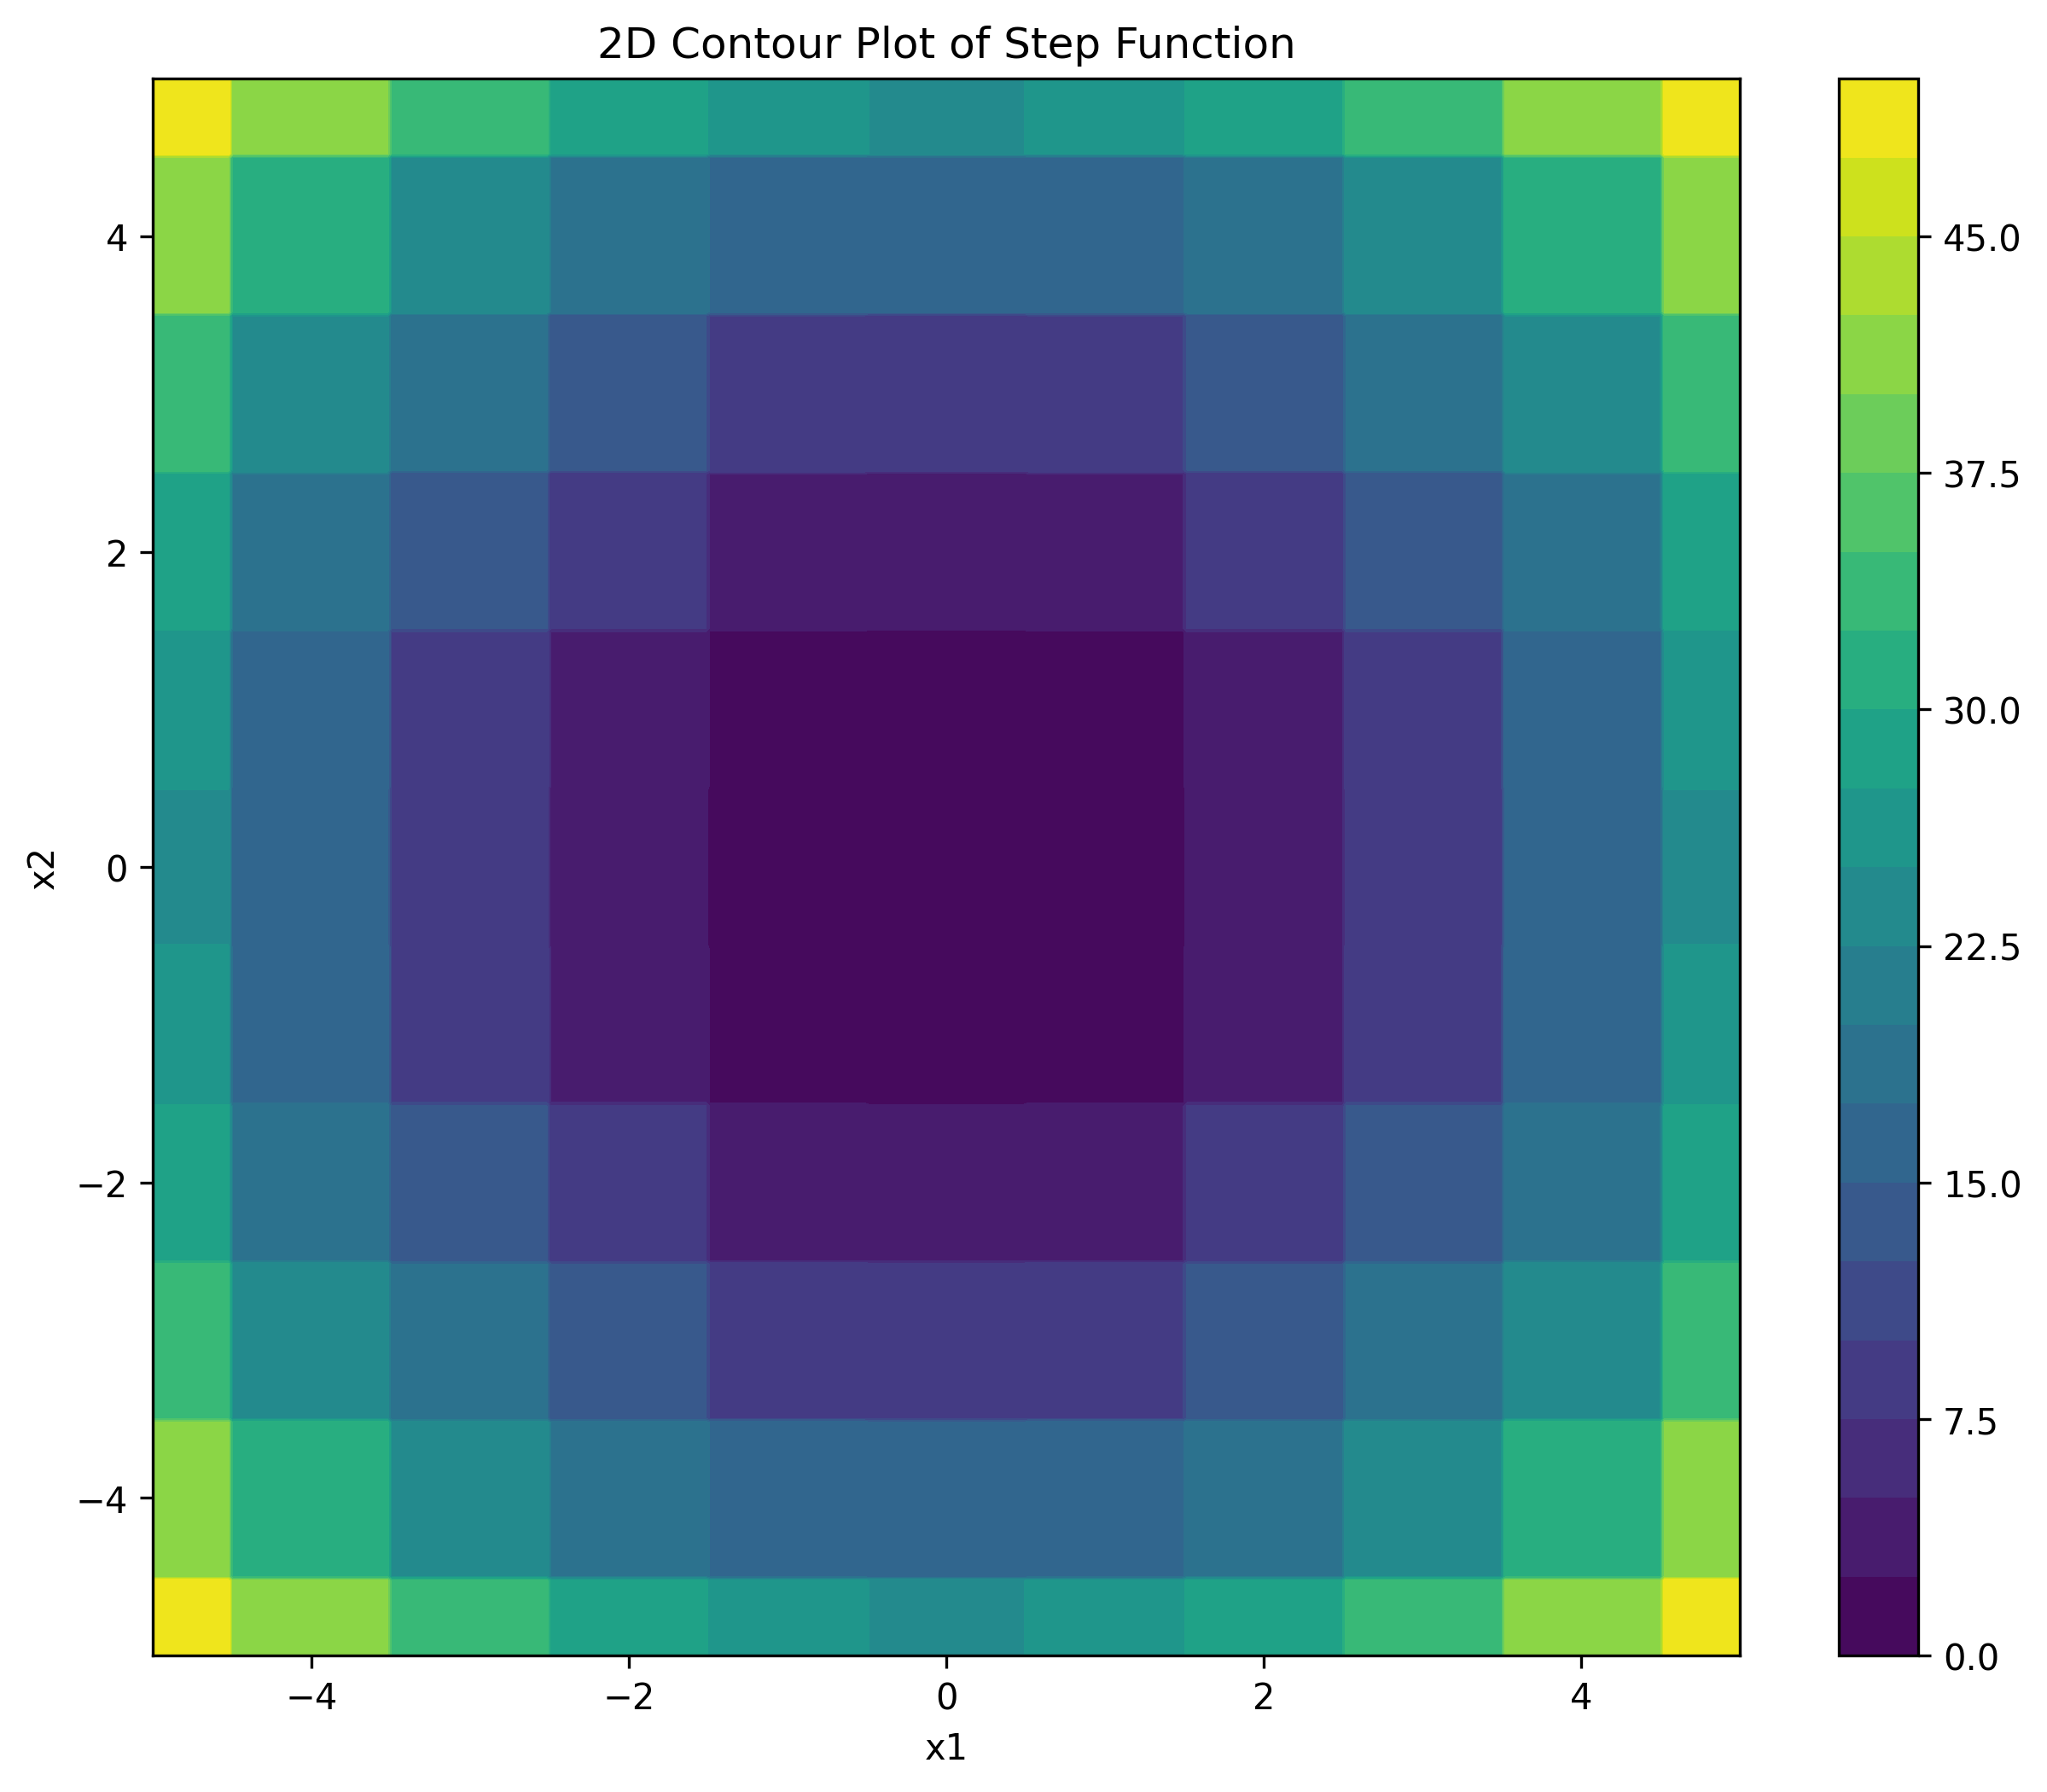
\includegraphics[width=\linewidth]{cec/step_function_2d.png}
		\caption{Dimensi 2}
		\label{fig:step-2d}
	\end{subfigure}
	\hfill
	\begin{subfigure}[b]{0.4\textwidth}
		\centering
		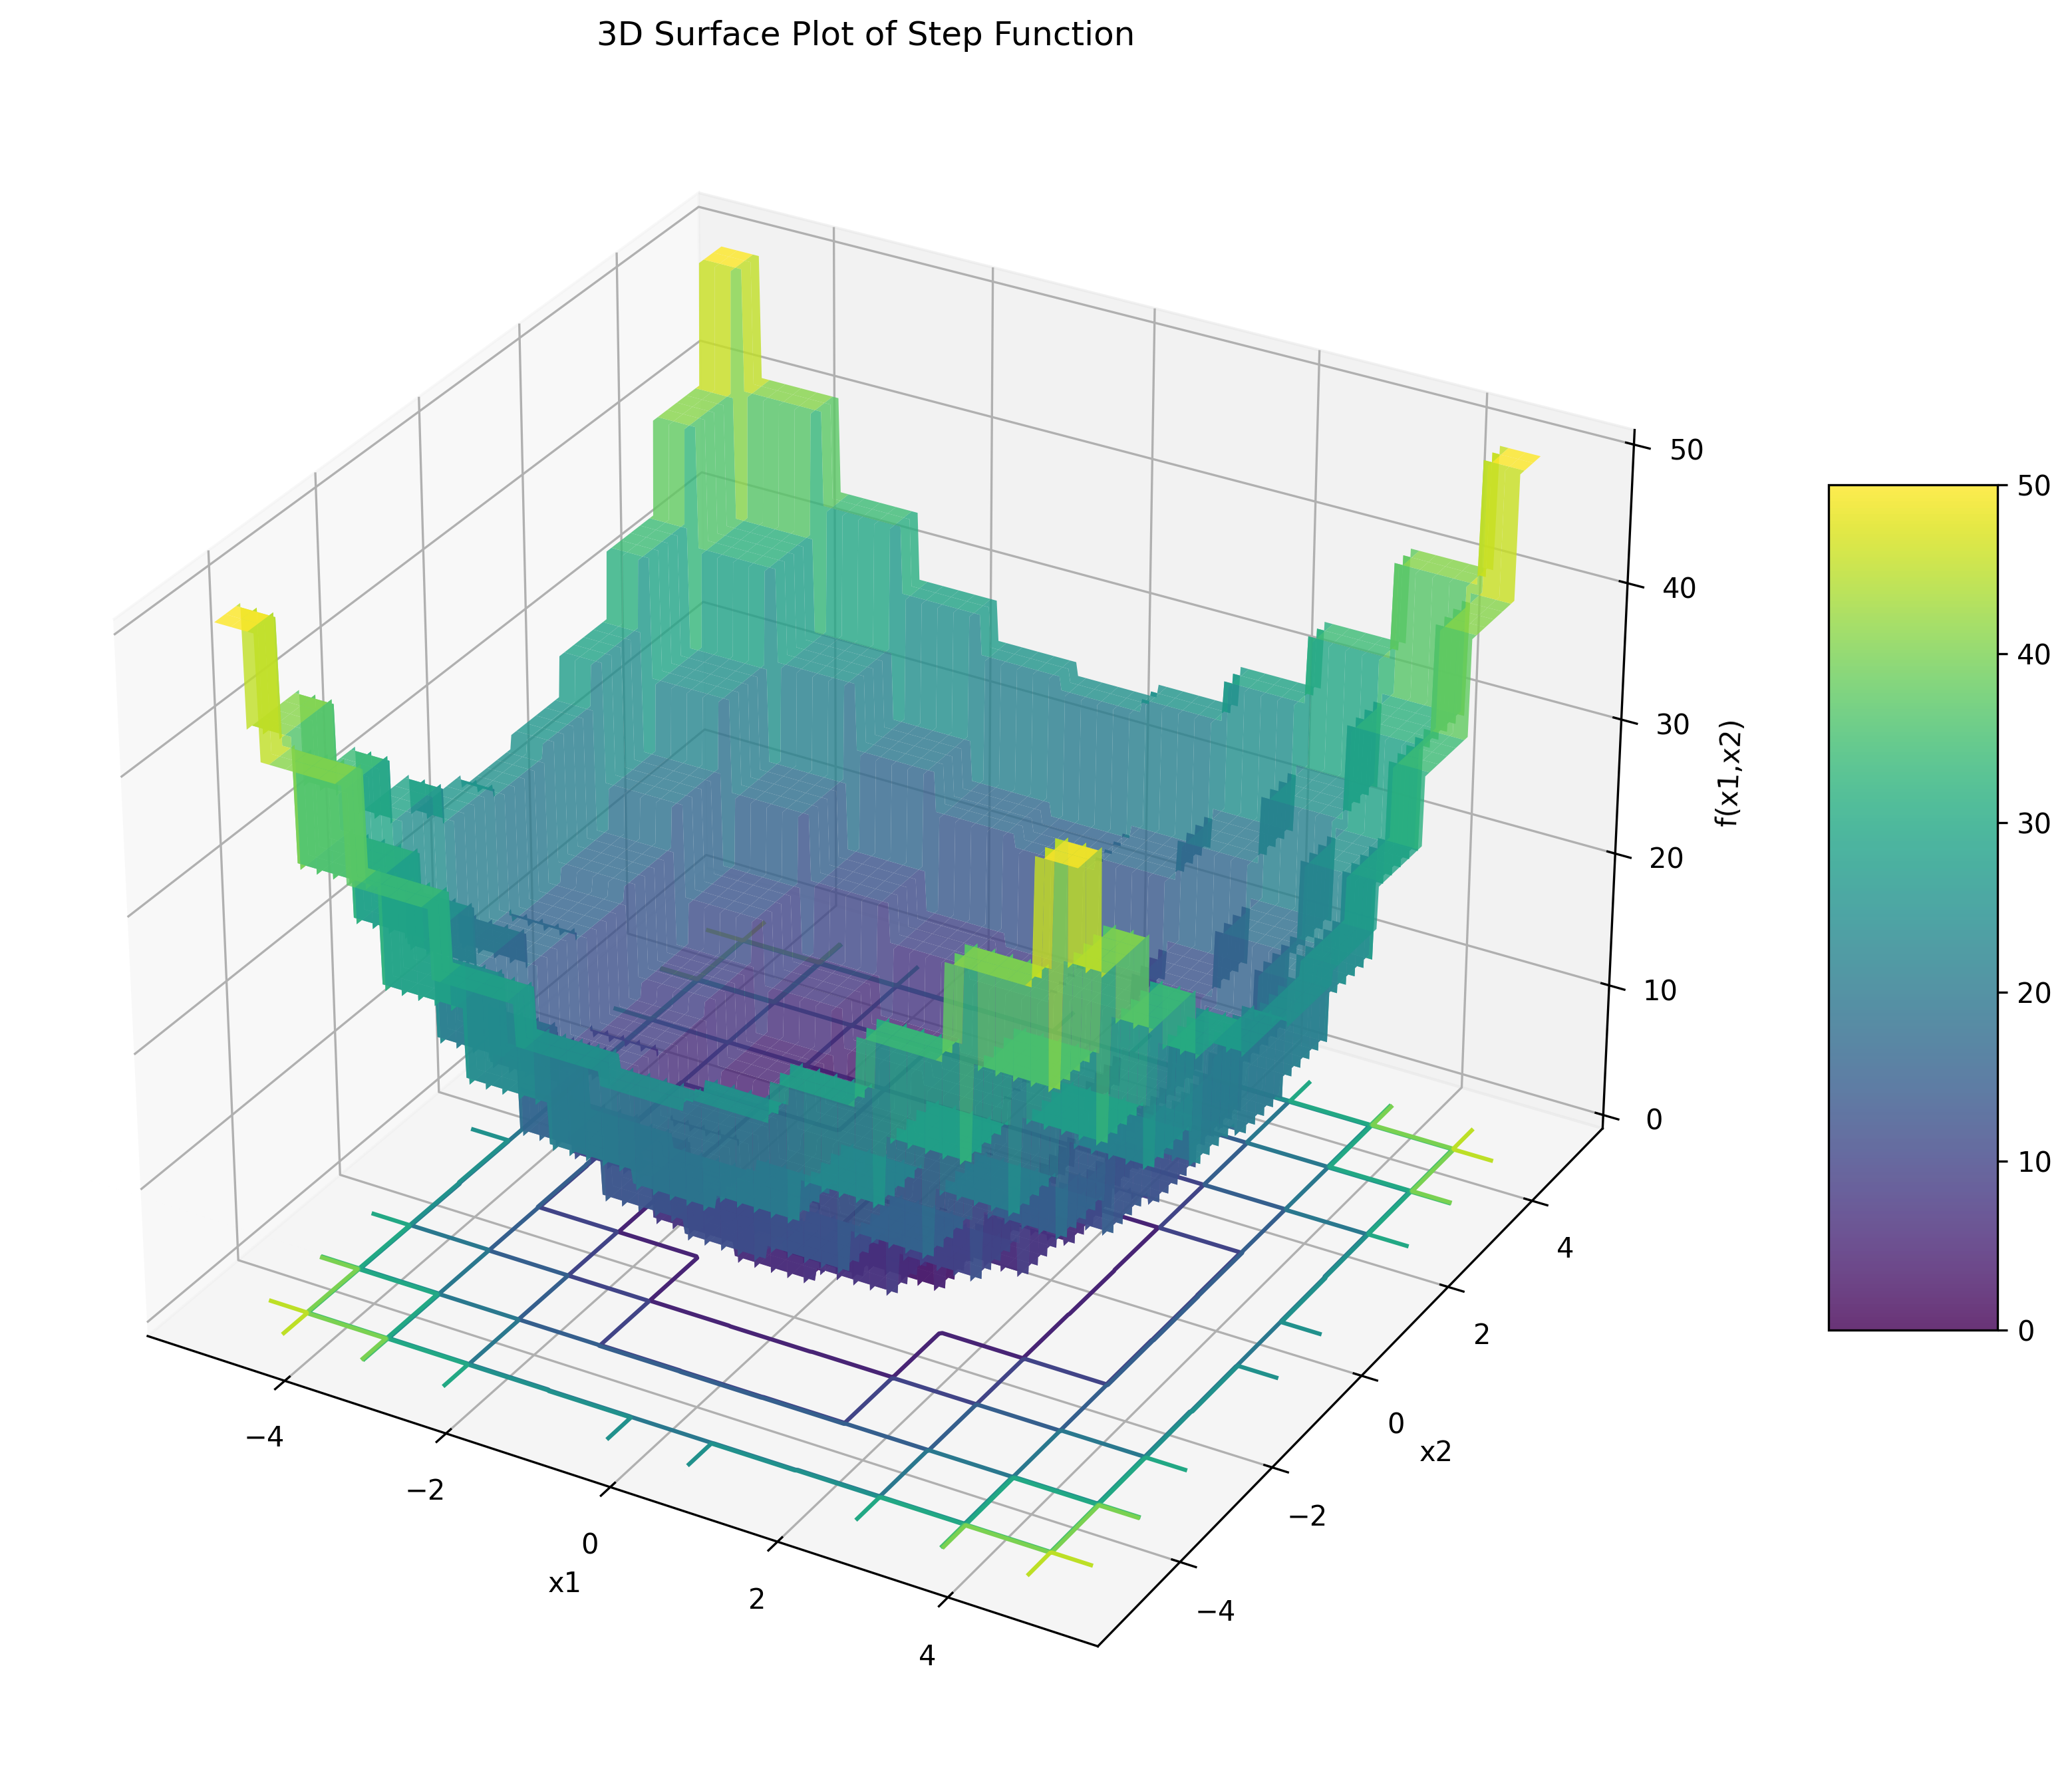
\includegraphics[width=\linewidth]{cec/step_function_3d.png}
		\caption{Dimensi 3}
		\label{fig:step-3d}
	\end{subfigure}
	\caption{Tampilan grafik fungsi Step Function pada dimensi dua (\cref{fig:step-2d}) dan tiga (\cref{fig:step-3d})}
	\label{fig:step-function}
\end{figure}
\begin{equation}
  f_{\text{Step function}}(\mathrm{x})=\sum_{i=1}^{D}\left(\left\lfloor z_i + 0.5 \right\rfloor \right)^2+f_{\text{bias}}
\end{equation}

\subsubsection*{Vincent}
\noindent Properti:
\begin{packed_item}
  \item multimodal
  \item non-convex
\end{packed_item}
\begin{figure}[H]
	\centering
	\begin{subfigure}[b]{0.4\textwidth}
		\centering
		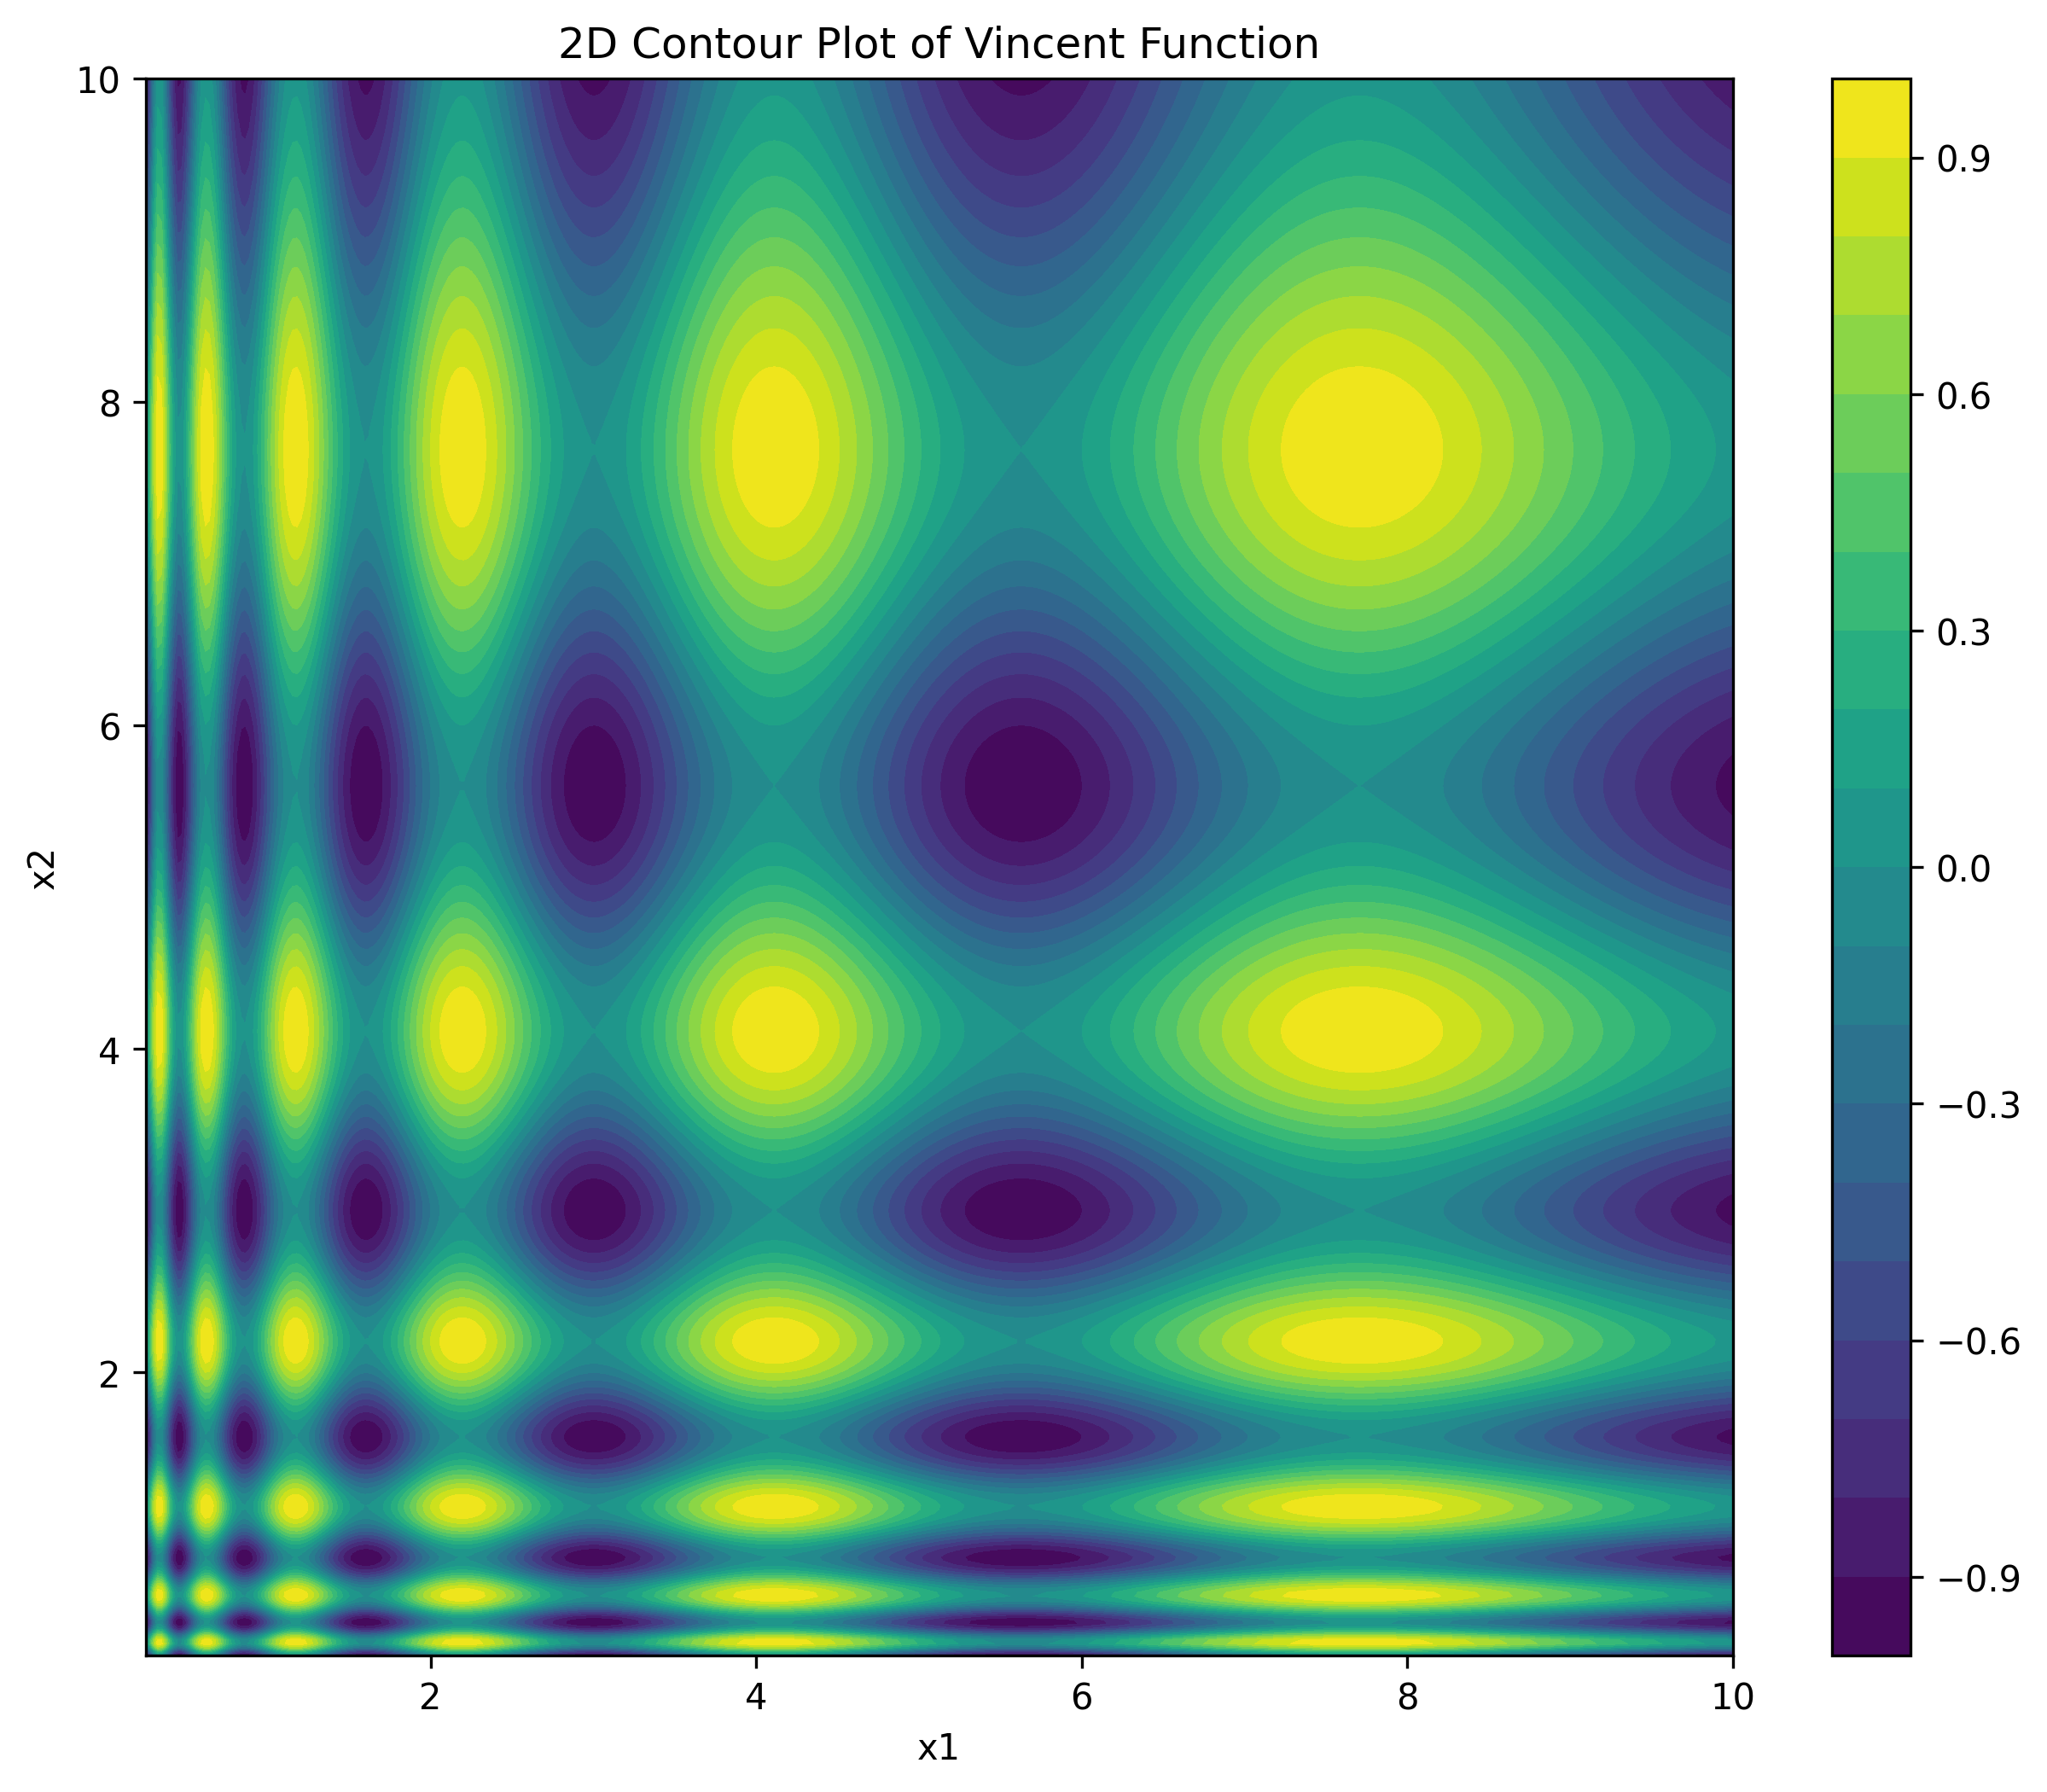
\includegraphics[width=\linewidth]{cec/vincent_2d.png}
		\caption{Dimensi 2}
		\label{fig:vincent-2d}
	\end{subfigure}
	\hfill
	\begin{subfigure}[b]{0.4\textwidth}
		\centering
		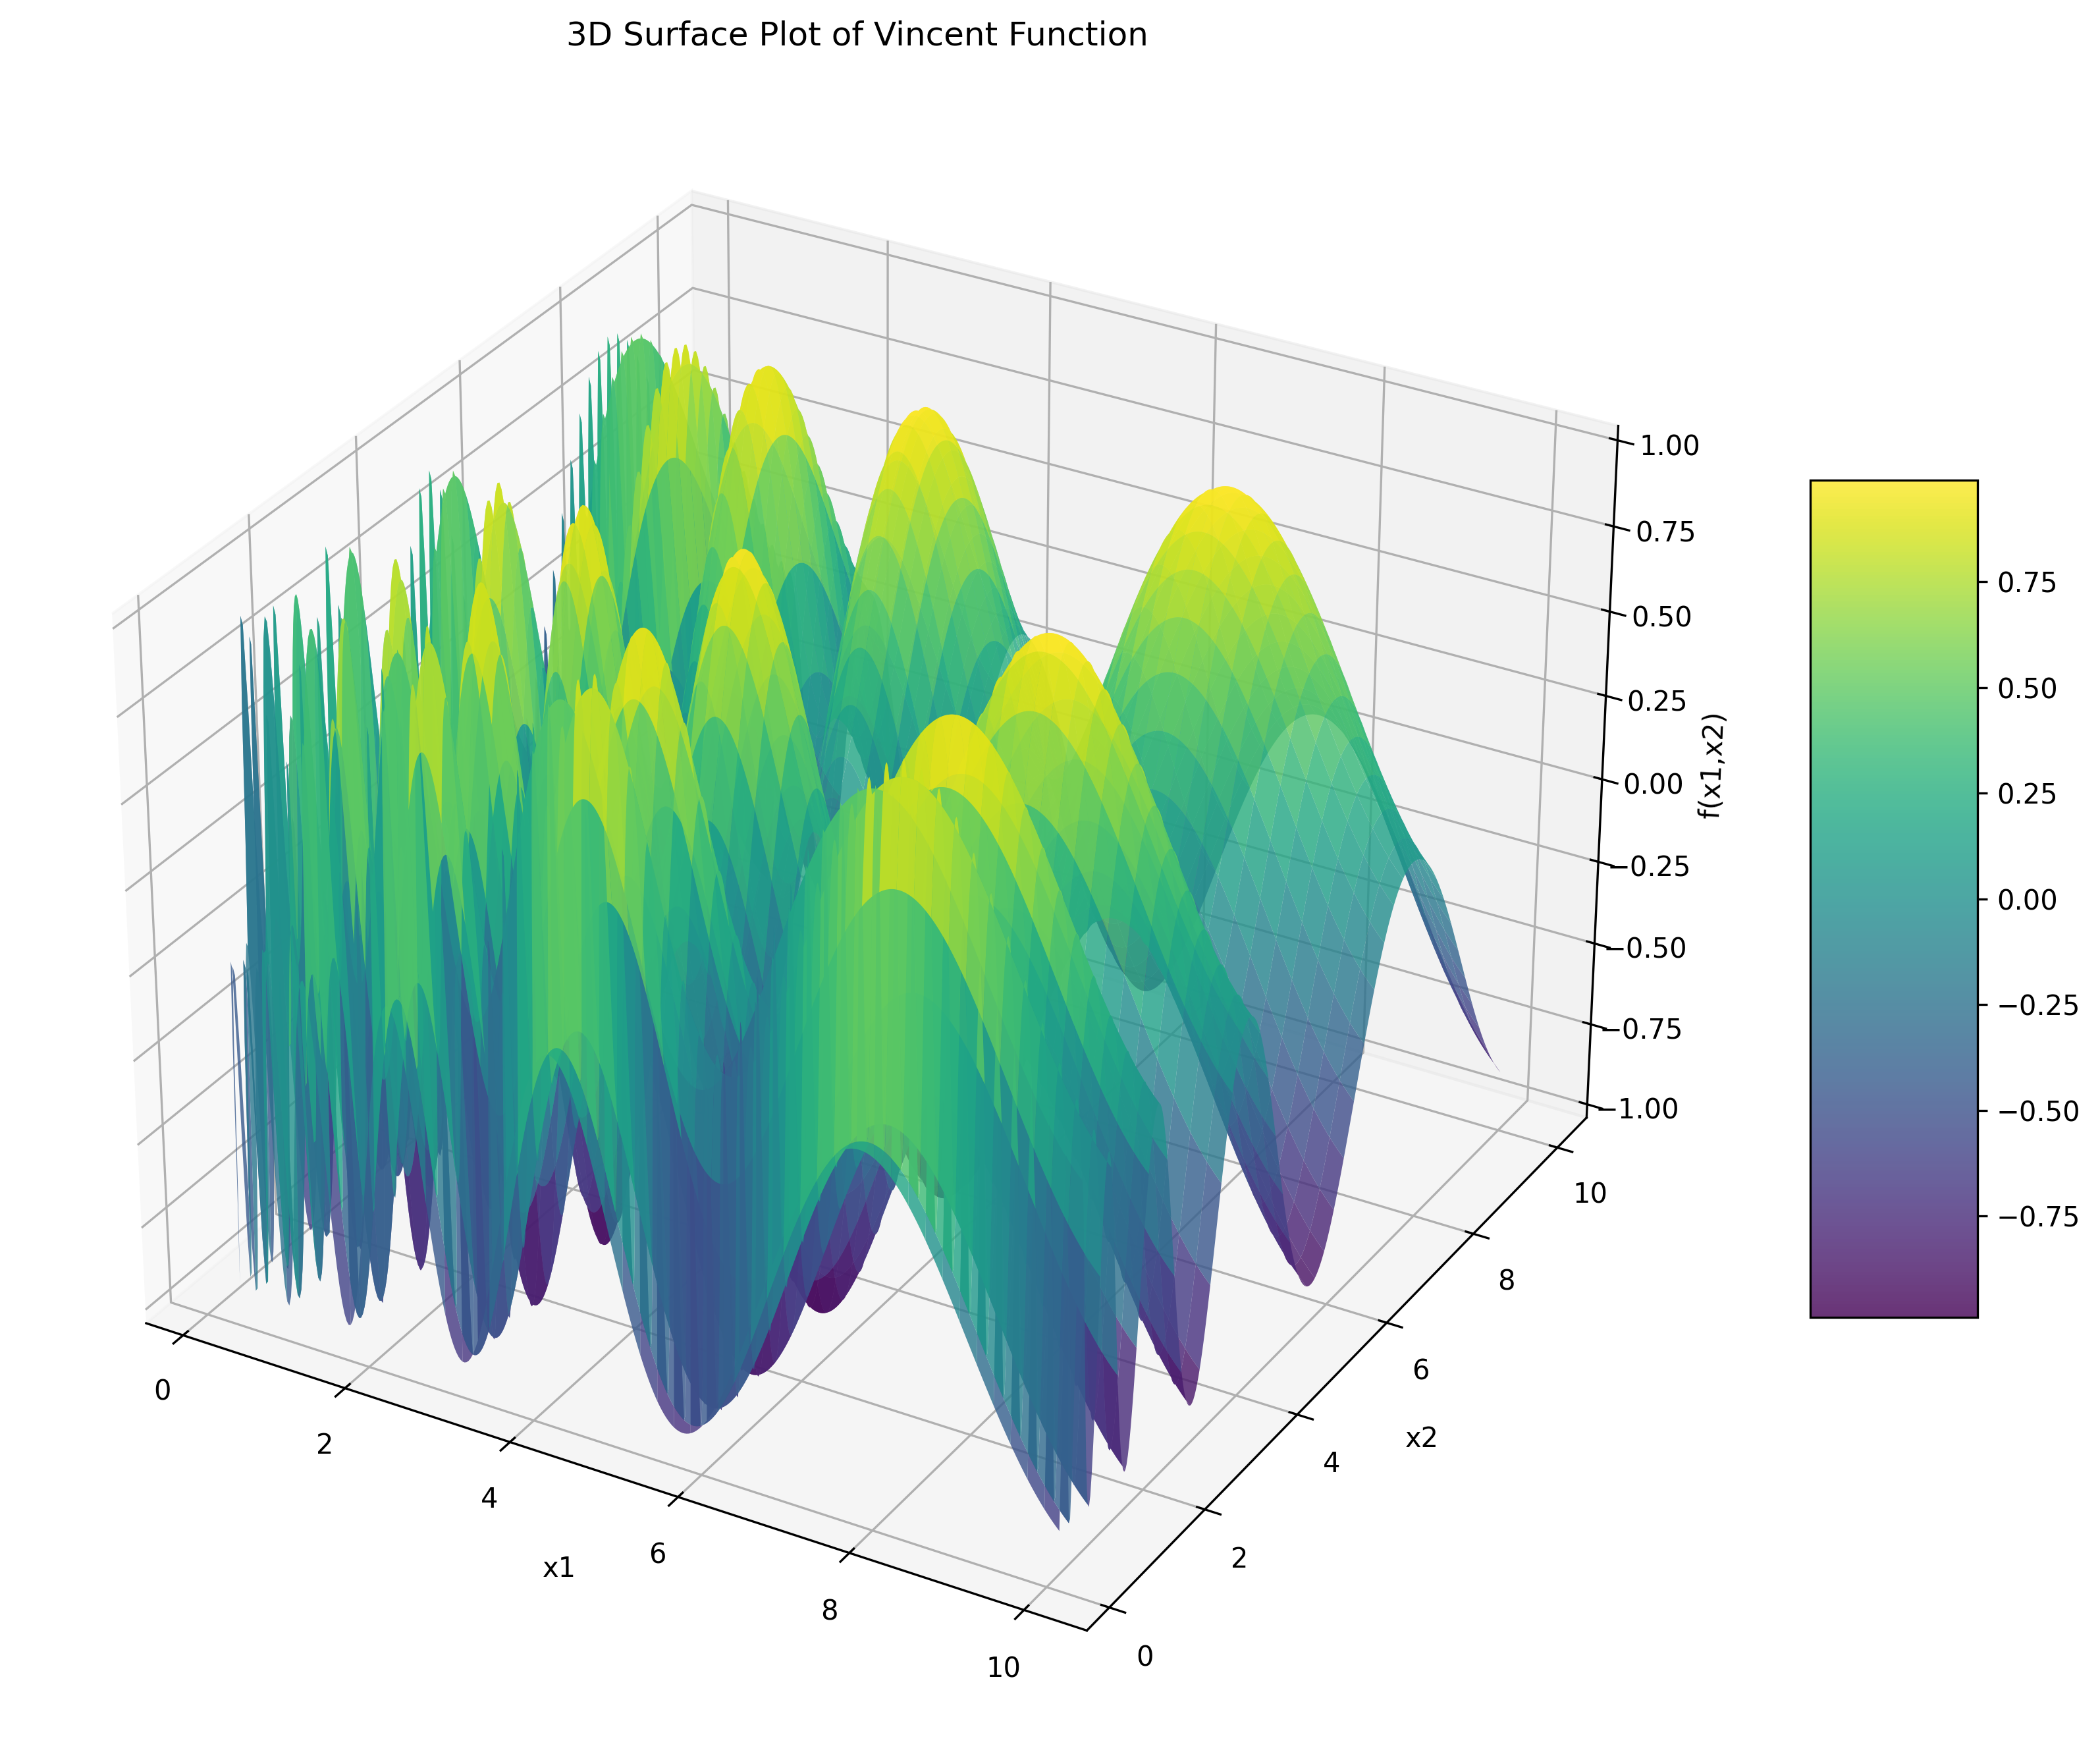
\includegraphics[width=\linewidth]{cec/vincent_3d.png}
		\caption{Dimensi 3}
		\label{fig:vincent-3d}
	\end{subfigure}
	\caption{Tampilan grafik fungsi Vincent pada dimensi dua (\cref{fig:vincent-2d}) dan tiga (\cref{fig:vincent-3d})}
	\label{fig:vincent}
\end{figure}
\begin{equation}
  f_{\text{Vincent}}(\mathrm{x})=\frac{1}{D}\sum_{i=1}^{D}\sin\left(10 \log\left(z_i \right)  \right) +f_{\text{bias}}
\end{equation}

\subsubsection*{Weierstrass}
\noindent Properti:
\begin{packed_item}
  \item multimodal
  \item non-convex
  \item non-separable
  \item Continuous but differentiable only on a set of points
\end{packed_item}
\begin{figure}[H]
	\centering
	\begin{subfigure}[b]{0.4\textwidth}
		\centering
		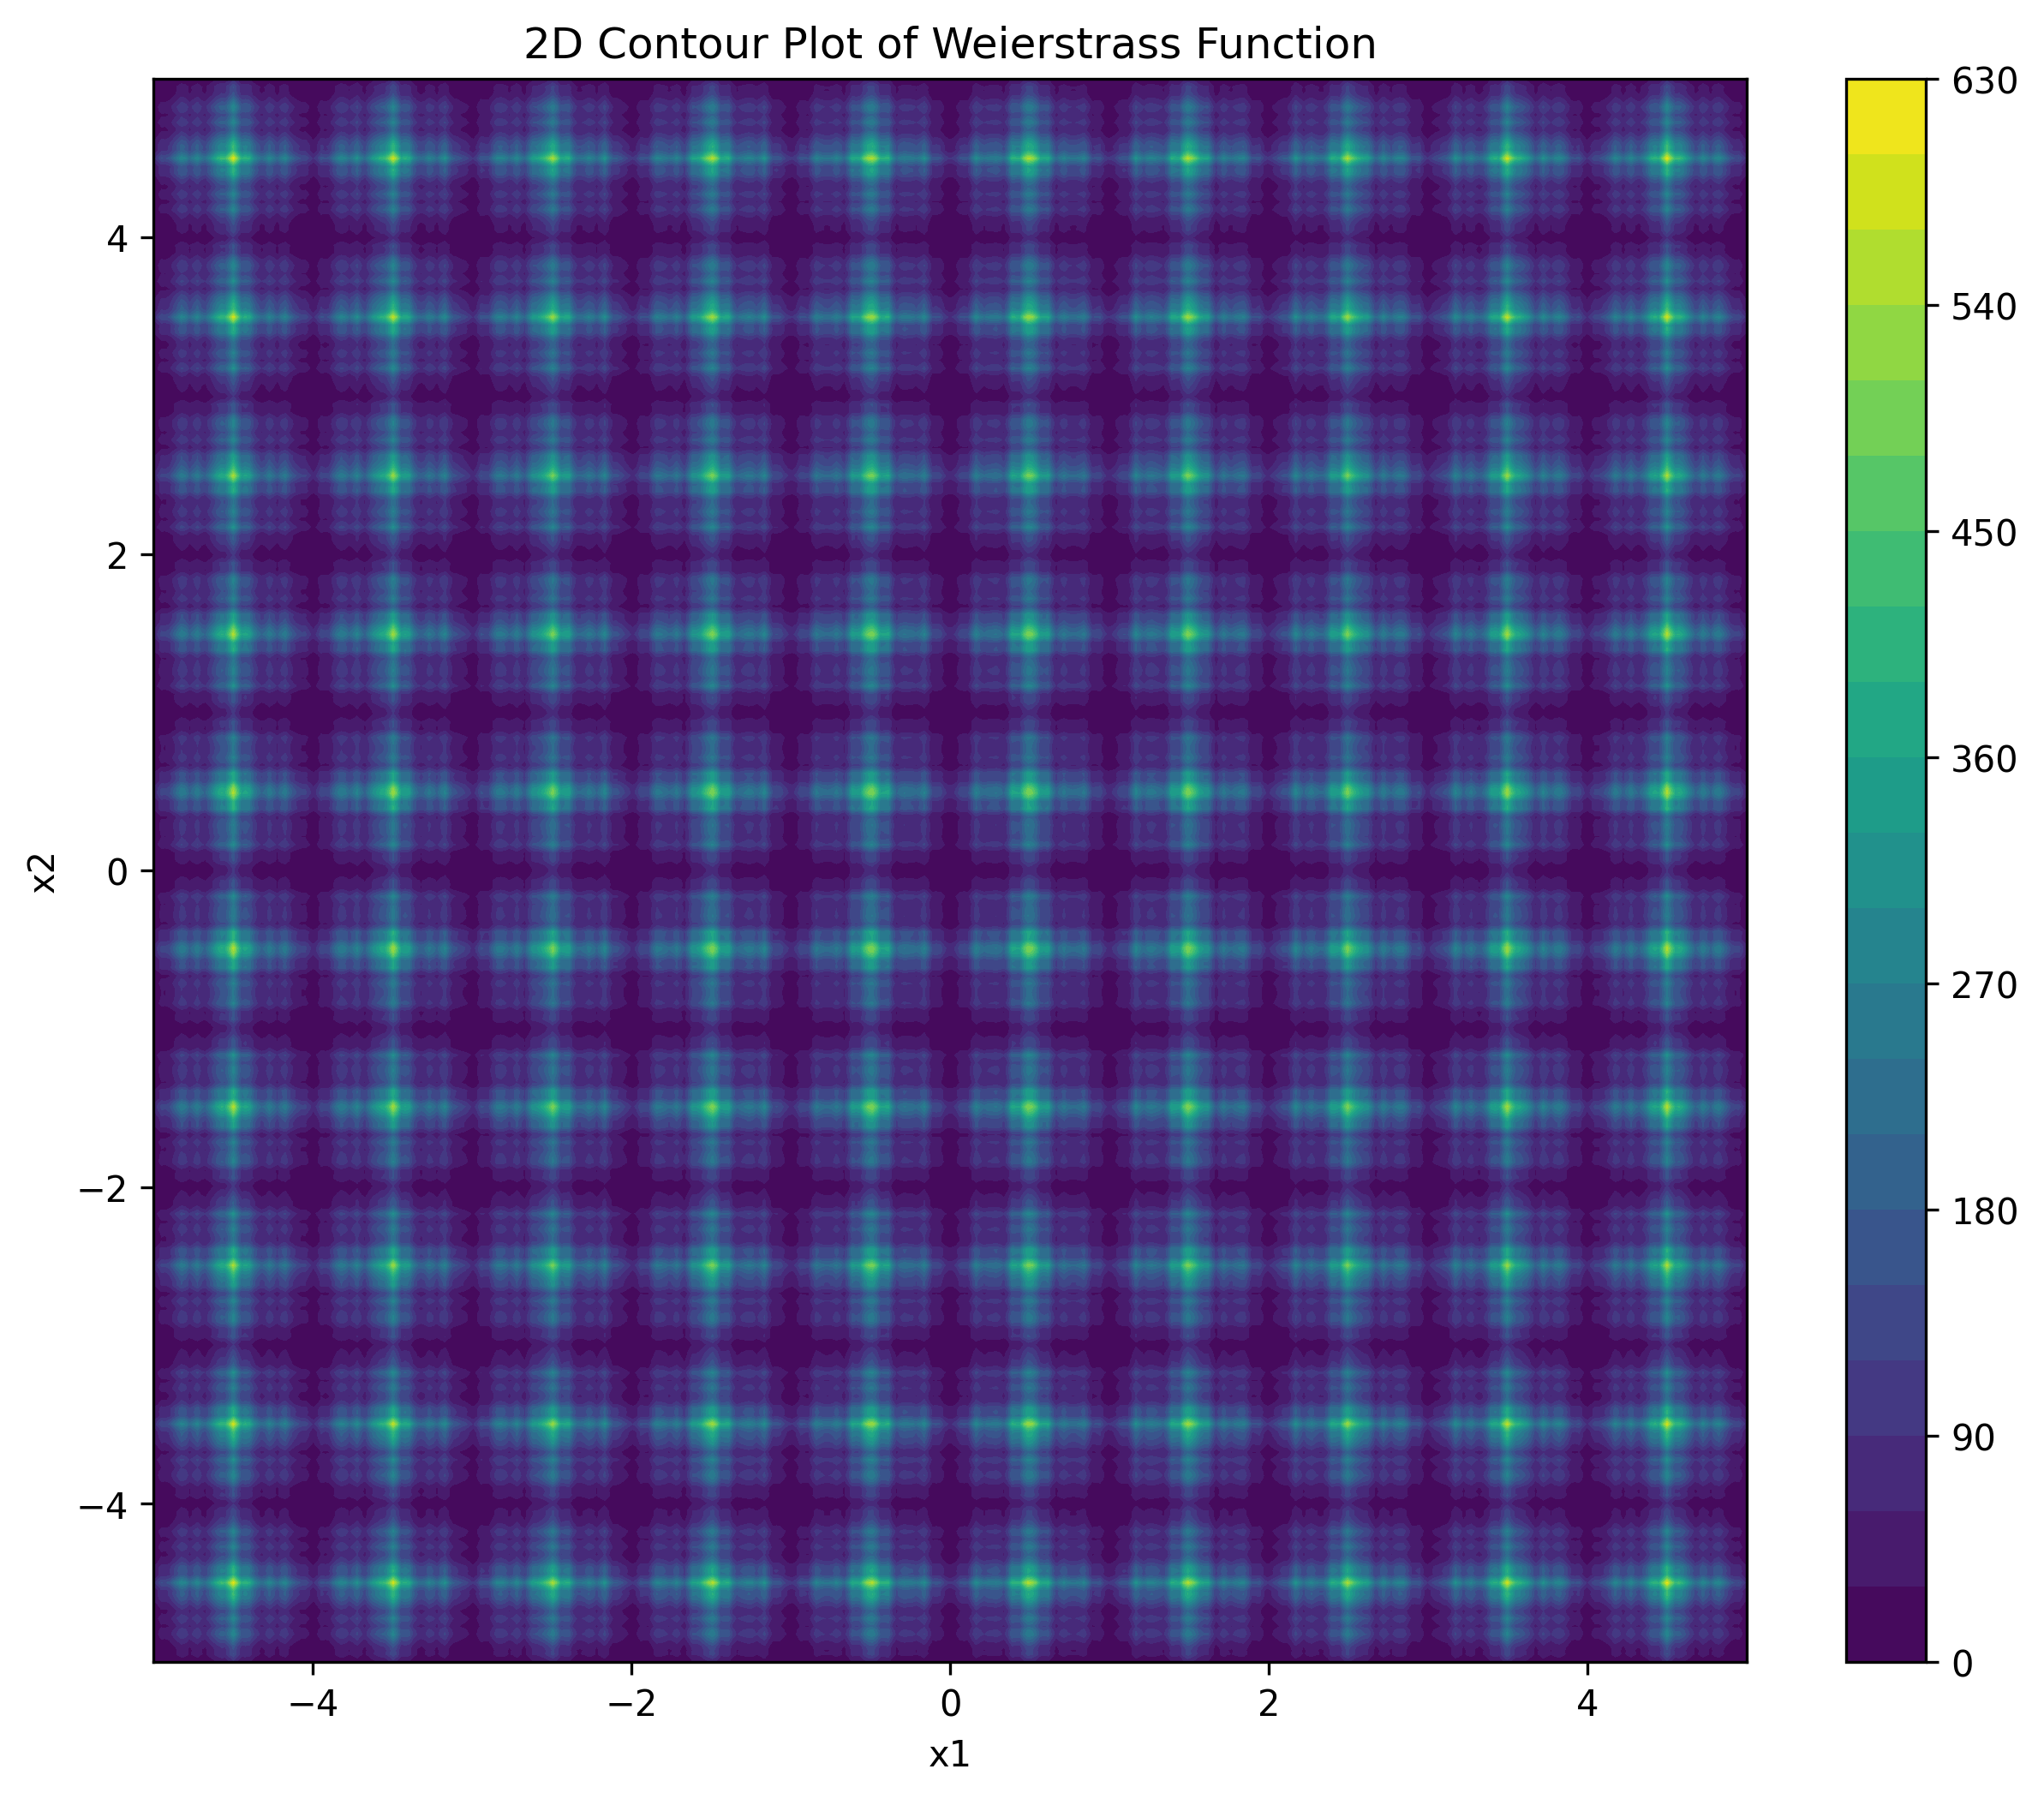
\includegraphics[width=\linewidth]{cec/weierstrass_2d.png}
		\caption{Dimensi 2}
		\label{fig:weierstrass-2d}
	\end{subfigure}
	\hfill
	\begin{subfigure}[b]{0.4\textwidth}
		\centering
		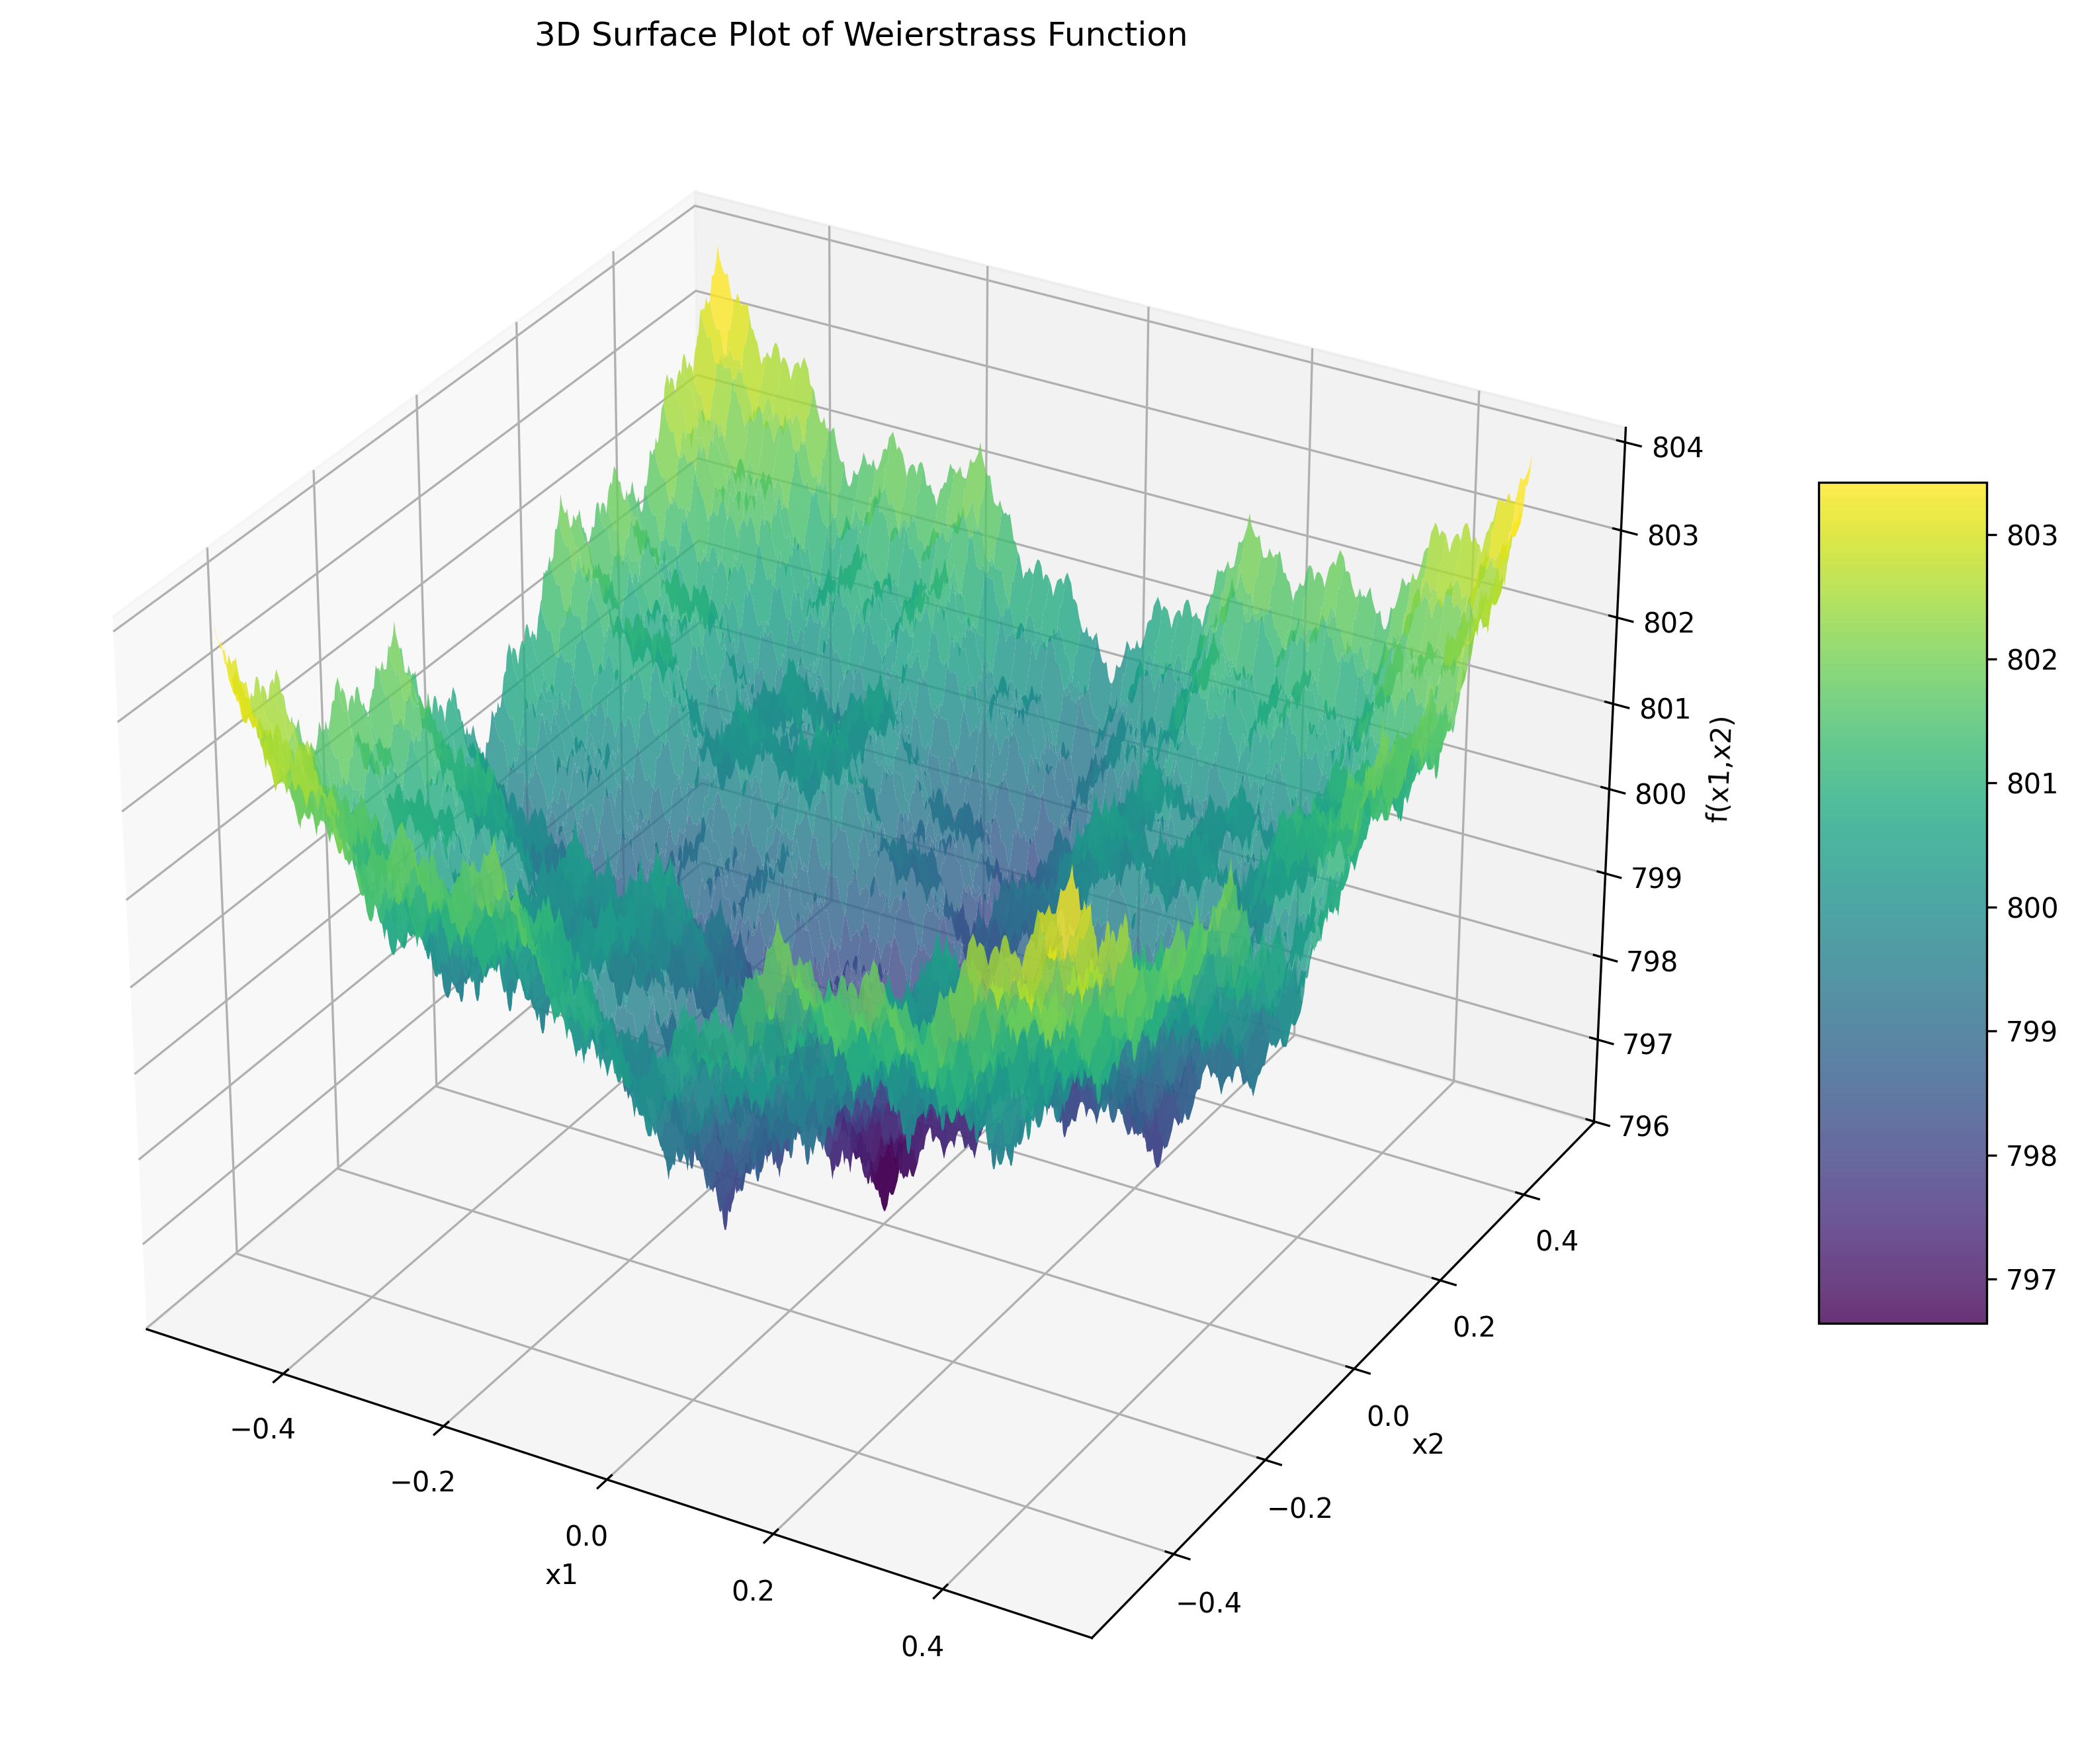
\includegraphics[width=\linewidth]{cec/weierstrass_3d.png}
		\caption{Dimensi 3}
		\label{fig:weierstrass-3d}
	\end{subfigure}
	\caption{Tampilan grafik fungsi Weierstrass pada dimensi dua (\cref{fig:weierstrass-2d}) dan tiga (\cref{fig:weierstrass-3d})}
	\label{fig:weierstrass}
\end{figure}
\begin{equation}
  f_{\text{Weierstrass}}(\mathrm{x})=\sum_{i=1}^{D}\left(\sum_{k=0}^{k\ \text{max}}\left[a^k\cos\left(2\pi b^k\left( z_i+0.5\right)  \right)  \right]  \right)-D\sum_{i=0}^{k \text{max}}\left[ a^k\cos\left(2\pi b^k\cdot0.5 \right) \right]  +f_{\text{bias}}
\end{equation}

\subsubsection*{Zakharov}
\noindent Properti:
\begin{packed_item}
  \item unimodal
  \item convex
  \item non-separable
\end{packed_item}
\begin{figure}[H]
	\centering
	\begin{subfigure}[b]{0.4\textwidth}
		\centering
		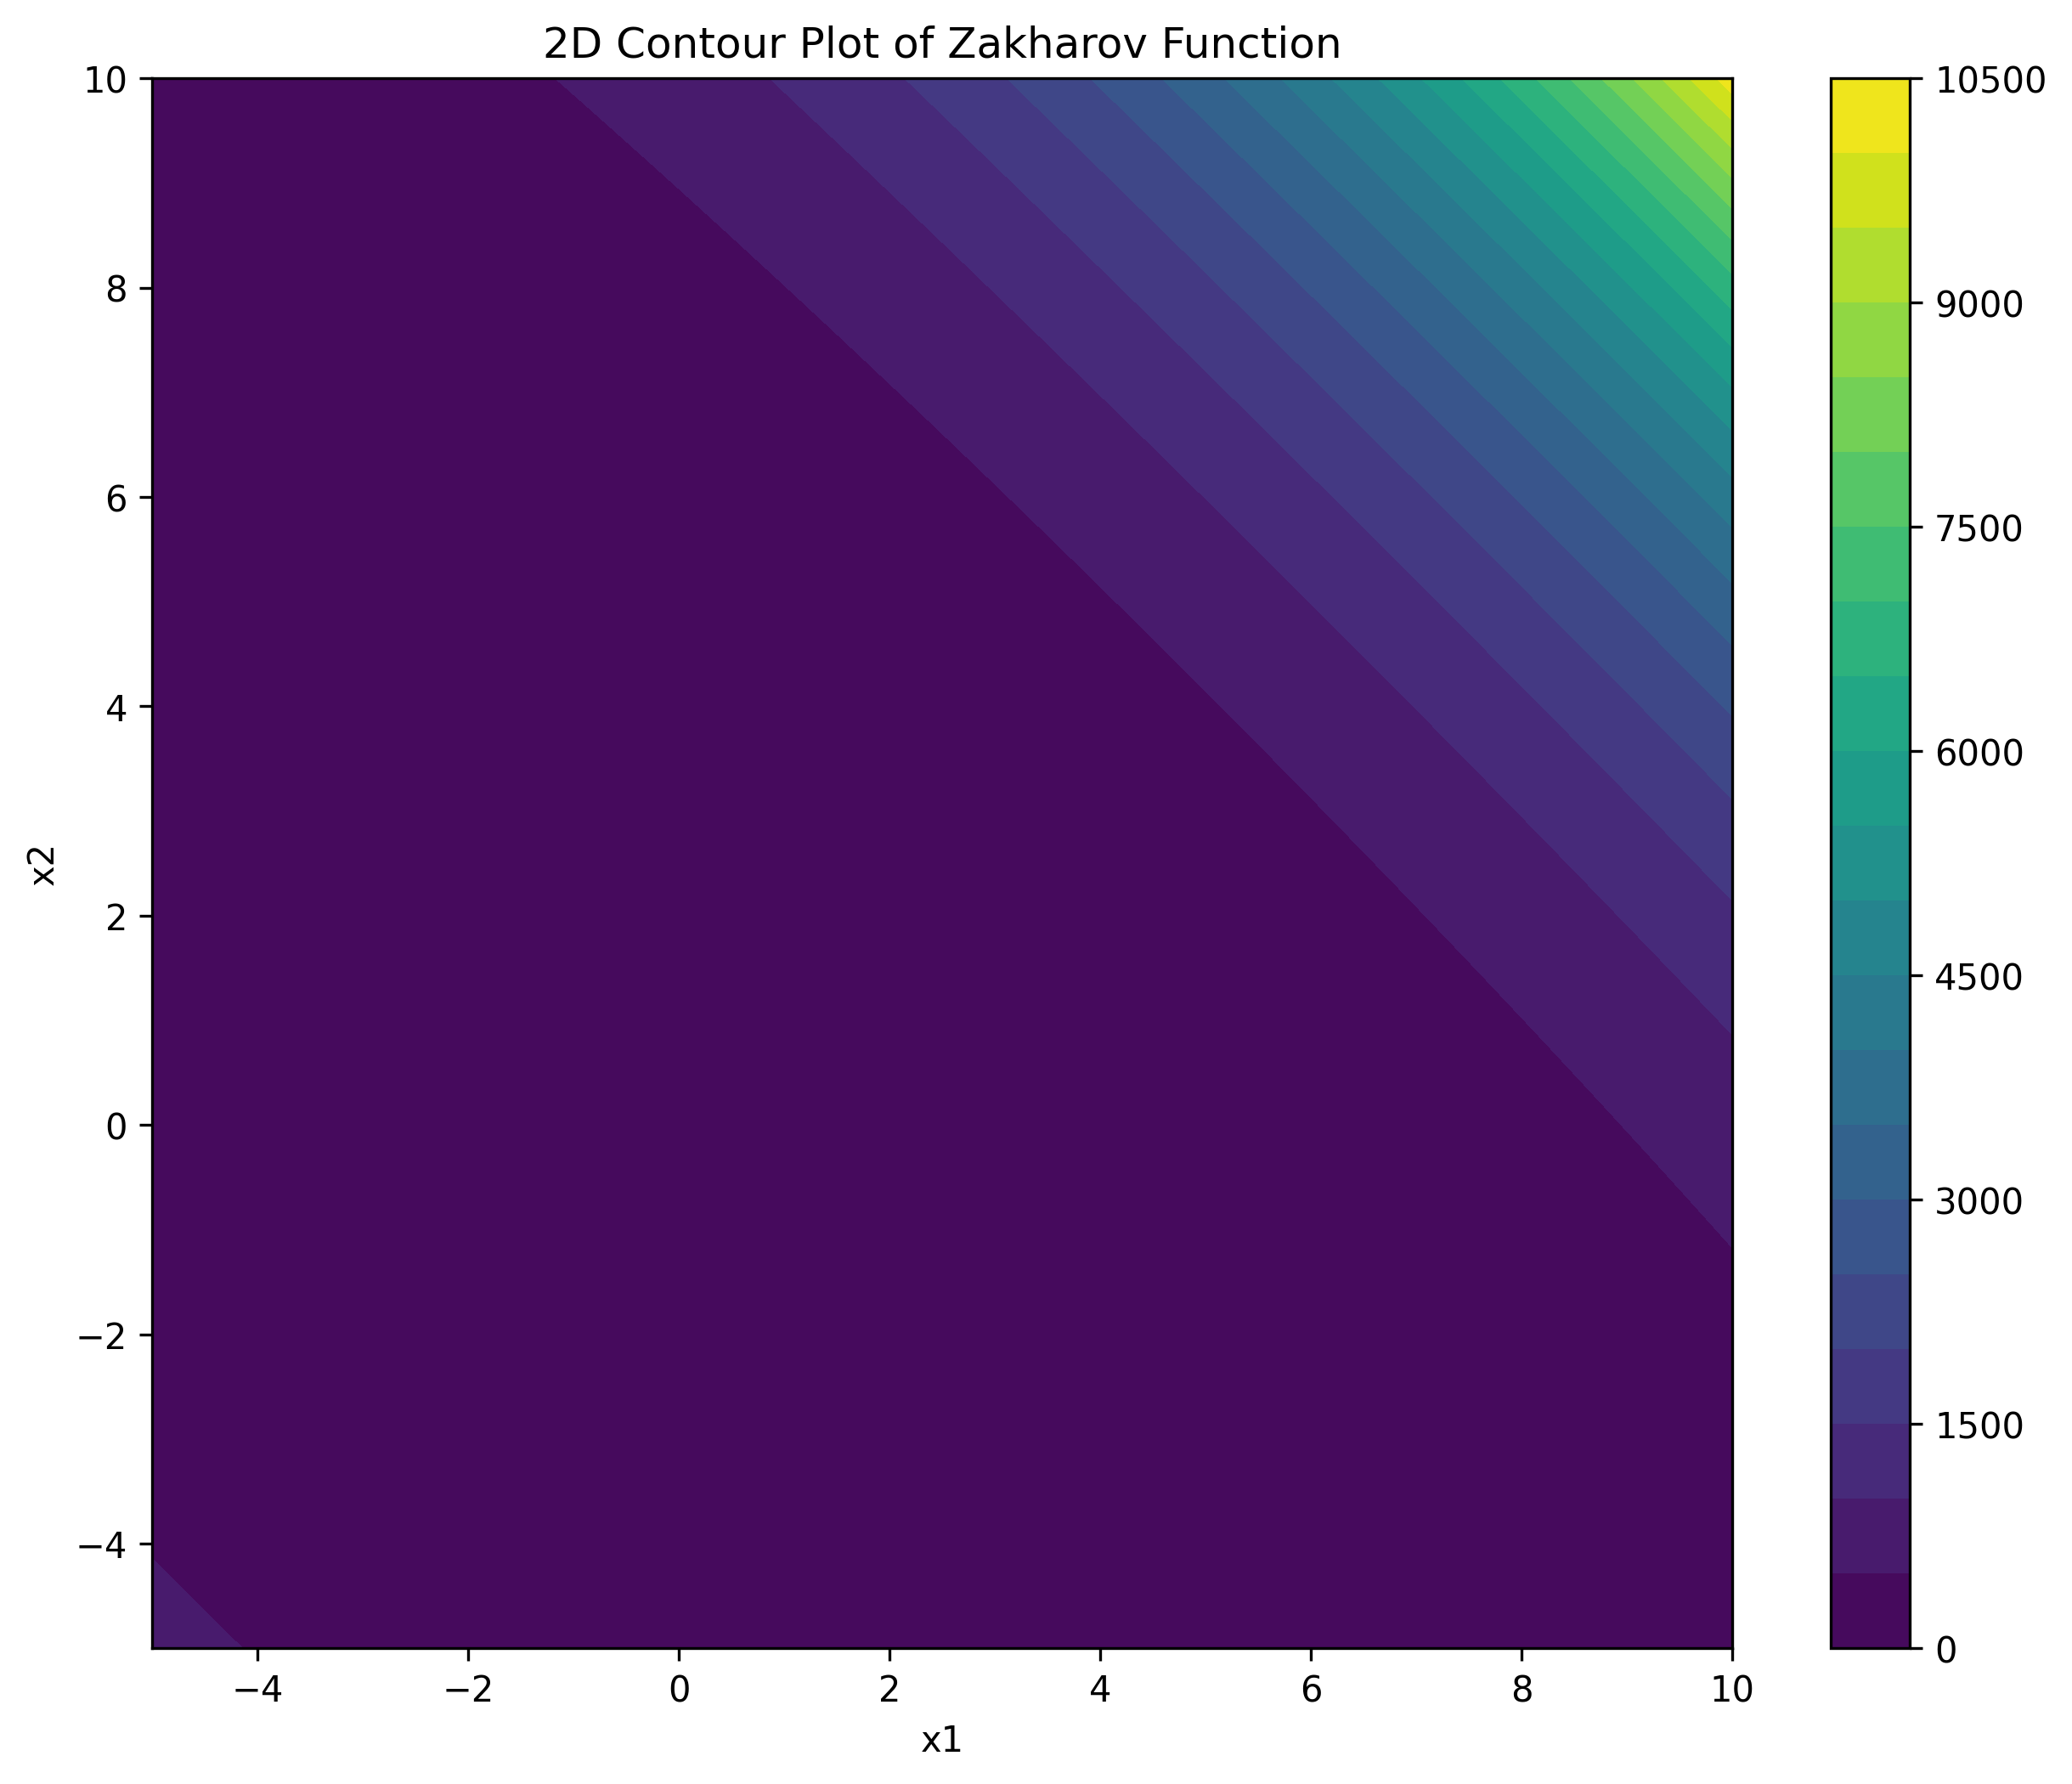
\includegraphics[width=\linewidth]{cec/zakharov_2d.png}
		\caption{Dimensi 2}
		\label{fig:zakharov-2d}
	\end{subfigure}
	\hfill
	\begin{subfigure}[b]{0.4\textwidth}
		\centering
		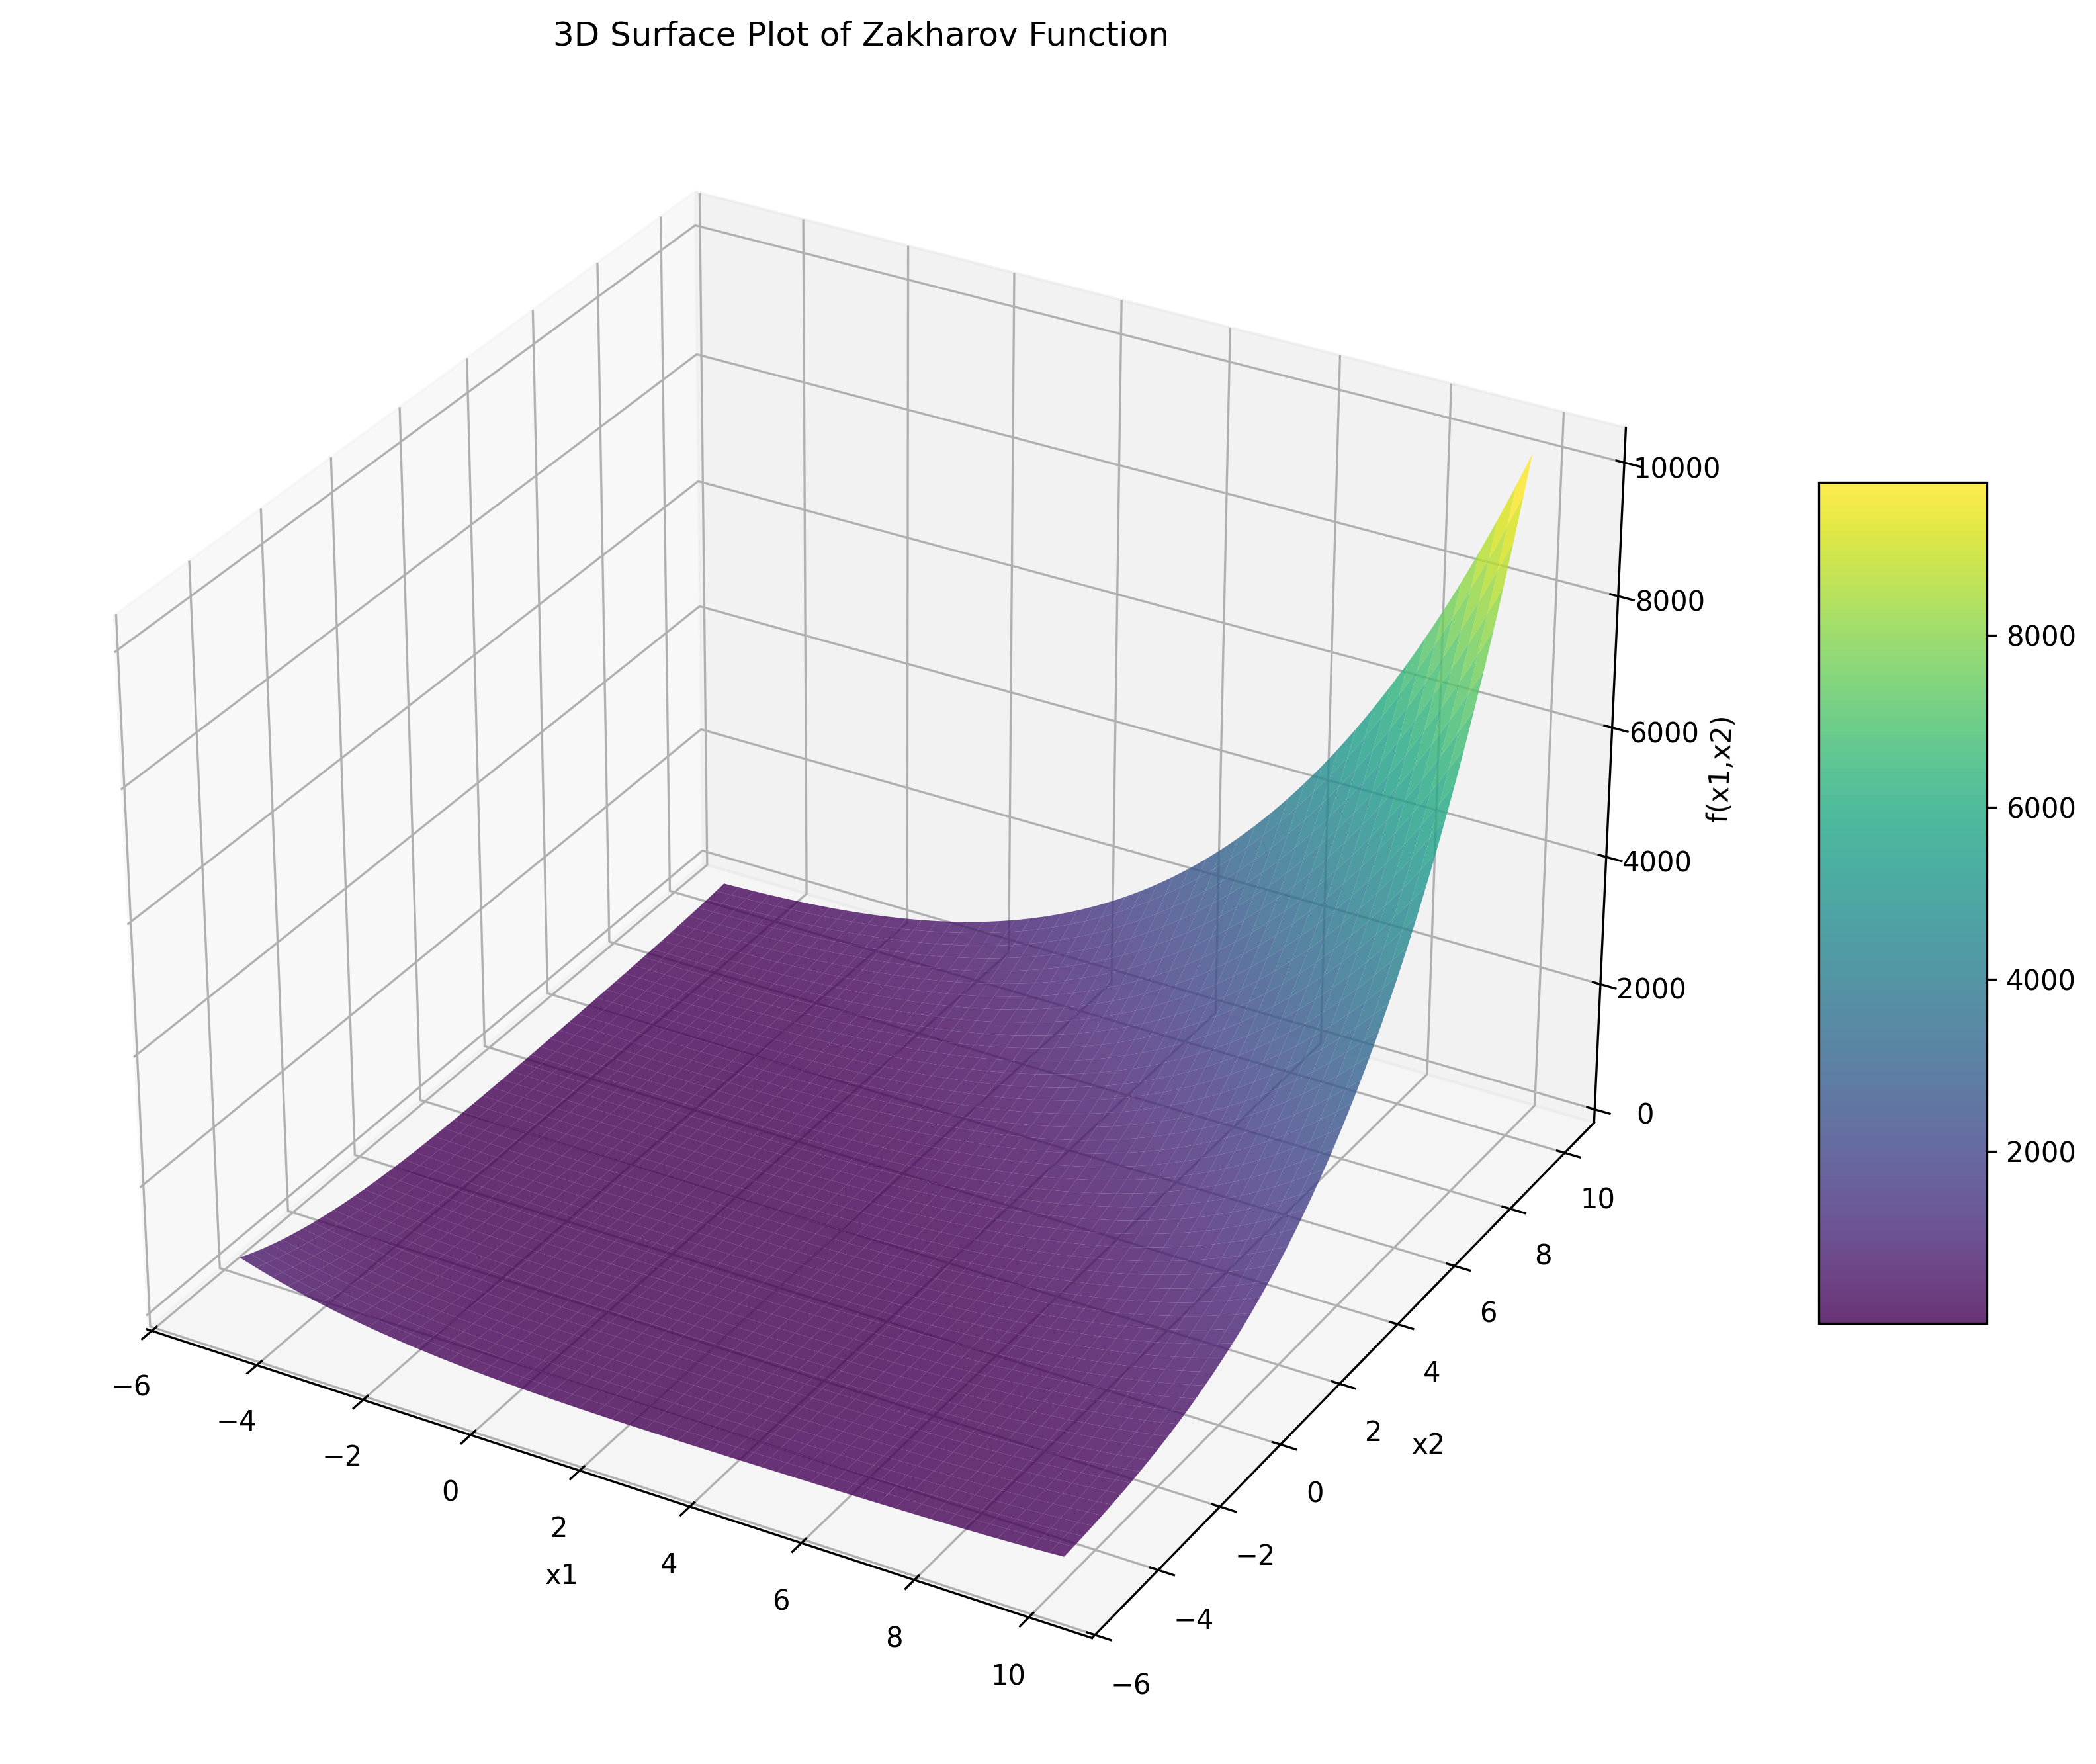
\includegraphics[width=\linewidth]{cec/zakharov_3d.png}
		\caption{Dimensi 3}
		\label{fig:zakharov-3d}
	\end{subfigure}
	\caption{Tampilan grafik fungsi Zakharov pada dimensi dua (\cref{fig:zakharov-2d}) dan tiga (\cref{fig:zakharov-3d})}
	\label{fig:zakharov}
\end{figure}
\begin{equation}
  f_{\text{Zakharov}}(\mathrm{x})=\sum_{i=1}^{D}z_i^2+\left(\sum_{i=1}^{D}0.5z_i \right)^2+\left(\sum_{i=1}^{D}0.5z_i \right)^4+f_{\text{bias}}
\end{equation}

\subsection*{Fungsi COmparing Continuous Optimizers}
Simbol dan definisi yang digunakan dalam fungsi COCO:\\
Lokasi optimal $\mathrm{x}^{\text{opt}}$ dan $f_{\text{opt}} = f(\mathrm{x}^{\text{opt}})$: Semua fungsi memiliki optimum global dalam $[-5, 5]^D$. Sebagian besar fungsi memiliki optimum global dalam $[-4, 4]^D$, dan untuk banyak di antaranya, $\mathrm{x}^{\text{opt}}$ diambil secara seragam dari kompak ini.\\
\noindent$\otimes$ menunjukkan perkalian per elemen antara dua vektor berdimensi $D$, $\otimes:R^D\times R^D\to R^D, (\mathrm{x},\mathrm{y})\mapsto \text{diag}(\mathrm{x})\times\mathrm{y}=(x_i\times y_i)_{i=1},\ldots,D$\\
$||\cdot||$ menunjukkan Euclidean norm, $||\mathrm{x}||^2=\sum_{i}x^2_i$\\
$\left[\cdot\right]$ menunjukkan nilai bilangan bulat terdekat\\
$\textbf{0}=(0,\ldots,0)^{\mathrm{T}}$ vektor yang semuanya bernilai 0\\
$\textbf{1}=(1,\ldots,1)^{\mathrm{T}}$ vektor yang semuanya bernilai 1\\
$\Lambda^{\alpha}$ adalah sebuah matriks diagonal berdimensi $D$ dengan elemen diagonal ke-$i$ sebagai $\lambda_{ii}=\alpha^{\frac{1}{2}\frac{i-1}{D-1}}$, untuk $i=1,\ldots,D$\\
$f_{\text{pen}}:\mathcal{R}^D\to \mathcal{R}, \mathrm{x}\mapsto\sum_{i=1}^{D}\max(0,\left|x_i\right|-5)^2$\\
$\textbf{1}\pm$ sebuah vektor berdimensi $D$ dengan entri bernilai $-1$ atau $1$ yang diambil secara independen dengan peluang yang sama.\\
$\bf{Q, R}$ matriks ortogonal (matriks rotasi). Untuk satu fungsi dalam satu dimensi, realisasi yang berbeda untuk $Q$ dan $R$ masing-masing digunakan untuk setiap perwujudan fungsi tersebut. Ortogonal matriks dihasilkan dari entri berdistribusi normal standar melalui ortonormalisasi gram-schmidt. Kolom dan baris pada matriks ortogonal membentuk basis ortonormal.\\
$\bf{R}$ lihat $\bf{Q}$\\
$T_{\text{asy}}^{\beta}:\mathcal{R}^D\to \mathcal{R}^D,x_i\mapsto \begin{cases}
  x_i^{1+\beta\frac{i-1}{D-1}\sqrt{x_i}} & \text{jika } x_i > 0\\
  x_i & \text{selain itu}
\end{cases}, \text{untuk } i=1,\ldots,D$.\\
$T_{\text{osz}}:\mathcal{R}^n\to \mathcal{R}^n$, untuk sembarang bilangan bulat positif $n(n=1 \text{ dan } n=D \text{ yang digunakan berikut ini})$ peta kan \textit{element-wise}\\
\vspace*{-2.5em}
\[x\mapsto \sign(x) \exp(\hat{x}+0.049(\sin(c_1\hat{x})+\sin(c_2\hat{x})))\]
dengan $\hat{x}=\begin{cases}
  \log(\left|x\right|) & \text{jika } x > 0\\
  0 & \text{selain itu}
\end{cases}, \sign(x)=\begin{cases}
  -1 & \text{jika } x < 0\\
  0 & \text{jika } x = 0\\
  1 & \text{selain itu}
\end{cases},c_1=\begin{cases}
  10 & \text{jika } x > 0\\
  5.5 & \text{selain itu}
\end{cases}\text{ dan}\\ c_2=\begin{cases}
  7.9 & \text{jika } x > 0\\
  3.1 & \text{selain itu}
\end{cases}$.\\
$\mathrm{x}^{\text{opt}}$ vektor solusi optimal, sehingga $f(\mathrm{x}^{\text{opt}})$ adalah minimal.

\subsubsection*{Attractive sector}
\noindent Properti:
fungsi dengan asimetris tingkat tinggi, di mana hanya terdapat satu \textit{hyperplane} bervolume sekitar $\frac{1}{2}^D$ yang memberikan nilai fungsi kecil.
\begin{packed_item}
  \item unimodal
\end{packed_item}
\begin{figure}[H]
	\centering
	\begin{subfigure}[b]{0.4\textwidth}
		\centering
		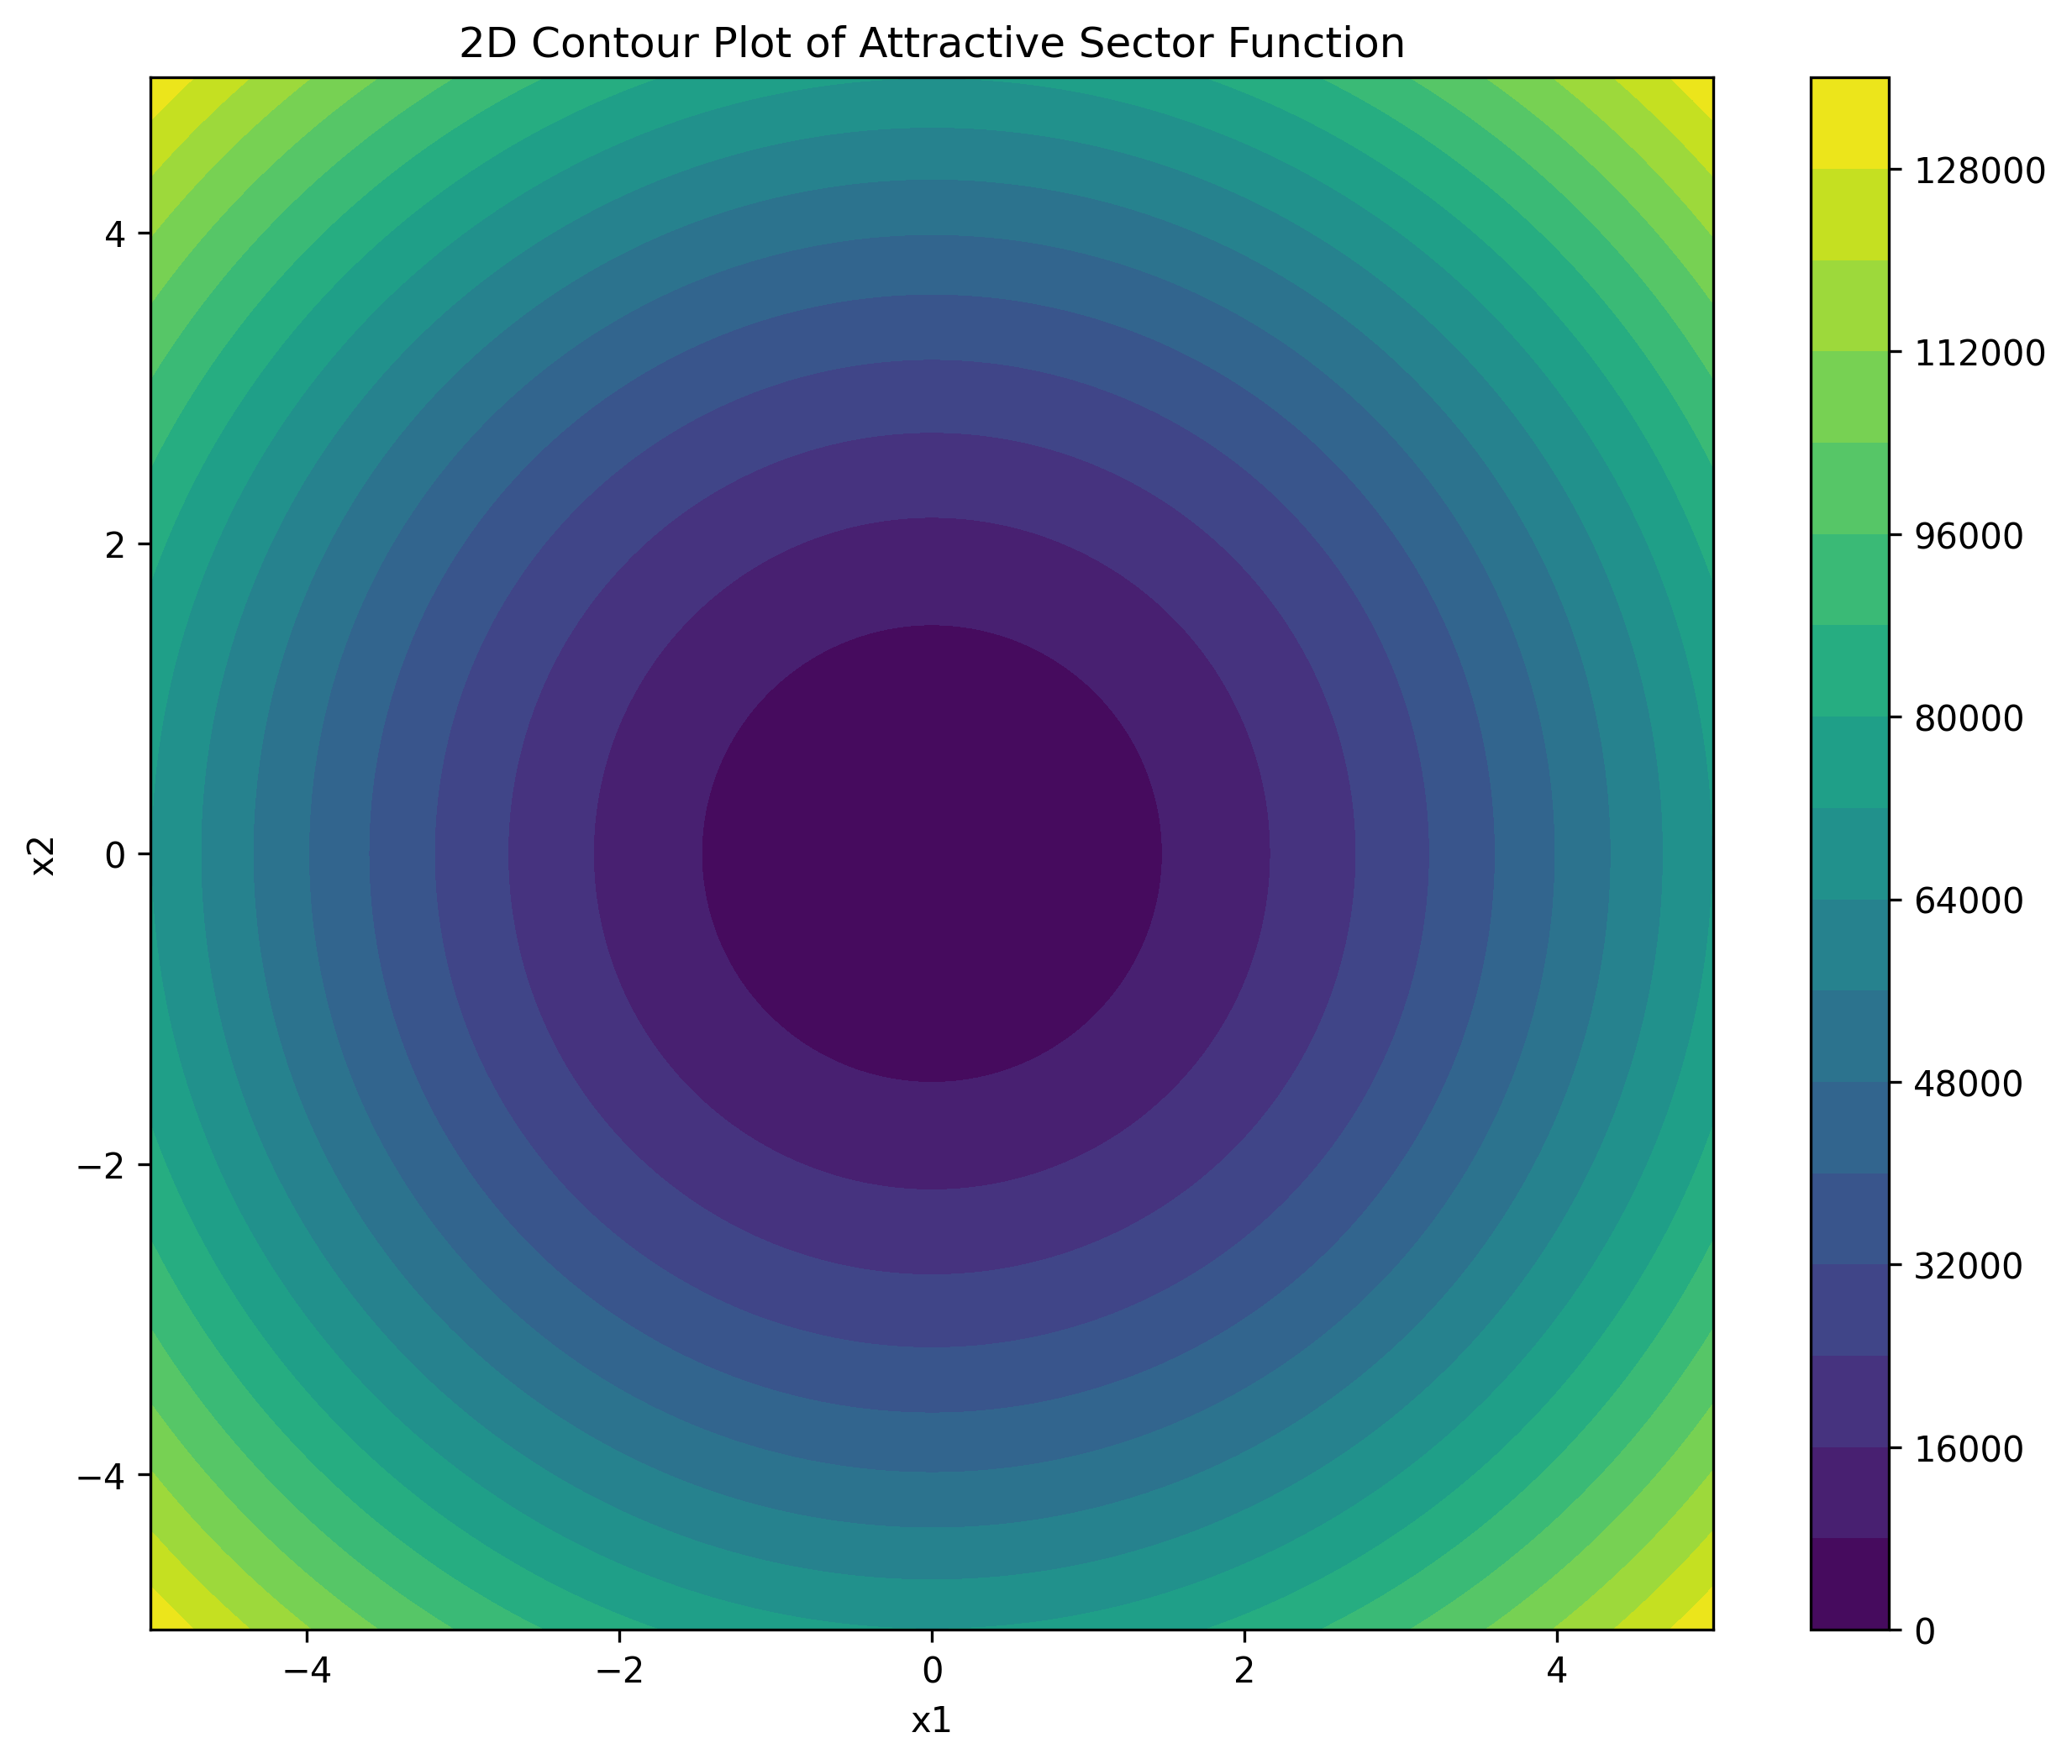
\includegraphics[width=\linewidth]{coco/attr_2d.png}
		\caption{Dimensi 2}
		\label{fig:attr-2d}
	\end{subfigure}
	\hfill
	\begin{subfigure}[b]{0.4\textwidth}
		\centering
		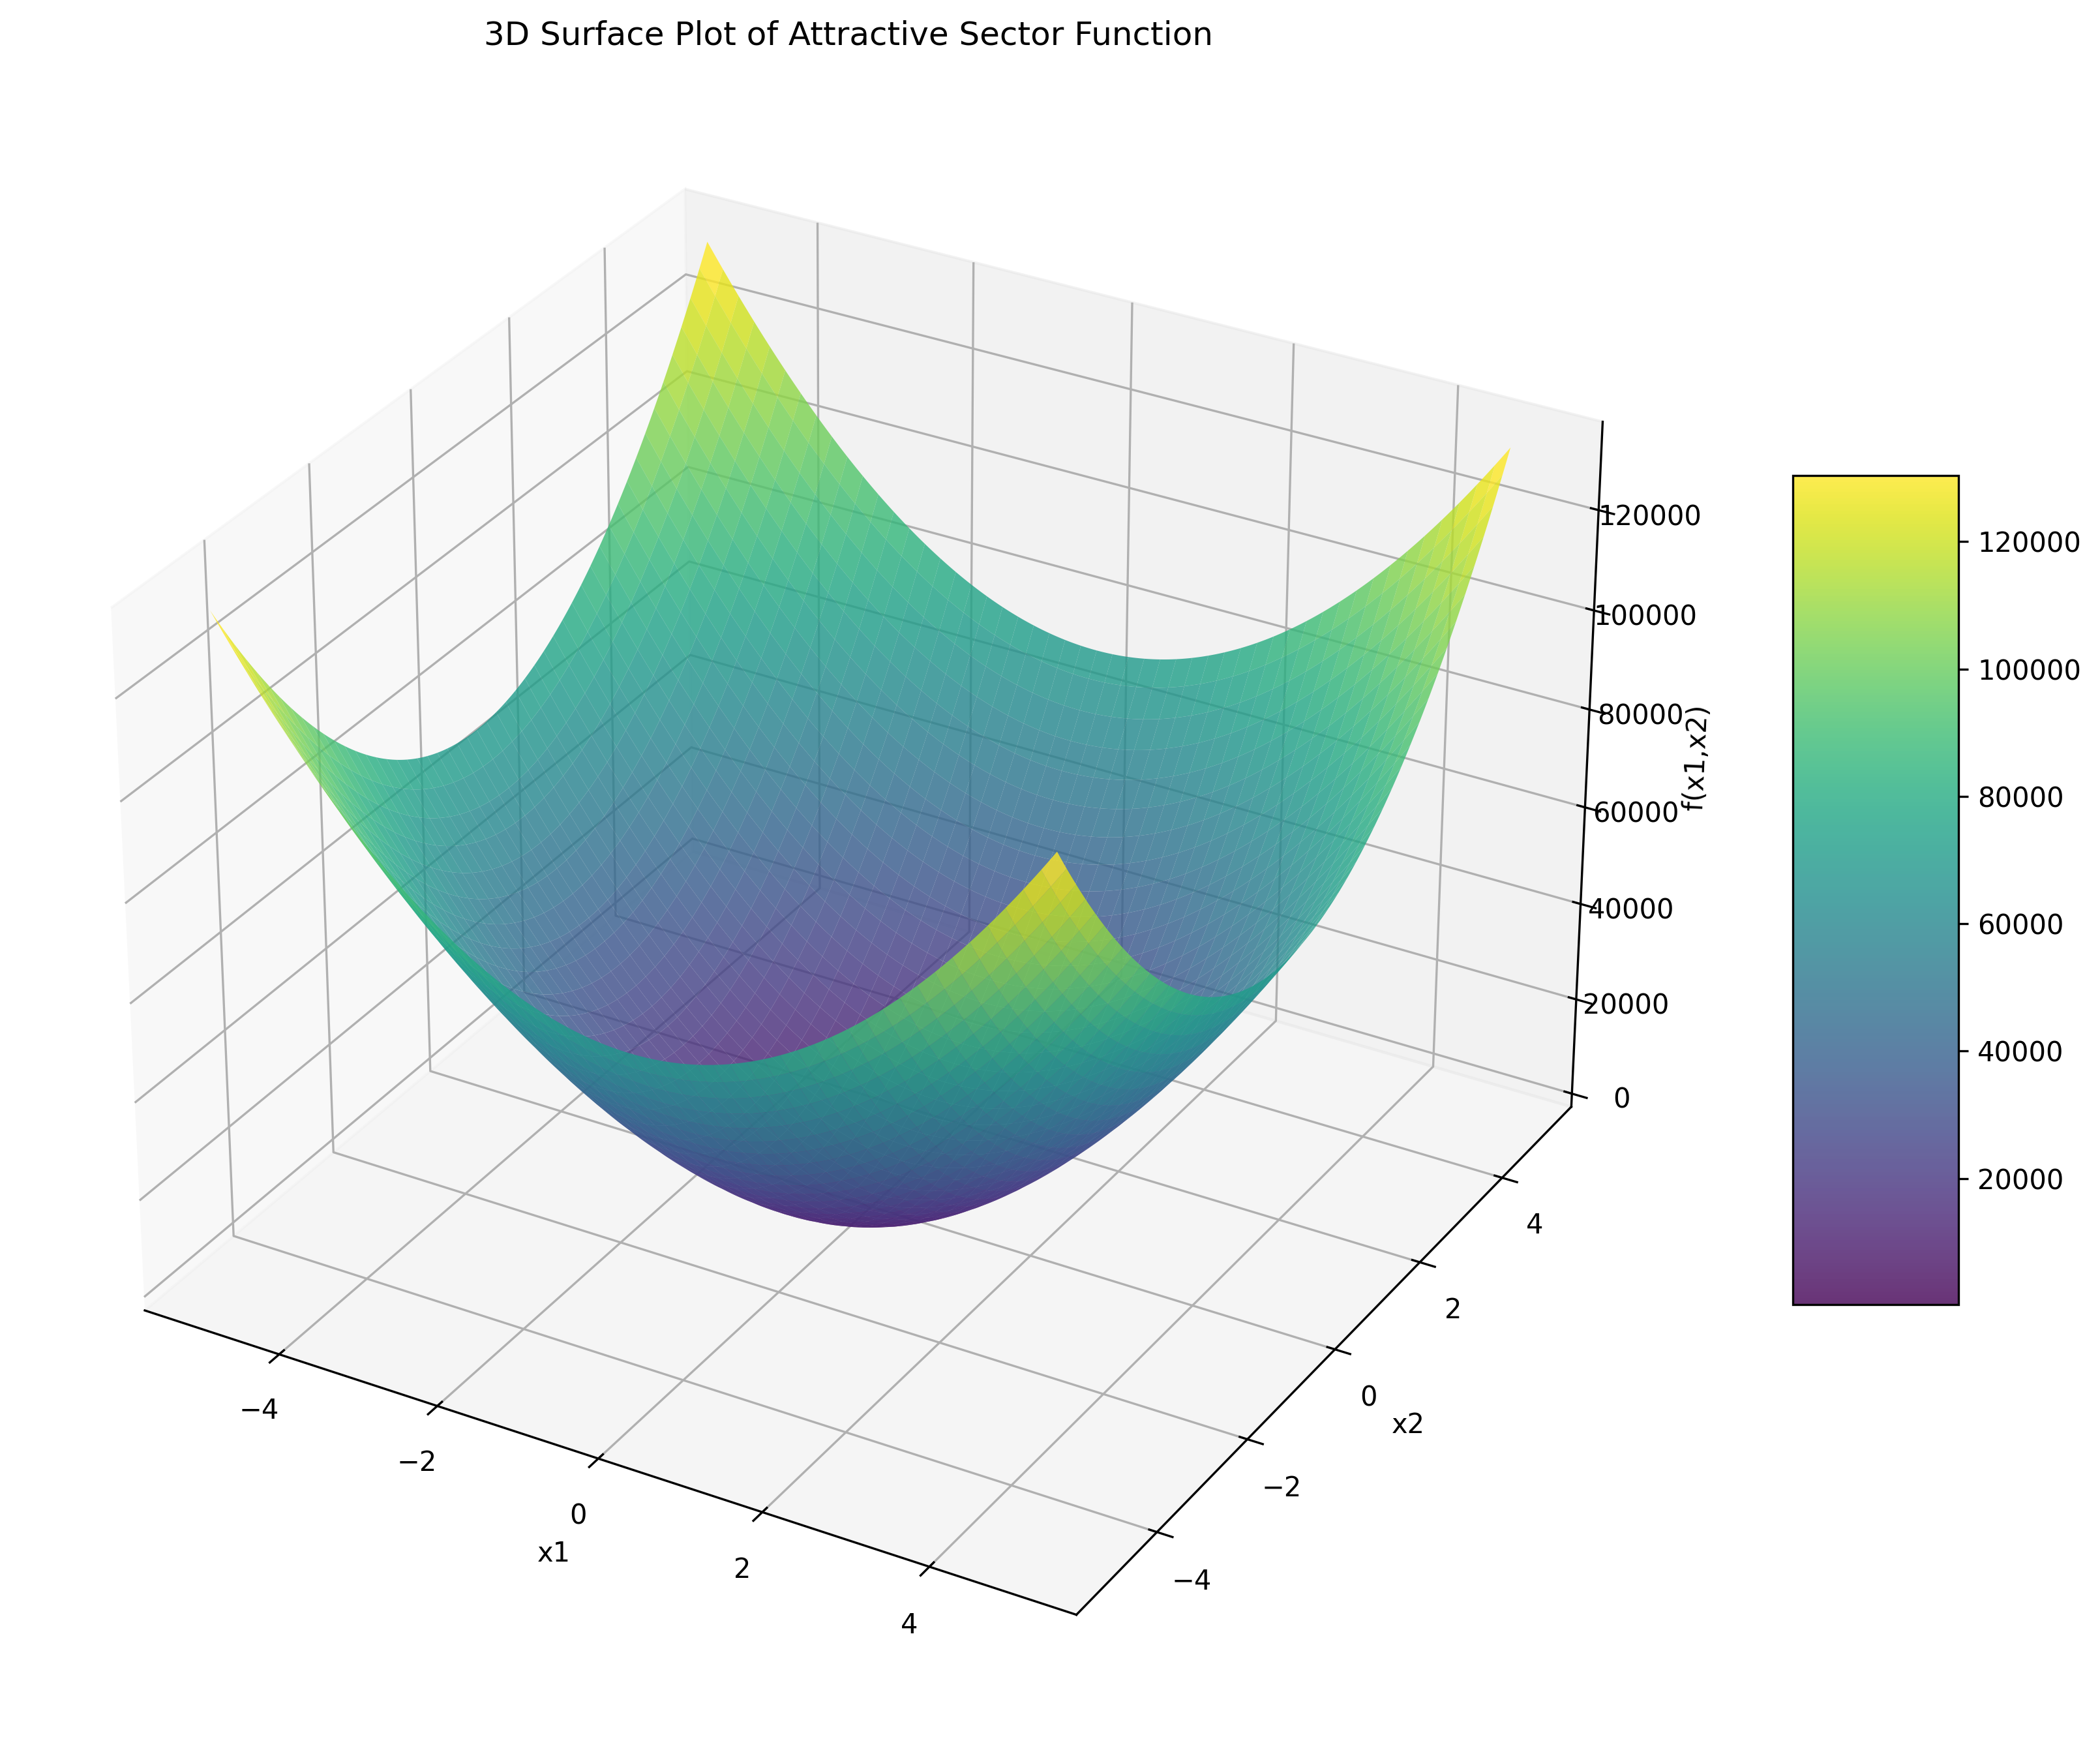
\includegraphics[width=\linewidth]{coco/attr_3d.png}
		\caption{Dimensi 3}
		\label{fig:attr-3d}
	\end{subfigure}
	\caption{Tampilan grafik fungsi Attractive sector pada dimensi dua (\cref{fig:attr-2d}) dan tiga (\cref{fig:attr-3d}) tanpa transformasi input}
	\label{fig:atrr}
\end{figure}
\begin{equation}
  f_{\text{Attractive sector}}(\mathrm{x})=\mathrm{T}_{\text{osz}}(\sum_{i=1}^{D}(s_iz_i)^2)^{0.9}+f_{\text{opt}}
\end{equation}
\begin{packed_item}
    \item $\mathrm{z}=Q\Lambda^{10}R(\mathrm{x}-\mathrm{x}^{\text{opt}})$
    \item $s_i\begin{cases}
      10^2 & \text{jika }z_i\times x_i^{\text{opt}}>0\\
      1 & \text{selain itu}
    \end{cases}$
\end{packed_item}

\subsubsection*{Bent cigar}
\noindent Properti:
\begin{packed_item}
  \item unimodal
  \item struktur ketergantungan \textit{tri-band}, pada dimensi yang lebih tinggi fungsi ini memiliki optimal lokal dengan volume daya tarik sebesar 25\%
\end{packed_item}
\begin{figure}[H]
	\centering
	\begin{subfigure}[b]{0.4\textwidth}
		\centering
		\includegraphics[width=\linewidth]{coco/bent_cigar_2d.png}
		\caption{Dimensi 2}
		\label{fig:bent-cigar-coco-2d}
	\end{subfigure}
	\hfill
	\begin{subfigure}[b]{0.4\textwidth}
		\centering
		\includegraphics[width=\linewidth]{coco/bent_cigar_3d.png}
		\caption{Dimensi 3}
		\label{fig:bent-cigar-coco-3d}
	\end{subfigure}
	\caption{Tampilan grafik fungsi Bent cigar pada dimensi dua (\cref{fig:bent-cigar-coco-2d}) dan tiga (\cref{fig:bent-cigar-coco-3d}) tanpa transformasi input}
	\label{fig:bent_cigar_coco}
\end{figure}
\begin{equation}
  f_{\text{Bent cigar}}(\mathrm{x})=\sum_{i=1}^{D-1}(100(z_i^2-z_{i+1})^2+(z_i-1)^2)+f_{\text{opt}}
\end{equation}
\begin{packed_item}
    \item $\mathrm{z}=\max(1,\frac{\sqrt{D}}{8})(\mathrm{x}-\mathrm{x}^{\text{opt}})+1$
    \item $\mathrm{z}^{\text{opt}}=1$
\end{packed_item}

\subsubsection*{Büche-Rastrigin}
\noindent Properti:
\begin{packed_item}
  \item sekitar $10^D$ optimum lokal, faktor pengkodisian sekitar 10, faktor \textit{skew} sekitar 10 di ruang ruang-$x$ dan 100 di ruang-$f$ 
\end{packed_item}
\begin{figure}[H]
	\centering
	\begin{subfigure}[b]{0.4\textwidth}
		\centering
		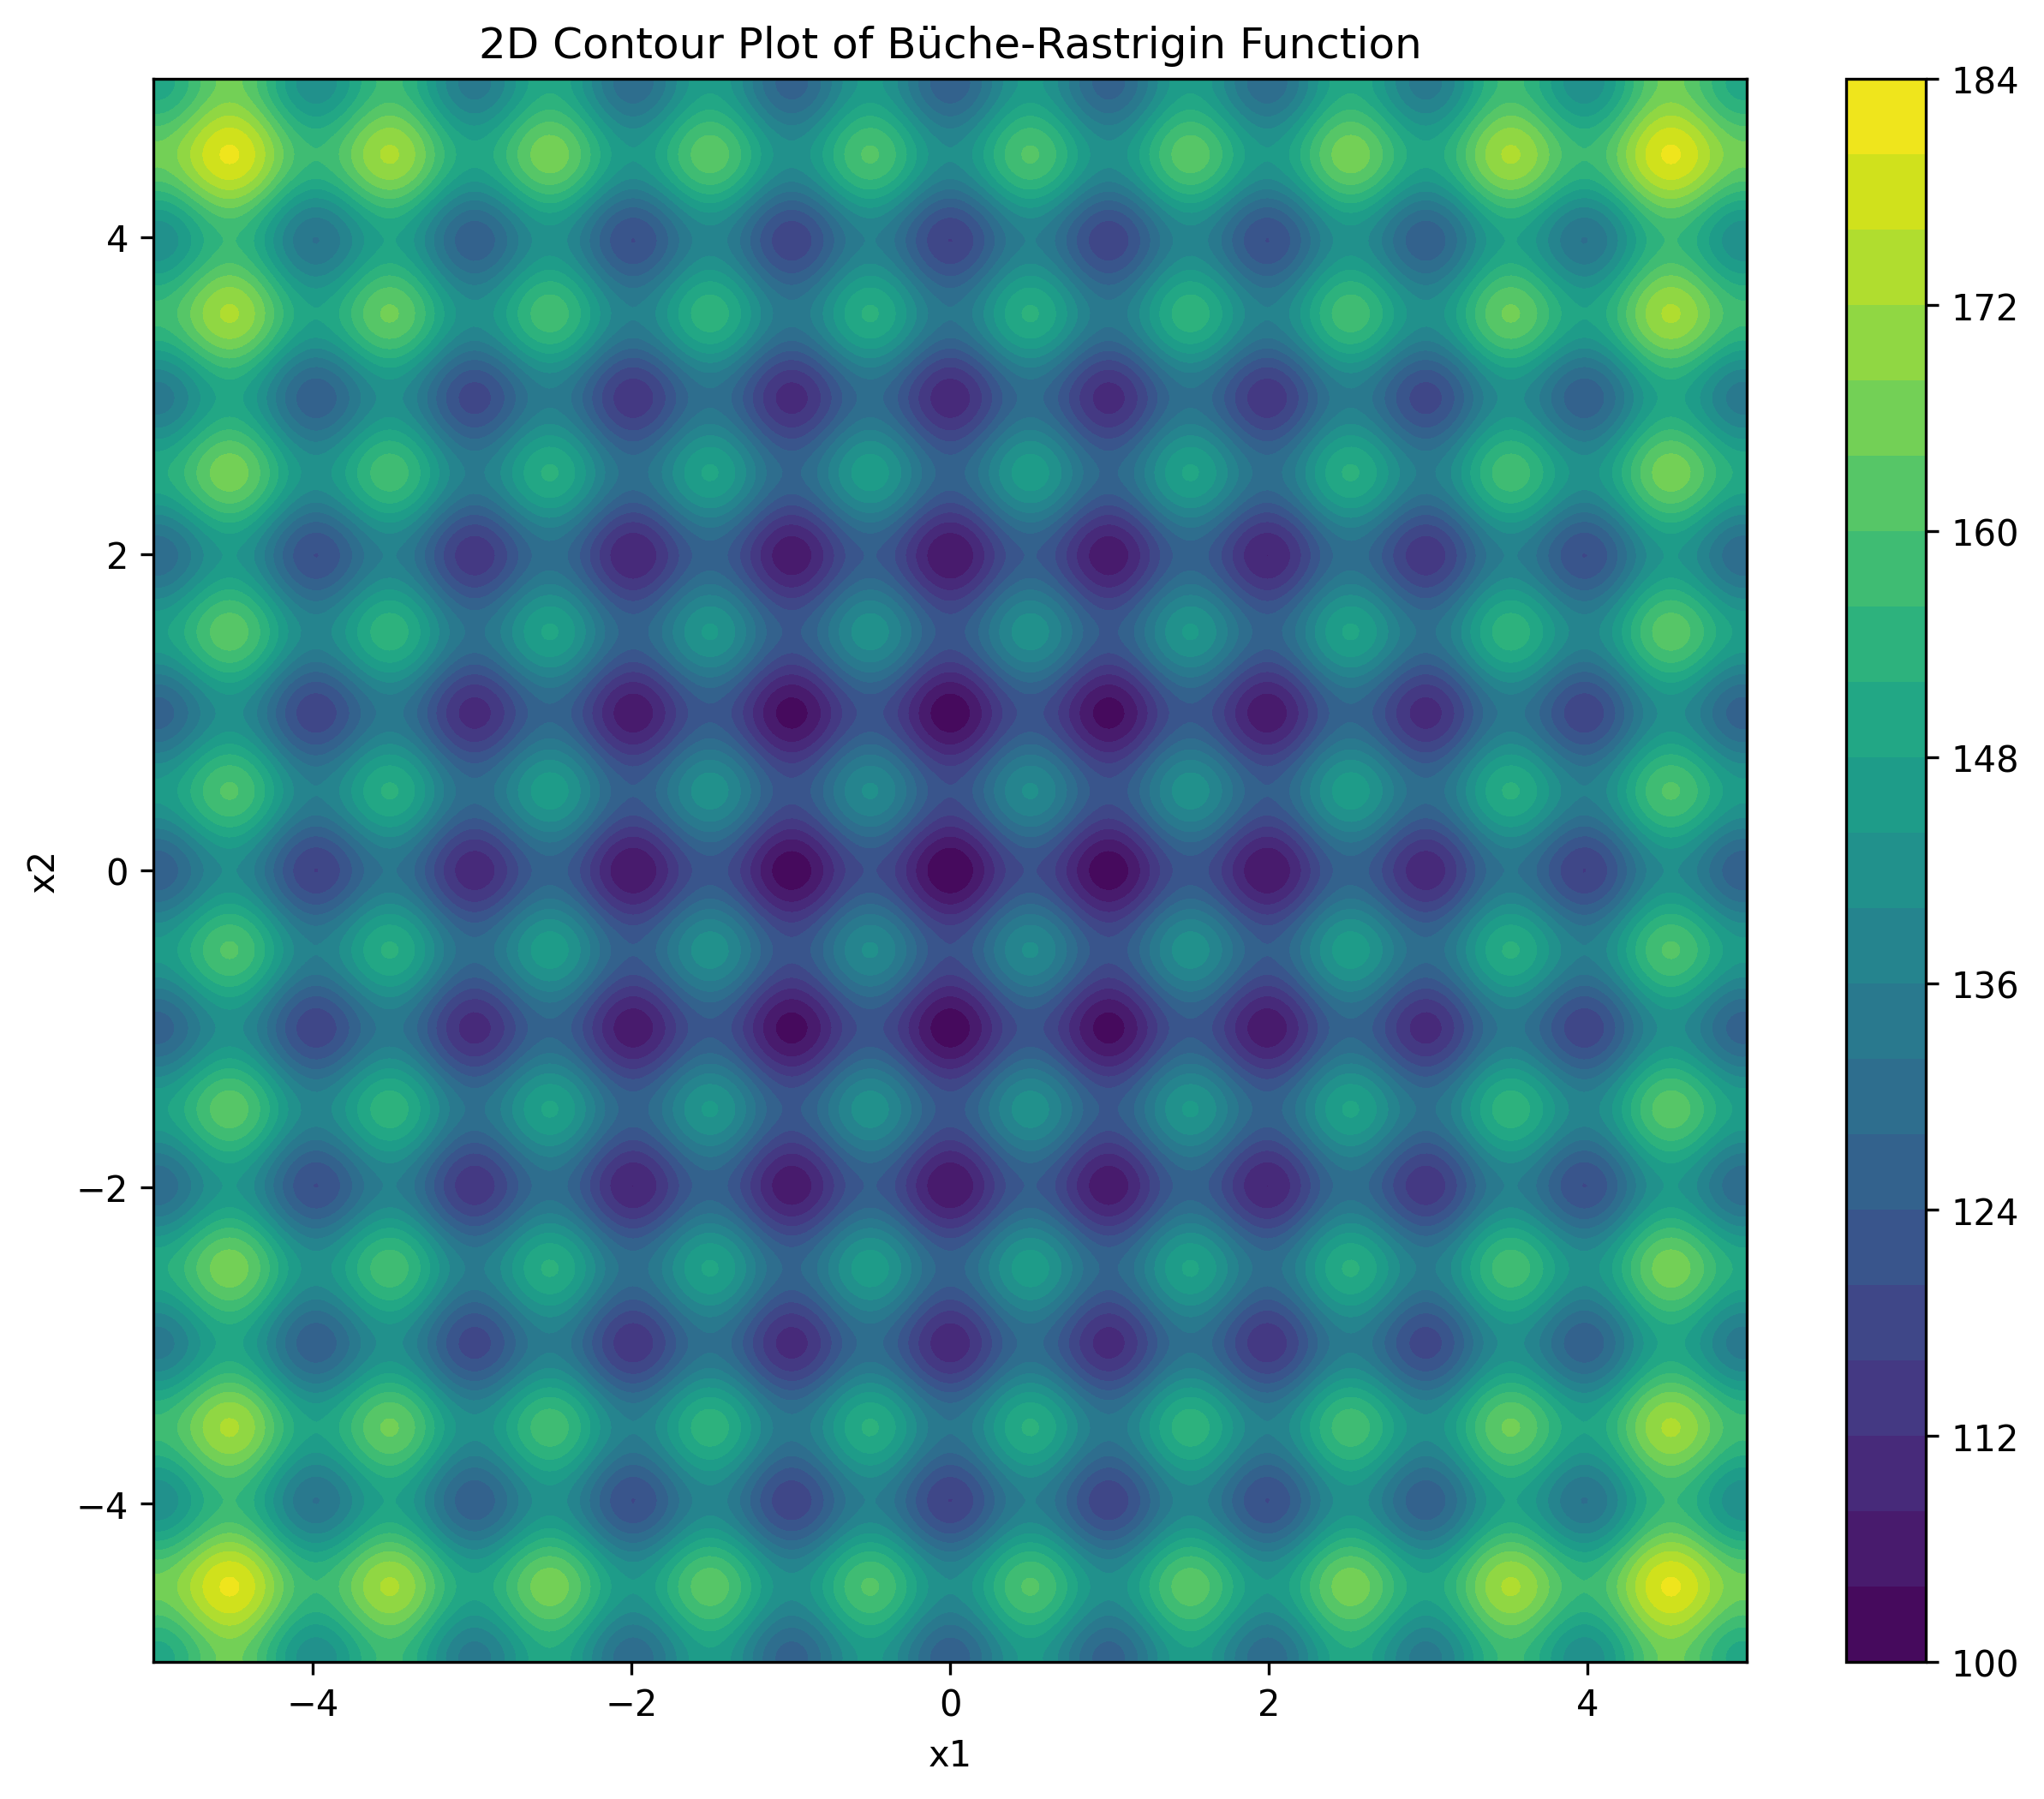
\includegraphics[width=\linewidth]{coco/buche_rastrigin_2d.png}
		\caption{Dimensi 2}
		\label{fig:buche-rastrigin-2d}
	\end{subfigure}
	\hfill
	\begin{subfigure}[b]{0.4\textwidth}
		\centering
		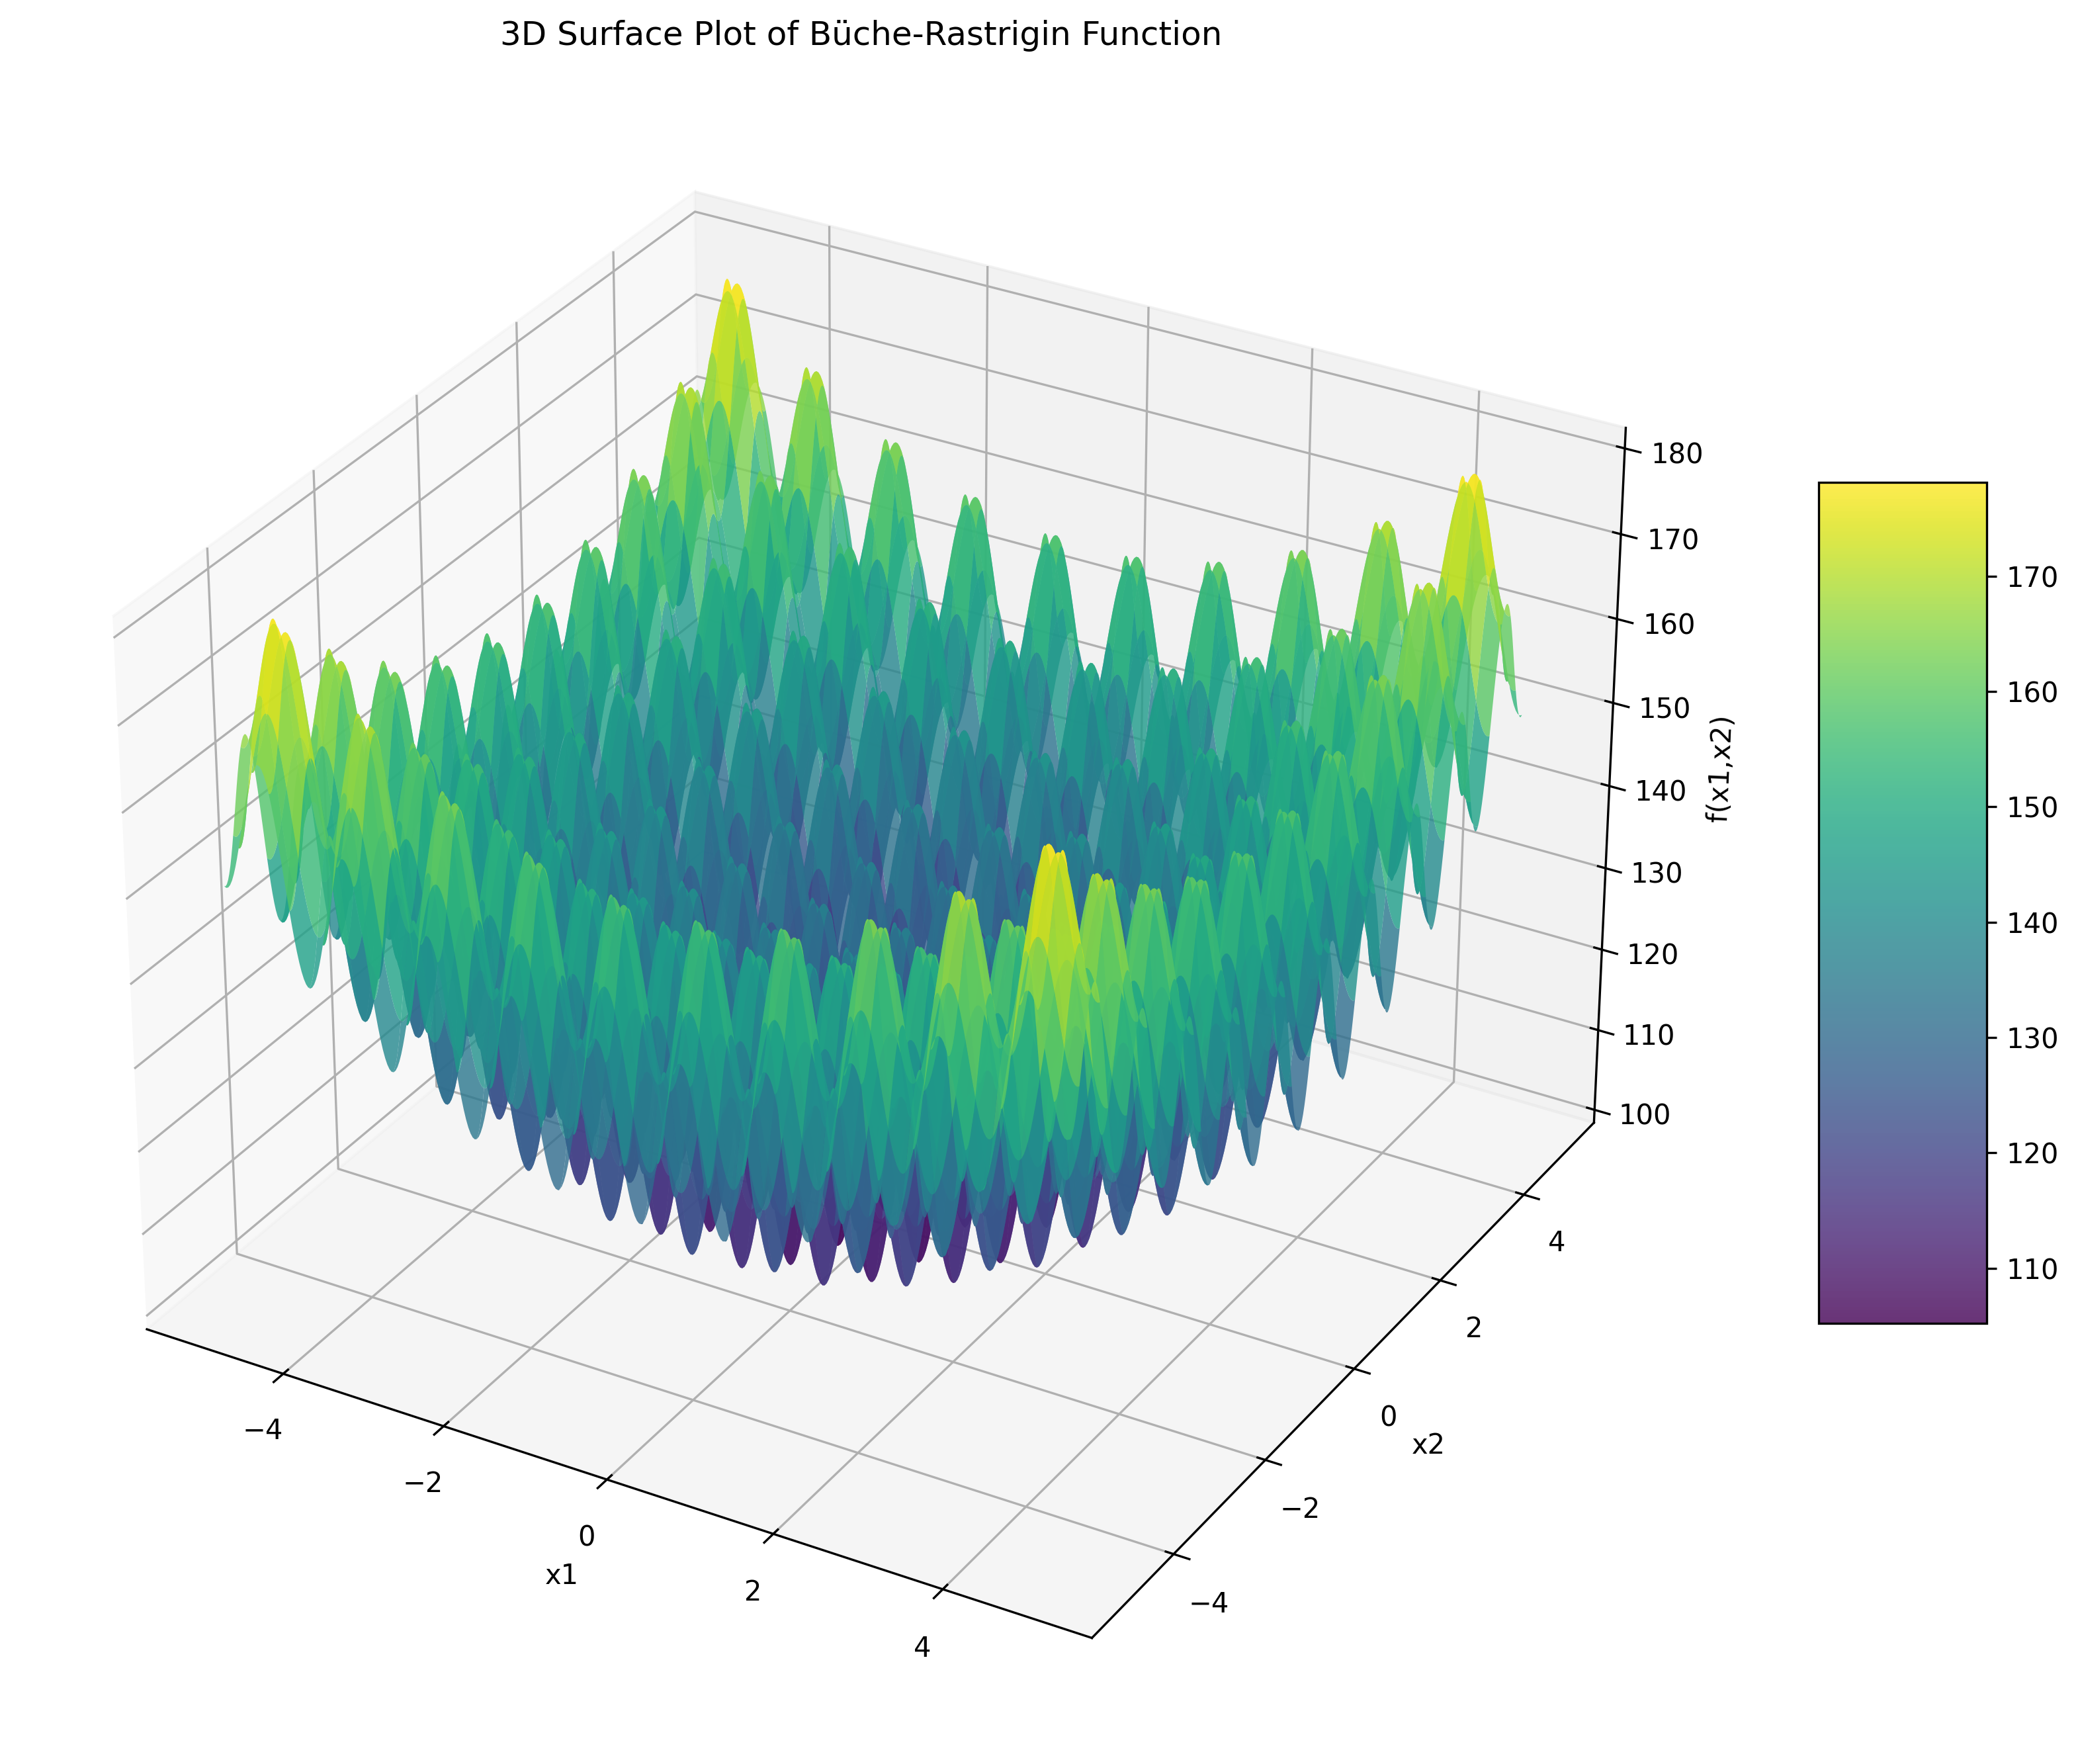
\includegraphics[width=\linewidth]{coco/buche_rastrigin_3d.png}
		\caption{Dimensi 3}
		\label{fig:buche-rastrigin-3d}
	\end{subfigure}
	\caption{Tampilan grafik fungsi Büche-Rastrigin pada dimensi dua (\cref{fig:buche-rastrigin-2d}) dan tiga (\cref{fig:buche-rastrigin-3d}) tanpa transformasi input}
	\label{fig:buche_rastrigin}
\end{figure}
\begin{equation}
  f_{\text{Büche-Rastrigin}}(\mathrm{x})=10(D-\sum_{i=1}^{D}\cos(2\pi z_i))+\sum_{i=1}^{D}z_i^2+100f_{\text{pen}}(\mathrm{x})+f_{\text{opt}}
\end{equation}
\begin{packed_item}
    \item $z_i=s_iT_{\text{osz}}(\mathrm{x}-\mathrm{x}^{\text{opt}})$ untuk $i=1,\ldots,D$
    \item $s_i=\begin{cases}
      10\times 10^{\frac{1}{2}\frac{i-1}{D-1}} & \text{jika }z_i > 0 \text{ dan } i=1,3,5,\ldots\\
      10^{\frac{1}{2}\frac{i-1}{D-1}} & \text{selain itu}
    \end{cases} \text{ untuk }i=1,\ldots,D$
\end{packed_item}

\subsubsection*{Composite griewank-rosenbrock function F8F2}
\noindent Properti:
menyerupai fungsi rosenbrock dengan dalam sifat yang sangat multimodal
\begin{figure}[H]
	\centering
	\begin{subfigure}[b]{0.4\textwidth}
		\centering
		\includegraphics[width=\linewidth]{coco/griewank_rosenbrock_2d.png}
		\caption{Dimensi 2}
		\label{fig:griewank-rosenbrock-2d}
	\end{subfigure}
	\hfill
	\begin{subfigure}[b]{0.4\textwidth}
		\centering
		\includegraphics[width=\linewidth]{coco/griewank_rosenbrock_3d.png}
		\caption{Dimensi 3}
		\label{fig:griewank-rosenbrock-3d}
	\end{subfigure}
	\caption{Tampilan grafik fungsi Composite griewank-rosenbrock function F8F2 pada dimensi dua (\cref{fig:griewank-rosenbrock-2d}) dan tiga (\cref{fig:griewank-rosenbrock-3d}) tanpa transformasi input}
	\label{fig:griewank_rosenbrock}
\end{figure}
\begin{equation}
  f_{\text{Büche-Rastrigin}}(\mathrm{x})=\frac{10}{D-1}\sum_{i=1}^{D-1}(\frac{s_i}{4000}-\cos(s_i))+10+f_{\text{opt}}
\end{equation}
\begin{packed_item}
    \item $\mathrm{z}=\max(1,\frac{\sqrt{D}}{8})R\mathrm{x}+0.5$
    \item $s_i=100(z_i^2-z_{i+1})^2+(z_i-1)^2$ untuk $i=1,\ldots,D$
    \item $\mathrm{z}^{\text{opt}}=1$
\end{packed_item}

\subsubsection*{Different power}
\noindent Properti:
karena perbedaan exponen, sensitivitas variabel $z_i$ menjadi semakin berbeda ketika mendekati titik optimum.
\begin{figure}[H]
	\centering
	\begin{subfigure}[b]{0.4\textwidth}
		\centering
		\includegraphics[width=\linewidth]{coco/different_power_2d.png}
		\caption{Dimensi 2}
		\label{fig:dp_2d}
	\end{subfigure}
	\hfill
	\begin{subfigure}[b]{0.4\textwidth}
		\centering
		\includegraphics[width=\linewidth]{coco/different_power_3d.png}
		\caption{Dimensi 3}
		\label{fig:dp_3d}
	\end{subfigure}
	\caption{Tampilan grafik fungsi Different power pada dimensi dua (\cref{fig:dp_2d}) dan tiga (\cref{fig:dp_3d}) tanpa transformasi input}
	\label{fig:different_power_coco}
\end{figure}
\begin{equation}
  f_{\text{Different power}}(\mathrm{x})=\sqrt{\sum_{i=1}^{D}|z_i|^{2+4\frac{i-1}{D-1}}}+f_{\text{opt}}
\end{equation}
\begin{packed_item}
    \item $\mathrm{z}=R(\mathrm{x}-\mathrm{x}^{\text{opt}})$
\end{packed_item}

\subsubsection*{Discus}
\noindent Properti:
Fungsi yang secara global kuadratik namun memiliki penyimpangan lokal. Terdapat satu arah tertentu dalam ruang pencarian yang kepekaannya seribu kali lipat lebih besar daripada arah lainnya.
\begin{packed_item}
  \item nilai pengkondisian sekitar $10^6$
\end{packed_item}
\begin{figure}[H]
	\centering
	\begin{subfigure}[b]{0.4\textwidth}
		\centering
		\includegraphics[width=\linewidth]{coco/discus_2d.png}
		\caption{Dimensi 2}
		\label{fig:discus_coco_2d}
	\end{subfigure}
	\hfill
	\begin{subfigure}[b]{0.4\textwidth}
		\centering
		\includegraphics[width=\linewidth]{coco/discus_3d.png}
		\caption{Dimensi 3}
		\label{fig:discus_coco_3d}
	\end{subfigure}
	\caption{Tampilan grafik fungsi Discus pada dimensi dua (\cref{fig:discus_coco_2d}) dan tiga (\cref{fig:discus_coco_3d}) tanpa transformasi input}
	\label{fig:discus_coco}
\end{figure}
\begin{equation}
  f_{\text{Discus}}(\mathrm{x})=10^6z_1^2+\sum_{i=2}^{D}z_i^2+f_{\text{opt}}
\end{equation}
\begin{packed_item}
    \item $\mathrm{z}=T_{\text{osz}}(R(\mathrm{x}-\mathrm{x}^{\text{opt}}))$
\end{packed_item}

\subsubsection*{Ellipsoidal}
\noindent Properti:
(Separable) Fungsi kuadratik global dengan pengkondisian buruk dan ketidakteraturan lokal yang halus.\\
(With high conditioning and unimodal) Fungsi kuadratik global berkondisi buruk dengan ketidakteraturan lokal halus, merupakan pasangan non-separable dari fungsi f2.
\begin{packed_item}
  \item unimodal
  \item nilai pengkondisian sekitar $10^6$
\end{packed_item}
\begin{figure}[H]
	\centering
	\begin{subfigure}[b]{0.4\textwidth}
		\centering
		\includegraphics[width=\linewidth]{coco/ellipsoidal_2d.png}
		\caption{Dimensi 2}
		\label{fig:ellipsoidal_2d}
	\end{subfigure}
	\hfill
	\begin{subfigure}[b]{0.4\textwidth}
		\centering
		\includegraphics[width=\linewidth]{coco/ellipsoidal_3d.png}
		\caption{Dimensi 3}
		\label{fig:ellipsoidal_3d}
	\end{subfigure}
	\caption{Tampilan grafik fungsi Ellipsoidal pada dimensi dua (\cref{fig:ellipsoidal_2d}) dan tiga (\cref{fig:ellipsoidal_3d}) tanpa transformasi input}
	\label{fig:ellipsoidal}
\end{figure}
\begin{equation}
  f_{\text{Ellipsoidal}}(\mathrm{x})=\sum_{i=2}^{D}10^{6\frac{i-1}{D-1}}+f_{\text{opt}}
\end{equation}
\begin{packed_item}
    \item $\mathrm{z}=T_{\text{osz}}(\mathrm{x}-\mathrm{x}^{\text{opt}})\text{ (separable)}$\\
    \item $\mathrm{z}=T_{\text{osz}}(R(\mathrm{x}-\mathrm{x}^{\text{opt}}))\text{ (with high conditioning and unimodal)}$
\end{packed_item}

\subsubsection*{Katsuura}
\noindent Properti:
Fungsi dengan tingkat kekasaran dan repetisi tinggi yang memiliki lebih dari $10^D$ optimum global, dikembangkan berdasarkan konsep dalam \citep{Katsuura:1991:CND}
\begin{figure}[H]
	\centering
	\begin{subfigure}[b]{0.4\textwidth}
		\centering
		\includegraphics[width=\linewidth]{coco/katsuura_2d.png}
		\caption{Dimensi 2}
		\label{fig:katsuura_coco_2d}
	\end{subfigure}
	\hfill
	\begin{subfigure}[b]{0.4\textwidth}
		\centering
		\includegraphics[width=\linewidth]{coco/katsuura_3d.png}
		\caption{Dimensi 3}
		\label{fig:katsuura_coco_3d}
	\end{subfigure}
	\caption{Tampilan grafik fungsi Katsuura pada dimensi dua (\cref{fig:katsuura_coco_2d}) dan tiga (\cref{fig:katsuura_coco_3d}) tanpa transformasi input}
	\label{fig:katsuura_coco}
\end{figure}
\begin{equation}
  f_{\text{Sphere}}(\mathrm{x})=\frac{10}{D}\prod_{i=1}^{D}(1+i\sum_{j=1}^{32}\frac{|2^jz_i-[2^jz_i]|}{2^j})^{\frac{10}{D^{1.2}}}+f_{\text{opt}}
\end{equation}
\begin{packed_item}
    \item $\mathrm{z}=Q\Lambda^{100}R(\mathrm{x}-\mathrm{x}^{\text{opt}})$
\end{packed_item}

\subsubsection*{Linear slope}
\noindent Properti:
Fungsi linear sepenuhnya yang bertujuan menguji apakah proses pencarian mampu keluar dari \textit{convex hull} solusi awal dan mencapai batas domain.
\begin{packed_item}
  \item $\mathrm{x}^{\text{opt}}$ berada di batas domain.
\end{packed_item}
\begin{figure}[H]
	\centering
	\begin{subfigure}[b]{0.4\textwidth}
		\centering
		\includegraphics[width=\linewidth]{coco/linear_slope_2d.png}
		\caption{Dimensi 2}
		\label{fig:linear_slope_2d}
	\end{subfigure}
	\hfill
	\begin{subfigure}[b]{0.4\textwidth}
		\centering
		\includegraphics[width=\linewidth]{coco/linear_slope_3d.png}
		\caption{Dimensi 3}
		\label{fig:linear_slope_3d}
	\end{subfigure}
	\caption{Tampilan grafik fungsi Linear slope pada dimensi dua (\cref{fig:linear_slope_2d}) dan tiga (\cref{fig:linear_slope_3d}) tanpa transformasi input}
	\label{fig:linear_slope}
\end{figure}
\begin{equation}
  f_{\text{Linear Slope}}(\mathrm{x})=\sum_{i=1}^{D}5|s_i|-s_iz_i+f_{\text{opt}}
\end{equation}
\begin{packed_item}
    \item $z_i=x_i$ jika $x_i^{\text{opt}}x_i < 5^2$ dan selain itu $z_i=x_i^{\text{opt}}$, untuk $i=1,\ldots,D$. Dengan kata lain, apabila $x_i$ melebihi $x_i^{\text{opt}}$, nilai ini akan dikembalikan ke dalam domain dan fungsi akan tampak konstan pada arah ini.
    \item $s_i=\sign(x_i^{\text{opt}})10^{\frac{i-1}{D-1}}$ untuk $i=1,\ldots,D$
    \item $\mathrm{x}^{\text{opt}}=\mathrm{z}^{\text{opt}}=5\times 1 \pm$
\end{packed_item}

\subsubsection*{Rastrigin}
\noindent Properti:
(Separable) Fungsi dengan multimodalitas tinggi namun memiliki struktur penempatan titik optimum yang cenderung teratur. Transformasi $T_{\text{asy}}$ dan $T_{\text{osz}}$ berperan untuk mereduksi sifat simetris dan keteraturan pada fungsi Rastrigin versi awal.\\
(Multi-modal function with adequate global structure) Fungsi prototipikal yang sangat multimodal yang awalnya memiliki struktur penempatan optimum sangat teratur dan simetris. Transformasi $T_{\text{asy}}$ dan $T_{\text{osz}}$ mereduksi simetri dan keteraturan dari fungsi Rastrigin asli.
\begin{packed_item}
  \item sekitar $10^D$ optimum lokal
  \item nilai pengkondisian sekitar $10$
  \item Versi tidak-terpisah dan lebih tidak reguler dari f3
\end{packed_item}
\begin{figure}[H]
	\centering
	\begin{subfigure}[b]{0.4\textwidth}
		\centering
		\includegraphics[width=\linewidth]{coco/rastrigin_2d.png}
		\caption{Dimensi 2}
		\label{fig:rastrigin_coco_2d}
	\end{subfigure}
	\hfill
	\begin{subfigure}[b]{0.4\textwidth}
		\centering
		\includegraphics[width=\linewidth]{coco/rastrigin_3d.png}
		\caption{Dimensi 3}
		\label{fig:rastrigin_coco_3d}
	\end{subfigure}
	\caption{Tampilan grafik fungsi Rastrigin pada dimensi dua (\cref{fig:rastrigin_coco_2d}) dan tiga (\cref{fig:rastrigin_coco_3d}) tanpa transformasi input}
	\label{fig:rastrigin_coco}
\end{figure}
\begin{equation}
  f_{\text{Rastrigin}}(\mathrm{x})=10(D-\sum_{i=1}^{D}\cos(2\pi z_i))+\|\mathrm{z}\|^2+f_{\text{opt}}
\end{equation}
\begin{packed_item}
    \item $\mathrm{z}=\Lambda^{10}T_{\text{asy}}^{0.2}T_{\text{osz}}(\mathrm{x}-\mathrm{x}^{\text{opt}})\text{ (separable)}$\\
    \item $\mathrm{z}=R\Lambda^{10}Q T_{\text{asy}}^{0.2}(T_{\text{osz}}(R(\mathrm{x}-\mathrm{x}^{\text{opt}})))\\\text{(Multi-modal function with adequate global structure)}$
\end{packed_item}

\subsubsection*{Rosenbrock}
\noindent Properti:
(Original) Disebut fungsi pisang karena garis kontur dua dimensinya membentuk bentuk seperti punggungan/lembah yang melengkung \citep{Rosenbrock:1960:AMF}. Tahap awal didominasi oleh suku pertama fungsi yang mengarahkan ke titik $\mathrm{z} = 0$, kemudian dilanjutkan dengan melalui lembah panjang berkelok untuk mencapai titik optimal global. Orientasi punggungan ini berubah $D-1$ kali. Uniknya, dalam fungsi ini $\mathrm{x}^{\text{opt}}\in[-3, 3]^D$.\\
(Rotated) Versi terotasi dari fungsi Rosenbrock yang telah didefinisikan sebelumnya
\begin{packed_item}
  \item Struktur ketergantungan \textit{tri-band}, pada dimensi yang lebih besar fungsi ini memiliki optimum lokal dengan volume atraksi sekitar 25\%.
\end{packed_item}
\begin{figure}[H]
	\centering
	\begin{subfigure}[b]{0.4\textwidth}
		\centering
		\includegraphics[width=\linewidth]{coco/rosenbrock_2d.png}
		\caption{Dimensi 2}
		\label{fig:rosenbrock_coco_2d}
	\end{subfigure}
	\hfill
	\begin{subfigure}[b]{0.4\textwidth}
		\centering
		\includegraphics[width=\linewidth]{coco/rosenbrock_3d.png}
		\caption{Dimensi 3}
		\label{fig:rosenbrock_coco_3d}
	\end{subfigure}
	\caption{Tampilan grafik fungsi Rosenbrock pada dimensi dua (\cref{fig:rosenbrock_coco_2d}) dan tiga (\cref{fig:rosenbrock_coco_3d}) tanpa transformasi input}
	\label{fig:rosenbrock_coco}
\end{figure}
\begin{equation}
  f_{\text{Rosenbrock}}(\mathrm{x})=\sum_{i=1}^{D-1}(100(z_i^2-z_{i+1})^2+(z_i-1)^2)+f_{\text{opt}}
\end{equation}
\begin{packed_item}
    \item $\mathrm{z}=\max(1,\frac{\sqrt{D}}{8})(\mathrm{x}-\mathrm{x}^{\text{opt}})+1\text{ (original)}$\\
    \item $\mathrm{z}=\max(1,\frac{\sqrt{D}}{8})R\mathrm{x}+\frac{1}{2}\text{ (rotated)}$
    \item $\mathrm{z}^{\text{opt}}=1$
\end{packed_item}

\subsubsection*{Schaffer f7}
\noindent Properti:
(original) Fungsi yang sangat multimodal dengan frekuensi dan amplitudo modulasi yang bervariasi.\\
(moderately ill-conditioned) Versi dari fungsi $f_{17}$ yang berkondisi agak buruk
\begin{packed_item}
  \item asimetris, diputar
  \item pengkondisian rendah
  \item nilai pengkondisian sekitar $1000$
\end{packed_item}
\begin{figure}[H]
	\centering
	\begin{subfigure}[b]{0.4\textwidth}
		\centering
		\includegraphics[width=\linewidth]{coco/schaffer_2d.png}
		\caption{Dimensi 2}
		\label{fig:schaffer_2d}
	\end{subfigure}
	\hfill
	\begin{subfigure}[b]{0.4\textwidth}
		\centering
		\includegraphics[width=\linewidth]{coco/schaffer_3d.png}
		\caption{Dimensi 3}
		\label{fig:schaffer_3d}
	\end{subfigure}
	\caption{Tampilan grafik fungsi Schaffer f7 pada dimensi dua (\cref{fig:schaffer_2d}) dan tiga (\cref{fig:schaffer_3d}) tanpa transformasi input}
	\label{fig:schaffer_f7}
\end{figure}
\begin{equation}
  f_{\text{Schaffer f7}}(\mathrm{x})=(\frac{1}{D-1}\sum_{i=1}^{D-1}\sqrt{s_i}+\sqrt{s_i}\sin^2(50s_i^{\frac{1}{5}}))^2+10f_{\text{pen}}(\mathrm{x})+f_{\text{opt}}
\end{equation}
\begin{packed_item}
  \item $\mathrm{z}=\Lambda^{10}QT_{\text{asy}}^{0.5}(R(\mathrm{x}-\mathrm{x}^{\text{opt}}))\text{ (original)}$\\
  \item $\mathrm{z}=\Lambda^{1000}QT_{\text{asy}}^{0.5}(R(\mathrm{x}-\mathrm{x}^{\text{opt}}))\text{ (moderately ill-conditioned)}$\\
  \item $s_i=\sqrt{z_i^2+z_{i+1}^2}$ for $i=1,\ldots,D$
\end{packed_item}

\subsubsection*{Schwefel}
\noindent Properti:
Titik minimum 2D yang paling signifikan berada cukup dekat dengan pojok area pencarian tanpa penalti, berdasarkan \citep{Schwefel1981}
\begin{packed_item}
  \item Penalti bersifat esensial sebab jika tidak, akan terdapat lebih banyak titik minimum dengan kualitas lebih baik yang letaknya semakin jauh dari pusat ruang pencarian.
\end{packed_item}
\begin{figure}[H]
	\centering
	\begin{subfigure}[b]{0.4\textwidth}
		\centering
		\includegraphics[width=\linewidth]{coco/schwefel_2d.png}
		\caption{Dimensi 2}
		\label{fig:schwefel_coco_2d}
	\end{subfigure}
	\hfill
	\begin{subfigure}[b]{0.4\textwidth}
		\centering
		\includegraphics[width=\linewidth]{coco/schwefel_3d.png}
		\caption{Dimensi 3}
		\label{fig:schwefel_coco_3d}
	\end{subfigure}
	\caption{Tampilan grafik fungsi Schwefel pada dimensi dua (\cref{fig:schwefel_coco_2d}) dan tiga (\cref{fig:schwefel_coco_3d}) tanpa transformasi input}
	\label{fig:schwefel_coco}
\end{figure}
\begin{equation}
  f_{\text{Schwefel}}(\mathrm{x})=-\frac{1}{100D}\sum_{i=1}^{D}z_i\sin(\sqrt{|z_i|})+4.189828872724339+100f_{\text{pen}}(\frac{\mathrm{z}}{100})+f_{\text{opt}}
\end{equation}
\begin{packed_item}
    \item $\hat{\mathrm{x}}=2\times 1\pm\otimes\mathrm{x}$
    \item $\hat{z_i}=\hat{x_i},\hat{z_{i+1}}=\hat{x_{i+1}}+0.25(\hat{x_i}-[x_i^{\text{opt}}\to]2|x_i^{\text{opt}}|)$ untuk $i=1,\ldots,D-1$
    \item $\mathrm{z}=100(\Lambda^{10}(\hat{\mathrm{z}}-[\mathrm{x}^{\text{opt}}\to]2|\mathrm{x}^{\text{opt}}|)+[\mathrm{x}^{\text{opt}}\to]2|\mathrm{x}^{\text{opt}}|)$
    \item $\mathrm{x}^{\text{opt}}=4.2096874633/2\ 1\pm$, dimana $1\pm$ sama dengan realisasi di atas
\end{packed_item}

\subsubsection*{Sharp ridge}
\noindent Properti:
Seperti pada fungsi Bent Cigar, sebuah punggungan (\textit{ridge}) yang didefinisikan sebagai $\sum_{i=2}^{D}z_i^2= 0$ harus diikuti. Punggungan ini tidak dapat diturunkan (non-differentiable) dan gradiennya konstan saat punggungan didekati dari titik mana pun. Mengikuti gradien menjadi tidak efektif di dekat punggungan, di mana punggungan perlu diikuti dalam arah $z_1$ menuju nilai optimumnya. Perubahan yang diperlukan dalam `perilaku pencarian" di dekat punggungan sulit didiagnosis, karena gradien menuju punggungan tidak melandai.
\begin{figure}[H]
	\centering
	\begin{subfigure}[b]{0.4\textwidth}
		\centering
		\includegraphics[width=\linewidth]{coco/sharp_ridge_2d.png}
		\caption{Dimensi 2}
		\label{fig:sharp_ridge_2d}
	\end{subfigure}
	\hfill
	\begin{subfigure}[b]{0.4\textwidth}
		\centering
		\includegraphics[width=\linewidth]{coco/sharp_ridge_3d.png}
		\caption{Dimensi 3}
		\label{fig:sharp_ridge_3d}
	\end{subfigure}
	\caption{Tampilan grafik fungsi Sharp ridge pada dimensi dua (\cref{fig:sharp_ridge_2d}) dan tiga (\cref{fig:sharp_ridge_3d}) tanpa transformasi input}
	\label{fig:sharp_ridge}
\end{figure}
\begin{equation}
  f_{\text{Sharp ridge}}(\mathrm{x})=z_1^2+100\sqrt{\sum_{i=2}^{D}z_i^2}+f_{\text{opt}}
\end{equation}
\begin{packed_item}
    \item $\mathrm{z}=Q\Lambda^{10}R(\mathrm{x}-\mathrm{x}^{\text{opt}})$
\end{packed_item}

\subsubsection*{Sphere}
\noindent Properti:
Kemungkinan merupakan masalah pencarian dalam domain kontinu yang paling sederhana, dengan catatan volume ruang solusi yang dicari kecil (yakni saat pencarian acak Monte Carlo murni menjadi tidak efisien).
\begin{packed_item}
  \item unimodal
  \item sangat simetris, khususnya invarian terhadap rotasi dan invarian terhadap skala
\end{packed_item}
\begin{figure}[H]
	\centering
	\begin{subfigure}[b]{0.4\textwidth}
		\centering
		\includegraphics[width=\linewidth]{coco/sphere_2d.png}
		\caption{Dimensi 2}
		\label{fig:sphere-coco-2d}
	\end{subfigure}
	\hfill
	\begin{subfigure}[b]{0.4\textwidth}
		\centering
		\includegraphics[width=\linewidth]{coco/sphere_3d.png}
		\caption{Dimensi 3}
		\label{fig:sphere-coco-3d}
	\end{subfigure}
	\caption{Tampilan grafik fungsi Sphere pada dimensi dua (\cref{fig:sphere-coco-2d}) dan tiga (\cref{fig:sphere-coco-3d}) tanpa transformasi input}
	\label{fig:sphere_coco}
\end{figure}
\begin{equation}
  f_{\text{Sphere}}(\mathrm{x})=\|\mathrm{x}\|^2+f_{\text{opt}}
\end{equation}
\begin{packed_item}
    \item $\mathrm{z}=\mathrm{x}-\mathrm{x}^{\text{opt}}$
\end{packed_item}

\subsubsection*{Step Ellipsoidal}
\noindent Properti:
Fungsi ini terdiri dari banyak plateau dengan berbagai ukuran. Kecuali di area kecil di dekat optimum global, gradiennya hampir nol di seluruh bagian.
\begin{packed_item}
  \item unimodal, non-separable, pengkondisian sekitar $100$
\end{packed_item}
\begin{figure}[H]
	\centering
	\begin{subfigure}[b]{0.4\textwidth}
		\centering
		\includegraphics[width=\linewidth]{coco/step_ellipsoidal_2d.png}
		\caption{Dimensi 2}
		\label{fig:step_ellipsoidal_coco_2d}
	\end{subfigure}
	\hfill
	\begin{subfigure}[b]{0.4\textwidth}
		\centering
		\includegraphics[width=\linewidth]{coco/step_ellipsoidal_3d.png}
		\caption{Dimensi 3}
		\label{fig:step_ellipsoidal_coco_3d}
	\end{subfigure}
	\caption{Tampilan grafik fungsi Step Ellipsoidal pada dimensi dua (\cref{fig:step_ellipsoidal_coco_2d}) dan tiga (\cref{fig:step_ellipsoidal_coco_3d}) tanpa transformasi input}
	\label{fig:step_ellipsoidal_coco}
\end{figure}
\begin{equation}
  f_{\text{Step Ellipsoidal}}(\mathrm{x})=0.1\max(|\hat{z_1}|/10^4,\sum_{i=1}^{D}10^{2\frac{i-1}{D-1}}z_i^2)+f_{\text{opt}}
\end{equation}
\begin{packed_item}
    \item $\hat{\mathrm{z}}=\Lambda^{10}R(\mathrm{x}-\mathrm{x}^{\text{opt}})$
    \item $\tilde{z_i}=\begin{cases}
      \lfloor 0.5+\hat{z_i}\rfloor & \text{jika }[\hat{z_i}\to]|\hat{z_i}| > 0.5\\
      \lfloor 0.5+10\hat{z_i}\rfloor/10 & \text{selain itu}
    \end{cases}$ untuk $i=1,\ldots,D$\\menunjukkan prosedur pembulatan untuk menghasilkan plateau
\end{packed_item}

\subsubsection*{Weierstrass}
\noindent Properti:
Lanskap yang sangat kasar dan cukup repetitif, di mana optimum globalnya tidak unik.
\begin{packed_item}
  \item suku $\sum_{k}^{}1/2^k\cos(2\pi 3^k\ldots)$ memperkenalkan kekasaran, di mana frekuensi lebih rendah memiliki bobot lebih besar $1/2^k$.
  \item diputar, tidak teratur secara lokal, optimum global tidak unik
\end{packed_item}
\begin{figure}[H]
	\centering
	\begin{subfigure}[b]{0.4\textwidth}
		\centering
		\includegraphics[width=\linewidth]{coco/weierstrass_2d.png}
		\caption{Dimensi 2}
		\label{fig:weierstrass_coco_2d}
	\end{subfigure}
	\hfill
	\begin{subfigure}[b]{0.4\textwidth}
		\centering
		\includegraphics[width=\linewidth]{coco/weierstrass_3d.png}
		\caption{Dimensi 3}
		\label{fig:weierstrass_coco_3d}
	\end{subfigure}
	\caption{Tampilan grafik fungsi Weierstrass pada dimensi dua (\cref{fig:weierstrass_coco_2d}) dan tiga (\cref{fig:weierstrass_coco_3d}) tanpa transformasi input}
	\label{fig:weierstrass_coco}
\end{figure}
\begin{equation}
  f_{\text{Weierstrass}}(\mathrm{x})=10(\frac{1}{D}\sum_{i=1}^{D}\sum_{k=0}^{11}1/2^k\cos(2\pi 3^k(z_i+1/2))-f_{0})^3+\frac{10}{D}f_{\text{pen}}(\mathrm{x})+f_{\text{opt}}
\end{equation}
\begin{packed_item}
    \item $\mathrm{z}=R\Lambda^{1/100}QT_{\text{osz}}(R(\mathrm{x}-\mathrm{x}^{\text{opt}}))$
    \item $f_0=\sum_{k=0}^{11}1/2^k\cos(2\pi 3^k1/2)$
\end{packed_item}